% !TeX spellcheck = en_US
\documentclass[a4paper]{article}
\usepackage[top = 30mm, bottom = 20mm, inner = 30mm, outer = 30mm]{geometry}

\usepackage{graphicx}
\usepackage{float}
\usepackage[english]{babel}
\usepackage[round]{natbib}
\bibliographystyle{abbrvnat}
\bibliographystyle{plainnat}
\usepackage{subcaption}

\usepackage[hidelinks]{hyperref}
\usepackage{todonotes}

\usepackage{multicol}

\usepackage{titlesec}
\titleformat{\section}
{\normalfont\fontsize{11}{13}\bfseries}{\thesection}{1em}{}

\renewcommand{\figurename}{Fig.}
\renewcommand{\thefigure}{S\arabic{figure}}
\renewcommand{\tablename}{Tab.}
\renewcommand{\thetable}{S\arabic{table}}

\renewcommand*{\contentsname}{Table of Contents}

\usepackage{xr}
\externaldocument{OnOffRivers_0_Paper}
\externaldocument{OnOffRivers_OSM_1_SupplFigures}
\externaldocument{OnOffRivers_OSM_2_Sites}

%opening
\title{Online Supplemental Material (OSM) 3: Petrographic description of pottery thin-sections}
\author{Dirk Seidensticker}

\begin{document}
	
\setcounter{figure}{12}

\maketitle

\noindent The mineralogical composition of 27 samples was studied using thin-sections petrography. Petrographic analysis was conducted using a Olympus BX41 microscope. Description and interpretation of observations was based on established reference works regarding ceramic petrography \citep{MacKenzie.2017,Quinn.2022} and \citet{Stoops.2021}. C/f-related distribution patterns are applied to all component of the coarse fraction. The descriptions are sorted chronologically, from the oldest to the youngest and in reference to the samples stratigraphic context as denoted in their original label. The identification of the corresponding thin-section is given as a label, consisting of the lower case site code and a running numbering of the general thin-section archive of the first-authors project separated by a hashtag (Tab.~\ref{tab:samples}).

\tableofcontents

\newpage\section{Pikunda}

\subsection{PIK 87/1-1:35 (pik\#11; Mandombe style; Fig.~\ref{fig:thinsections}M--N)}	

% #11
\begin{multicols}{2}
\noindent The sample shows a homogeneous non-calcareous fine fraction (orange-brown \& reddish towards the inner/outer wall [PPL]) with stipple speckled b-fabric (localized monostriation). Voids are very narrow and usually oriented wall-parallel with respect to the plane of the section. The coarse fractions is dominated by sub-rounded quartz and sub-rounded iron rich heterogeneous clay pellets (dark brown [PPL]) in a bimodal grain-size distribution. Also common is muscovite, showing a tendency towards wall-parallel orientation. Rare are zircon, staurolite, tourmaline, plagioclase, carbonized plant matter and isolated sponge-spicules. The c/f-related distribution pattern is single-spaced porphyric.\end{multicols}

% - pedofeatures >> reddish clay pellets

%\vfill
\begin{figure}[H]
	\centering
	\begin{subfigure}[t]{.49\textwidth}
		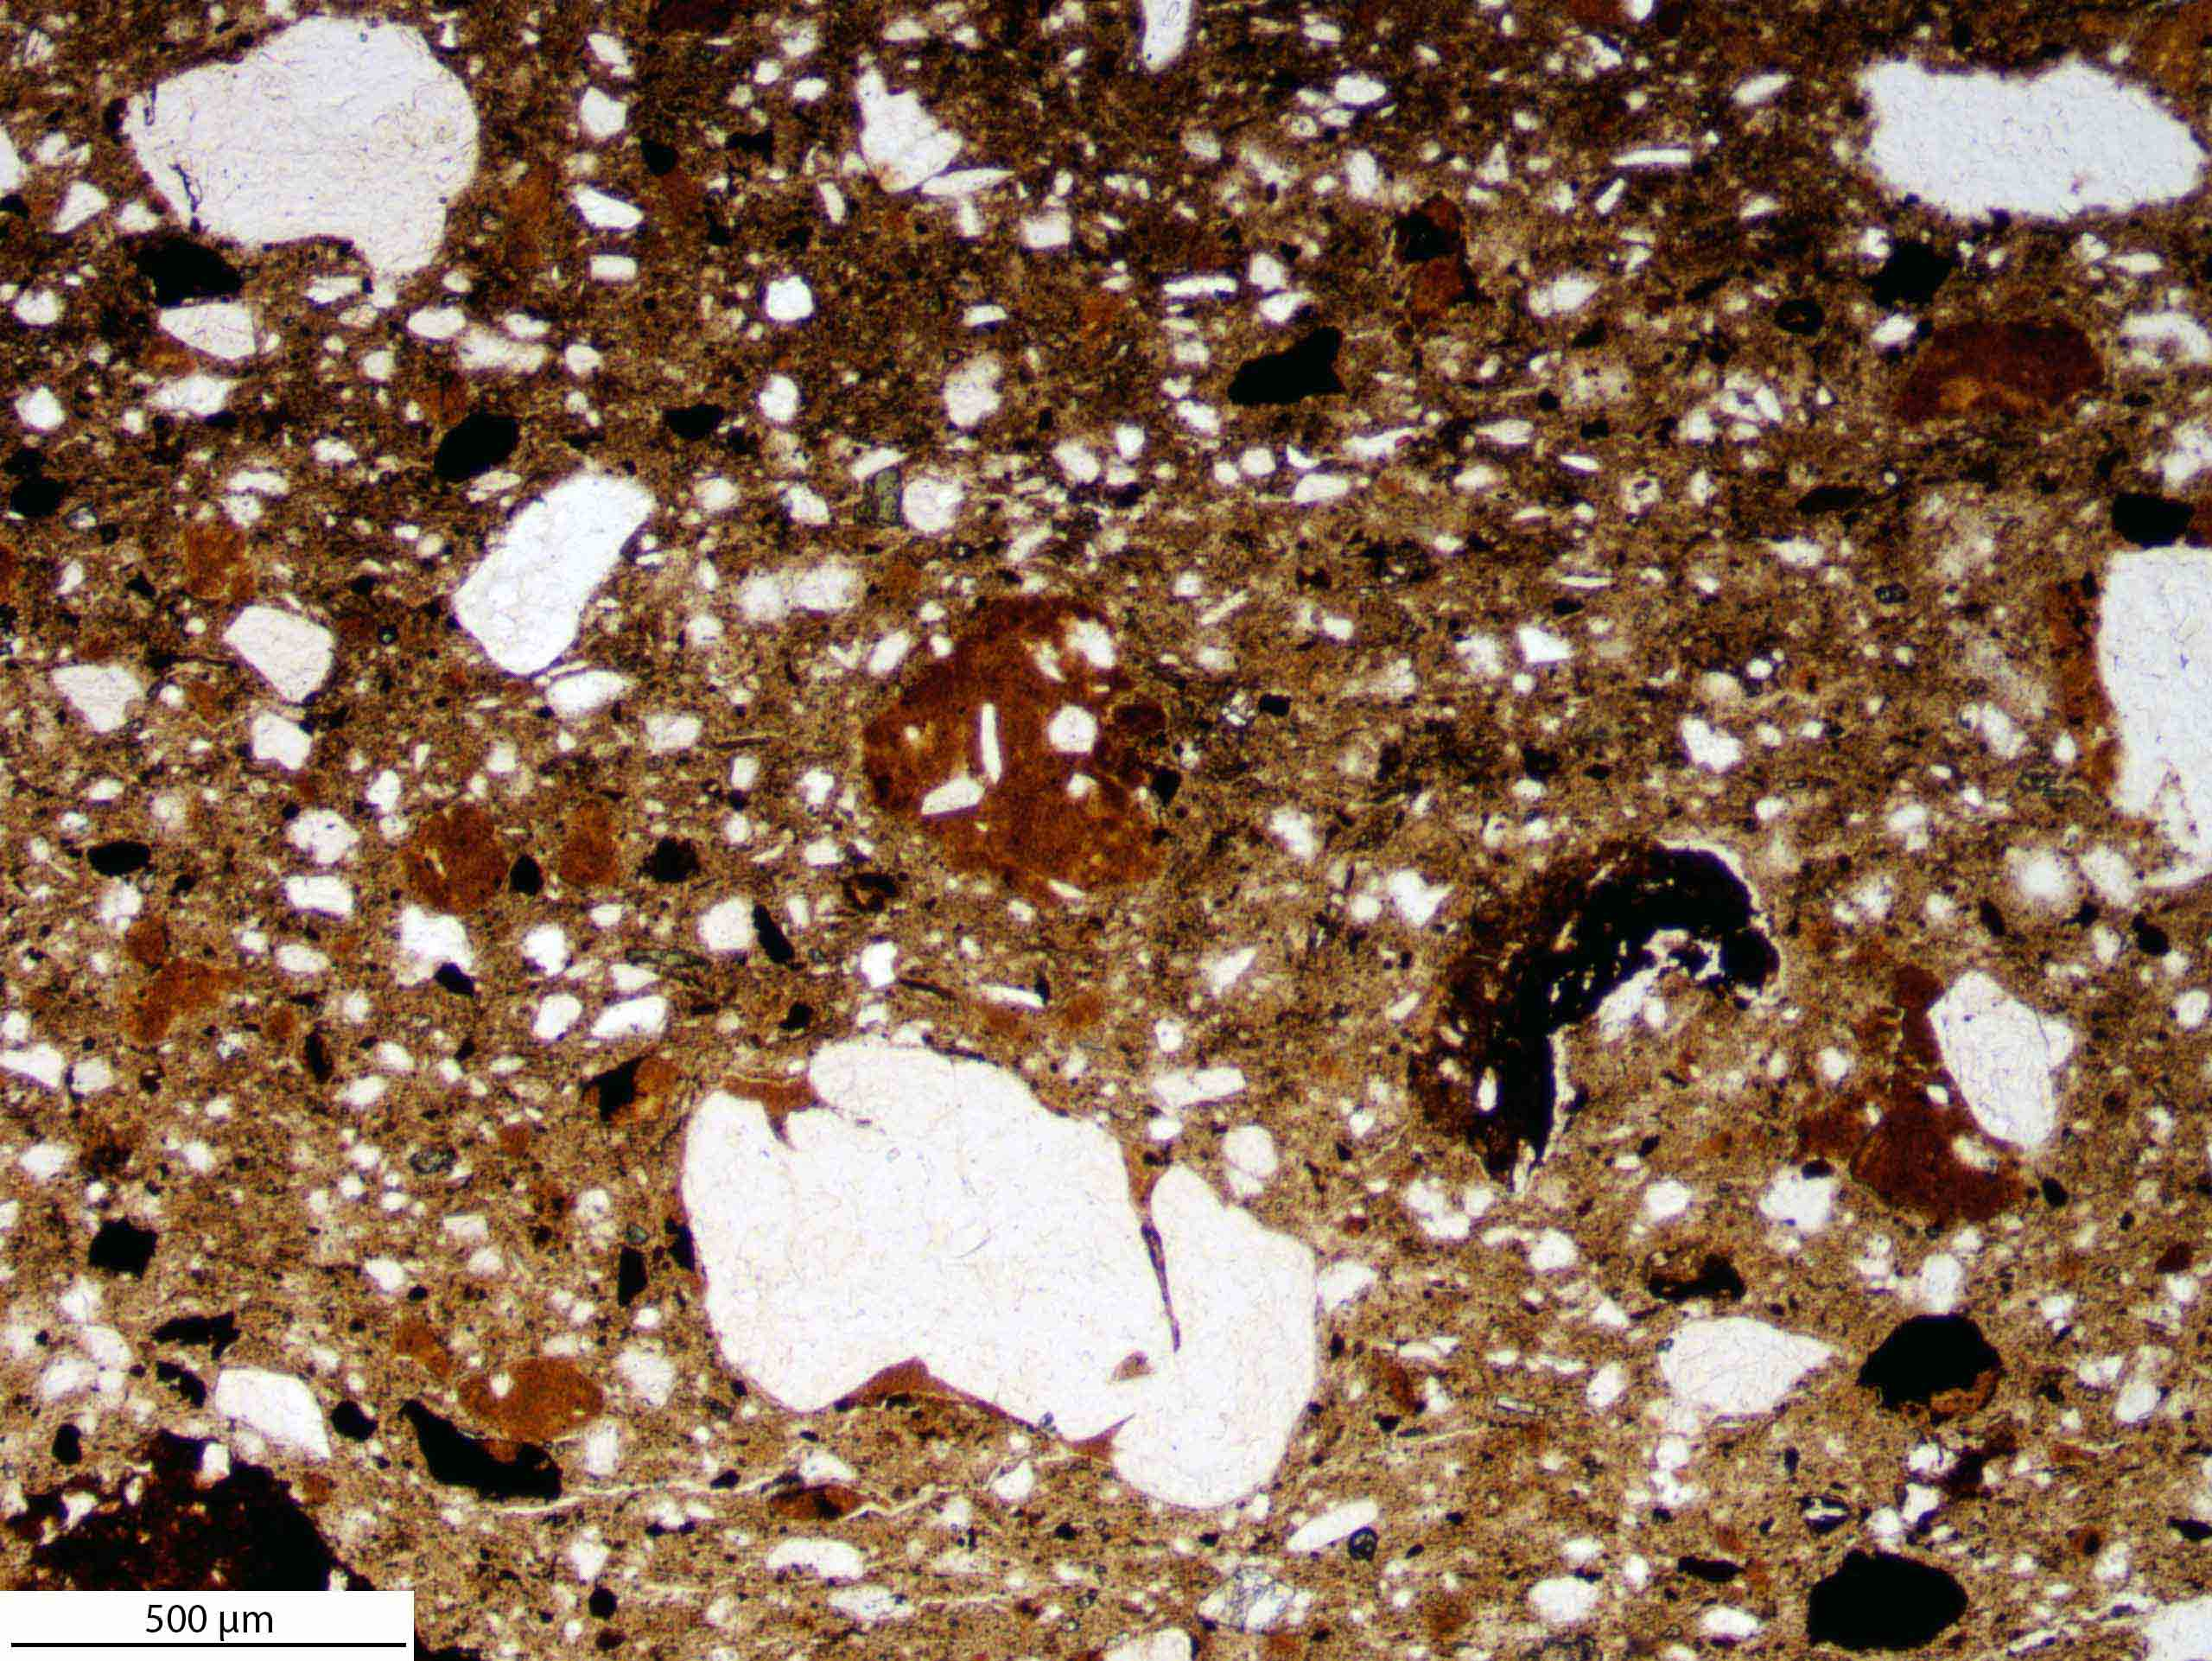
\includegraphics[width=\textwidth]{ThinSections/11-2_4x_PPL.jpg}
		\caption{[PPL]}
	\end{subfigure}\hspace{.5em}\hfill
	\begin{subfigure}[t]{.49\textwidth}
		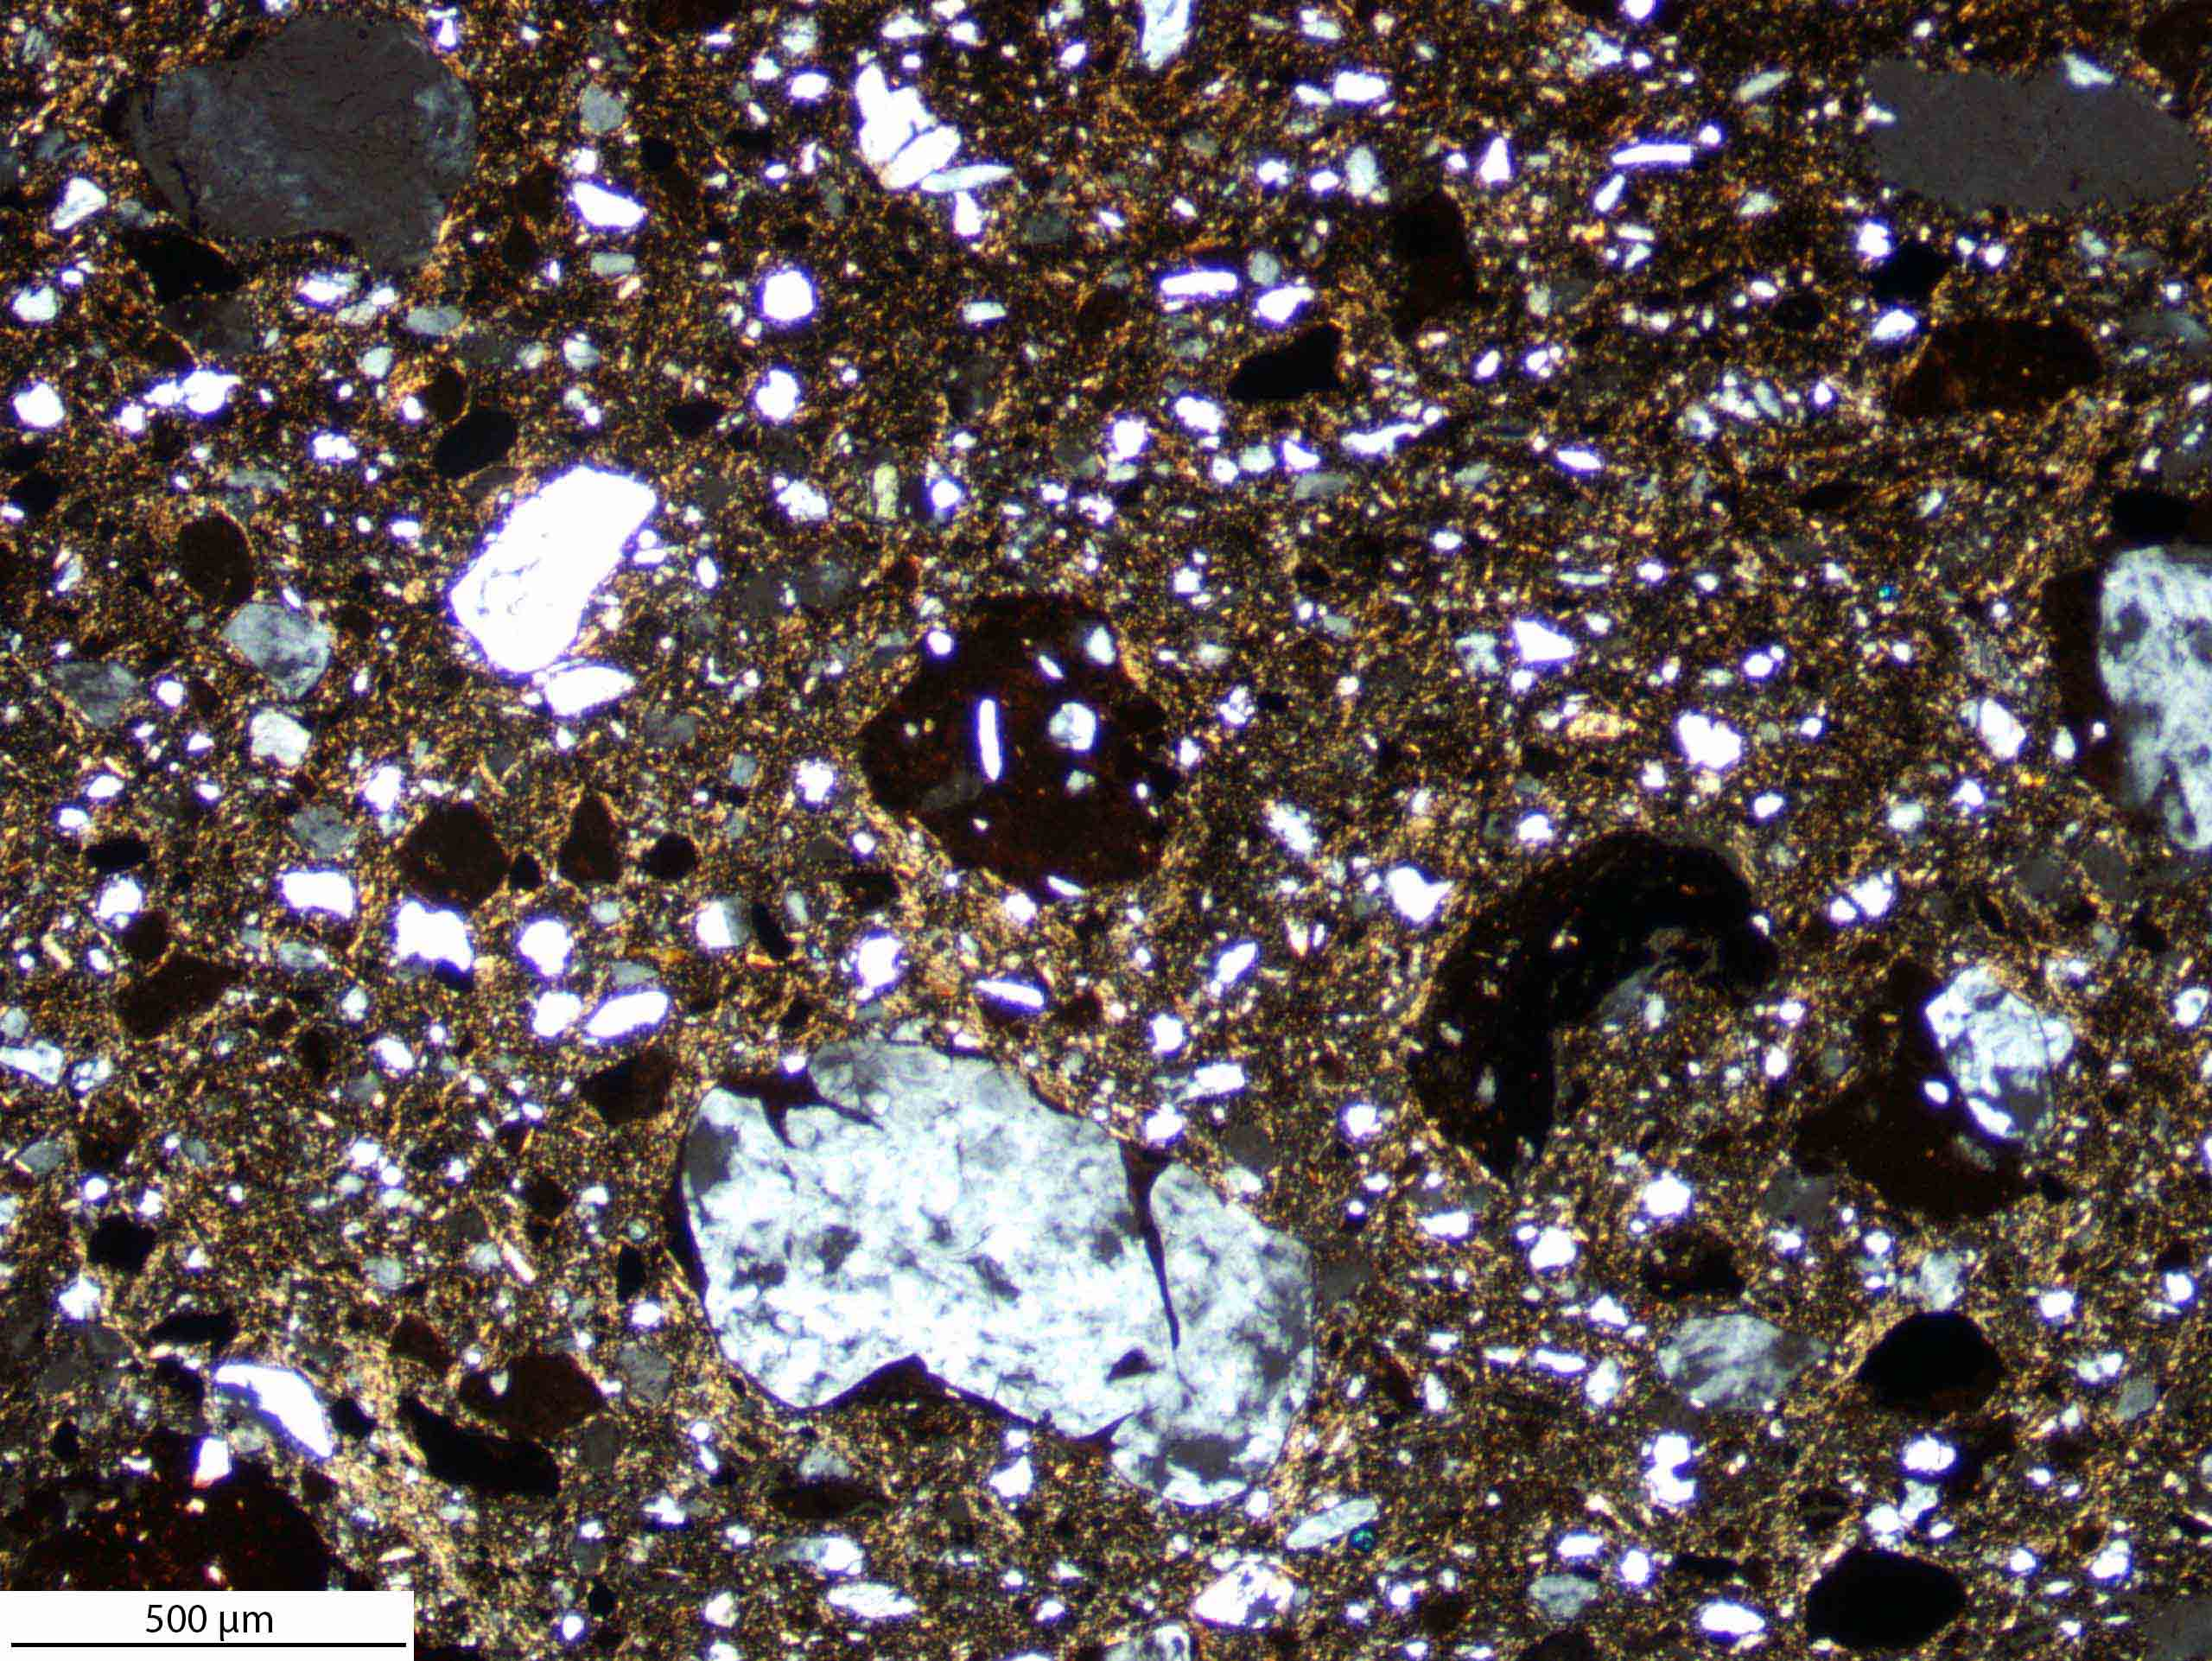
\includegraphics[width=\textwidth]{ThinSections/11-2_4x_XPL.jpg}
		\caption{[XPL]}
	\end{subfigure}
	\begin{subfigure}[t]{.49\textwidth}
		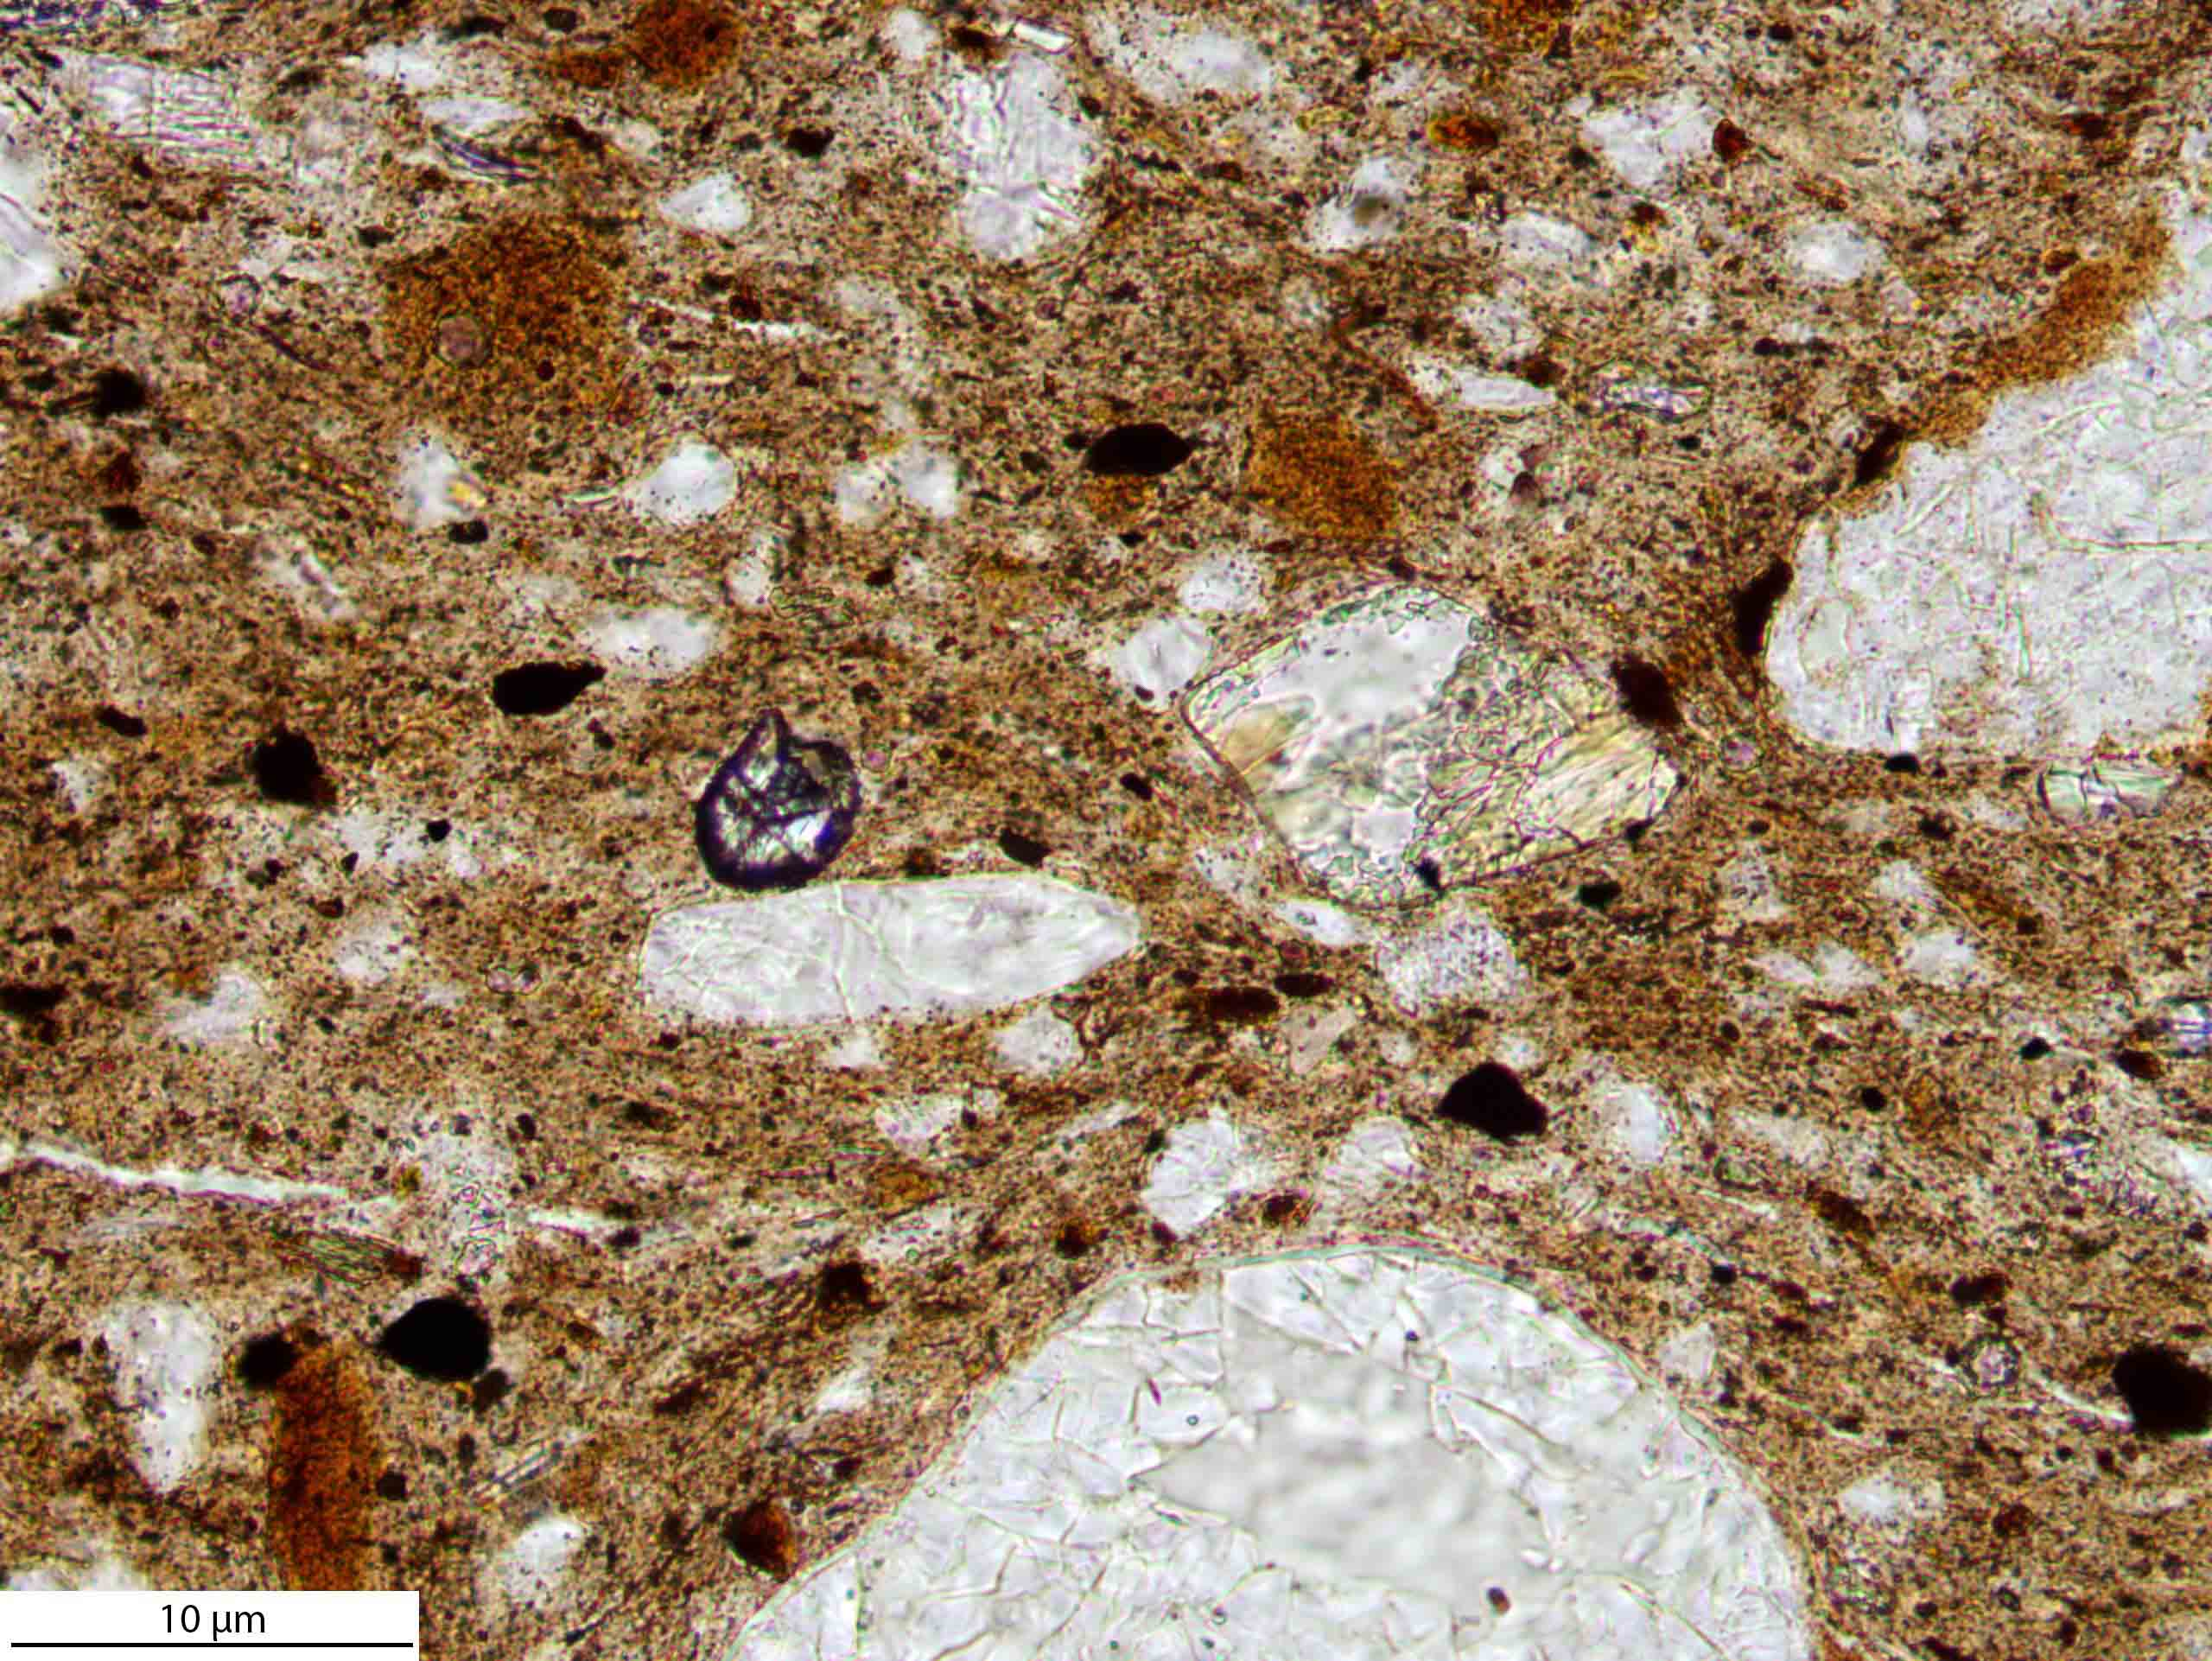
\includegraphics[width=\textwidth]{ThinSections/11-8_20x_PPL.jpg}
		\caption{Zircon \& staurolite [PPL]}
	\end{subfigure}\hspace{.5em}\hfill
	\begin{subfigure}[t]{.49\textwidth}
		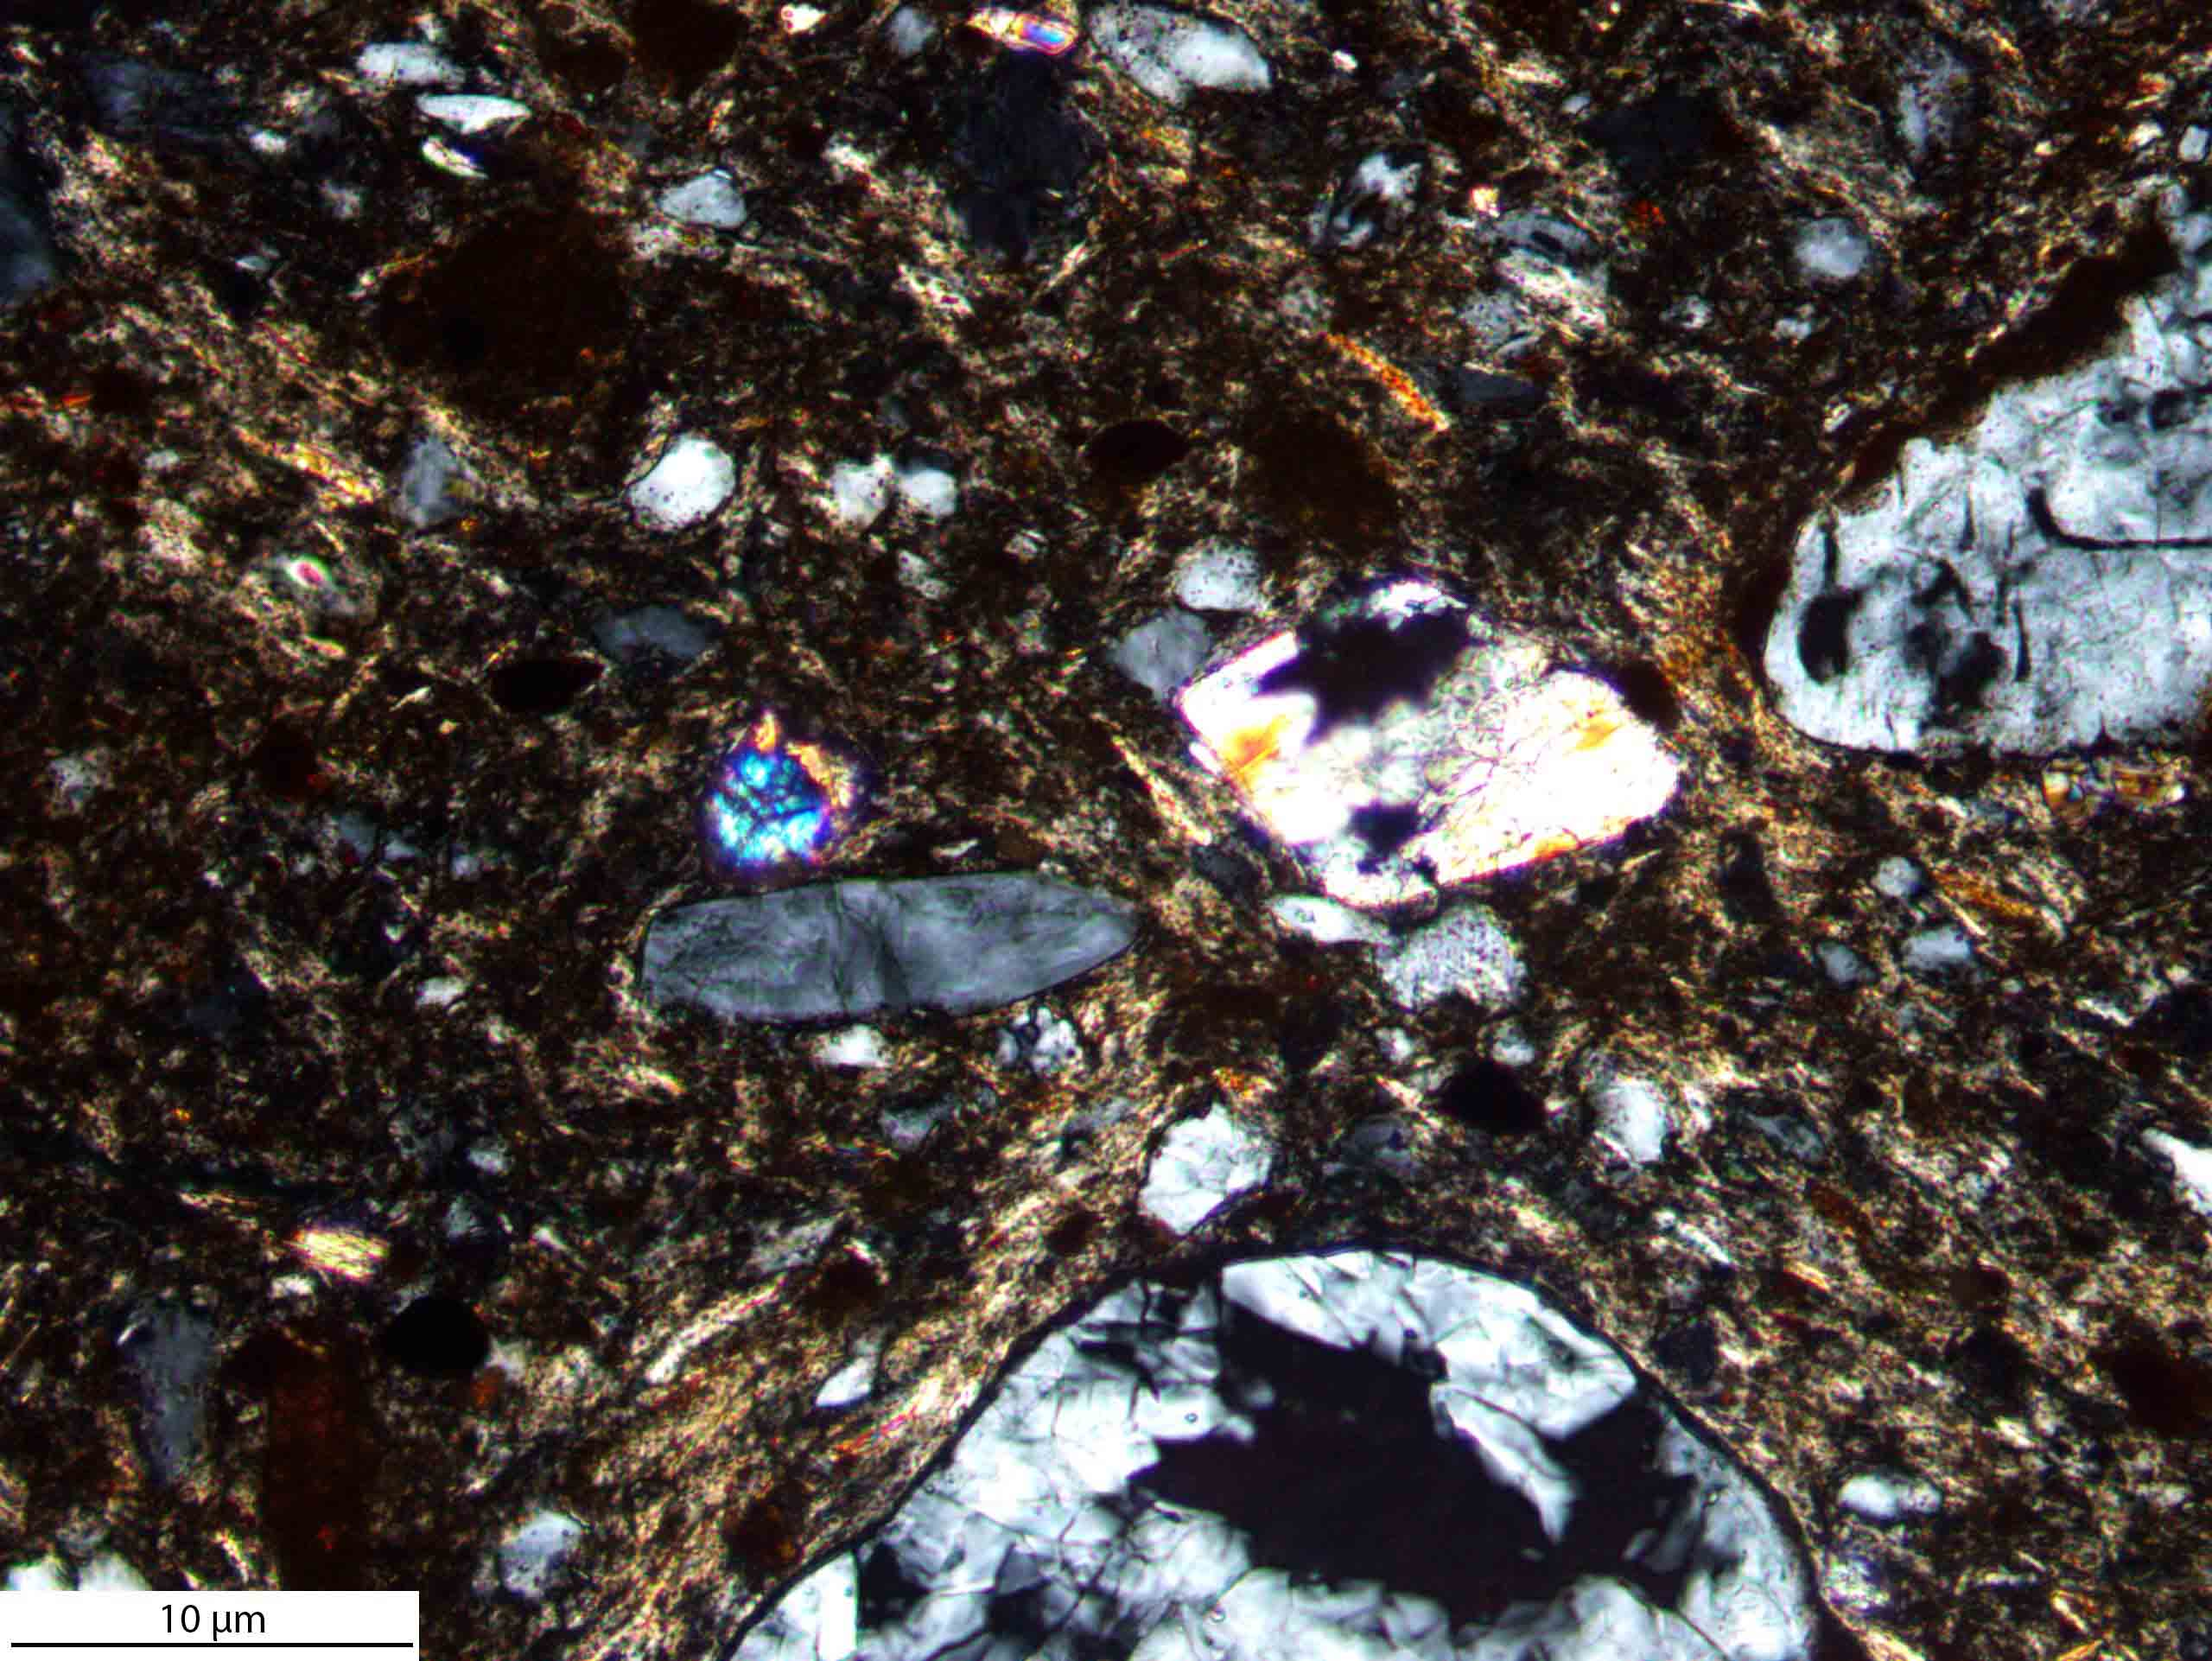
\includegraphics[width=\textwidth]{ThinSections/11-8_20x_XPL.jpg}
		\caption{Zircon \& staurolite [XPL]}
	\end{subfigure}
	\begin{subfigure}[t]{.32\textwidth}
		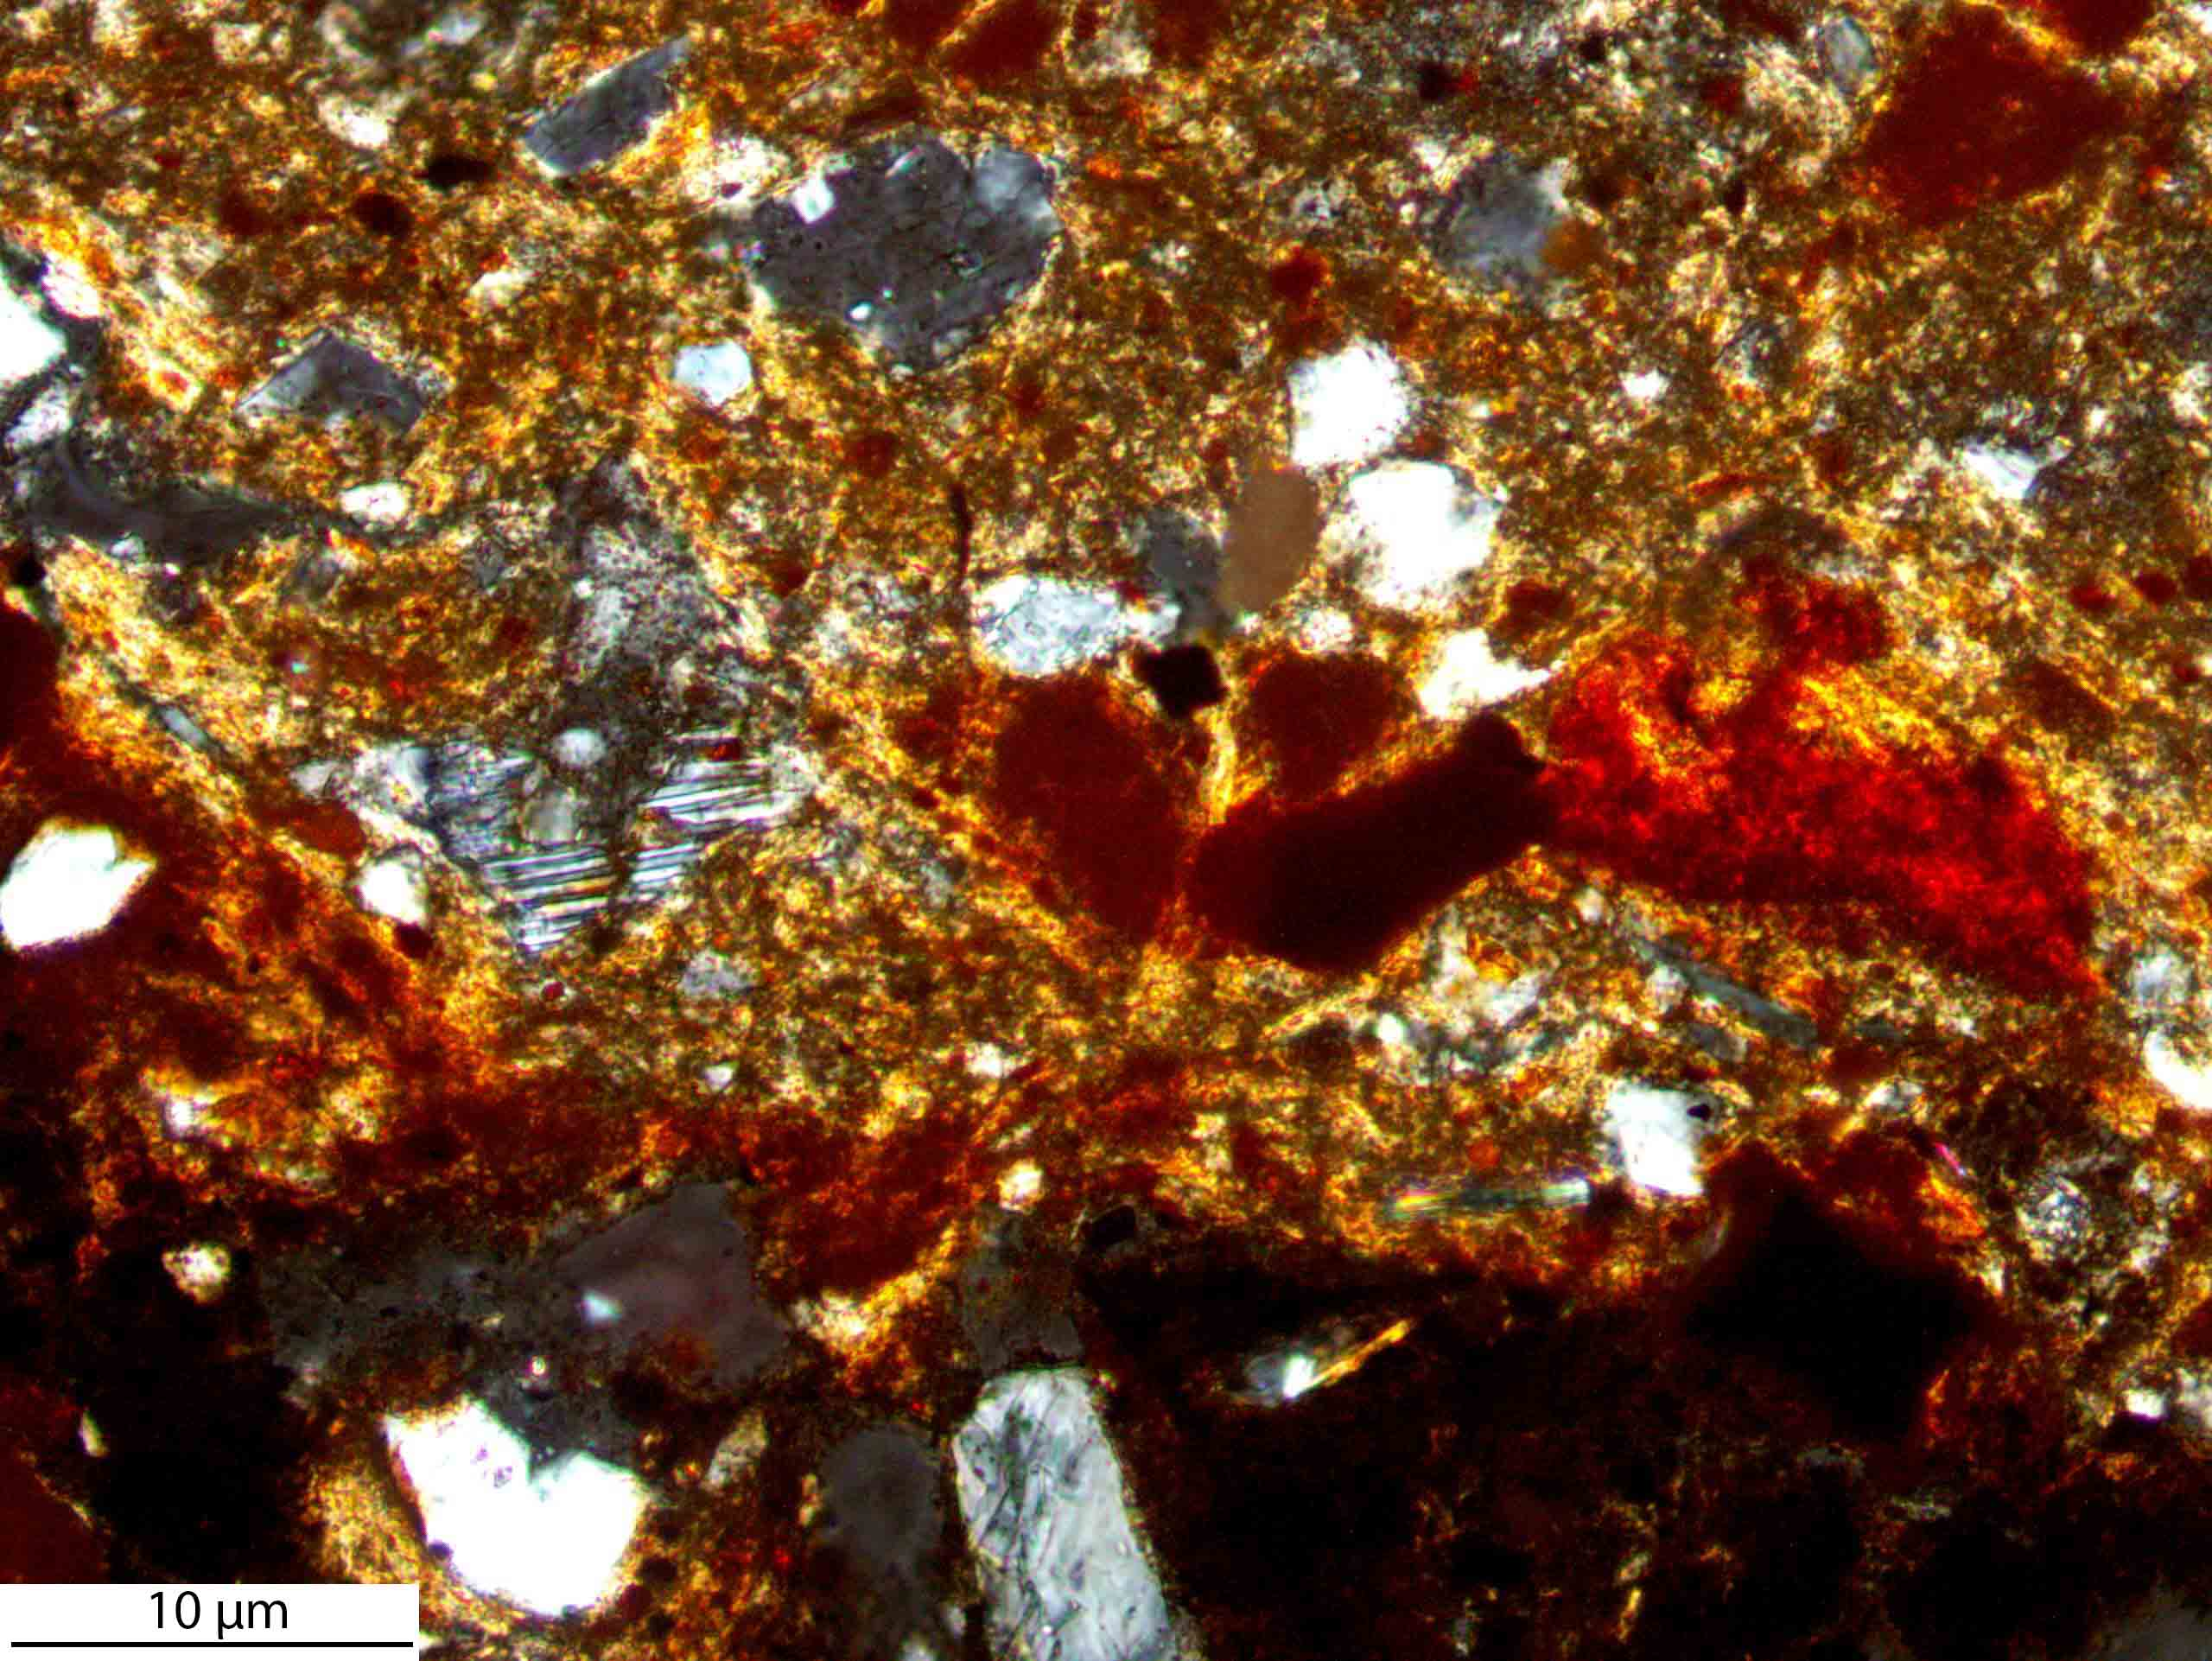
\includegraphics[width=\textwidth]{ThinSections/11-6_20x_XPL.jpg}
		\caption{Plagioclase [XPL]}
	\end{subfigure}\hspace{.1em}\hfill
	\begin{subfigure}[t]{.32\textwidth}
		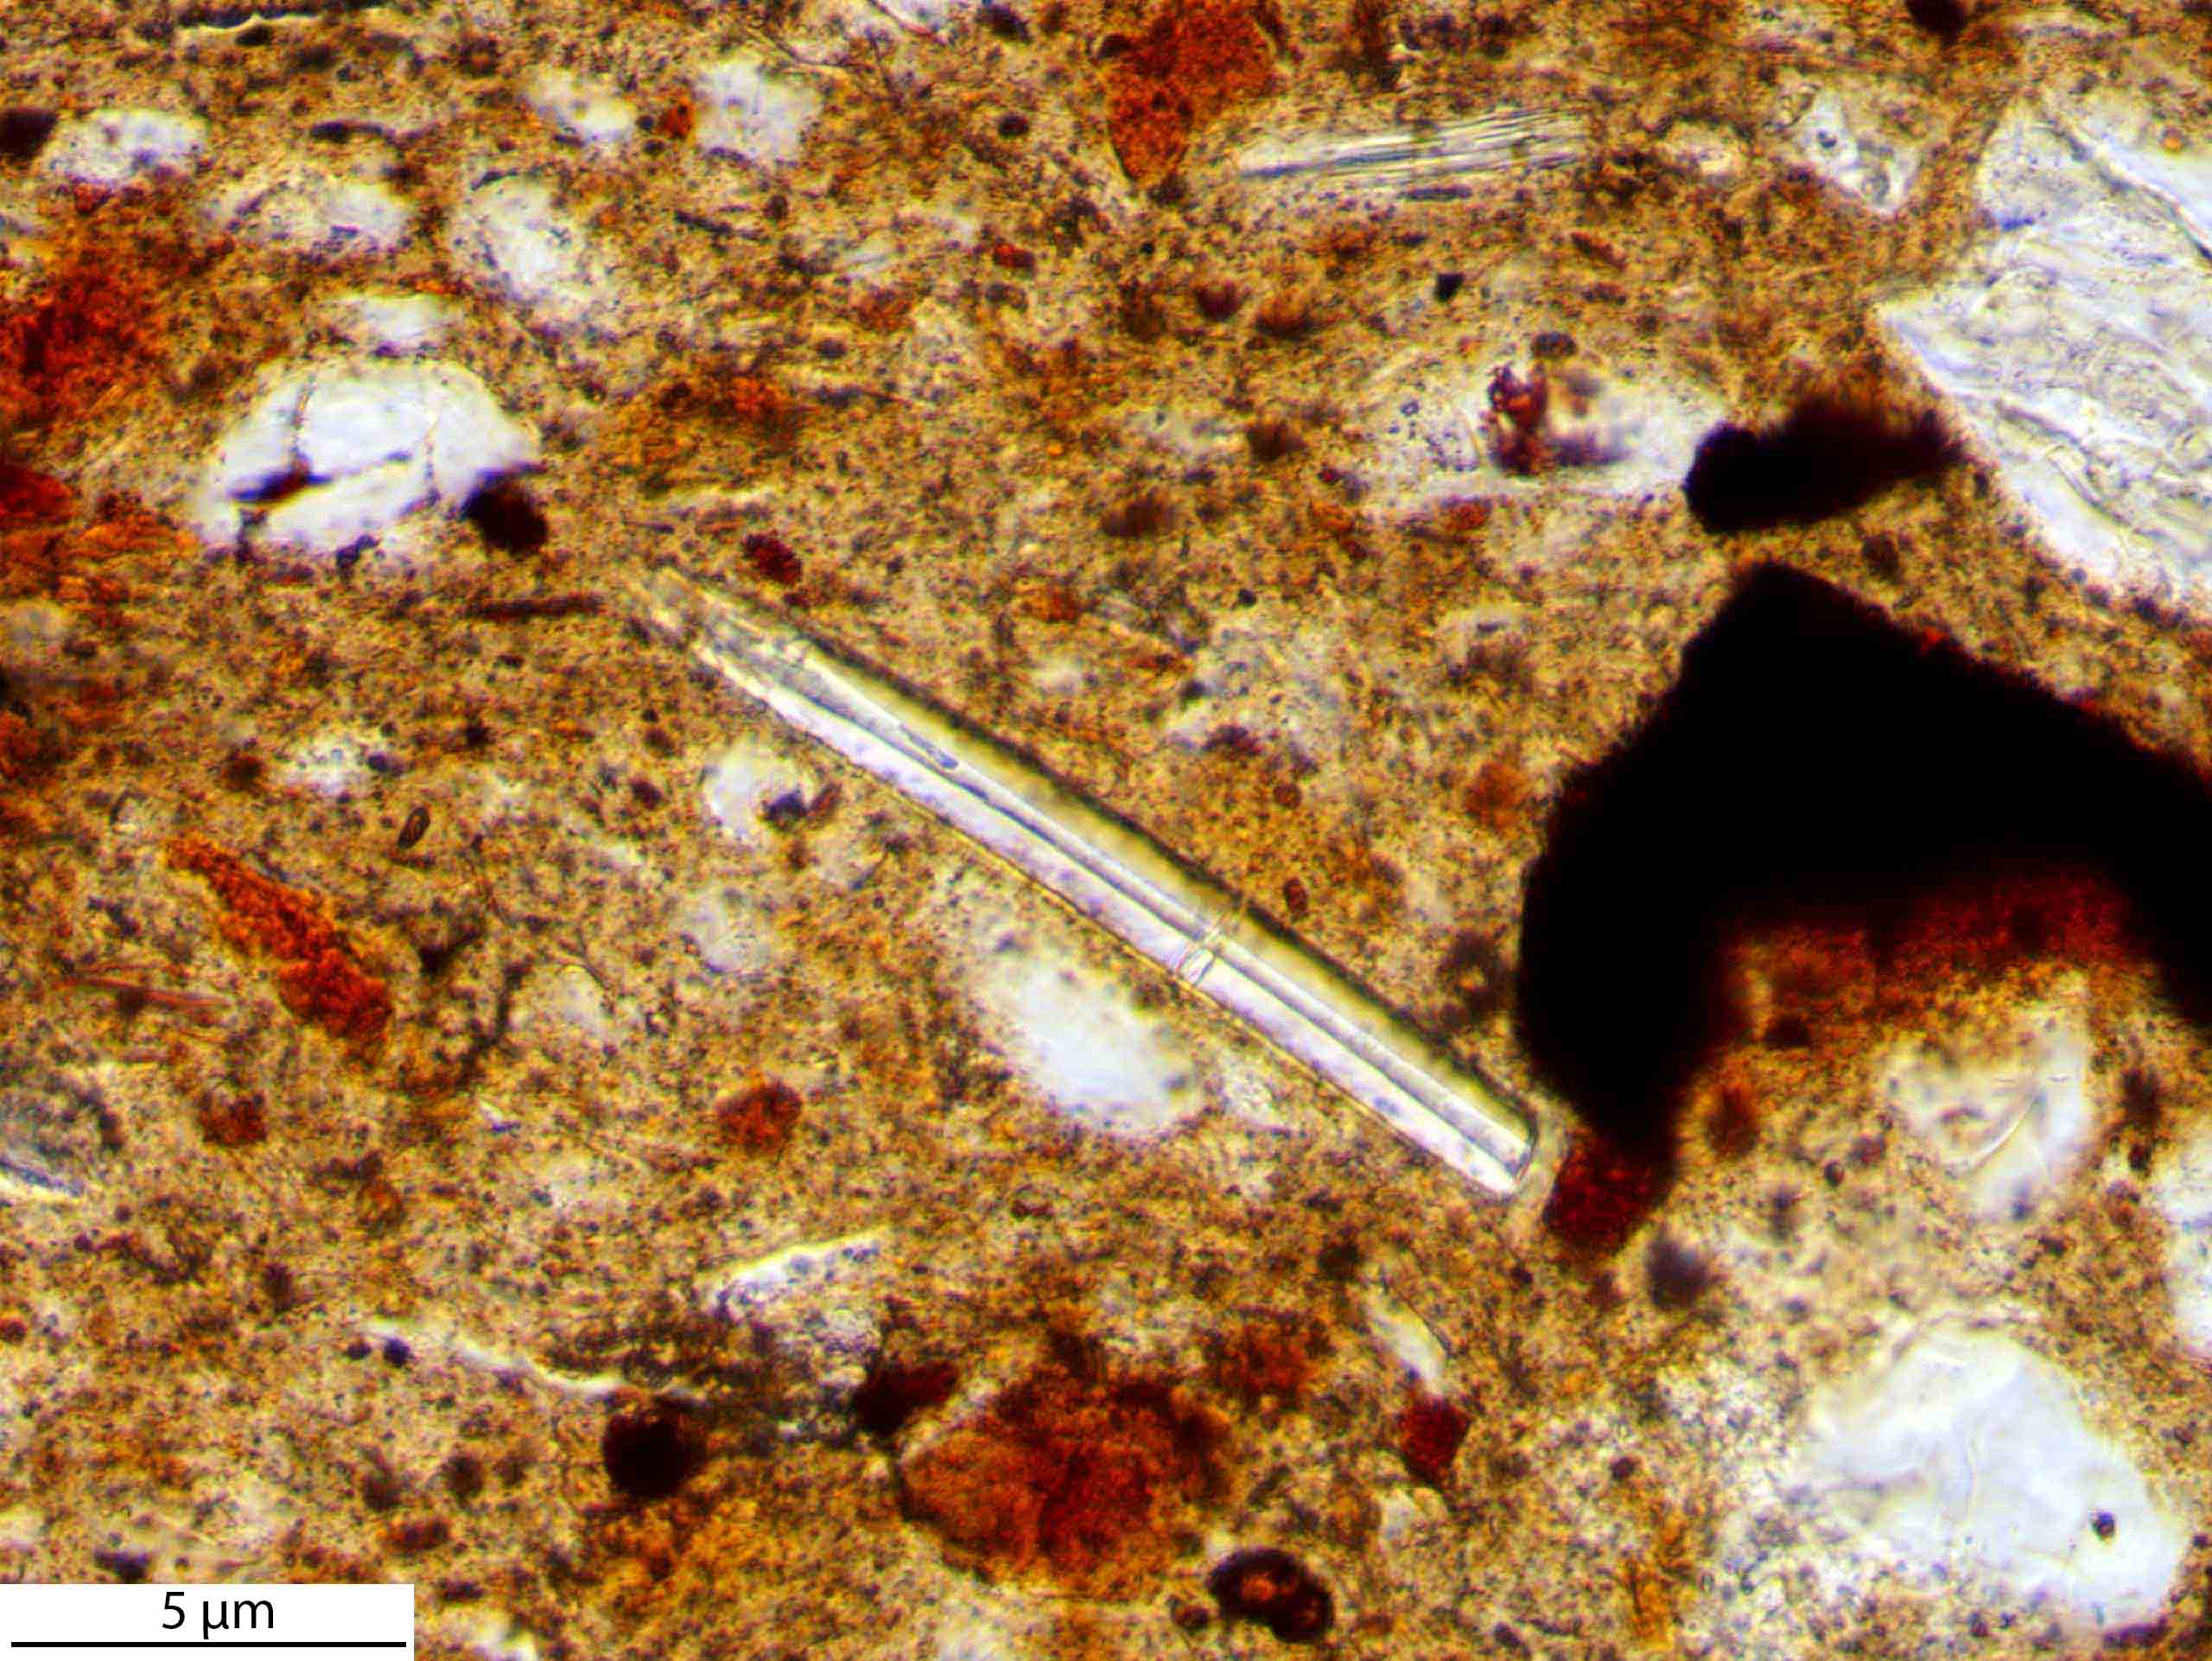
\includegraphics[width=\textwidth]{ThinSections/11-5_40x_PPL.jpg}
		\caption{Sponge spicule [PPL]}
	\end{subfigure}\hspace{.1em}\hfill
	\begin{subfigure}[t]{.32\textwidth}
		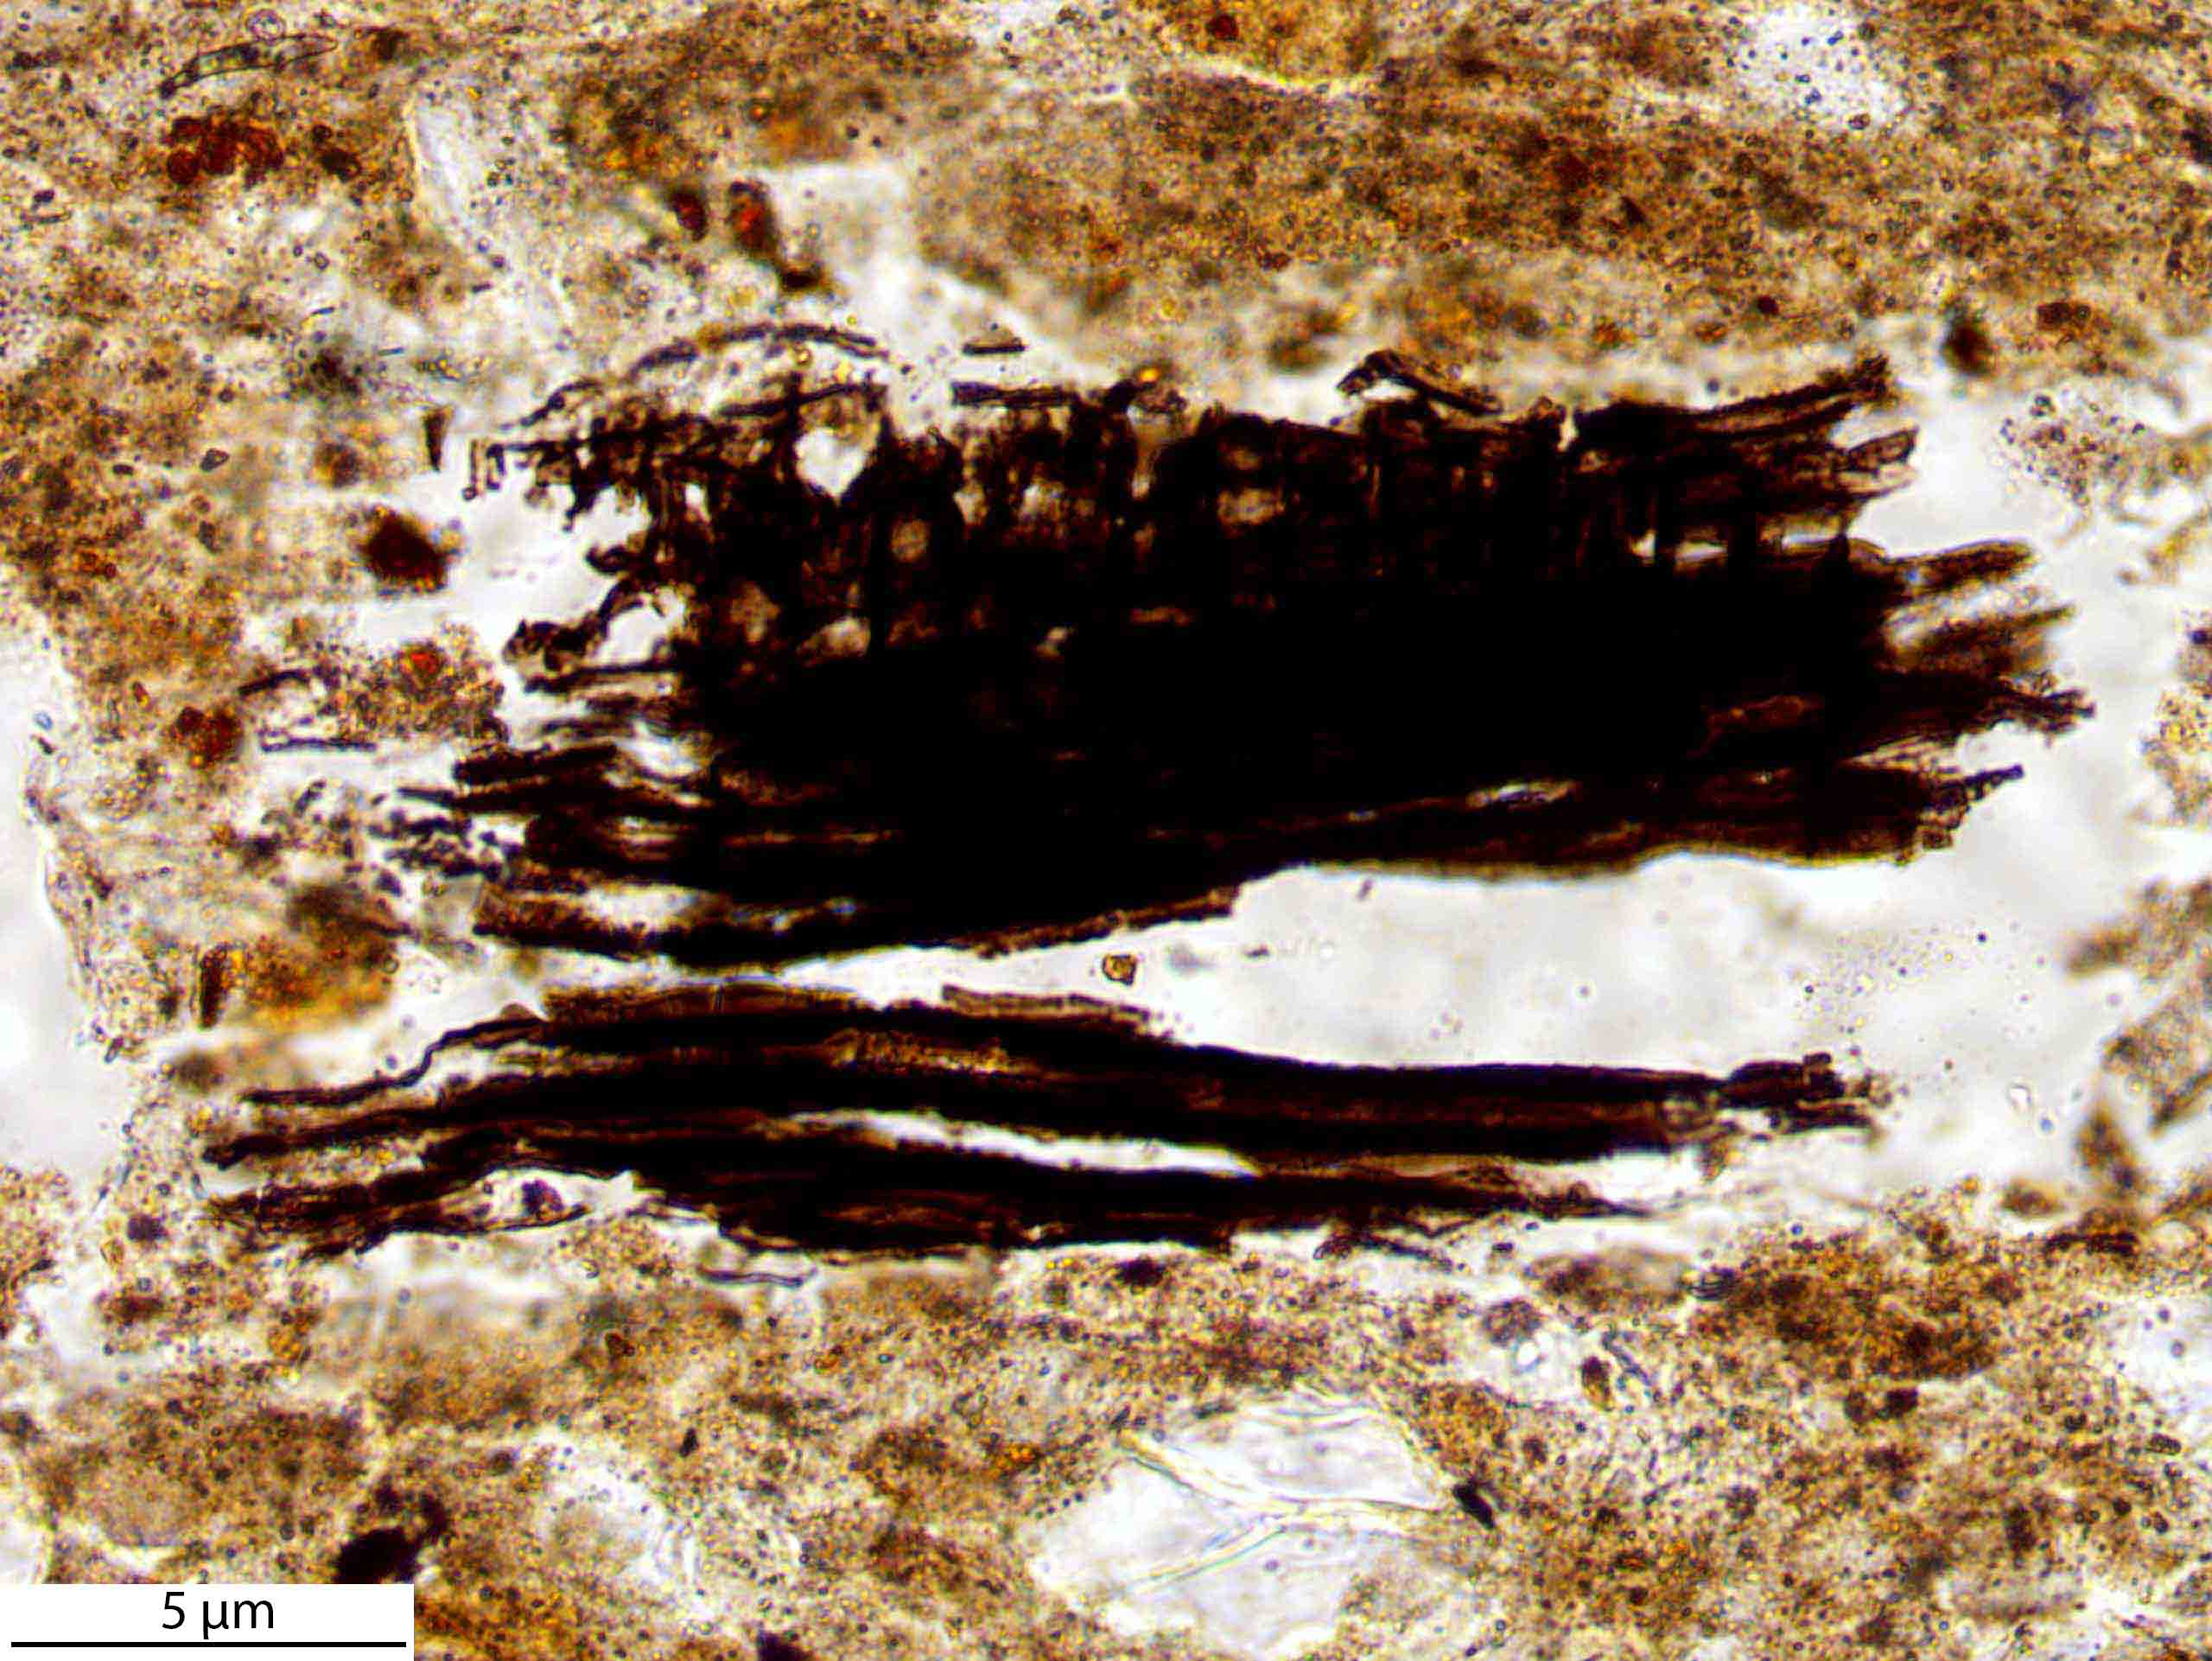
\includegraphics[width=\textwidth]{ThinSections/11-4_40x_PPL.jpg}
		\caption{Plant matter [PPL]}
	\end{subfigure}
	\caption{}
	\label{fig:11_pik}
\end{figure}

\newpage\subsection{PIK 87/1-2:70 (pik\#55; Ebambe style; Fig.~\ref{fig:thinsections}A--C)}

\begin{multicols}{2}
\noindent The fine fraction is homogeneous and non-calcareous (light yellowish [PPL]) with unistriated b-fabric. The section shows nearly no or very narrow voids. The dominant component of the coarse fraction are sponge spicules, mostly cut longitudinal and oriented wall-parallel in relation to the plane of the section, and a very fine (sub-)angular quartz fraction. Rare are sub-angular homogeneous clay pellets, muscovite, tourmaline, and zircon. The c/f-related distribution pattern is single-spaced porphyric (open porphyric if only quartz grains are regarded as coarse material).
\end{multicols}

% sponge spicules > category as shell in Stoops

%\vfill
\begin{figure}[H]
	\centering
	\begin{subfigure}[t]{.49\textwidth}
		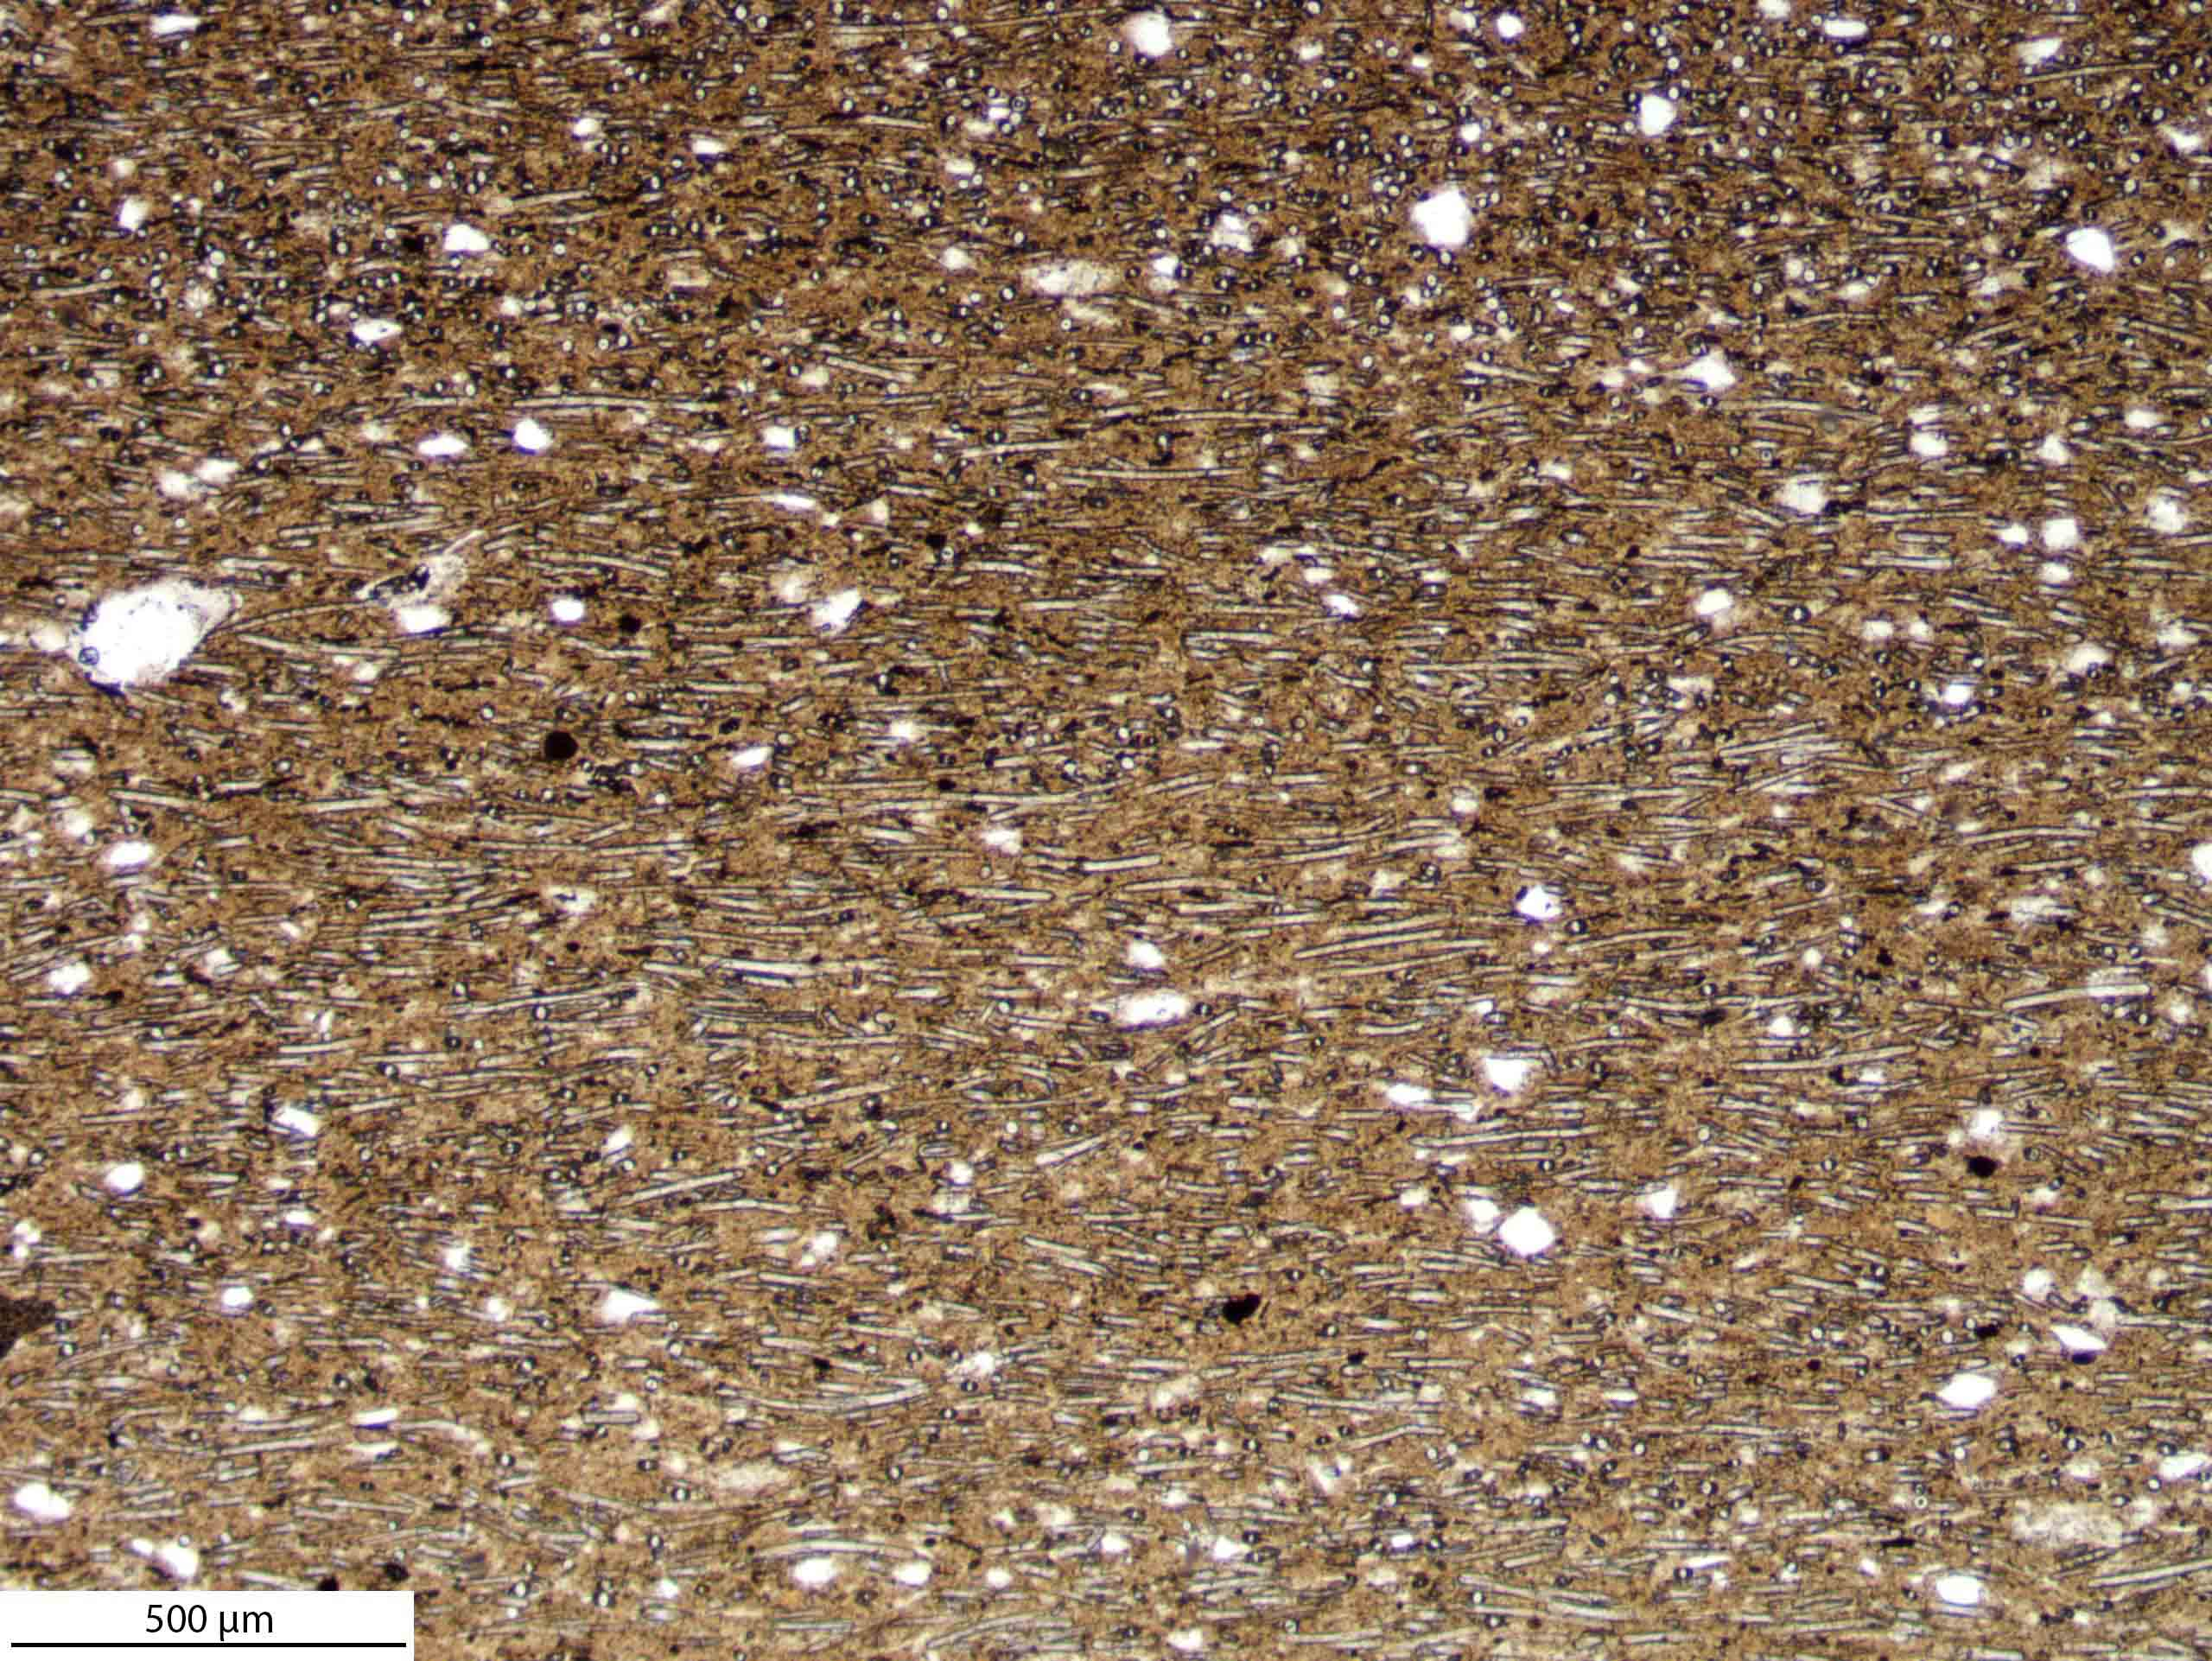
\includegraphics[width=\textwidth]{ThinSections/55-4_4x_PPL.jpg}
		\caption{[PPL]}
	\end{subfigure}\hspace{.5em}\hfill
	\begin{subfigure}[t]{.49\textwidth}
		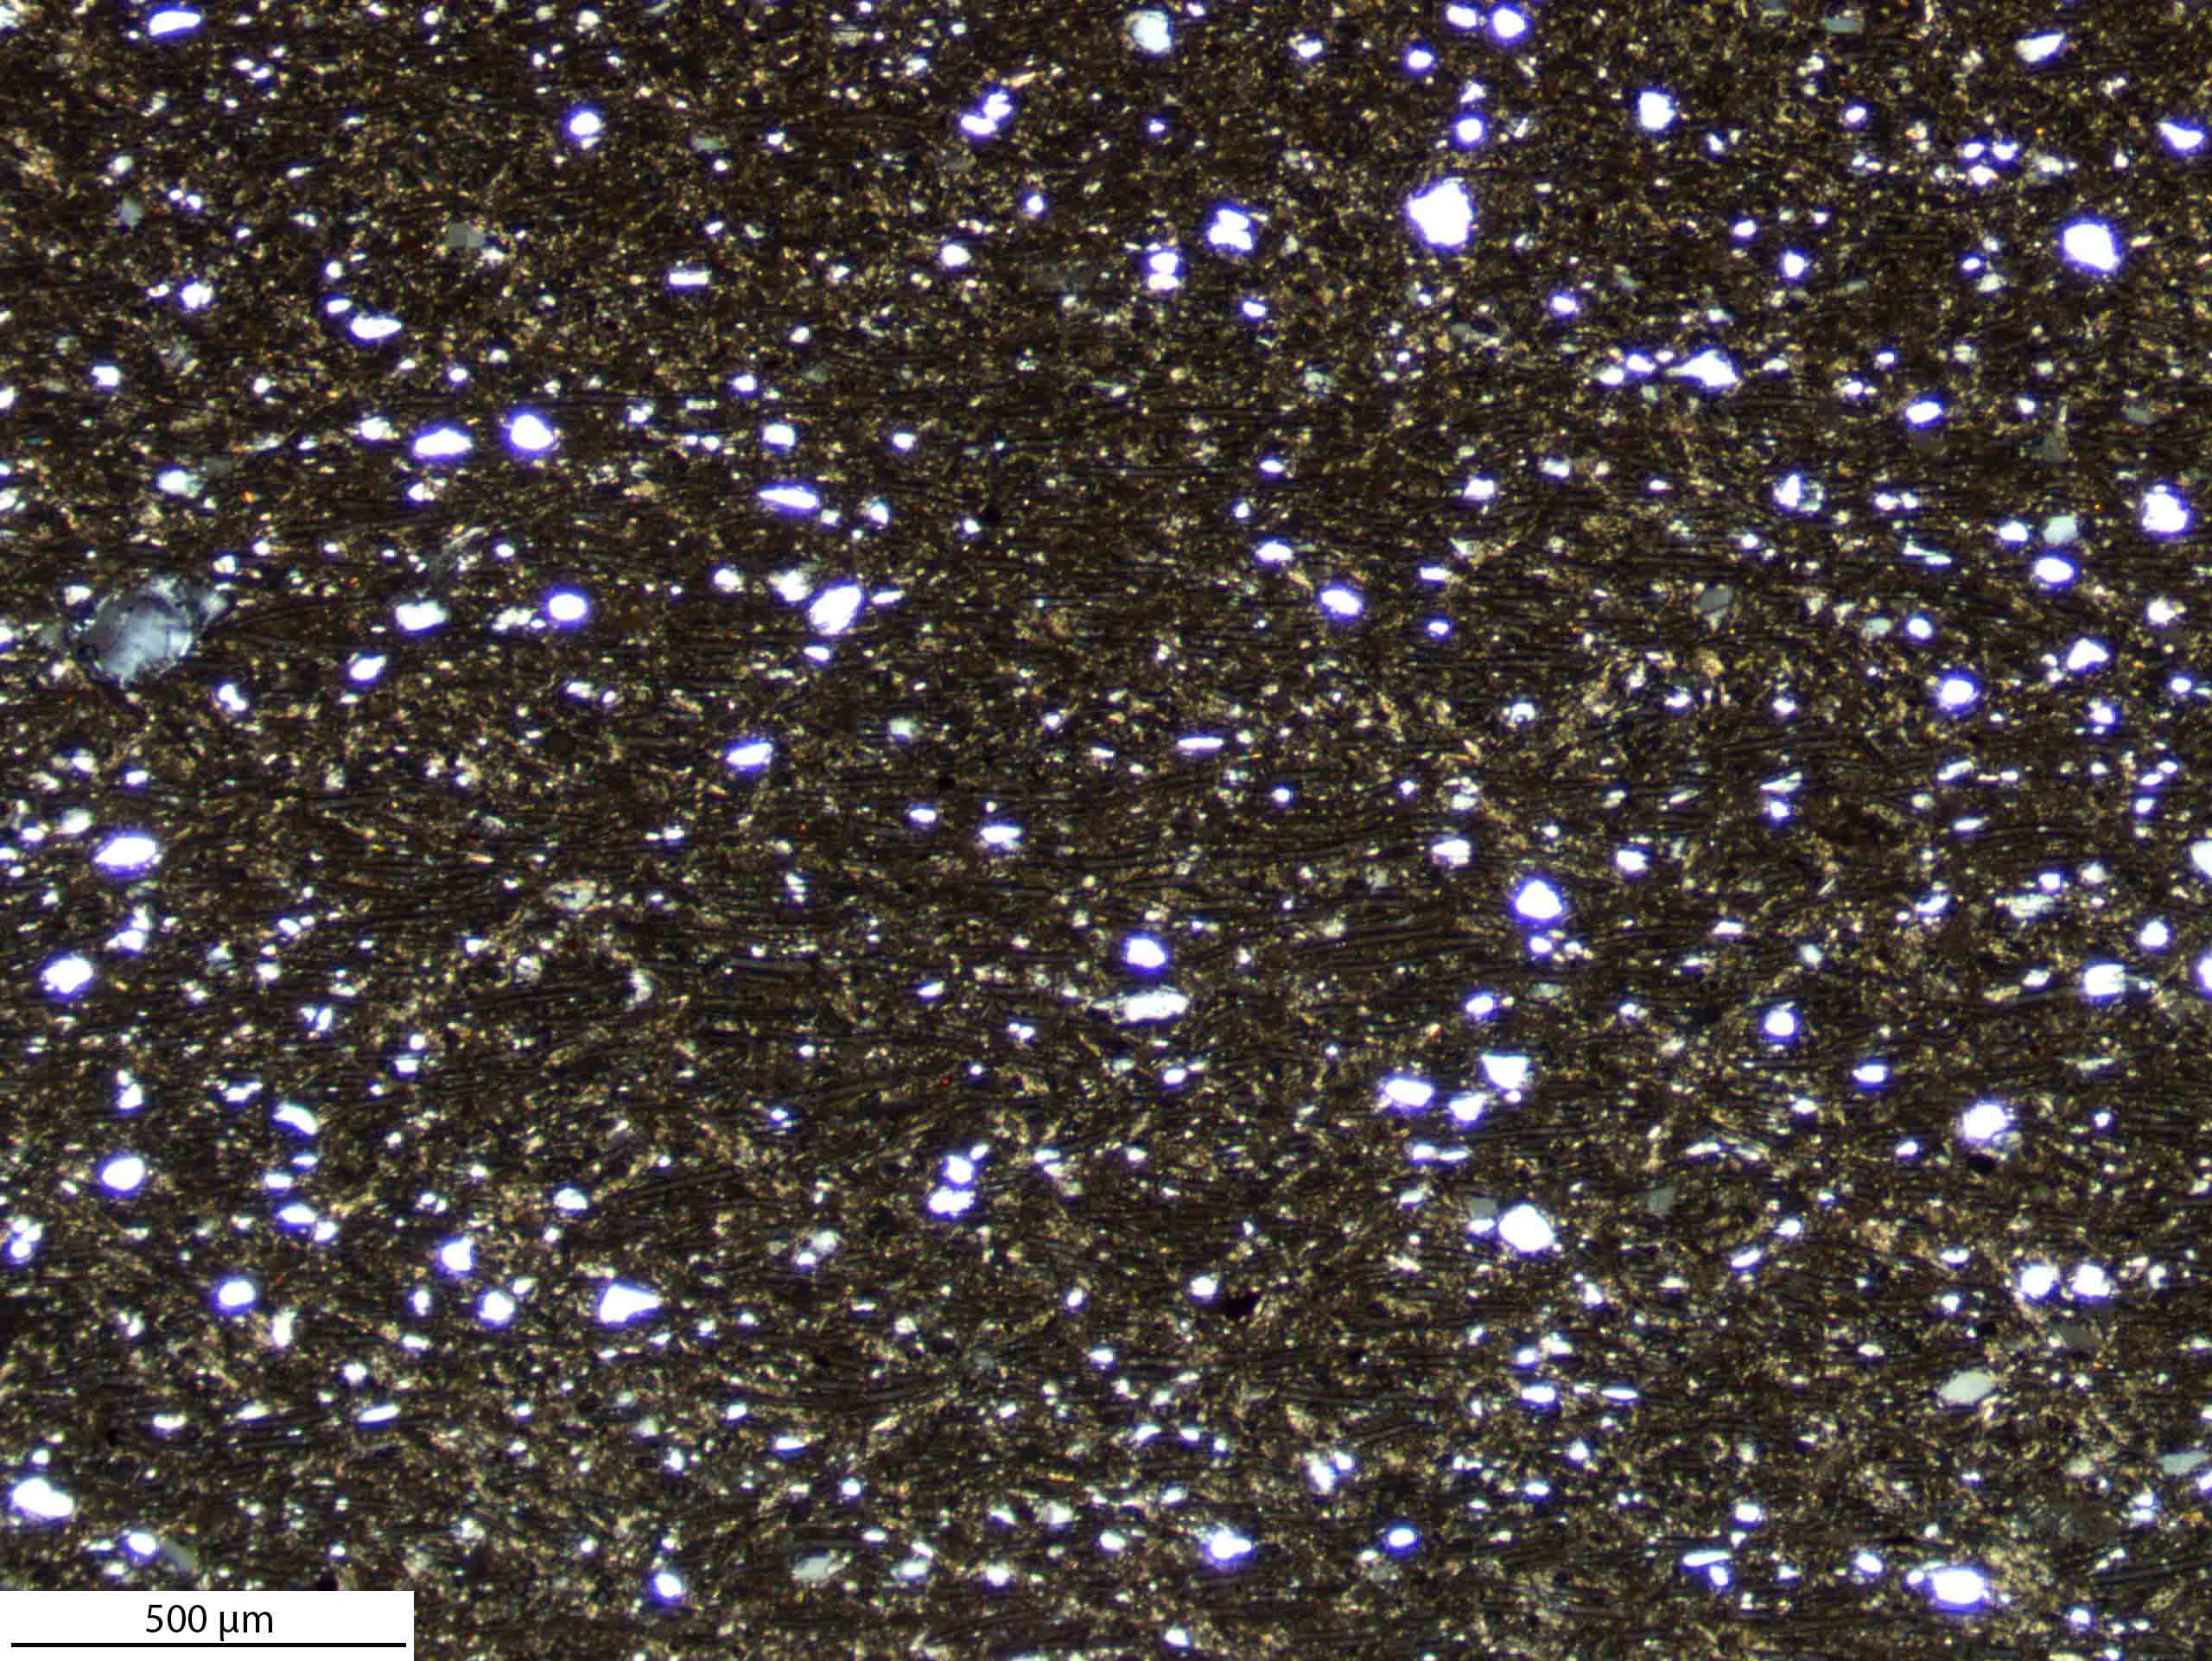
\includegraphics[width=\textwidth]{ThinSections/55-4_4x_XPL.jpg}
		\caption{[XPL]}
	\end{subfigure}
	\begin{subfigure}[t]{.49\textwidth}
		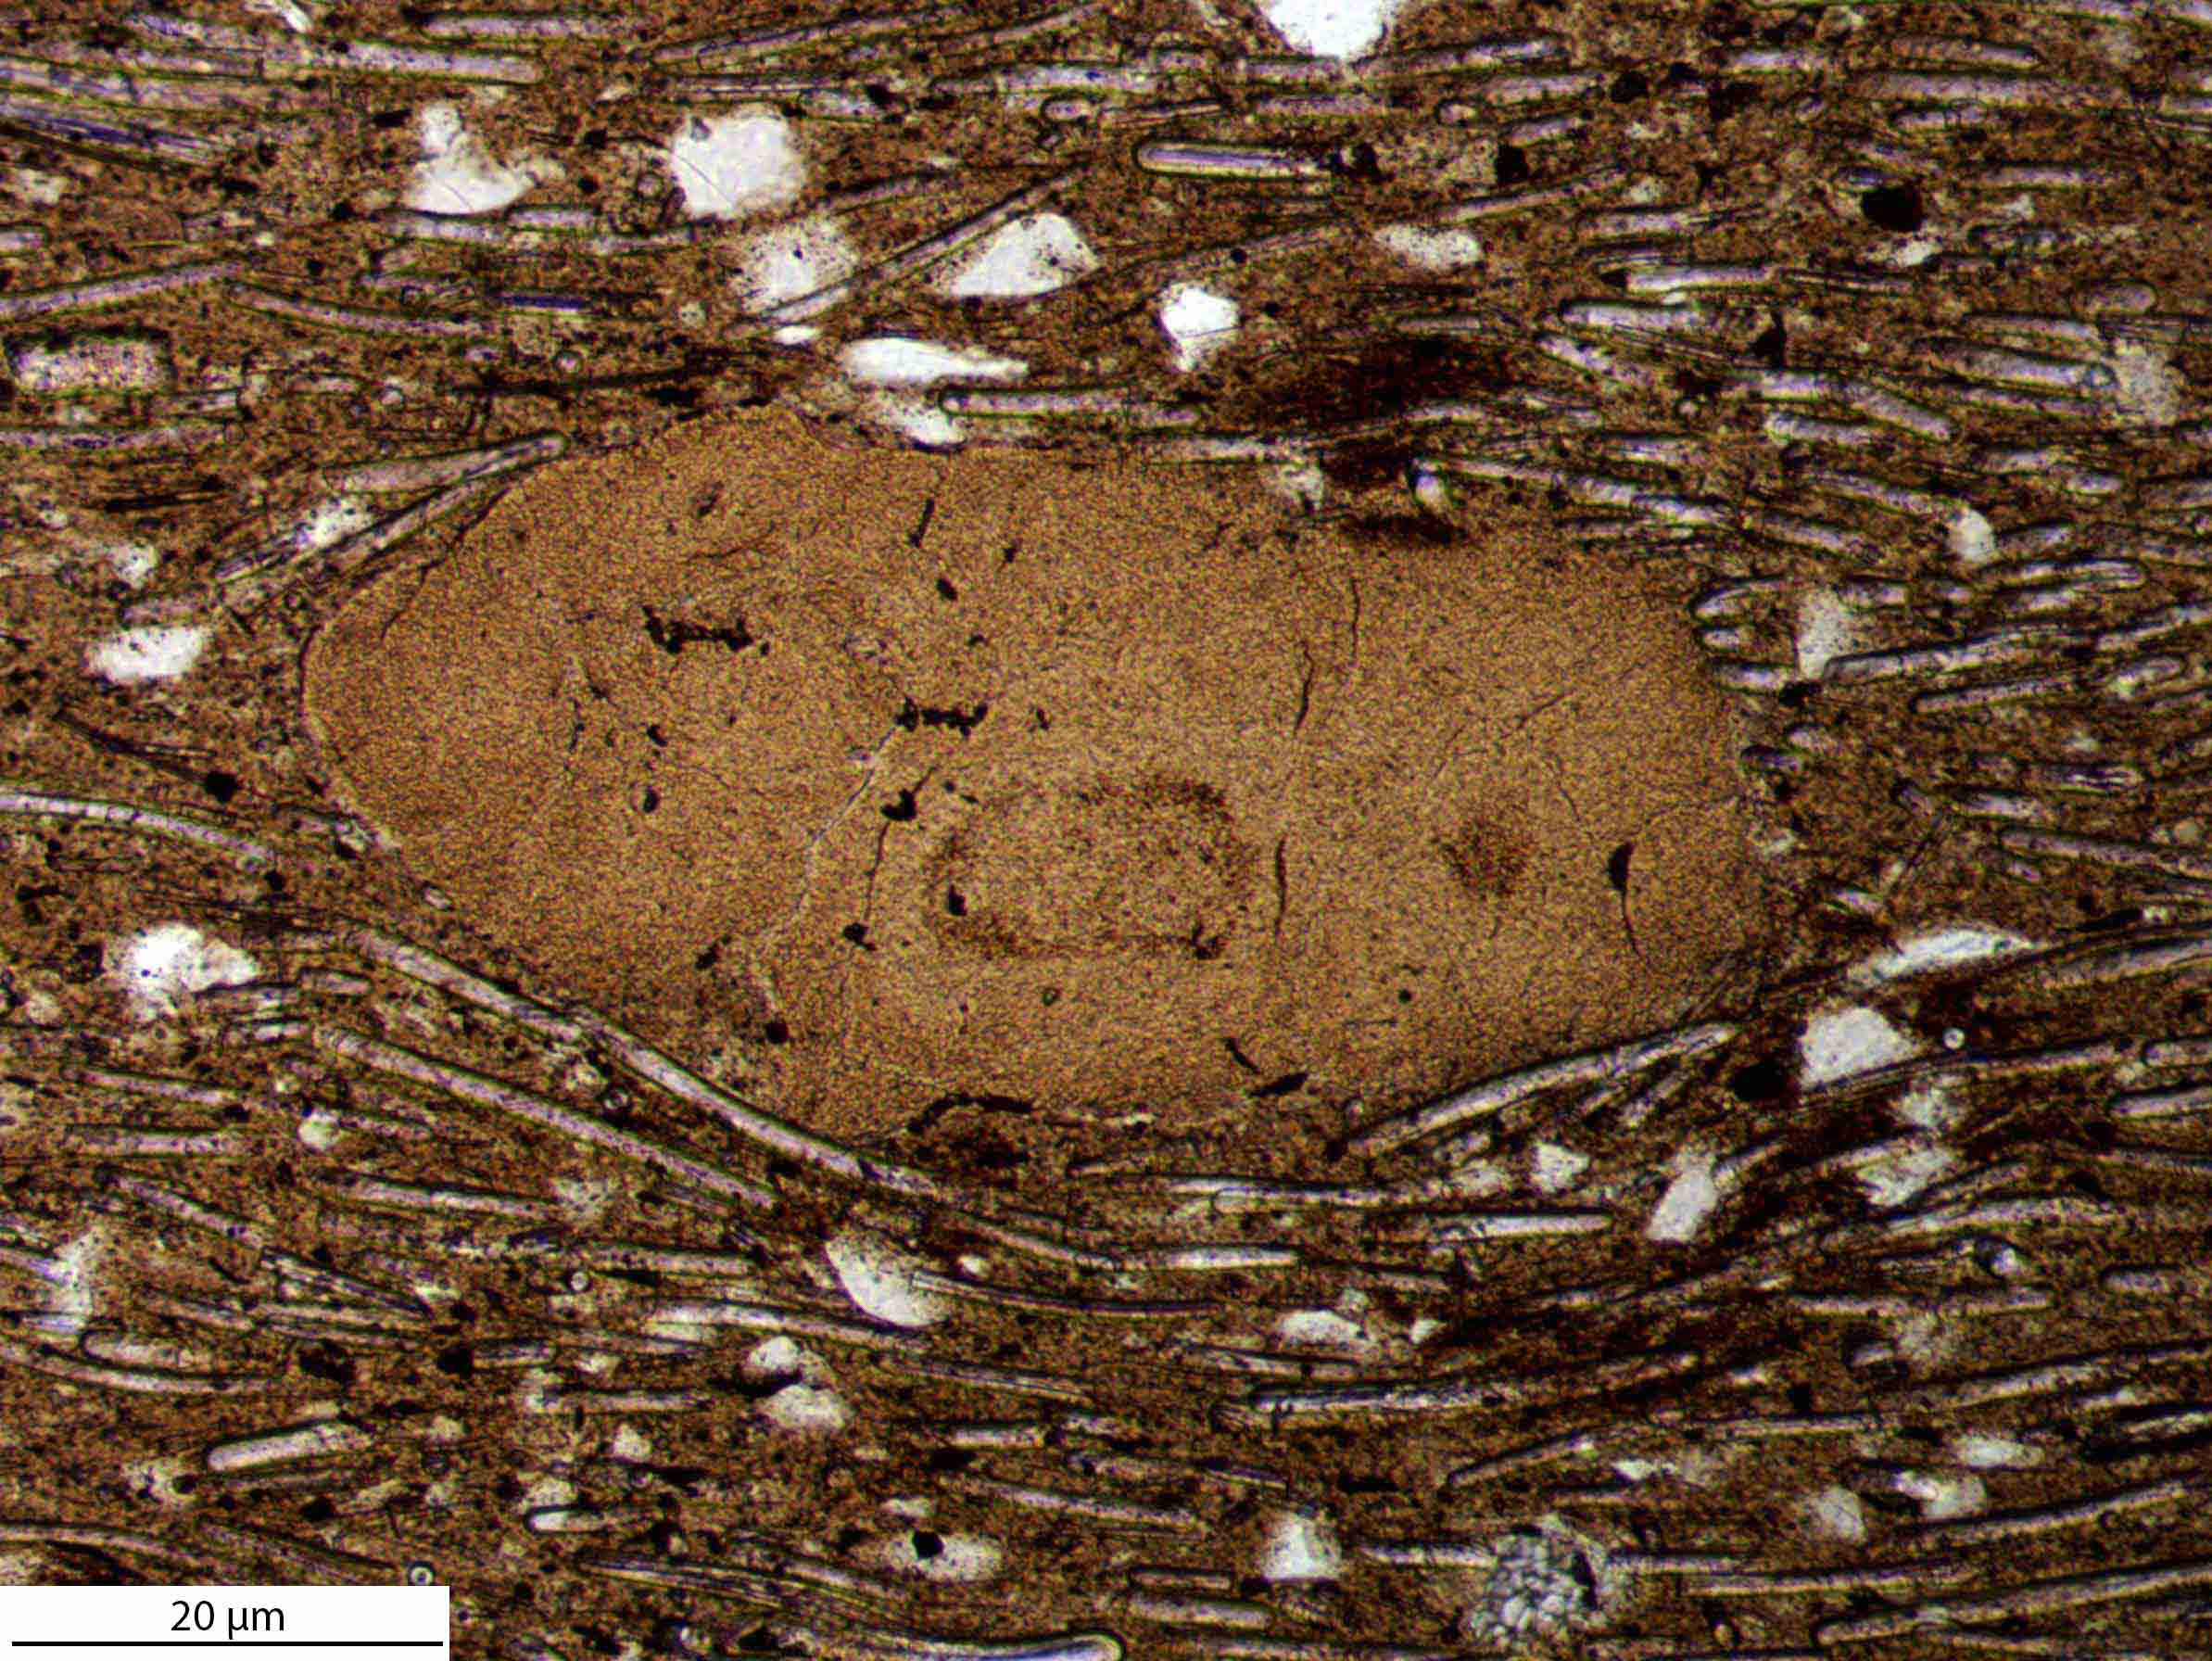
\includegraphics[width=\textwidth]{ThinSections/55_10x_PPL.jpg}
		\caption{Clay pellet [PPL]}
	\end{subfigure}\hspace{.5em}\hfill
	\begin{subfigure}[t]{.49\textwidth}
		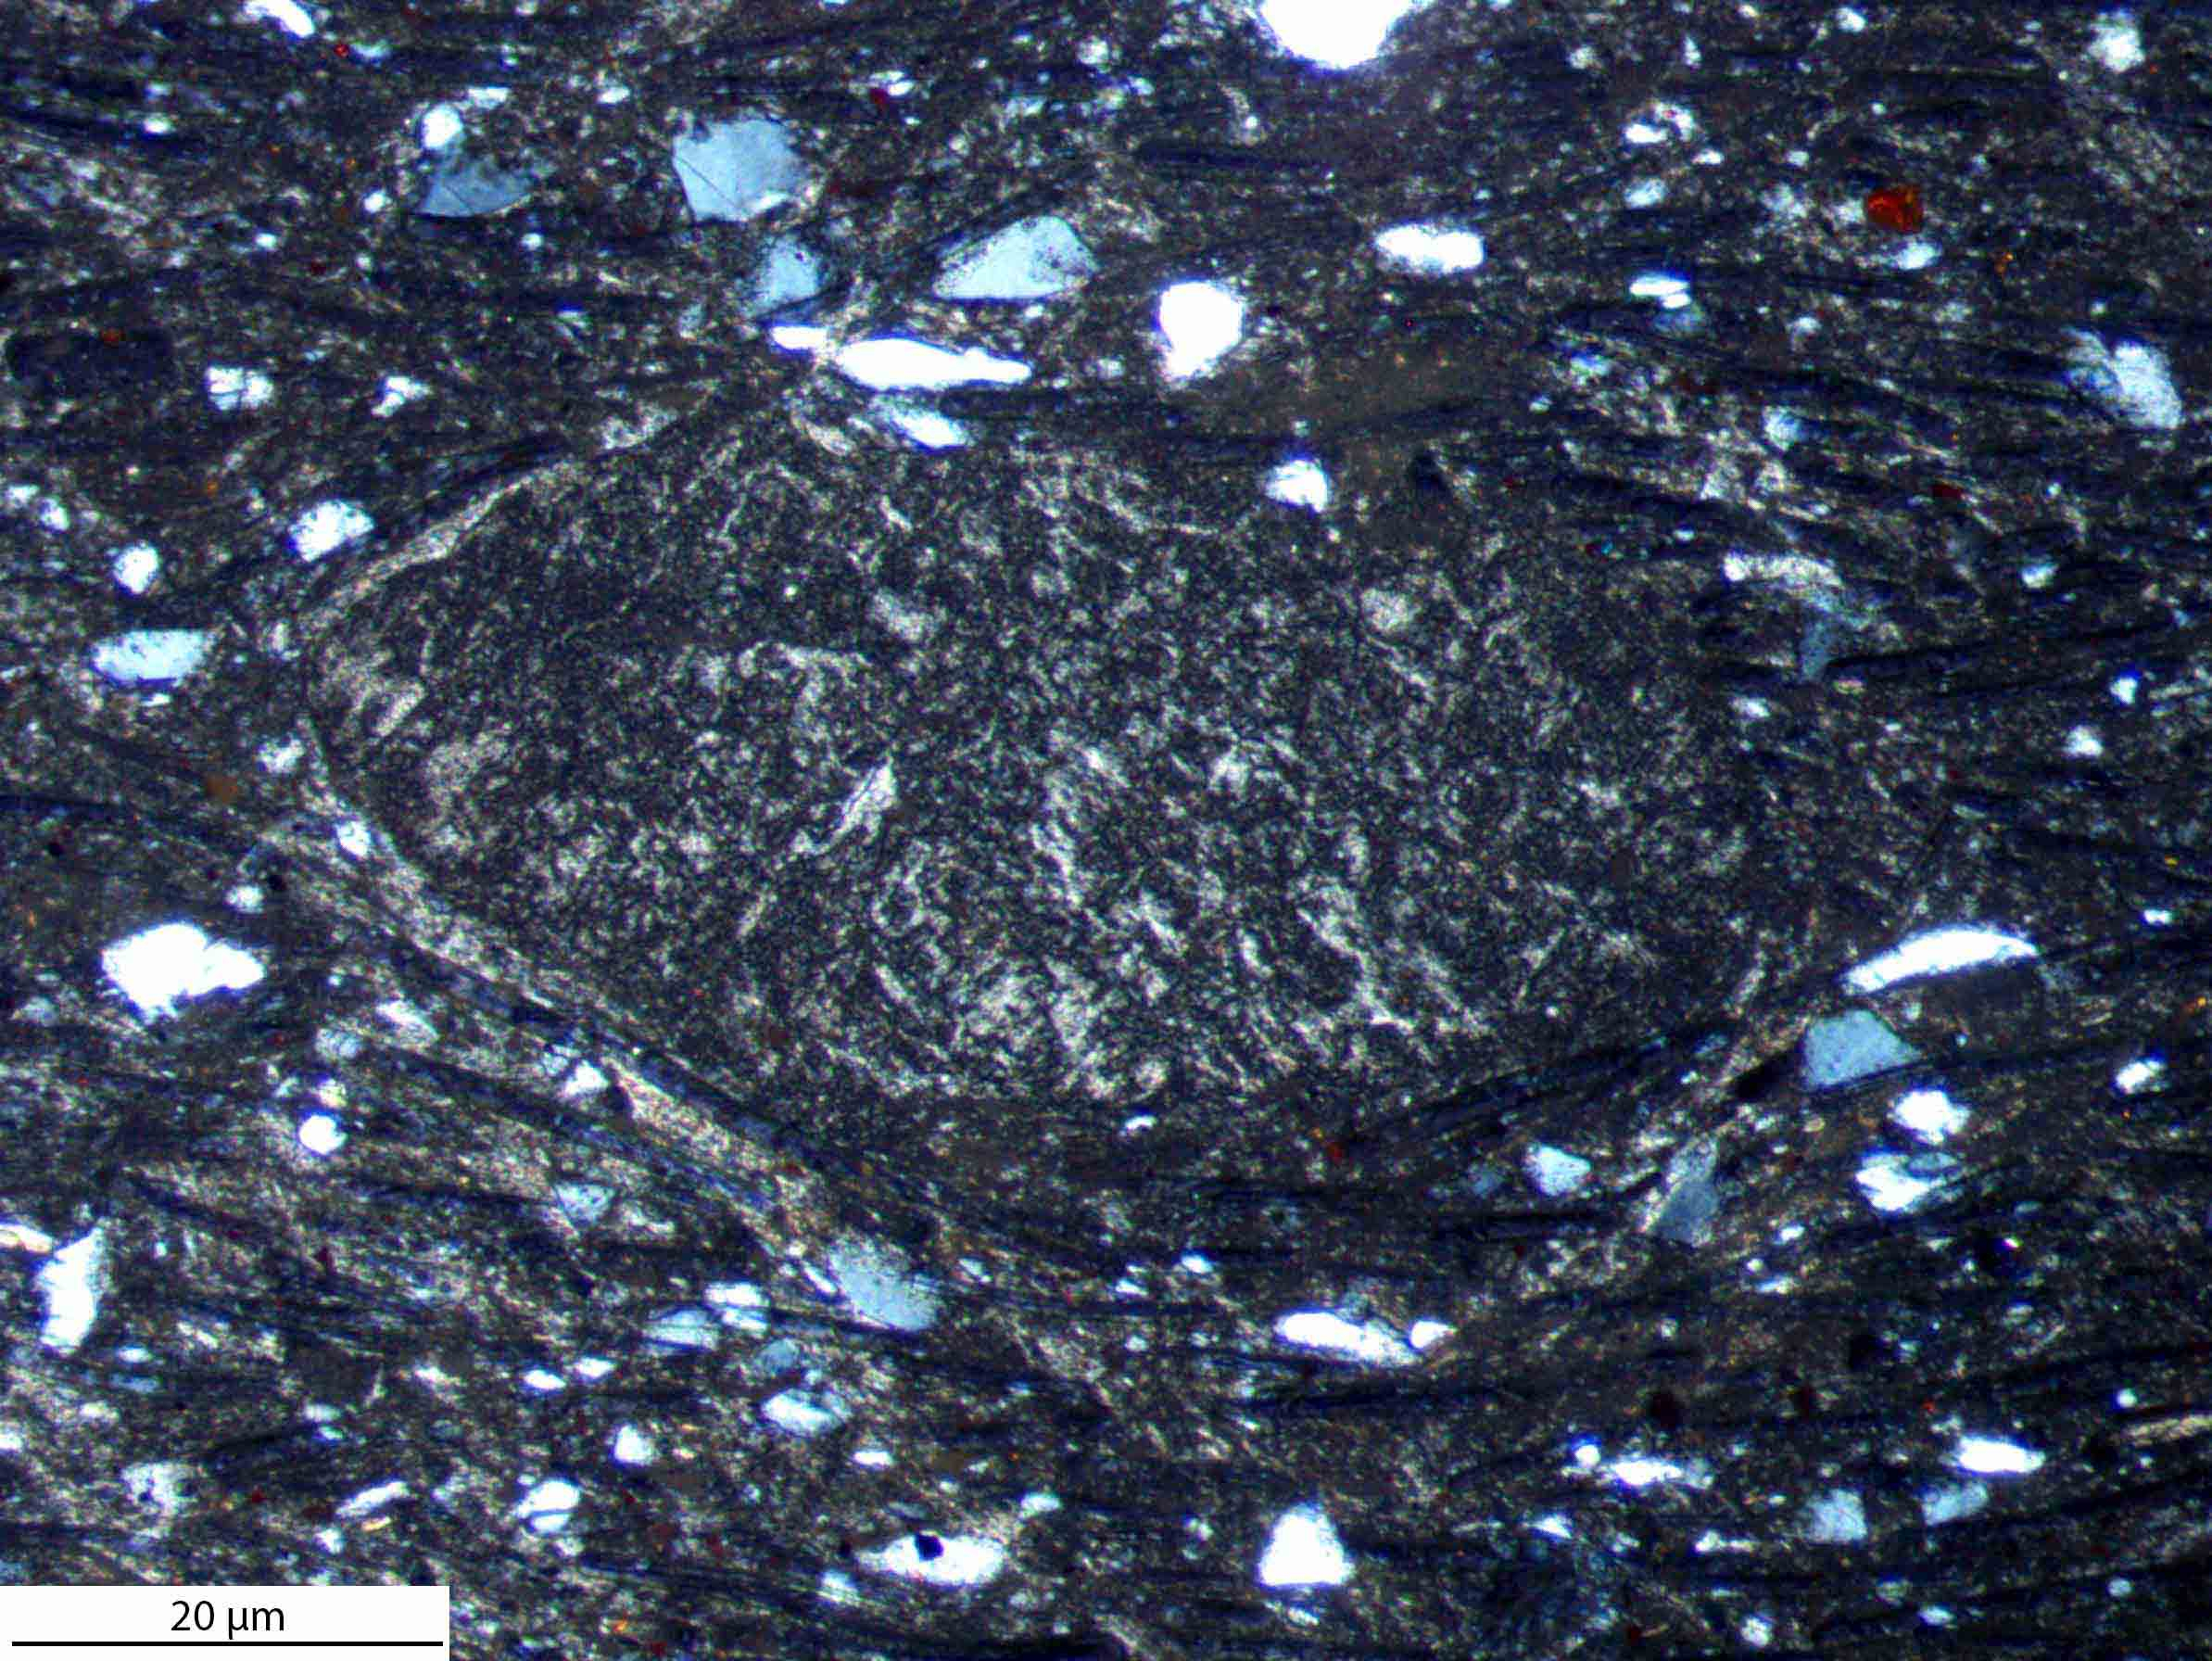
\includegraphics[width=\textwidth]{ThinSections/55_10x_XPL.jpg}
		\caption{Clay pellet [XPL]}
	\end{subfigure}\hspace{.5em}\hfill
%	\begin{subfigure}[t]{.24\textwidth}
%		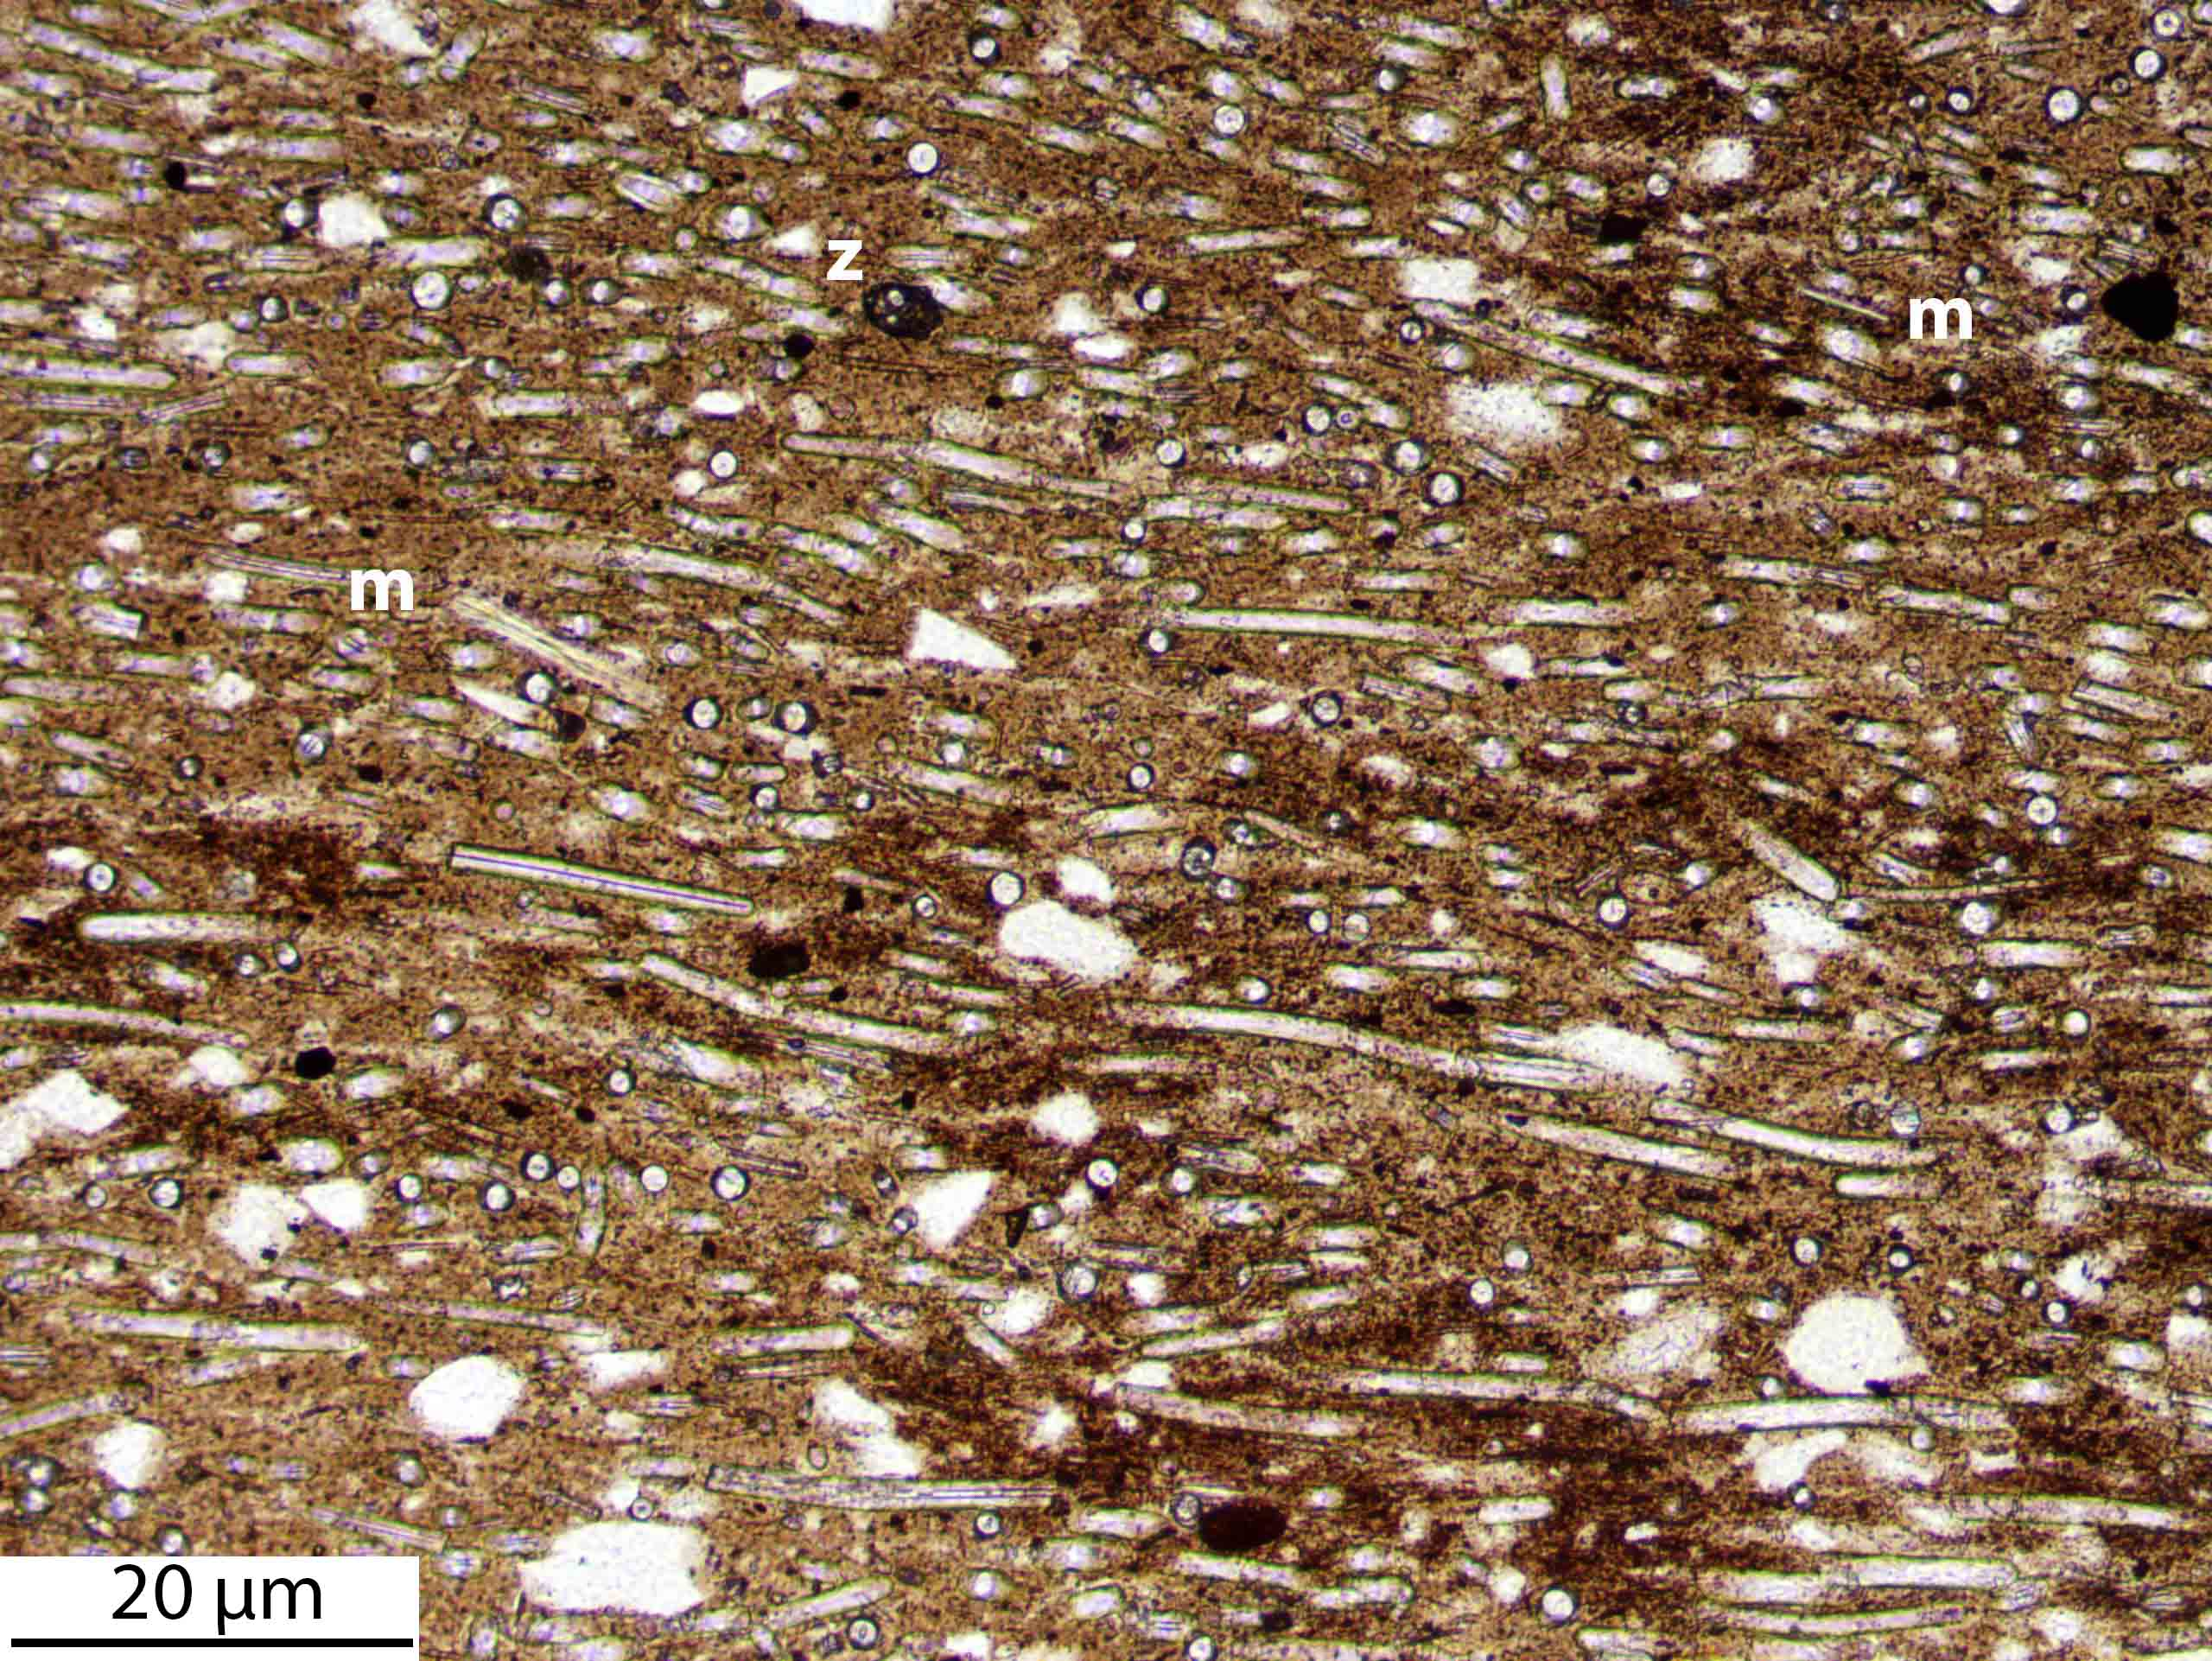
\includegraphics[width=\textwidth]{ThinSections/55-5_10x_PPL.jpg}
%		\caption{Muscovite \& zircon [PPL]}
%	\end{subfigure}\hspace{.1em}\hfill
%	\begin{subfigure}[t]{.24\textwidth}
%		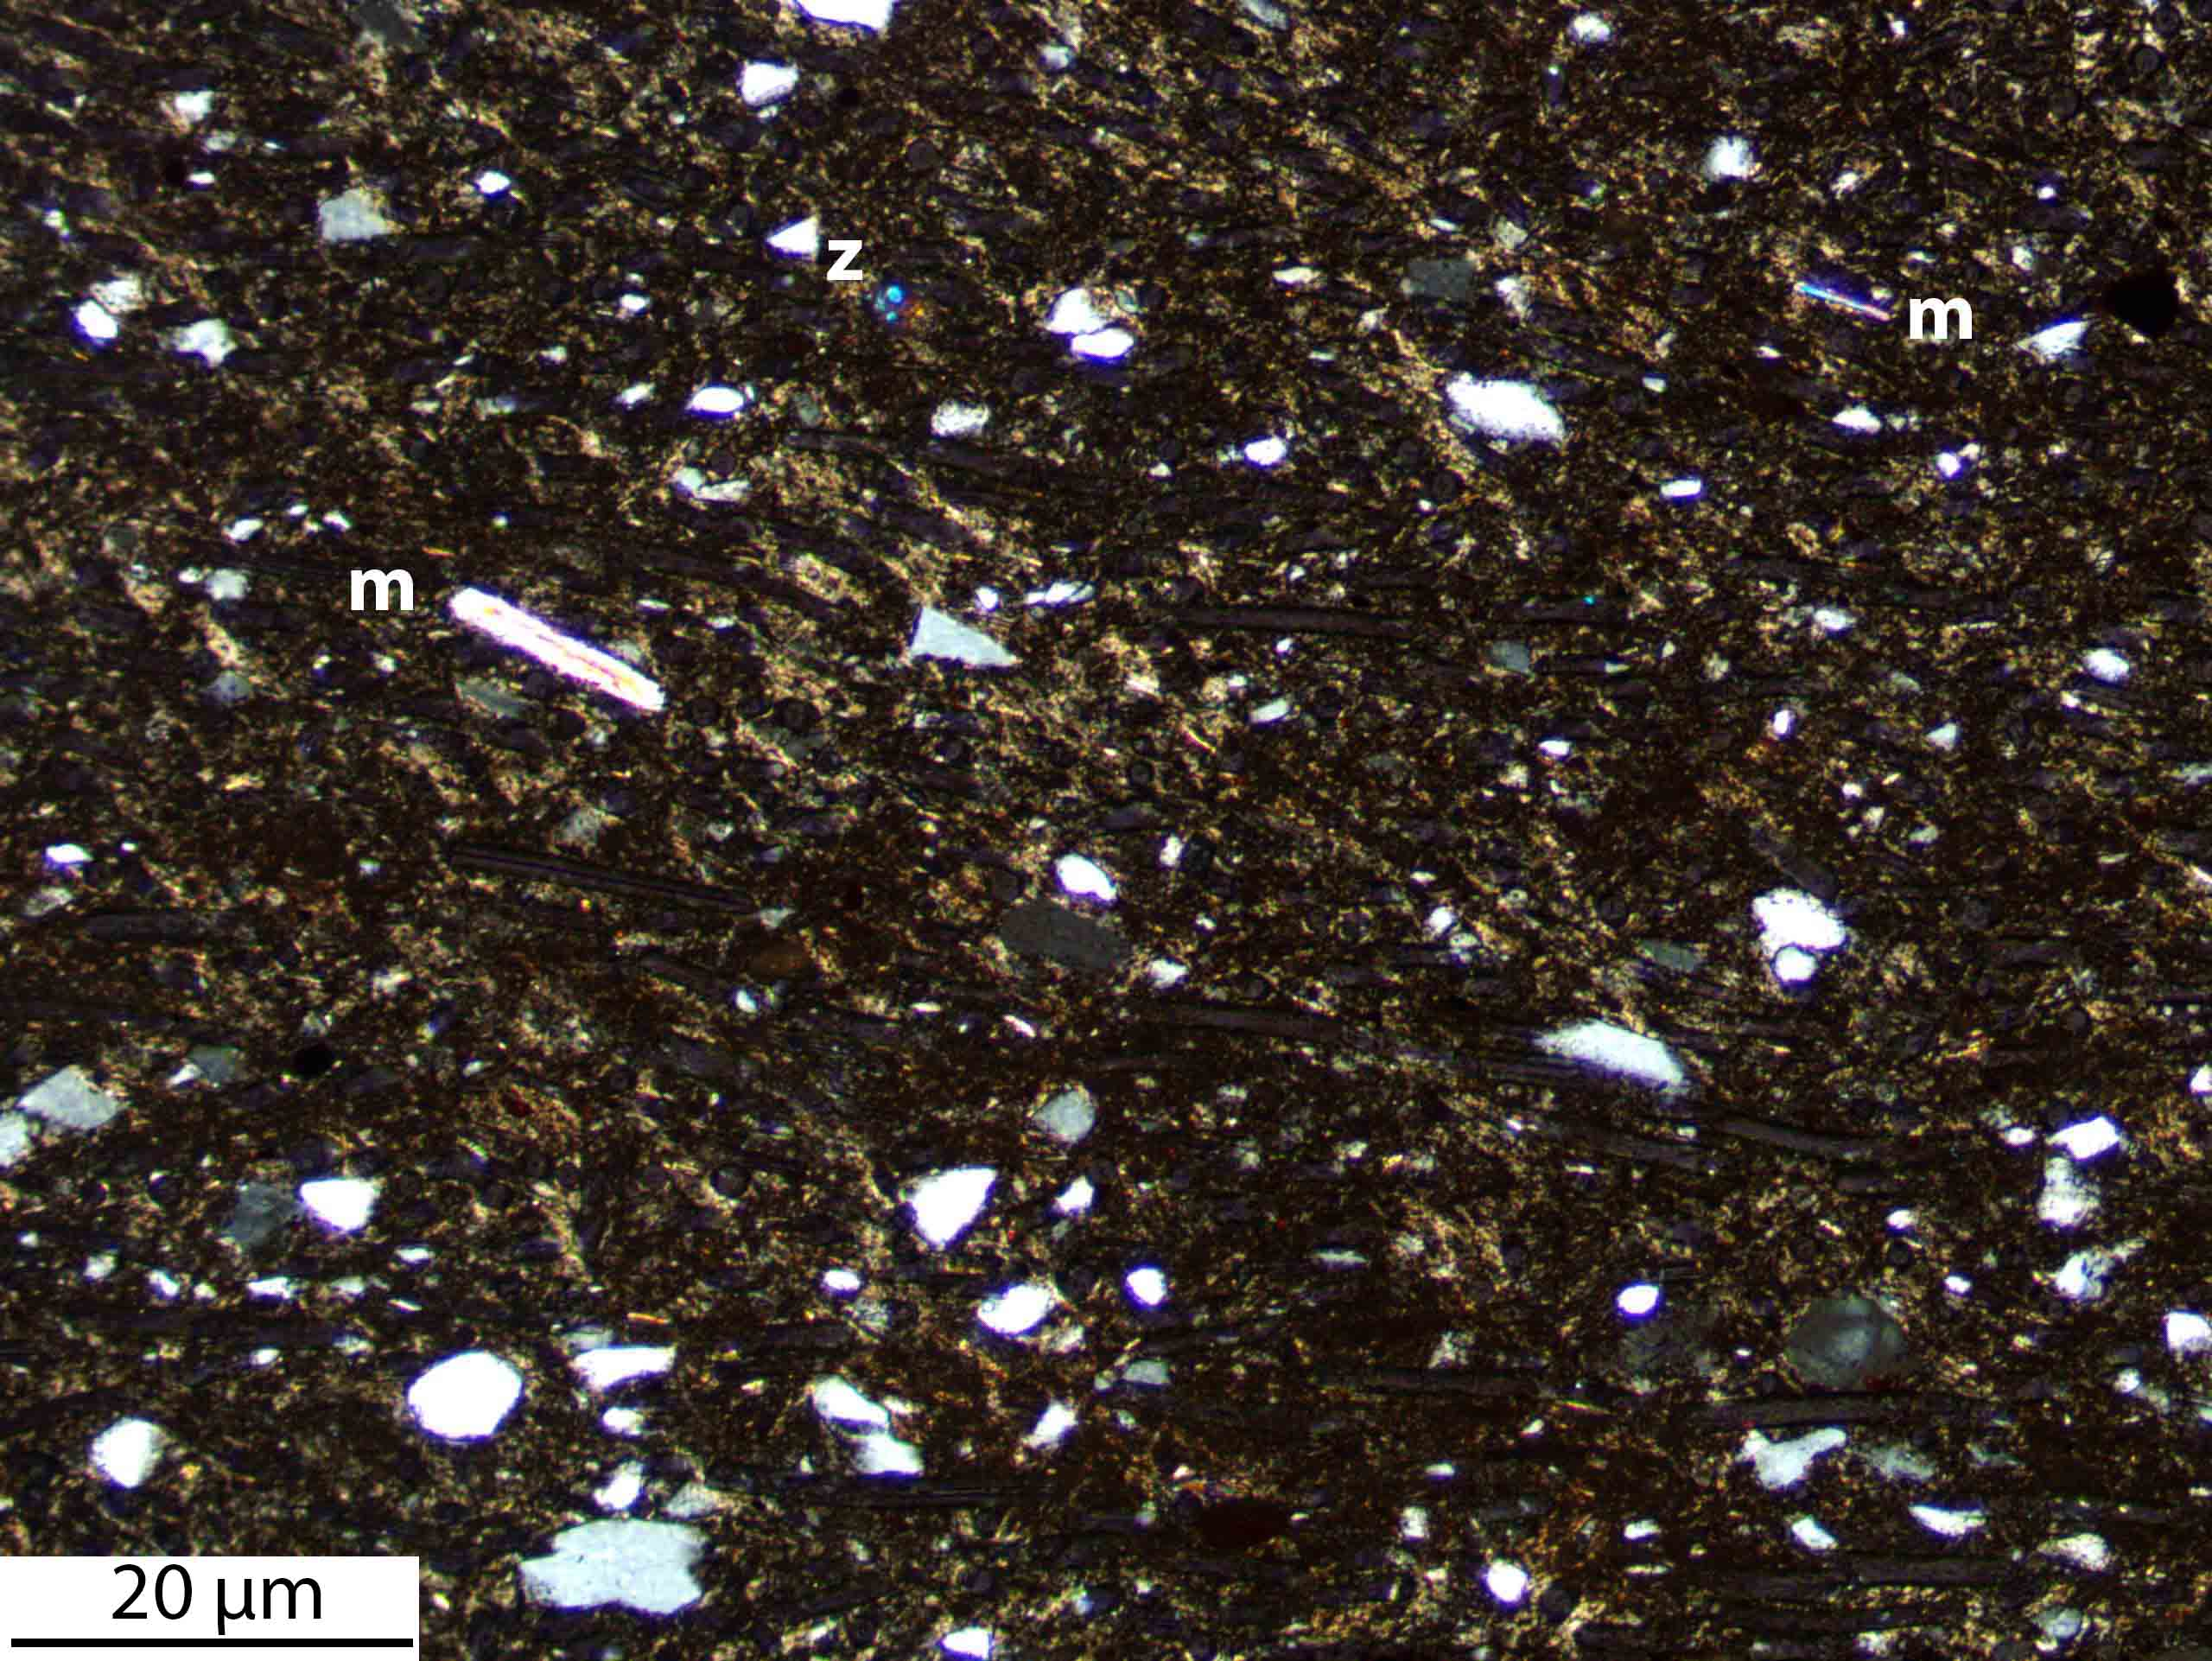
\includegraphics[width=\textwidth]{ThinSections/55-5_10x_XPL.jpg}
%		\caption{Muscovite \& zircon [XPL]}
%	\end{subfigure}\hspace{.5em}\hfill
%	\begin{subfigure}[t]{.24\textwidth}
%		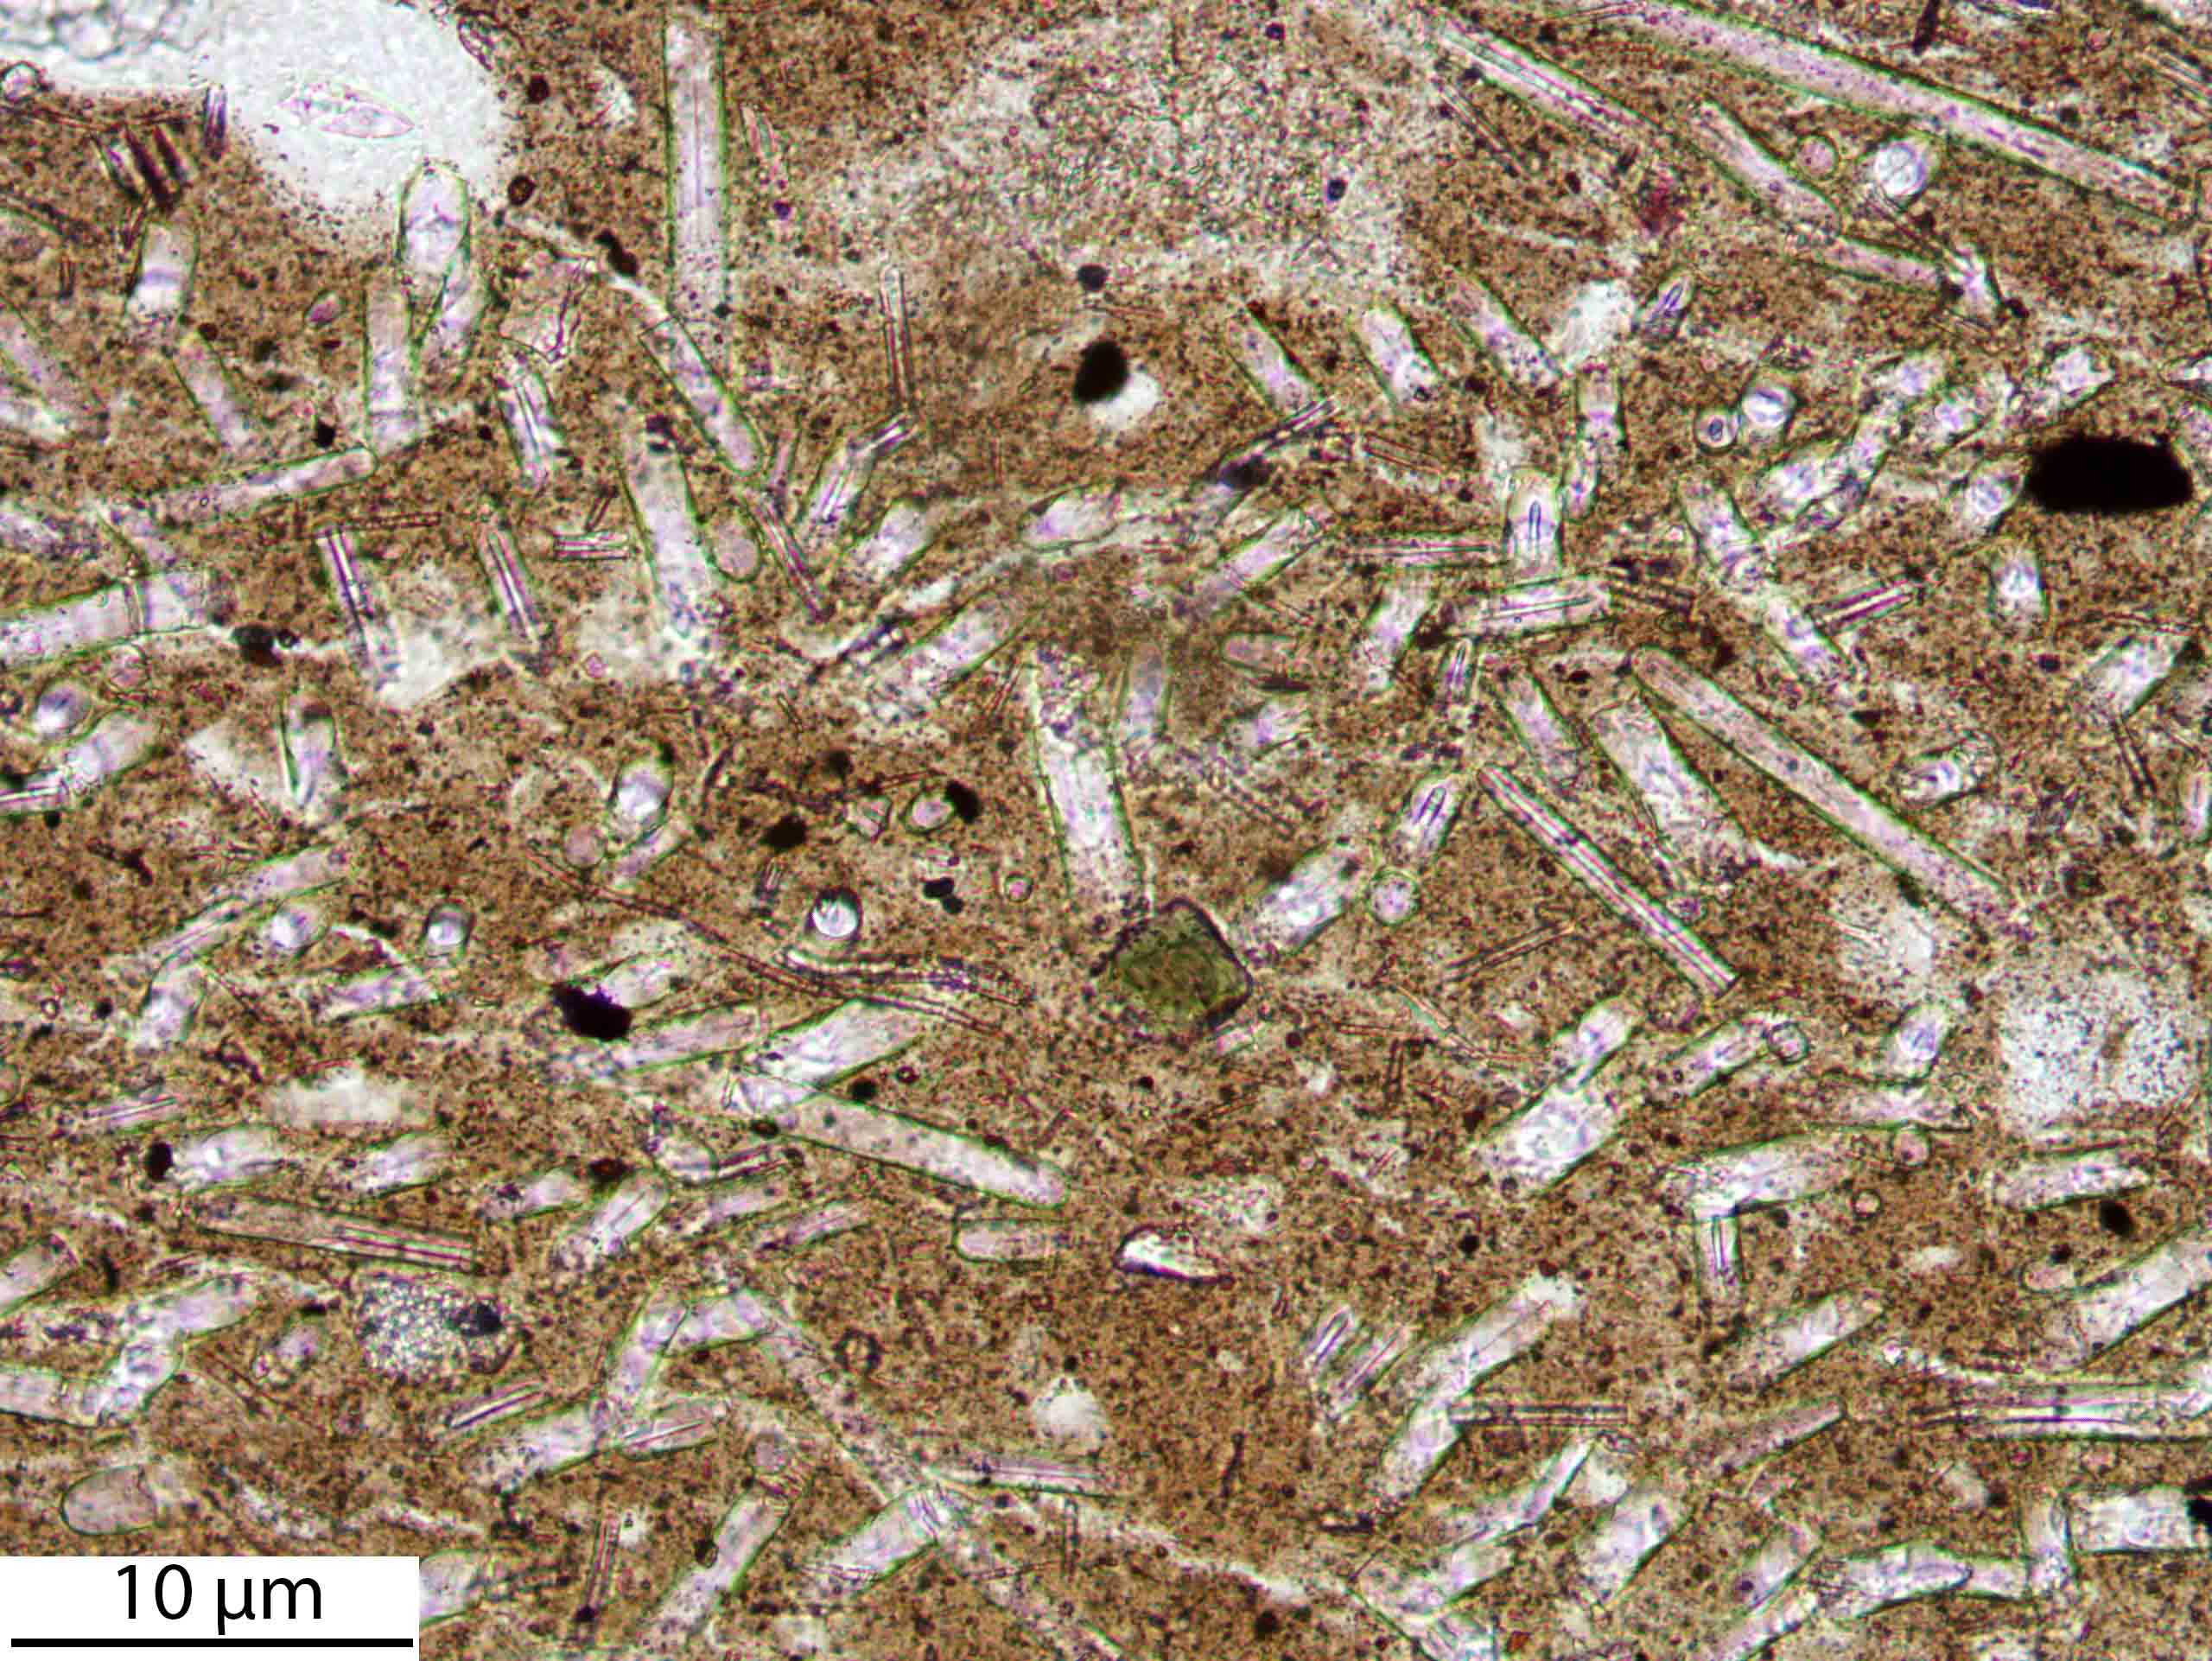
\includegraphics[width=\textwidth]{ThinSections/55-3_20x_PPL.jpg}
%		\caption{Tourmaline [PPL]}
%	\end{subfigure}\hspace{.1em}\hfill
%	\begin{subfigure}[t]{.24\textwidth}
%		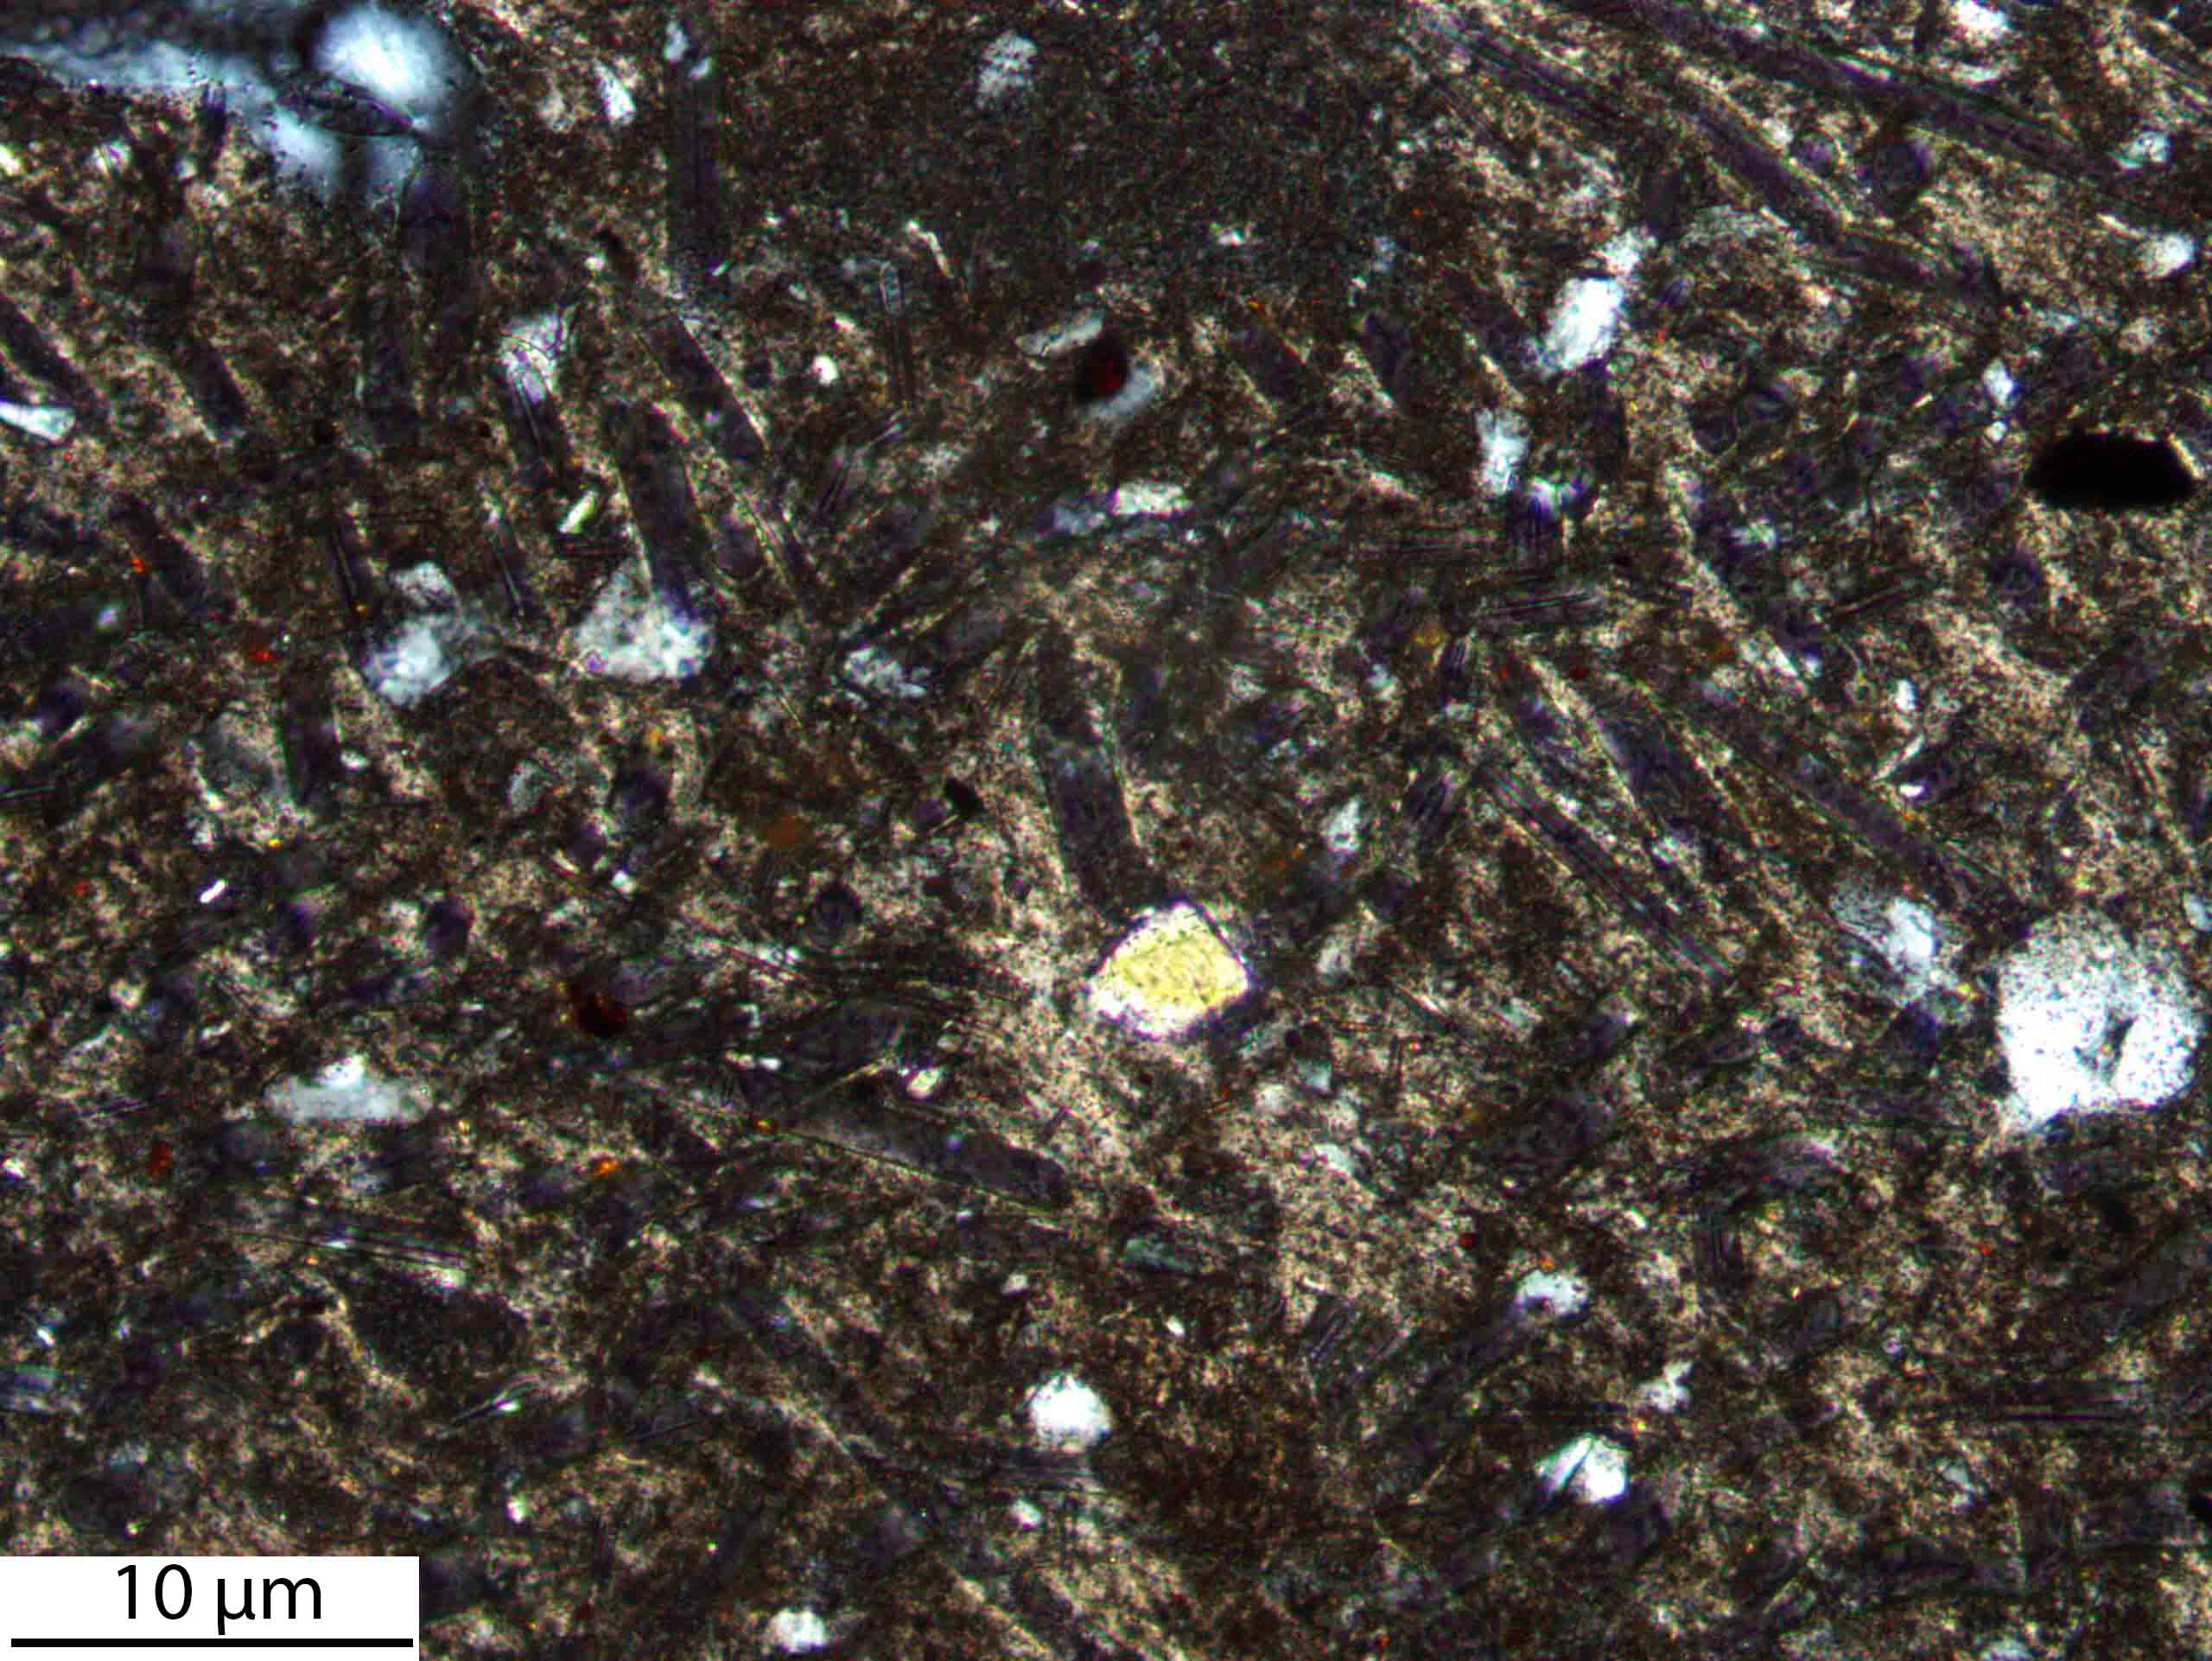
\includegraphics[width=\textwidth]{ThinSections/55-3_20x_XPL.jpg}
%		\caption{Tourmaline [XPL]}
%	\end{subfigure}\hfill
	\caption{}
	\label{fig:55_pik}
\end{figure}

\newpage\subsection{PIK 87/1-2:123 (pik\#10; Mandombe style)}

\begin{multicols}{2}
\noindent The fine fraction is homogeneous and non-calcareous (light yellowish to dark brown [PPL]) with stipple speckled b-fabric. Voids show no orientation. The coarse-fraction consists mainly of sub-angular quartz in clear bimodal grain-size distribution, including a high proportion of runiquartz. Common are sub-rounded iron rich (dark reddish [PPL]) heterogeneous clay pellets. Occasionally present are muscovite and biotite as well as charred plant matter, plagioclase and zircon. The c/f-related distribution pattern is single-spaced porphyric.
\end{multicols}

% FM: hornblende or tourmaline (strangly cut)
% Less common are sub-angular homogeneous clay pellet

%\vfill
\begin{figure}[H]
	\centering
	\begin{subfigure}[t]{.49\textwidth}
		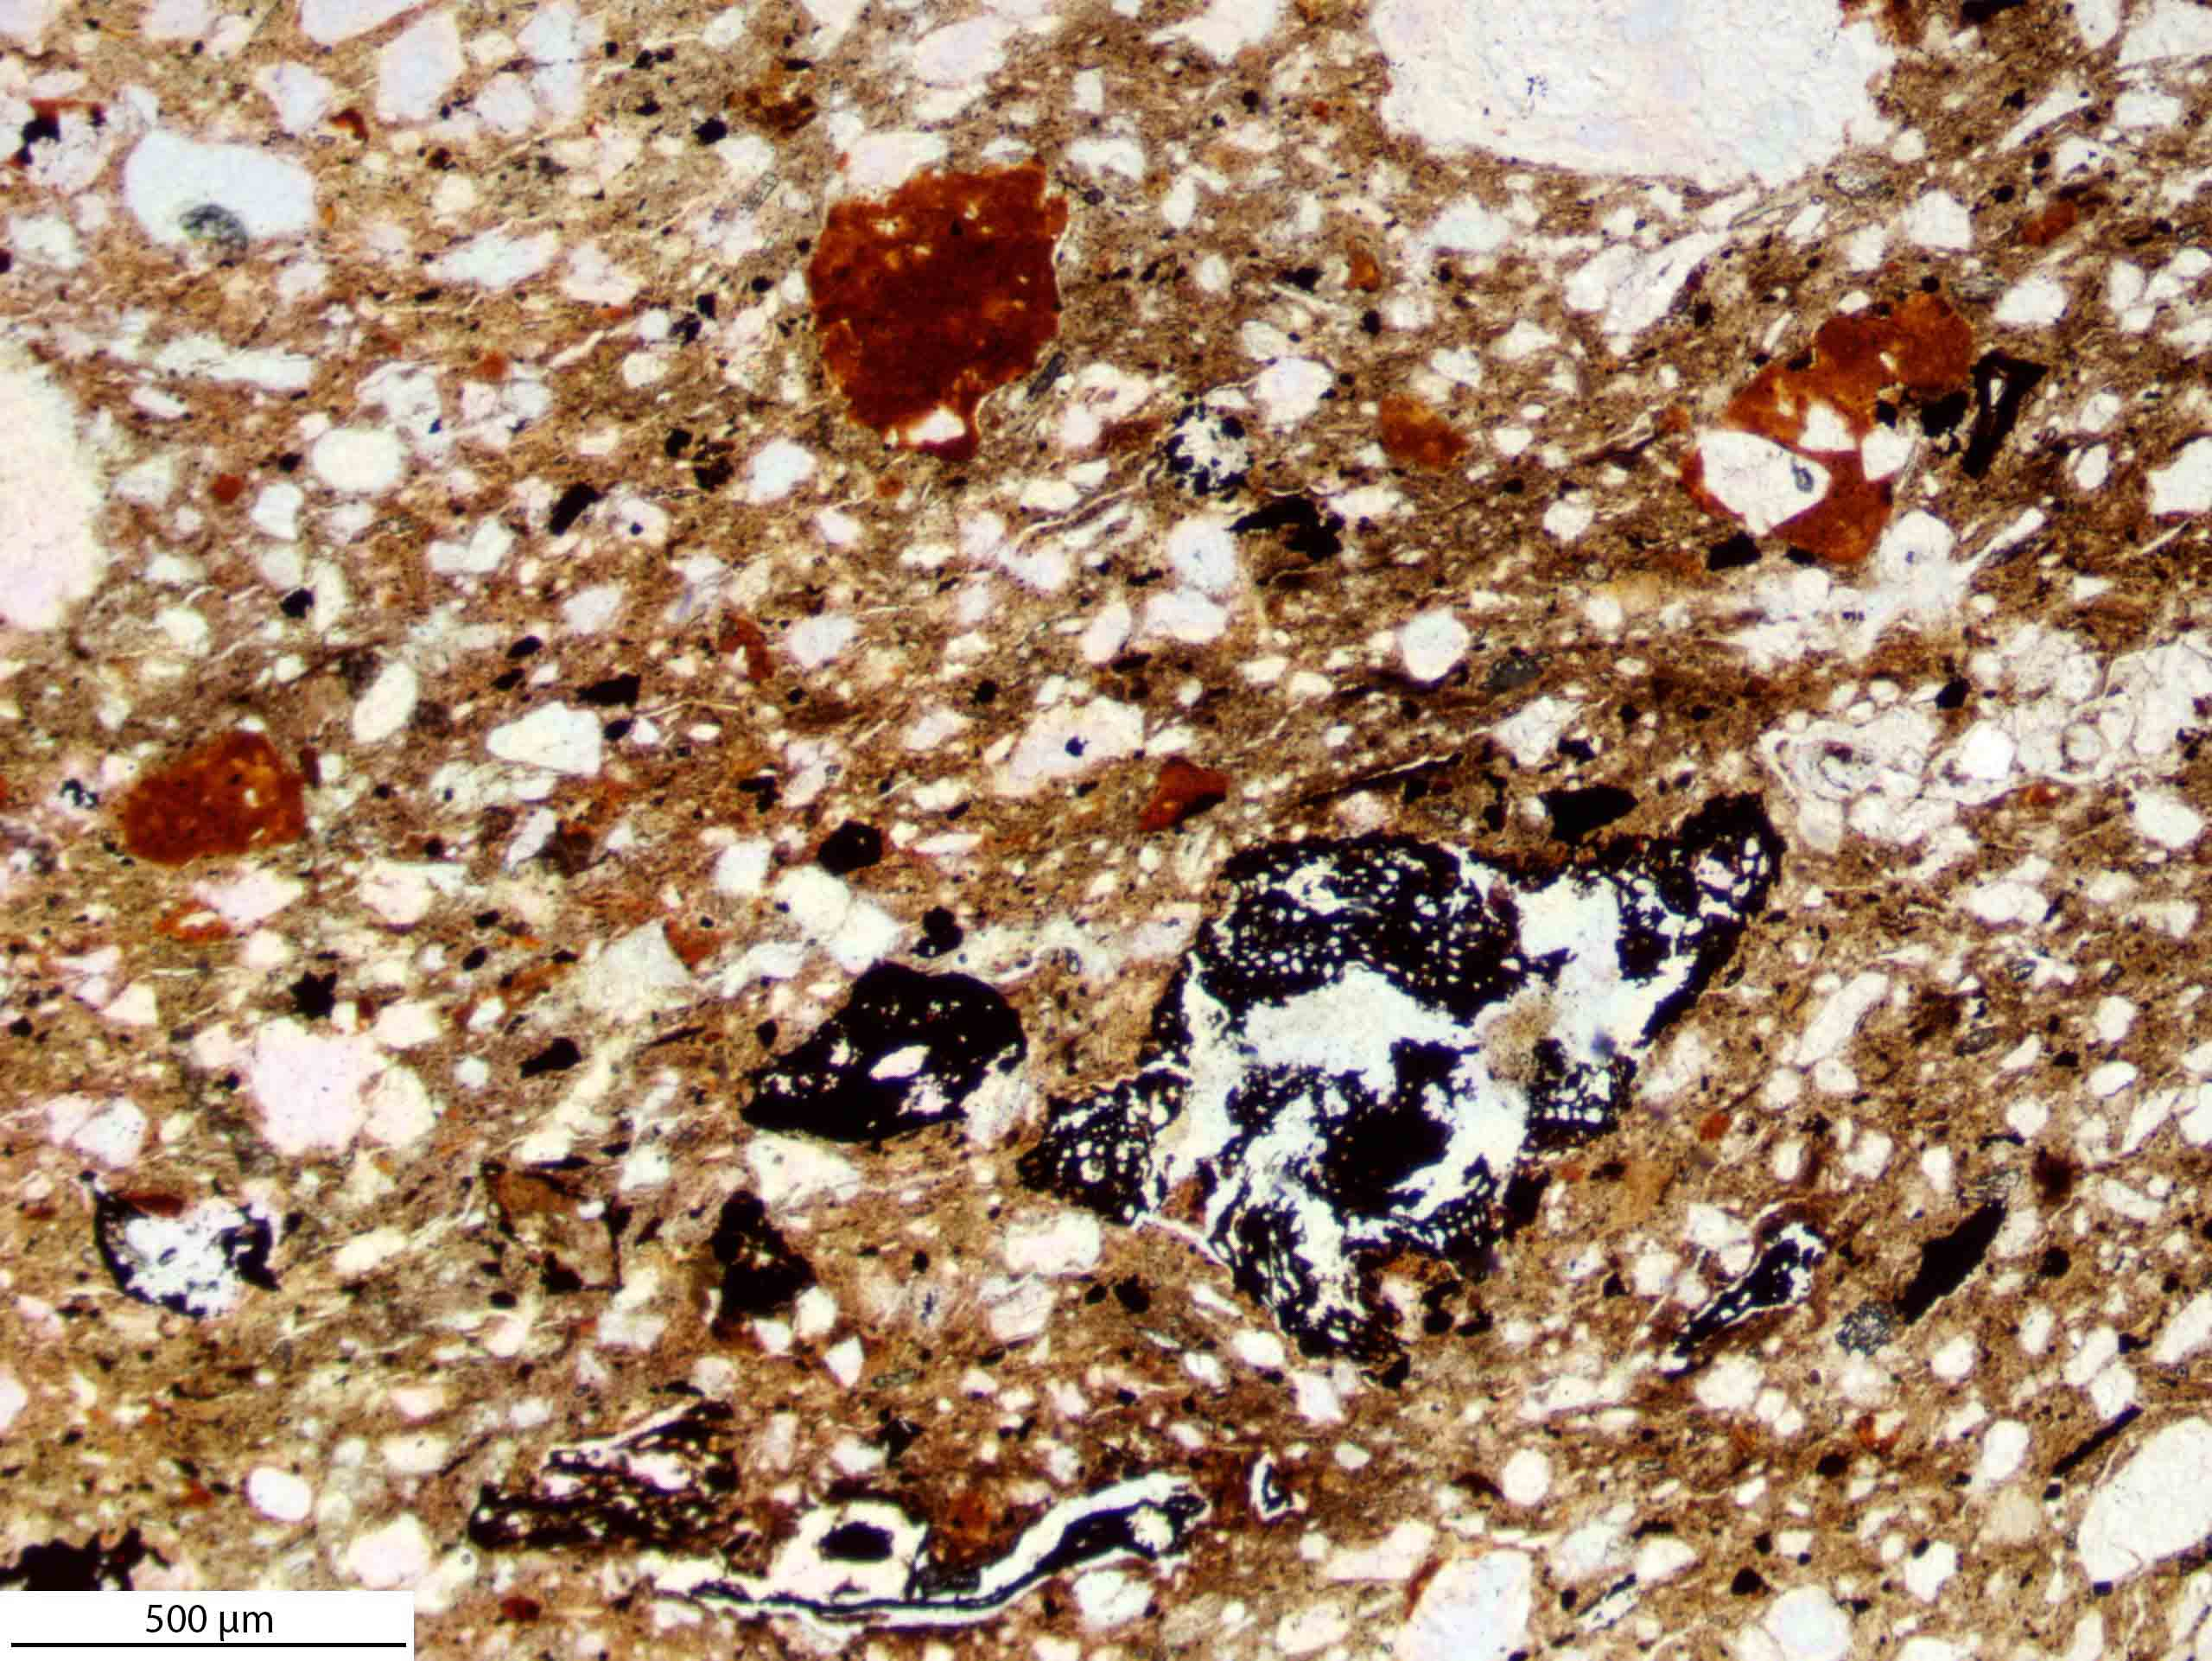
\includegraphics[width=\textwidth]{ThinSections/10-8_4x_PPL.jpg}
		\caption{[PPL]}
	\end{subfigure}\hspace{.5em}\hfill
	\begin{subfigure}[t]{.49\textwidth}
		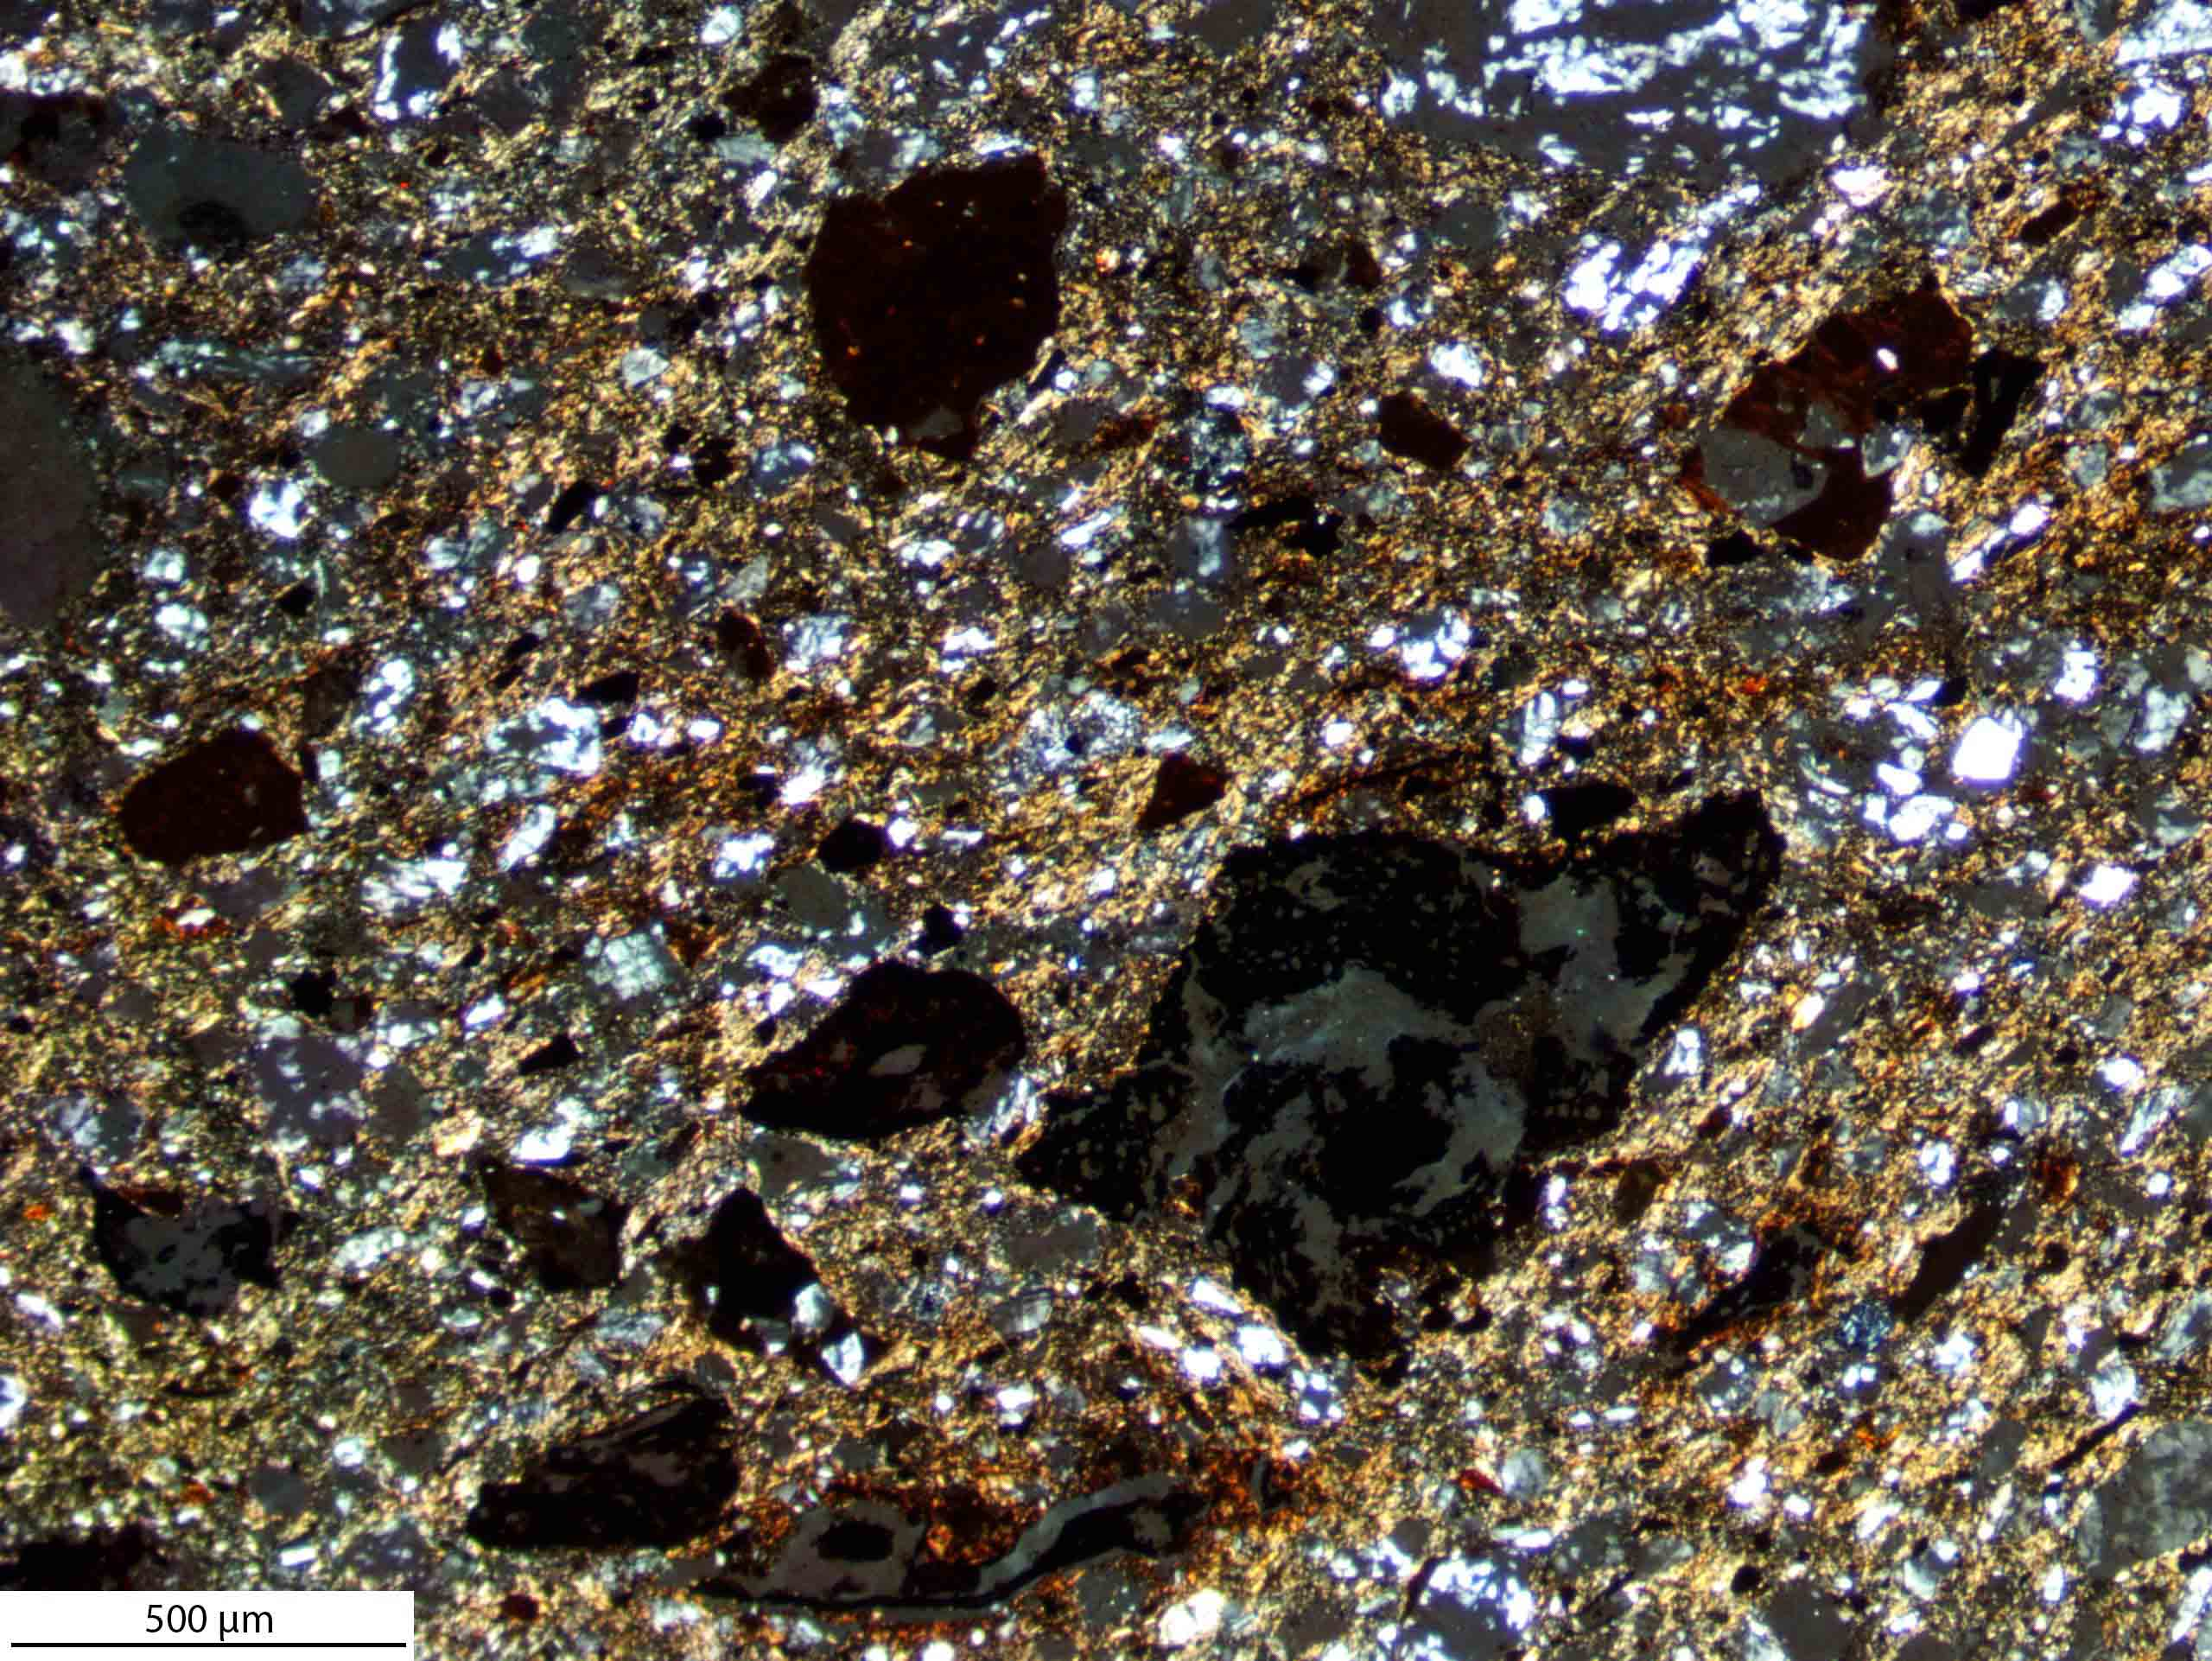
\includegraphics[width=\textwidth]{ThinSections/10-8_4x_XPL.jpg}
		\caption{[XPL]}
	\end{subfigure}
	\begin{subfigure}[t]{.32\textwidth}
		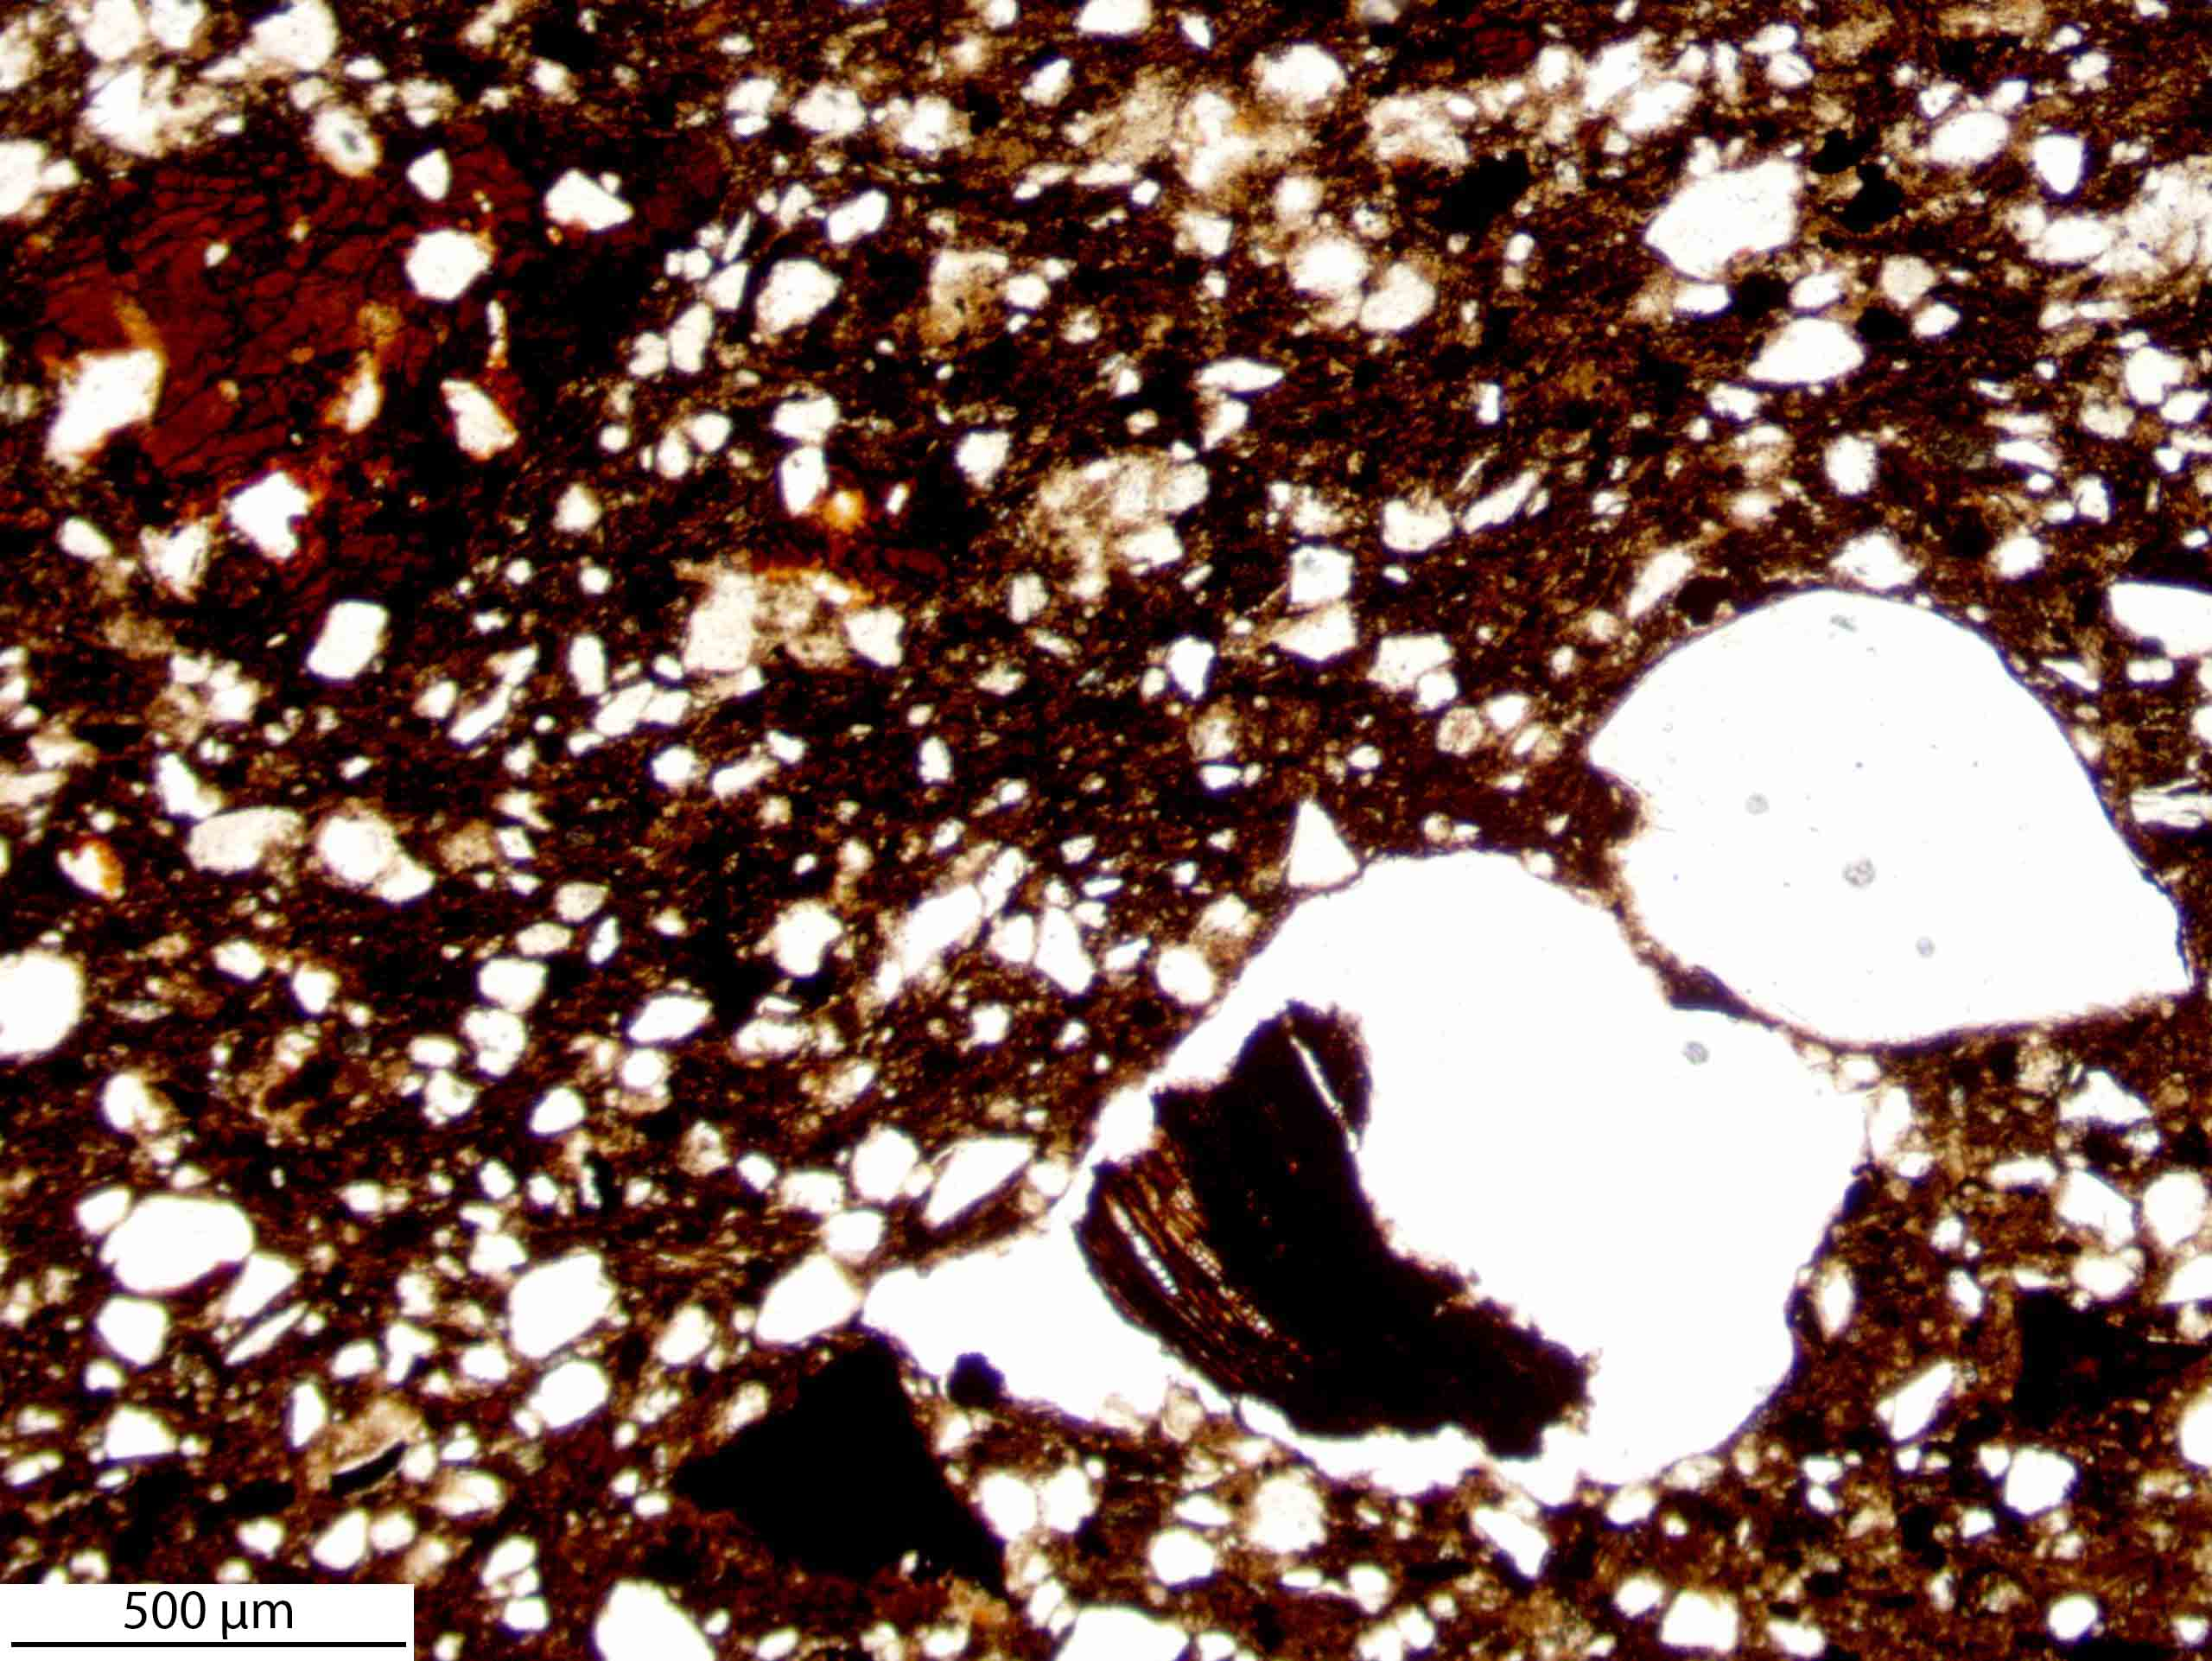
\includegraphics[width=\textwidth]{ThinSections/10-2_4x_PPL.jpg}
		\caption{Clay pellet \& plant matter [PPL]}
	\end{subfigure}\hspace{.1em}\hfill
%	\begin{subfigure}[t]{.32\textwidth}
%		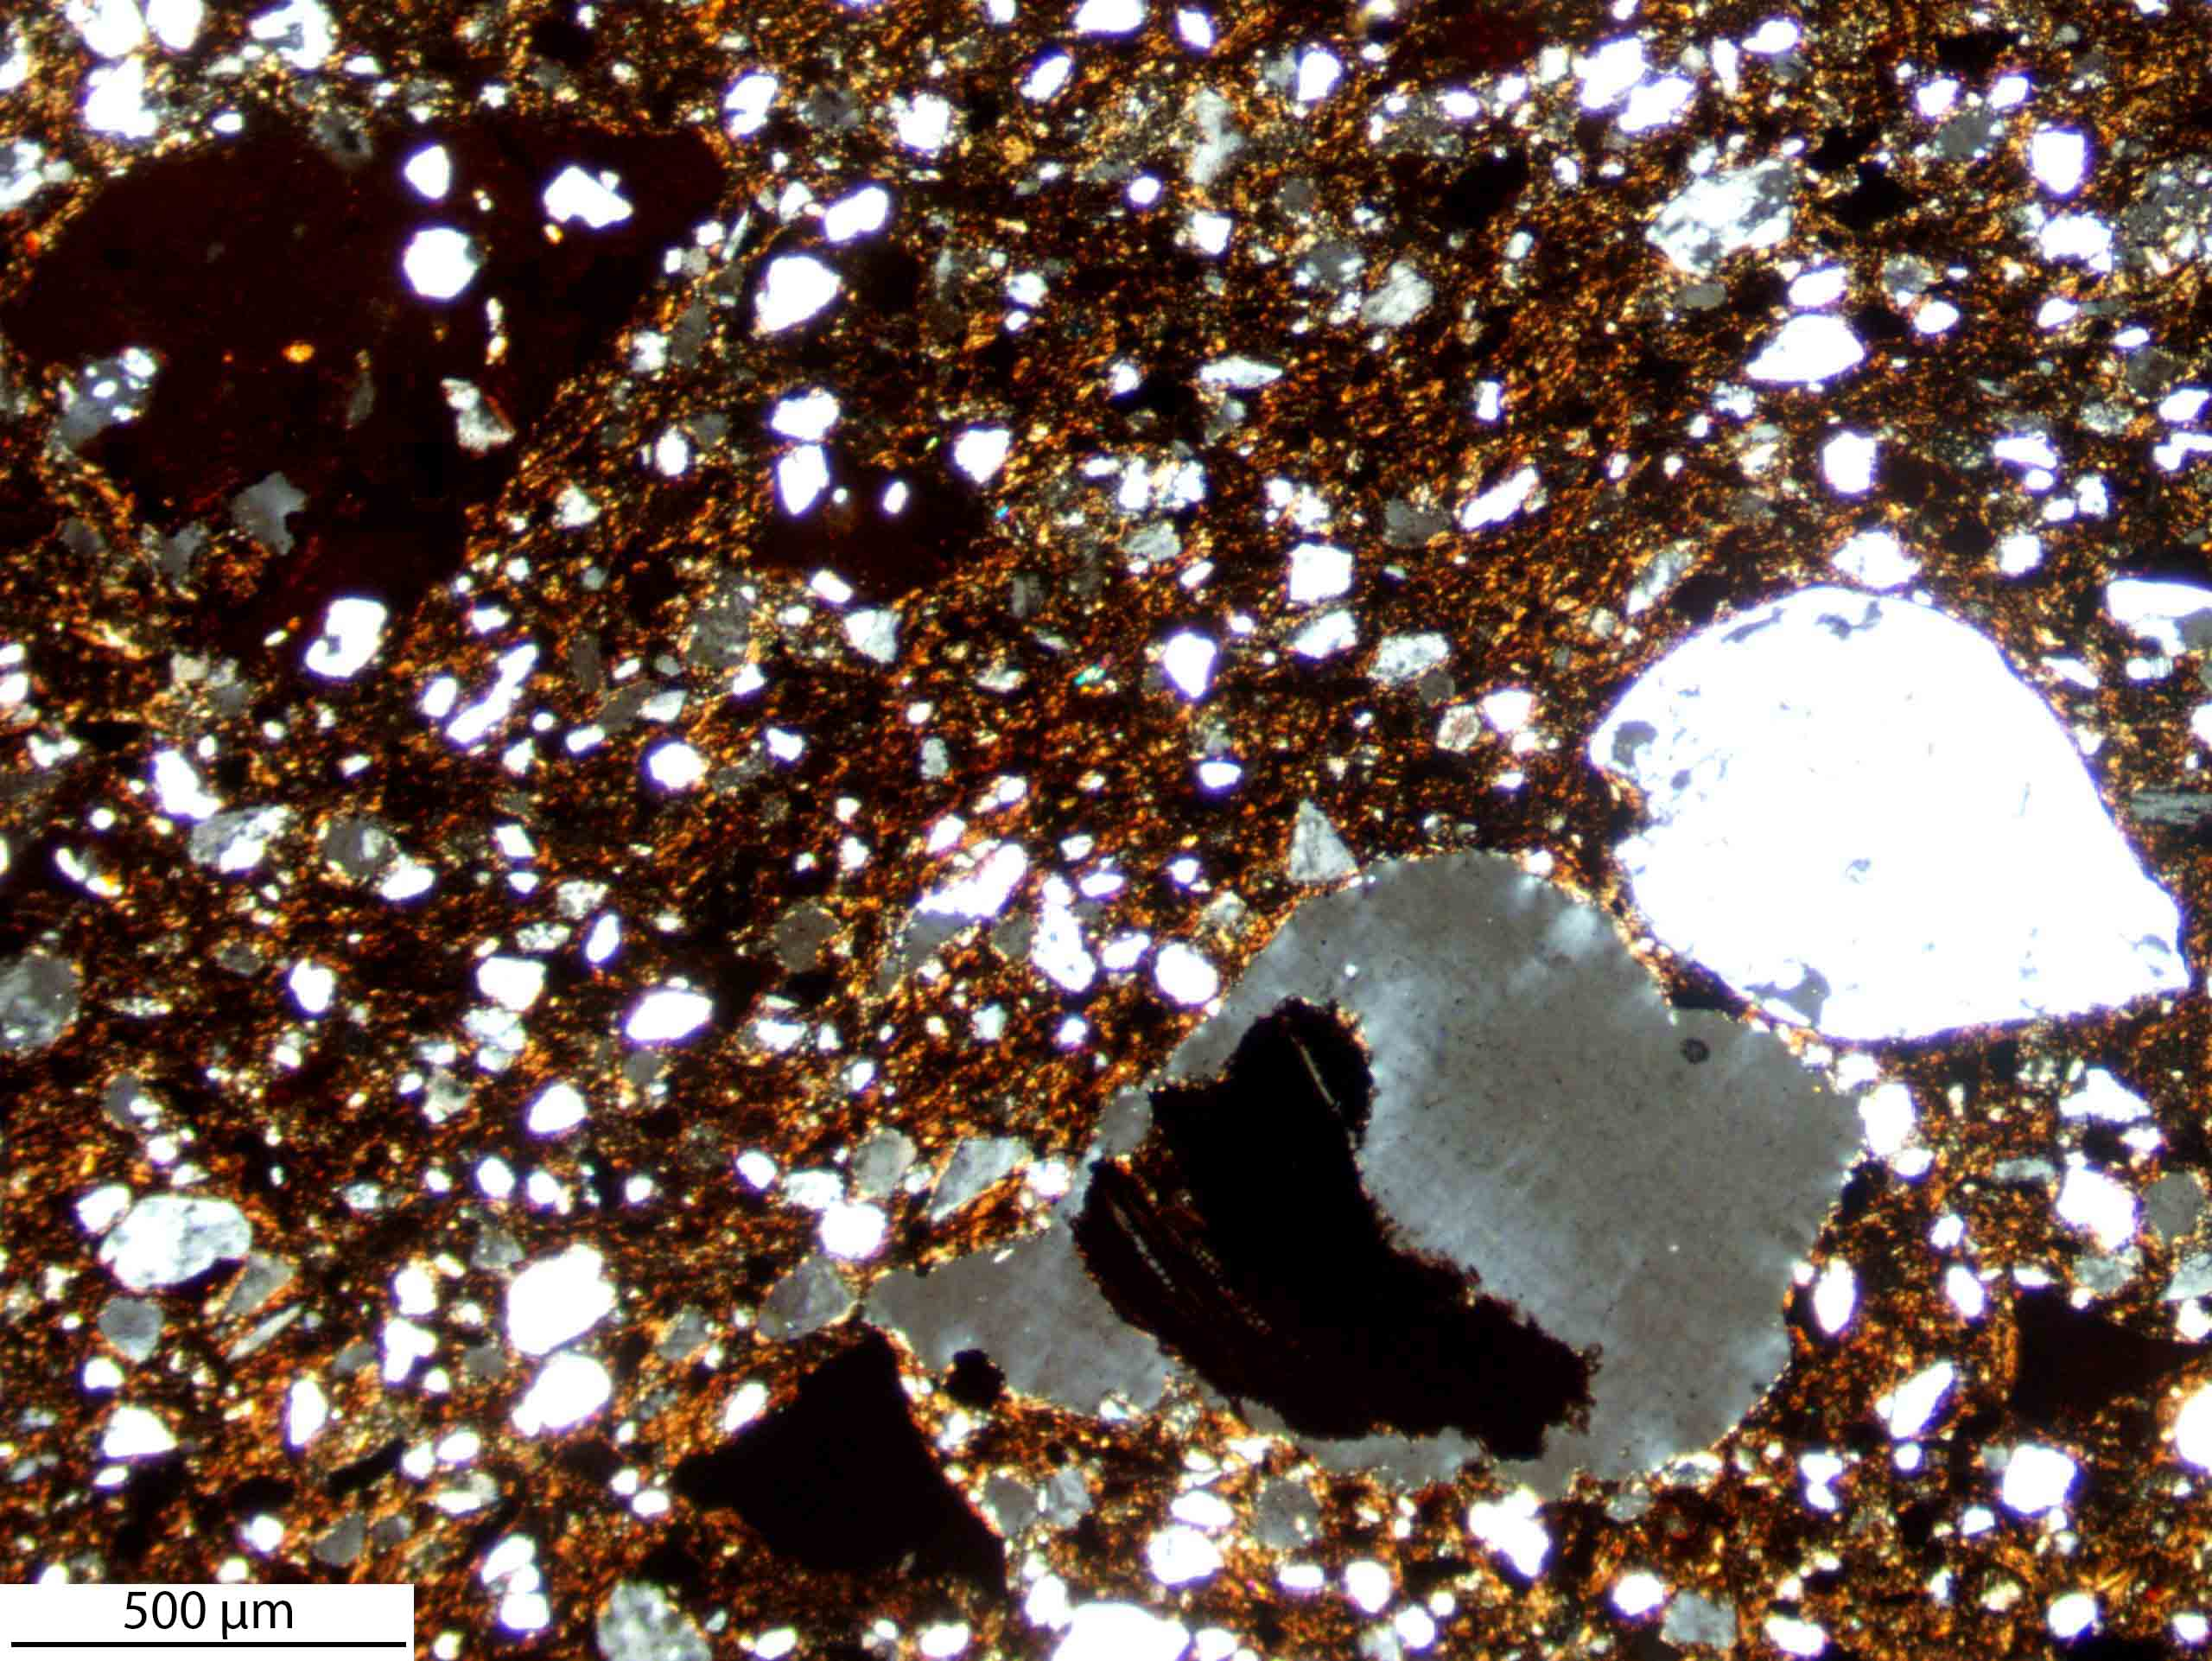
\includegraphics[width=\textwidth]{ThinSections/10-2_4x_XPL.jpg}
%		\caption{Clay pellet \& plant matter [XPL]}
%	\end{subfigure}\hspace{.1em}\hfill
	\begin{subfigure}[t]{.32\textwidth}
		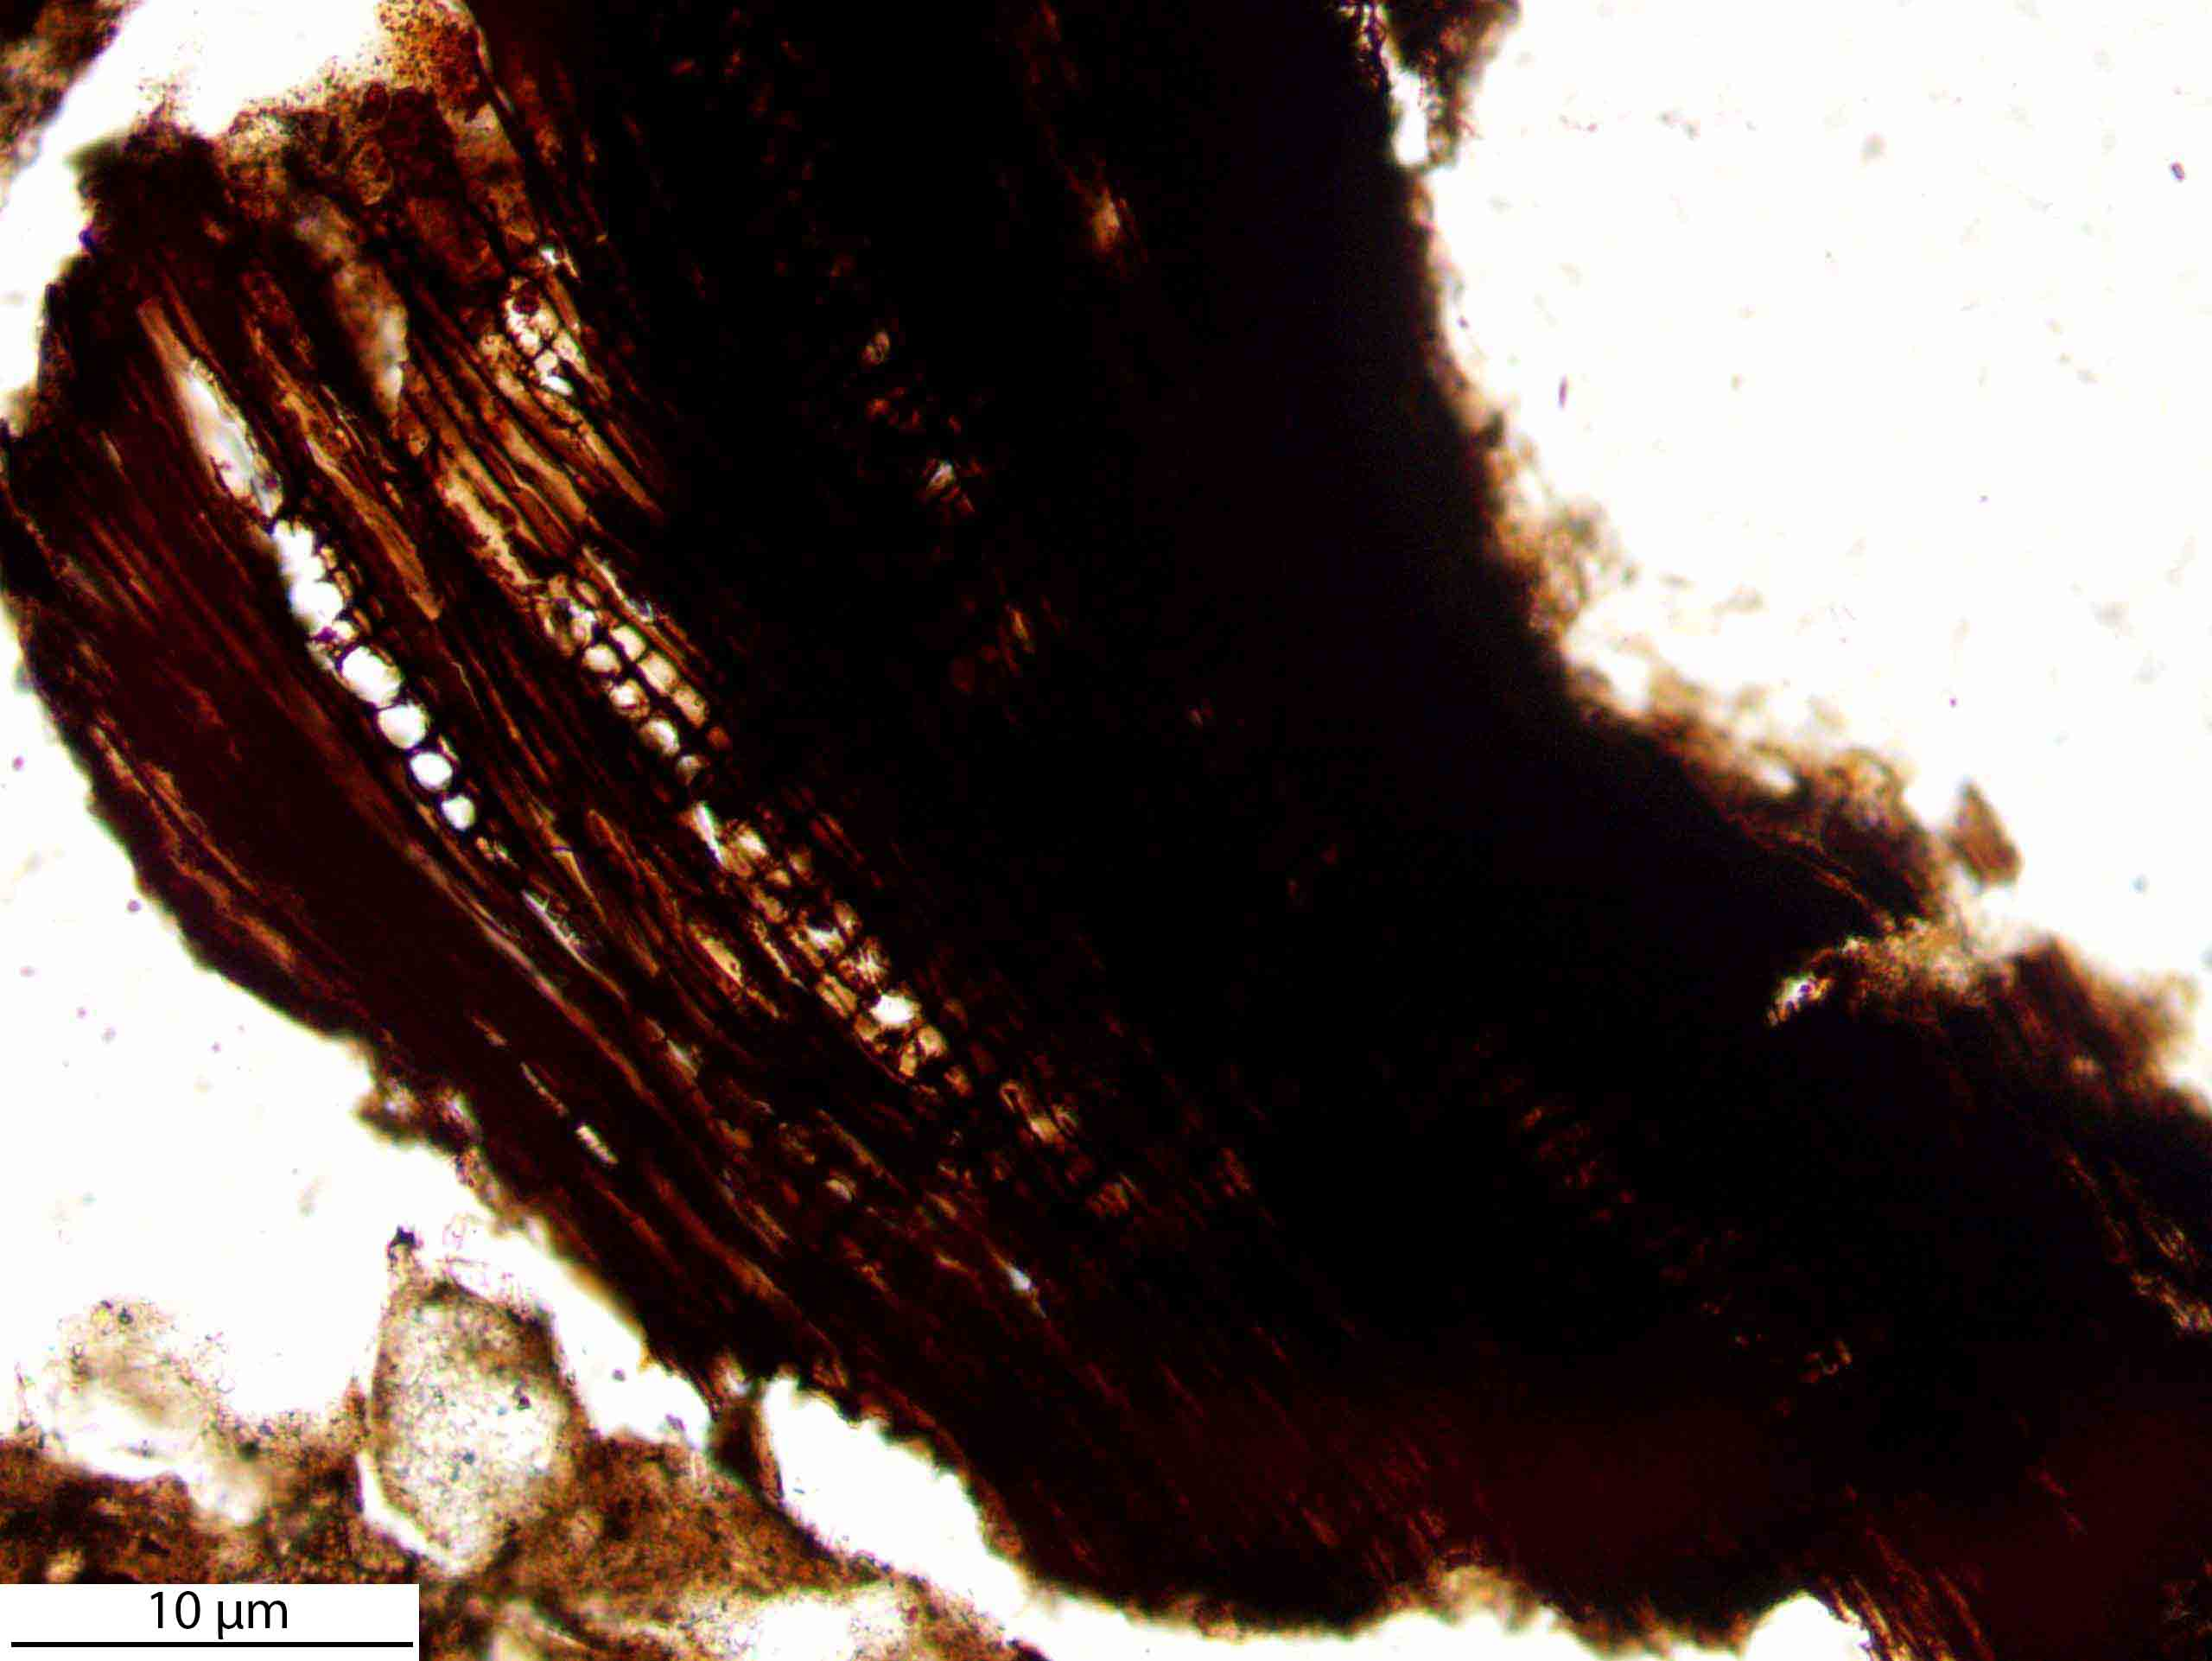
\includegraphics[width=\textwidth]{ThinSections/10-2_20x_PPL.jpg}
		\caption{Detail plant matter [PPL]}
	\end{subfigure}\hspace{.1em}\hfill
	\begin{subfigure}[t]{.32\textwidth}
		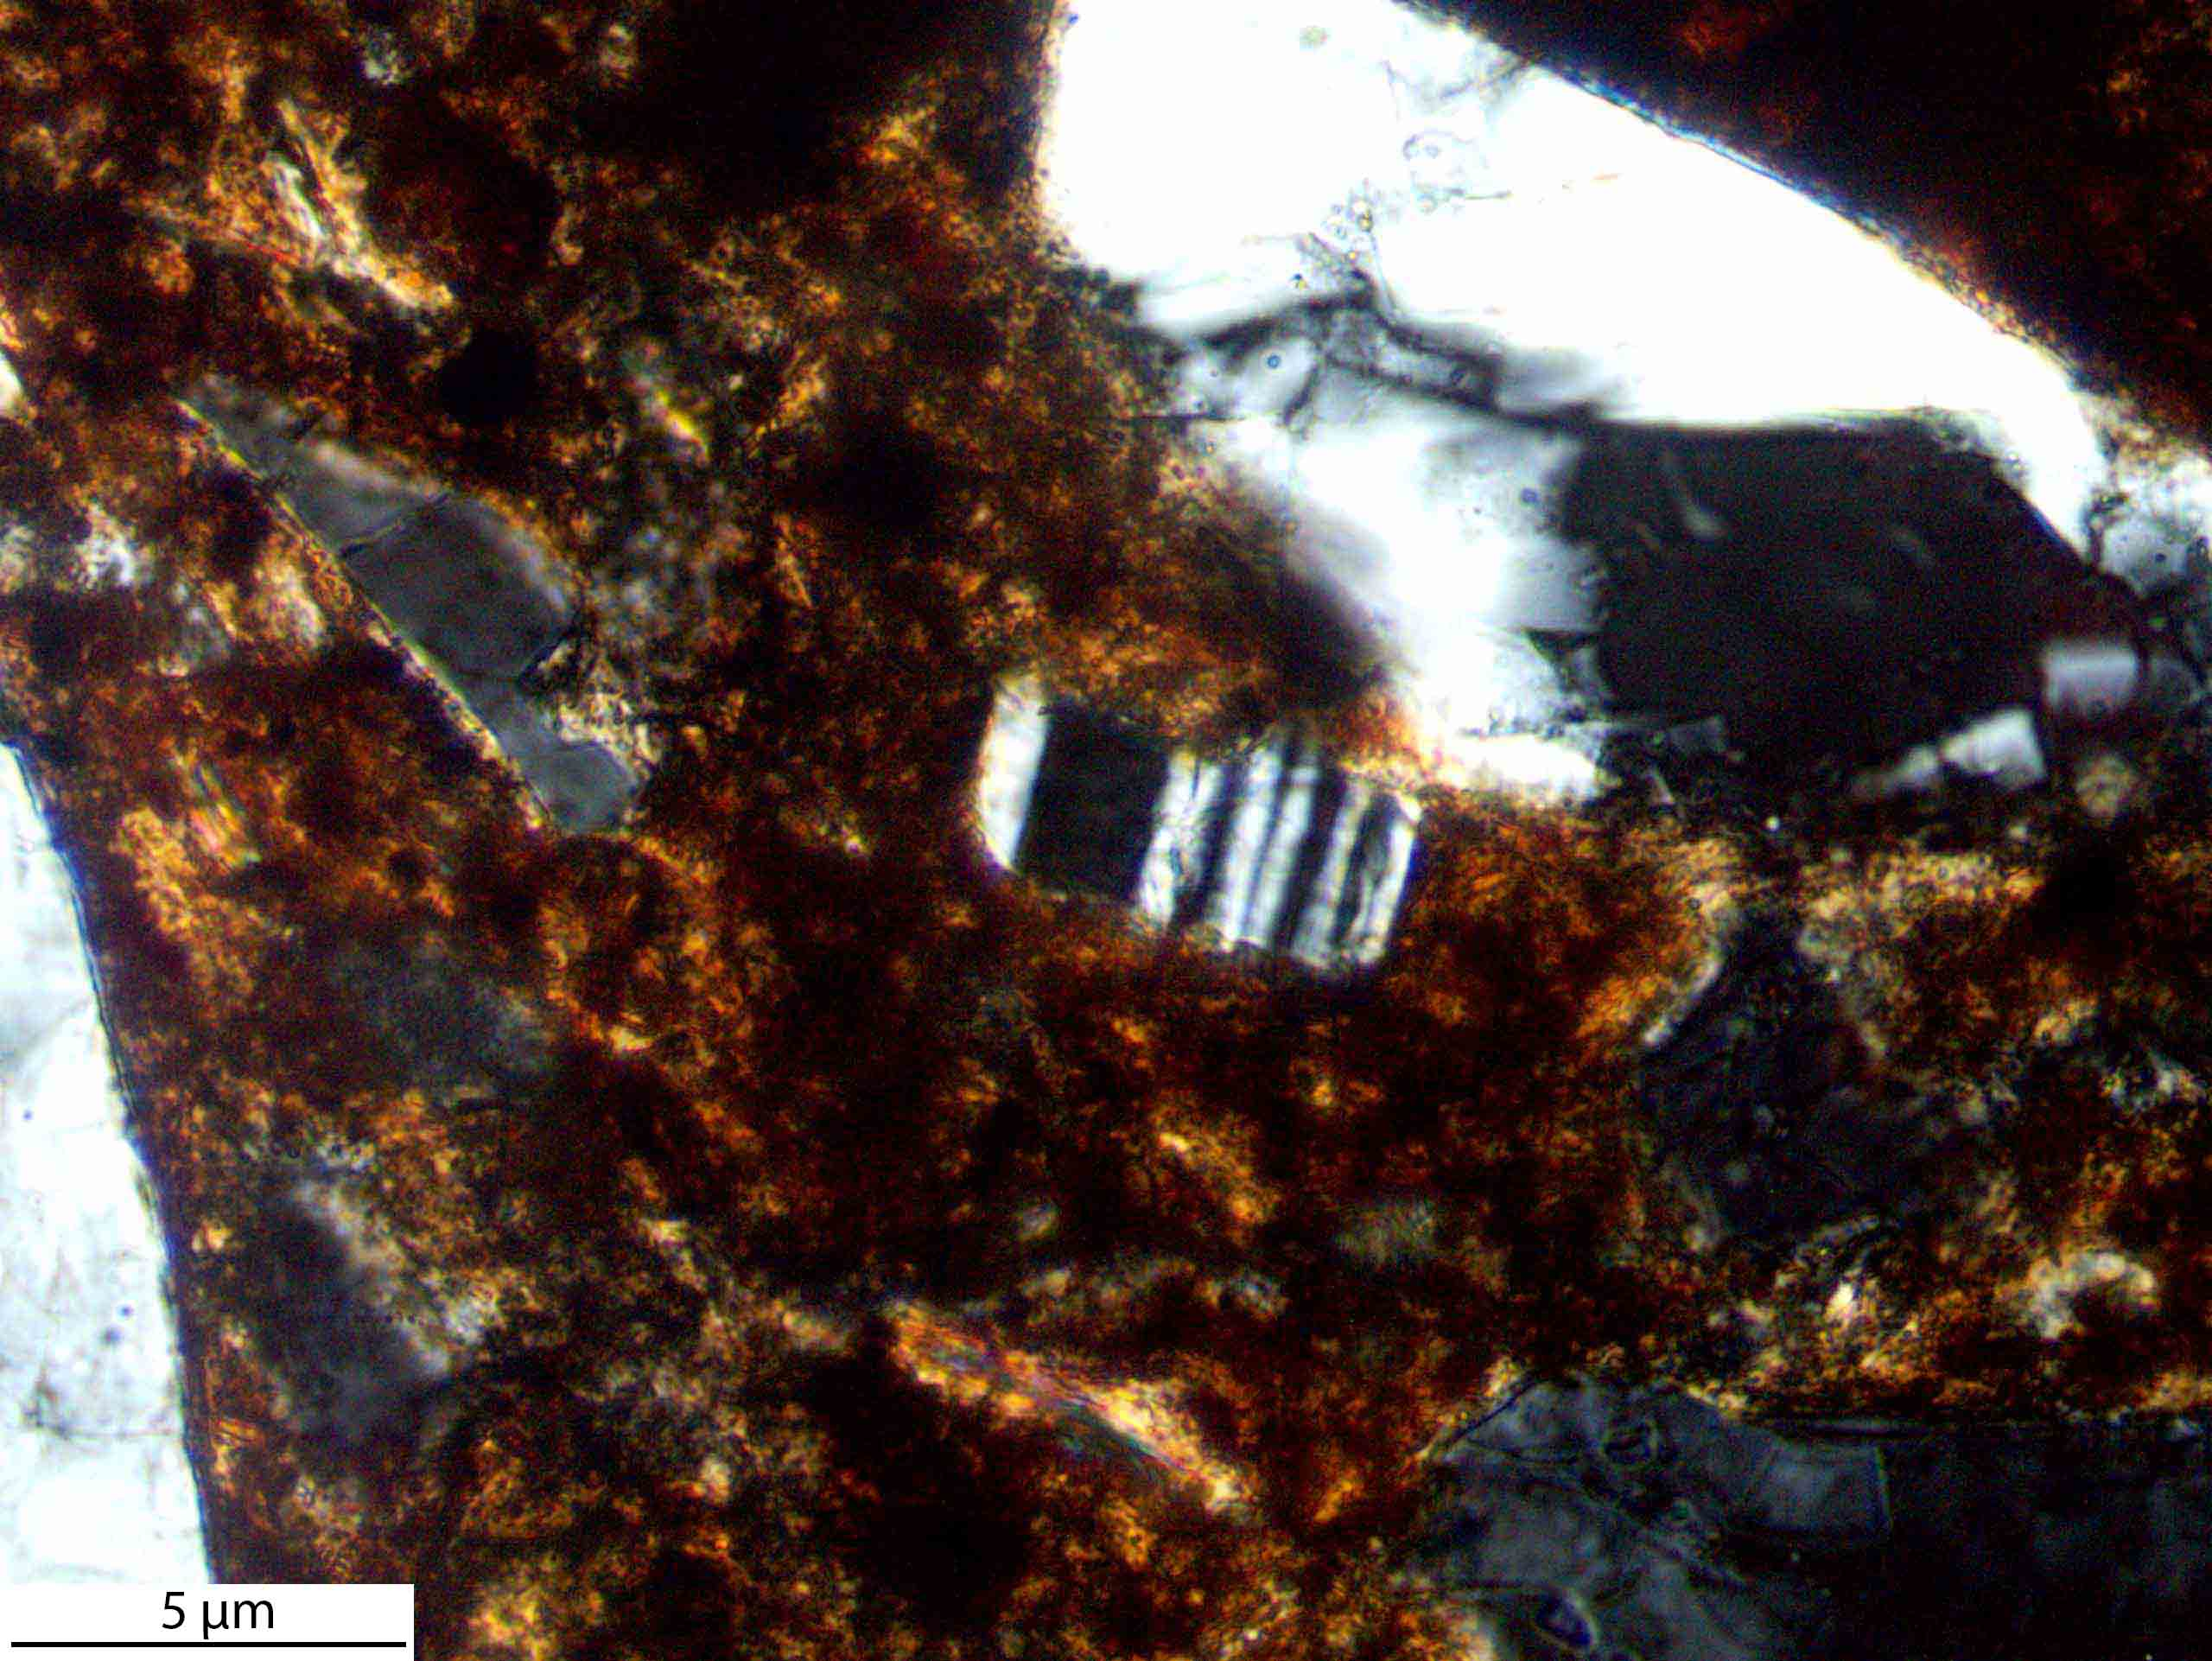
\includegraphics[width=\textwidth]{ThinSections/10-5_40x_XPL.jpg}
		\caption{Plagioclase [XPL]}
	\end{subfigure}
%	\begin{subfigure}[t]{.32\textwidth}
%		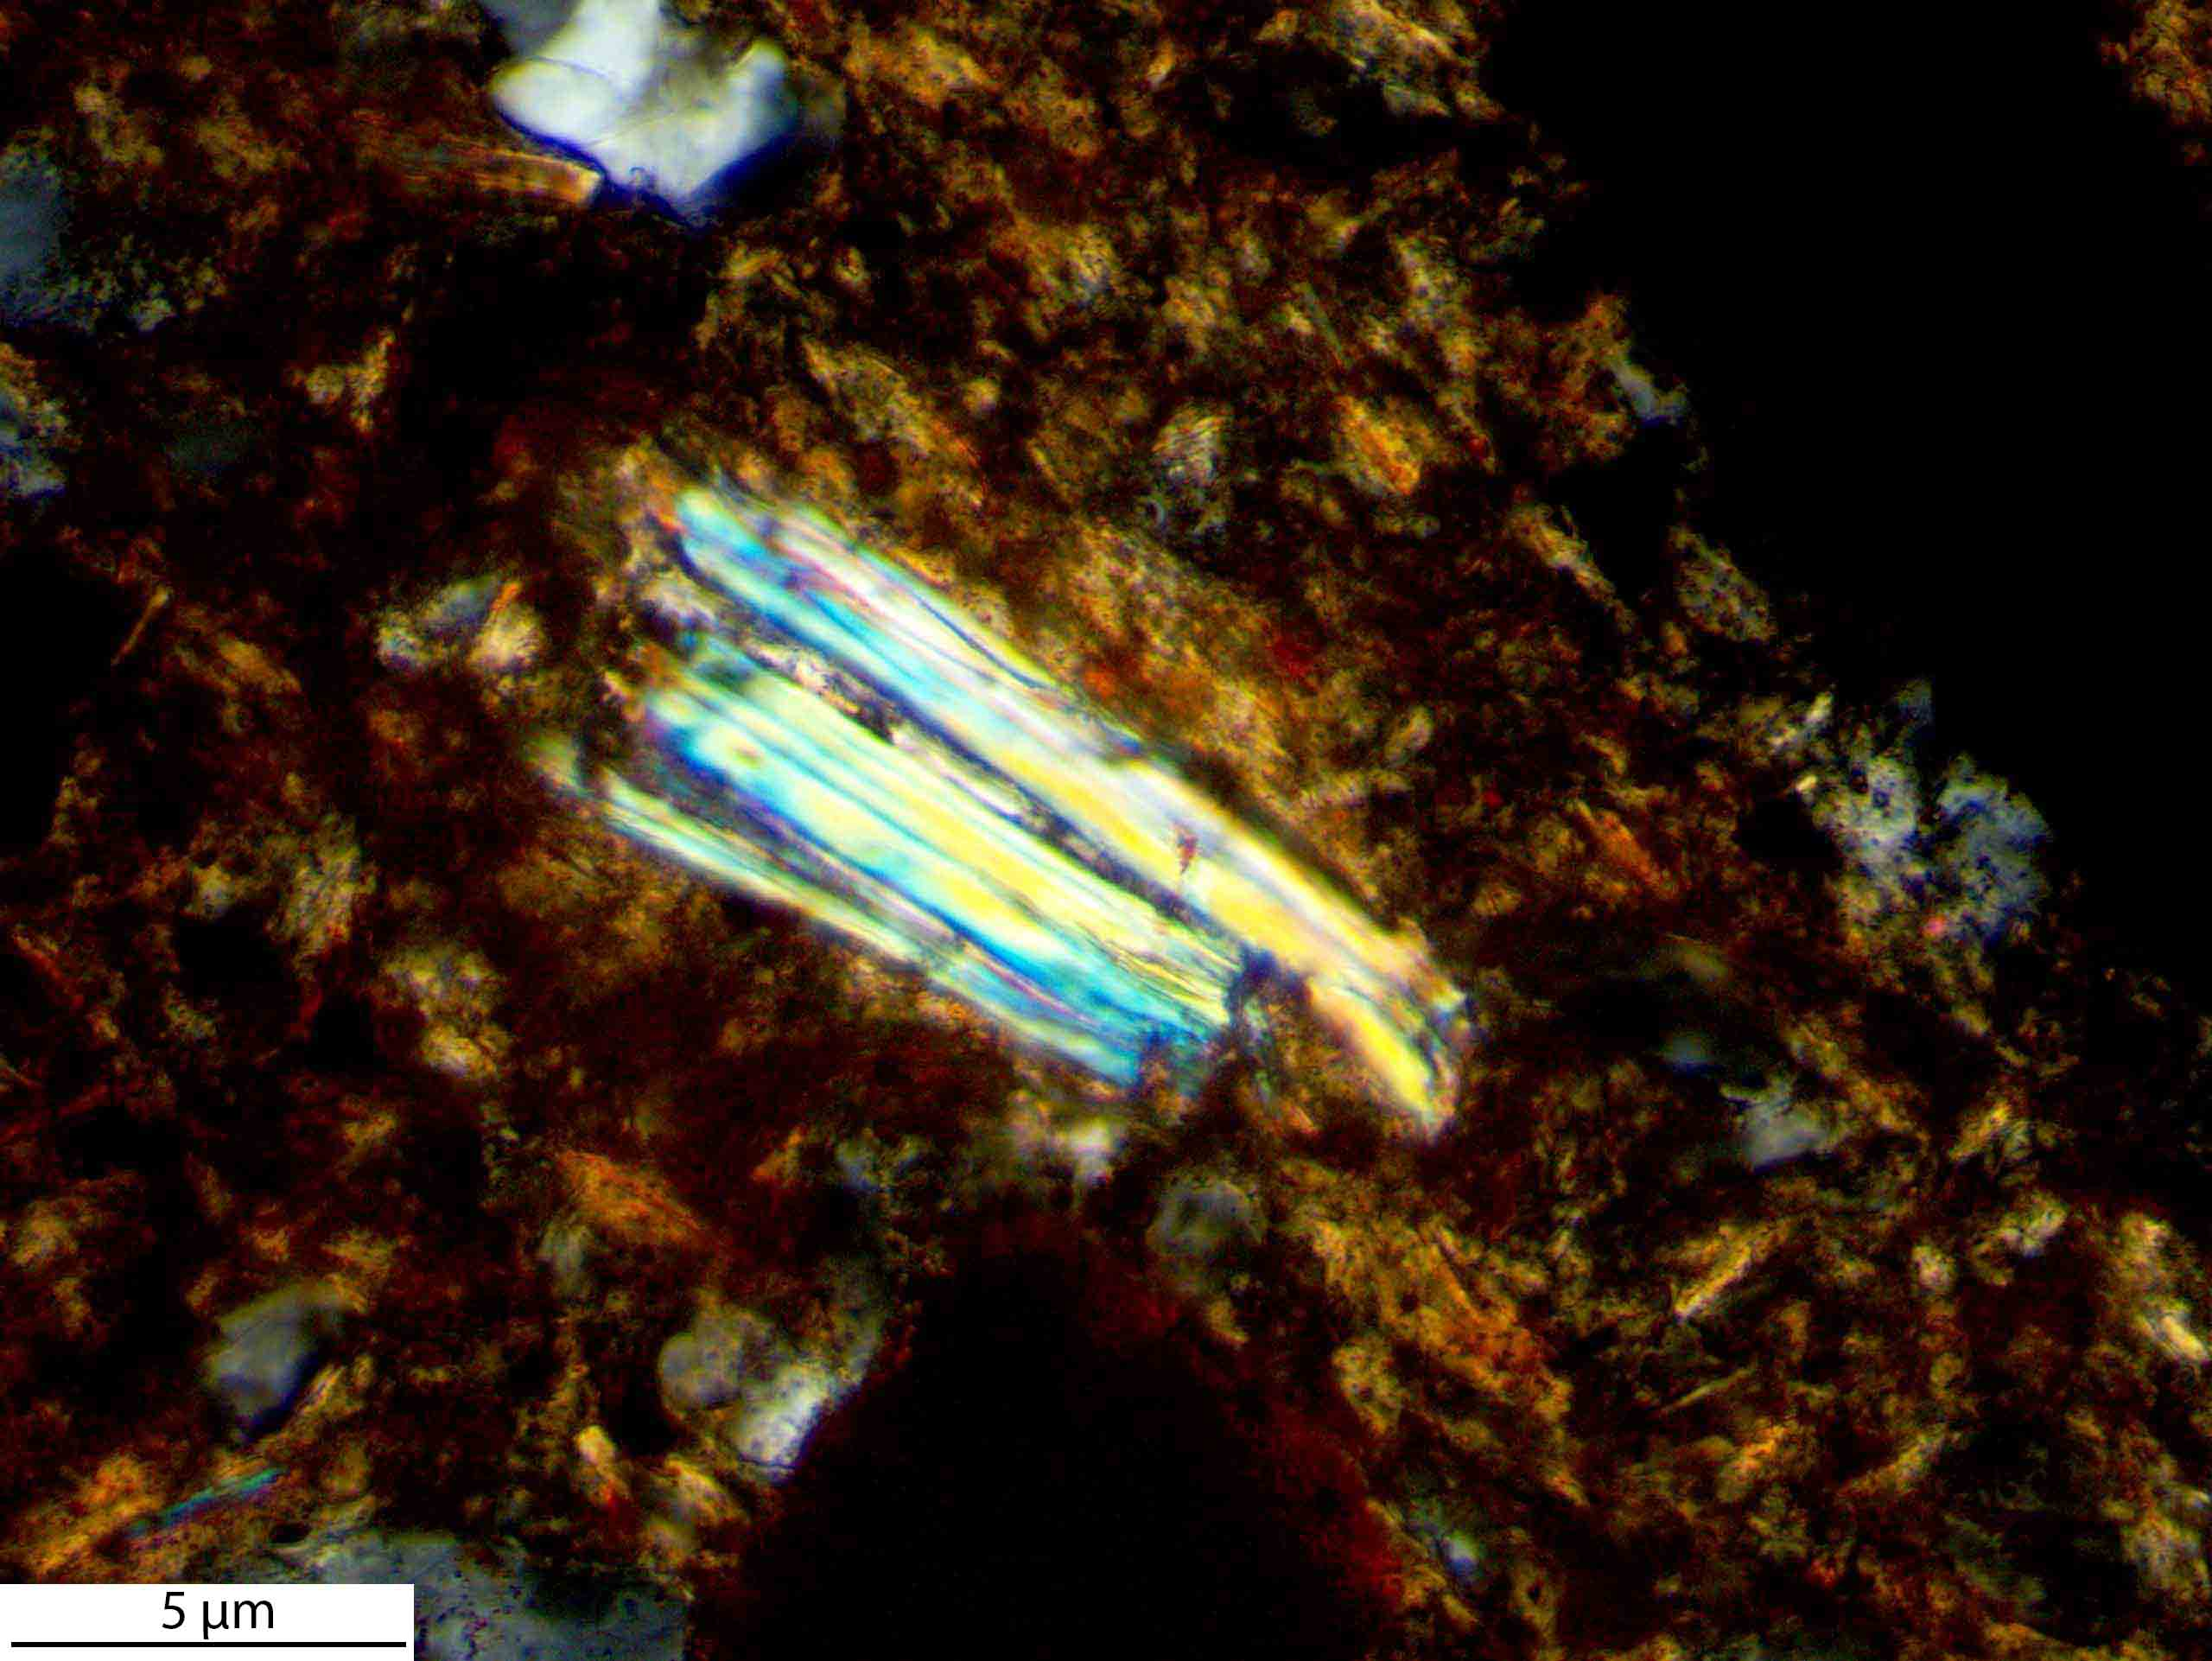
\includegraphics[width=\textwidth]{ThinSections/10-4_40x_XPL.jpg}
%		\caption{Muscovite [XPL]}
%	\end{subfigure}\hspace{.1em}\hfill
%	\begin{subfigure}[t]{.32\textwidth}
%		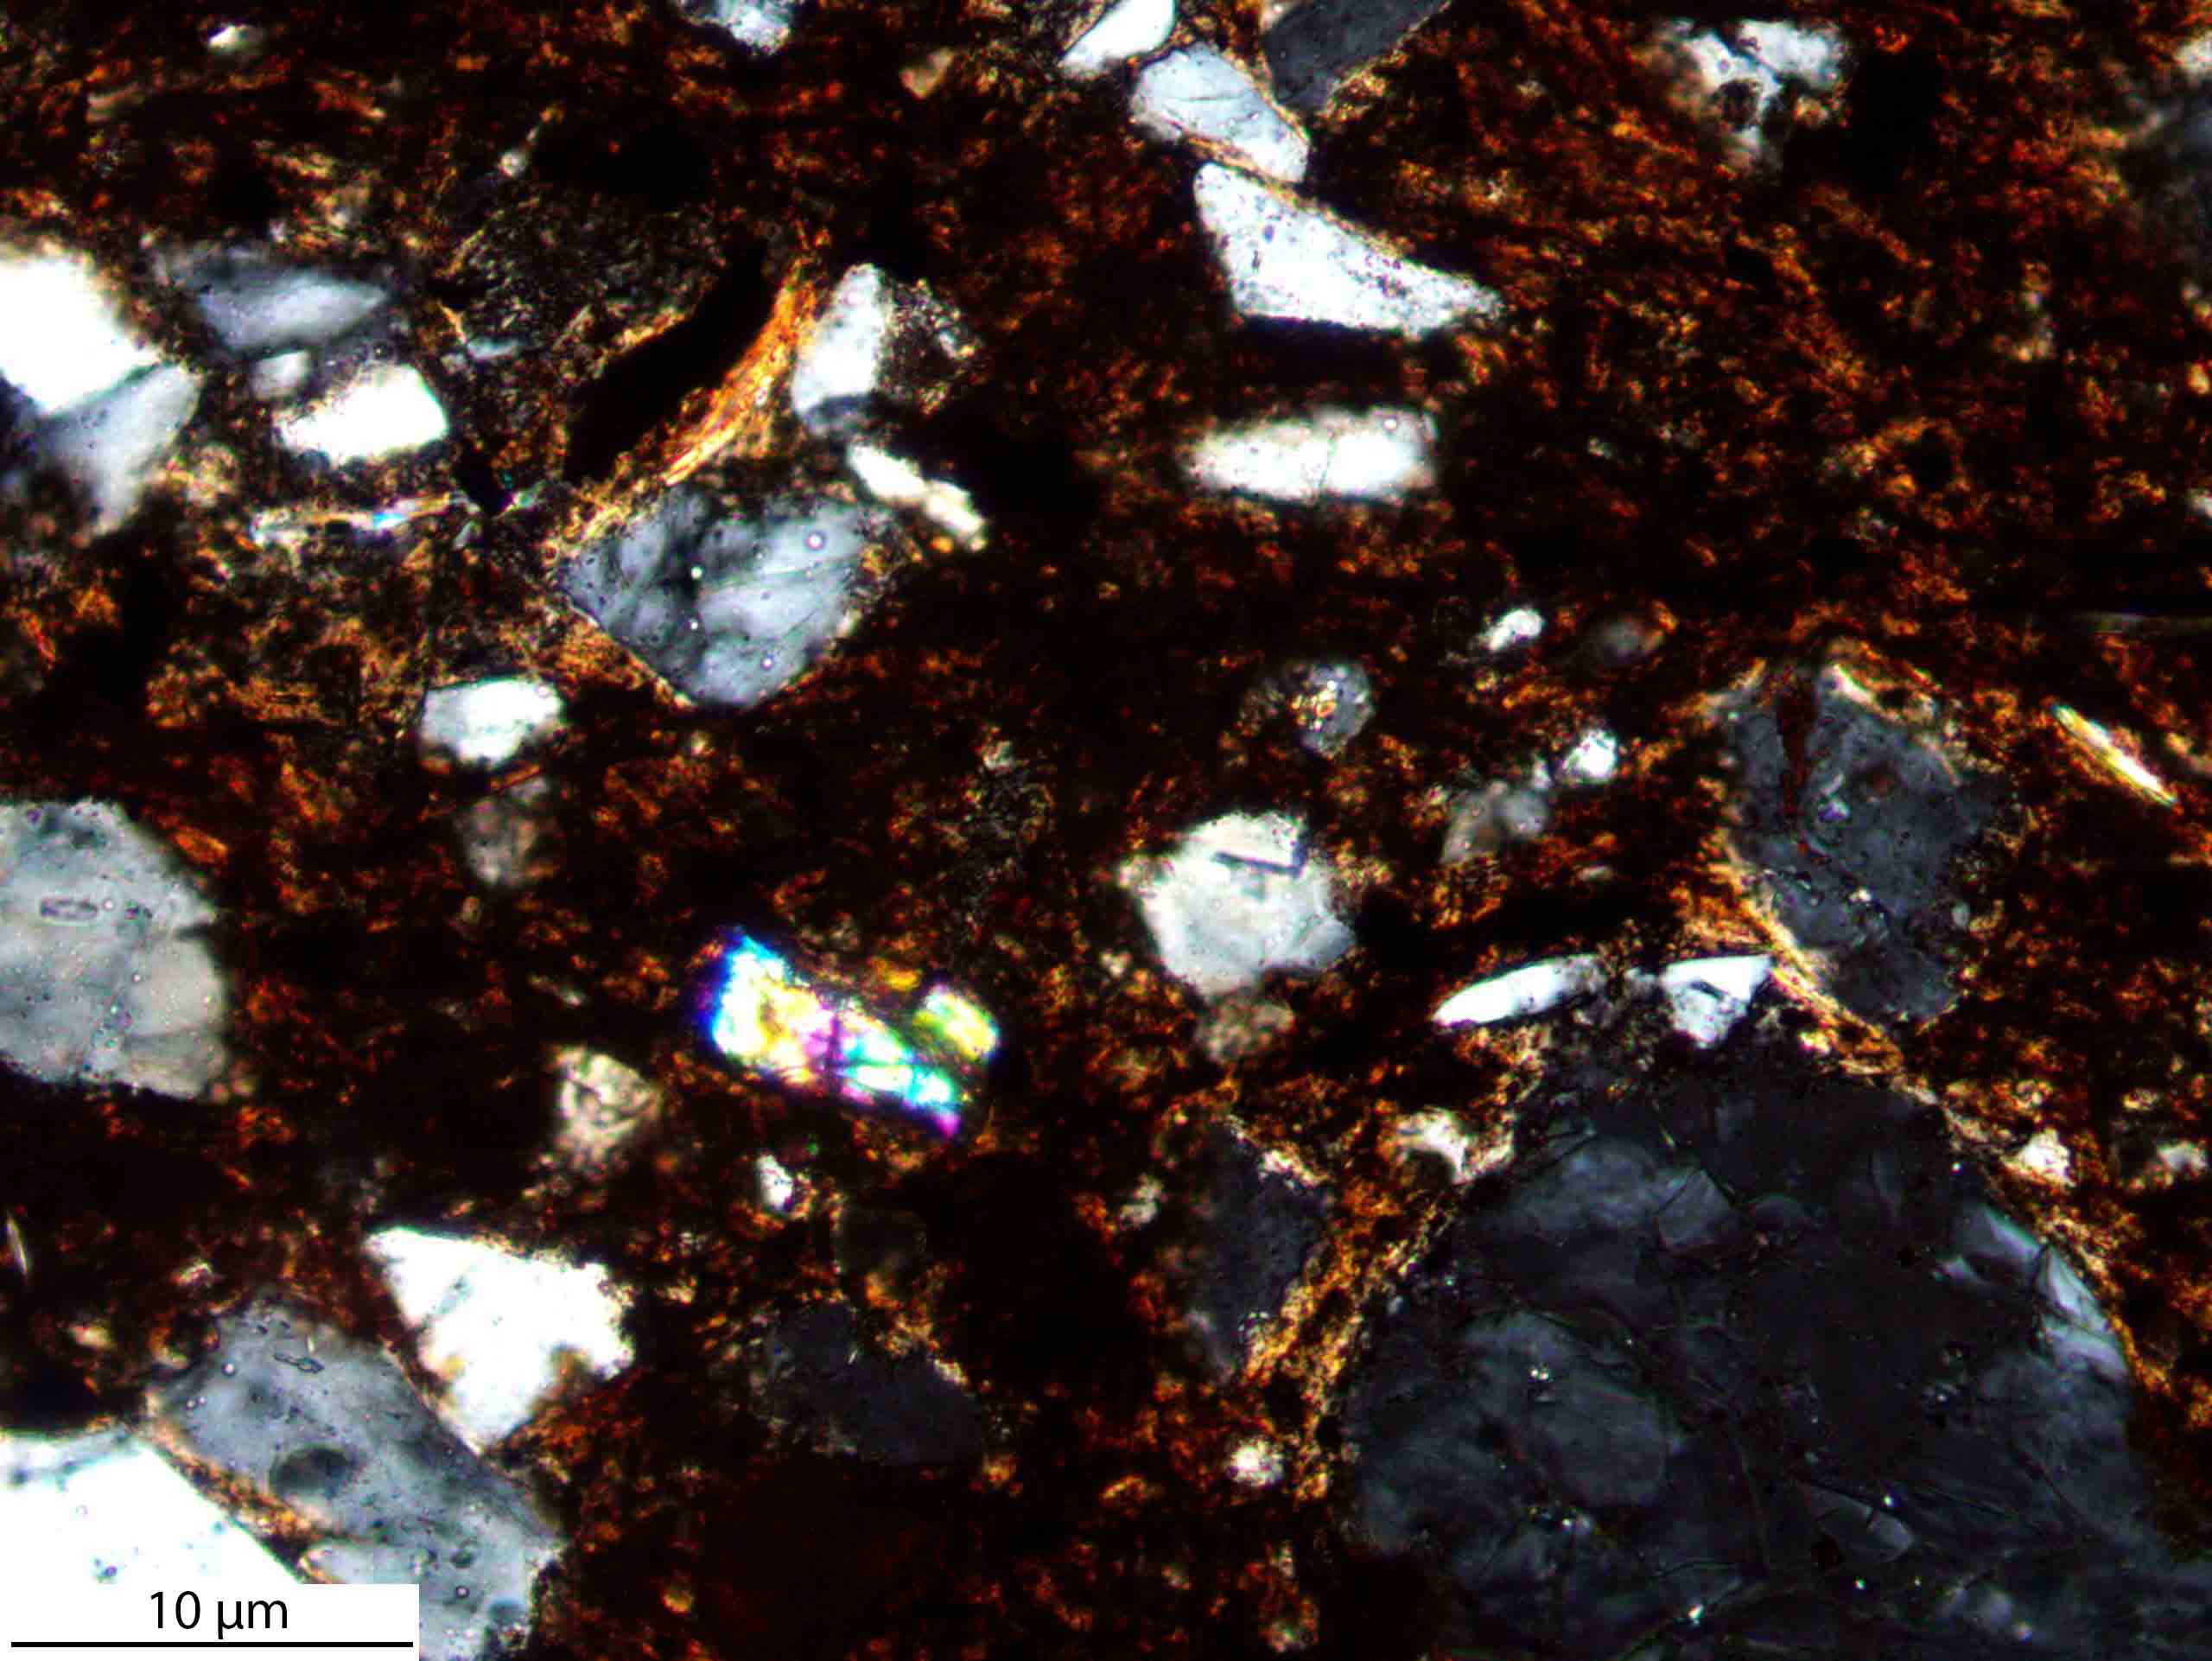
\includegraphics[width=\textwidth]{ThinSections/10-6_20x_XPL.jpg}
%		\caption{Zircon [XPL]}
%	\end{subfigure}
	\caption{}
	\label{fig:10_pik}
\end{figure}

\newpage\subsection{PIK~87/1-7:12 \citep[pik\#4; Fig.~\ref{fig:pik.pottery}.3; Pikunda-Munda style;][427 Pl.~46.21]{Seidensticker.2021e}}

\begin{multicols}{2}
\noindent The samples fine fraction (light yellowish to dark brown [PPL]) is heterogeneous and non-calcareous with stipple-speckled b-fabric. Voids are rare or very narrow, without any discernible orientation. The main component of the coarse fraction are sponge spicules. These are mostly cut transverse and lesser longitudinal in relation to the plane of the section. Also dominant part of the coarse fraction is fine quartz in an unimodal grain-size distribution. Occasionally, the larger fraction of quartz particles consists of runiquartz or rock fragments (sandstone) (e). To a lesser degree present are biotite and muscovite as well as plagioclas (f), kyanite (c--d) and zircone. The c/f-related distribution pattern is single-spaced porphyric.
\end{multicols}

% dark patches due to perperation of the slide!
% -> check section @high magnification > dark stuff sharp "higher"
% rutile grain > dark brown PPL & gold XPL & high relief
% FM: tourmaline; pinkish zone

%\vfill
\begin{figure}[H]
	\centering
	\begin{subfigure}[t]{.49\textwidth}
		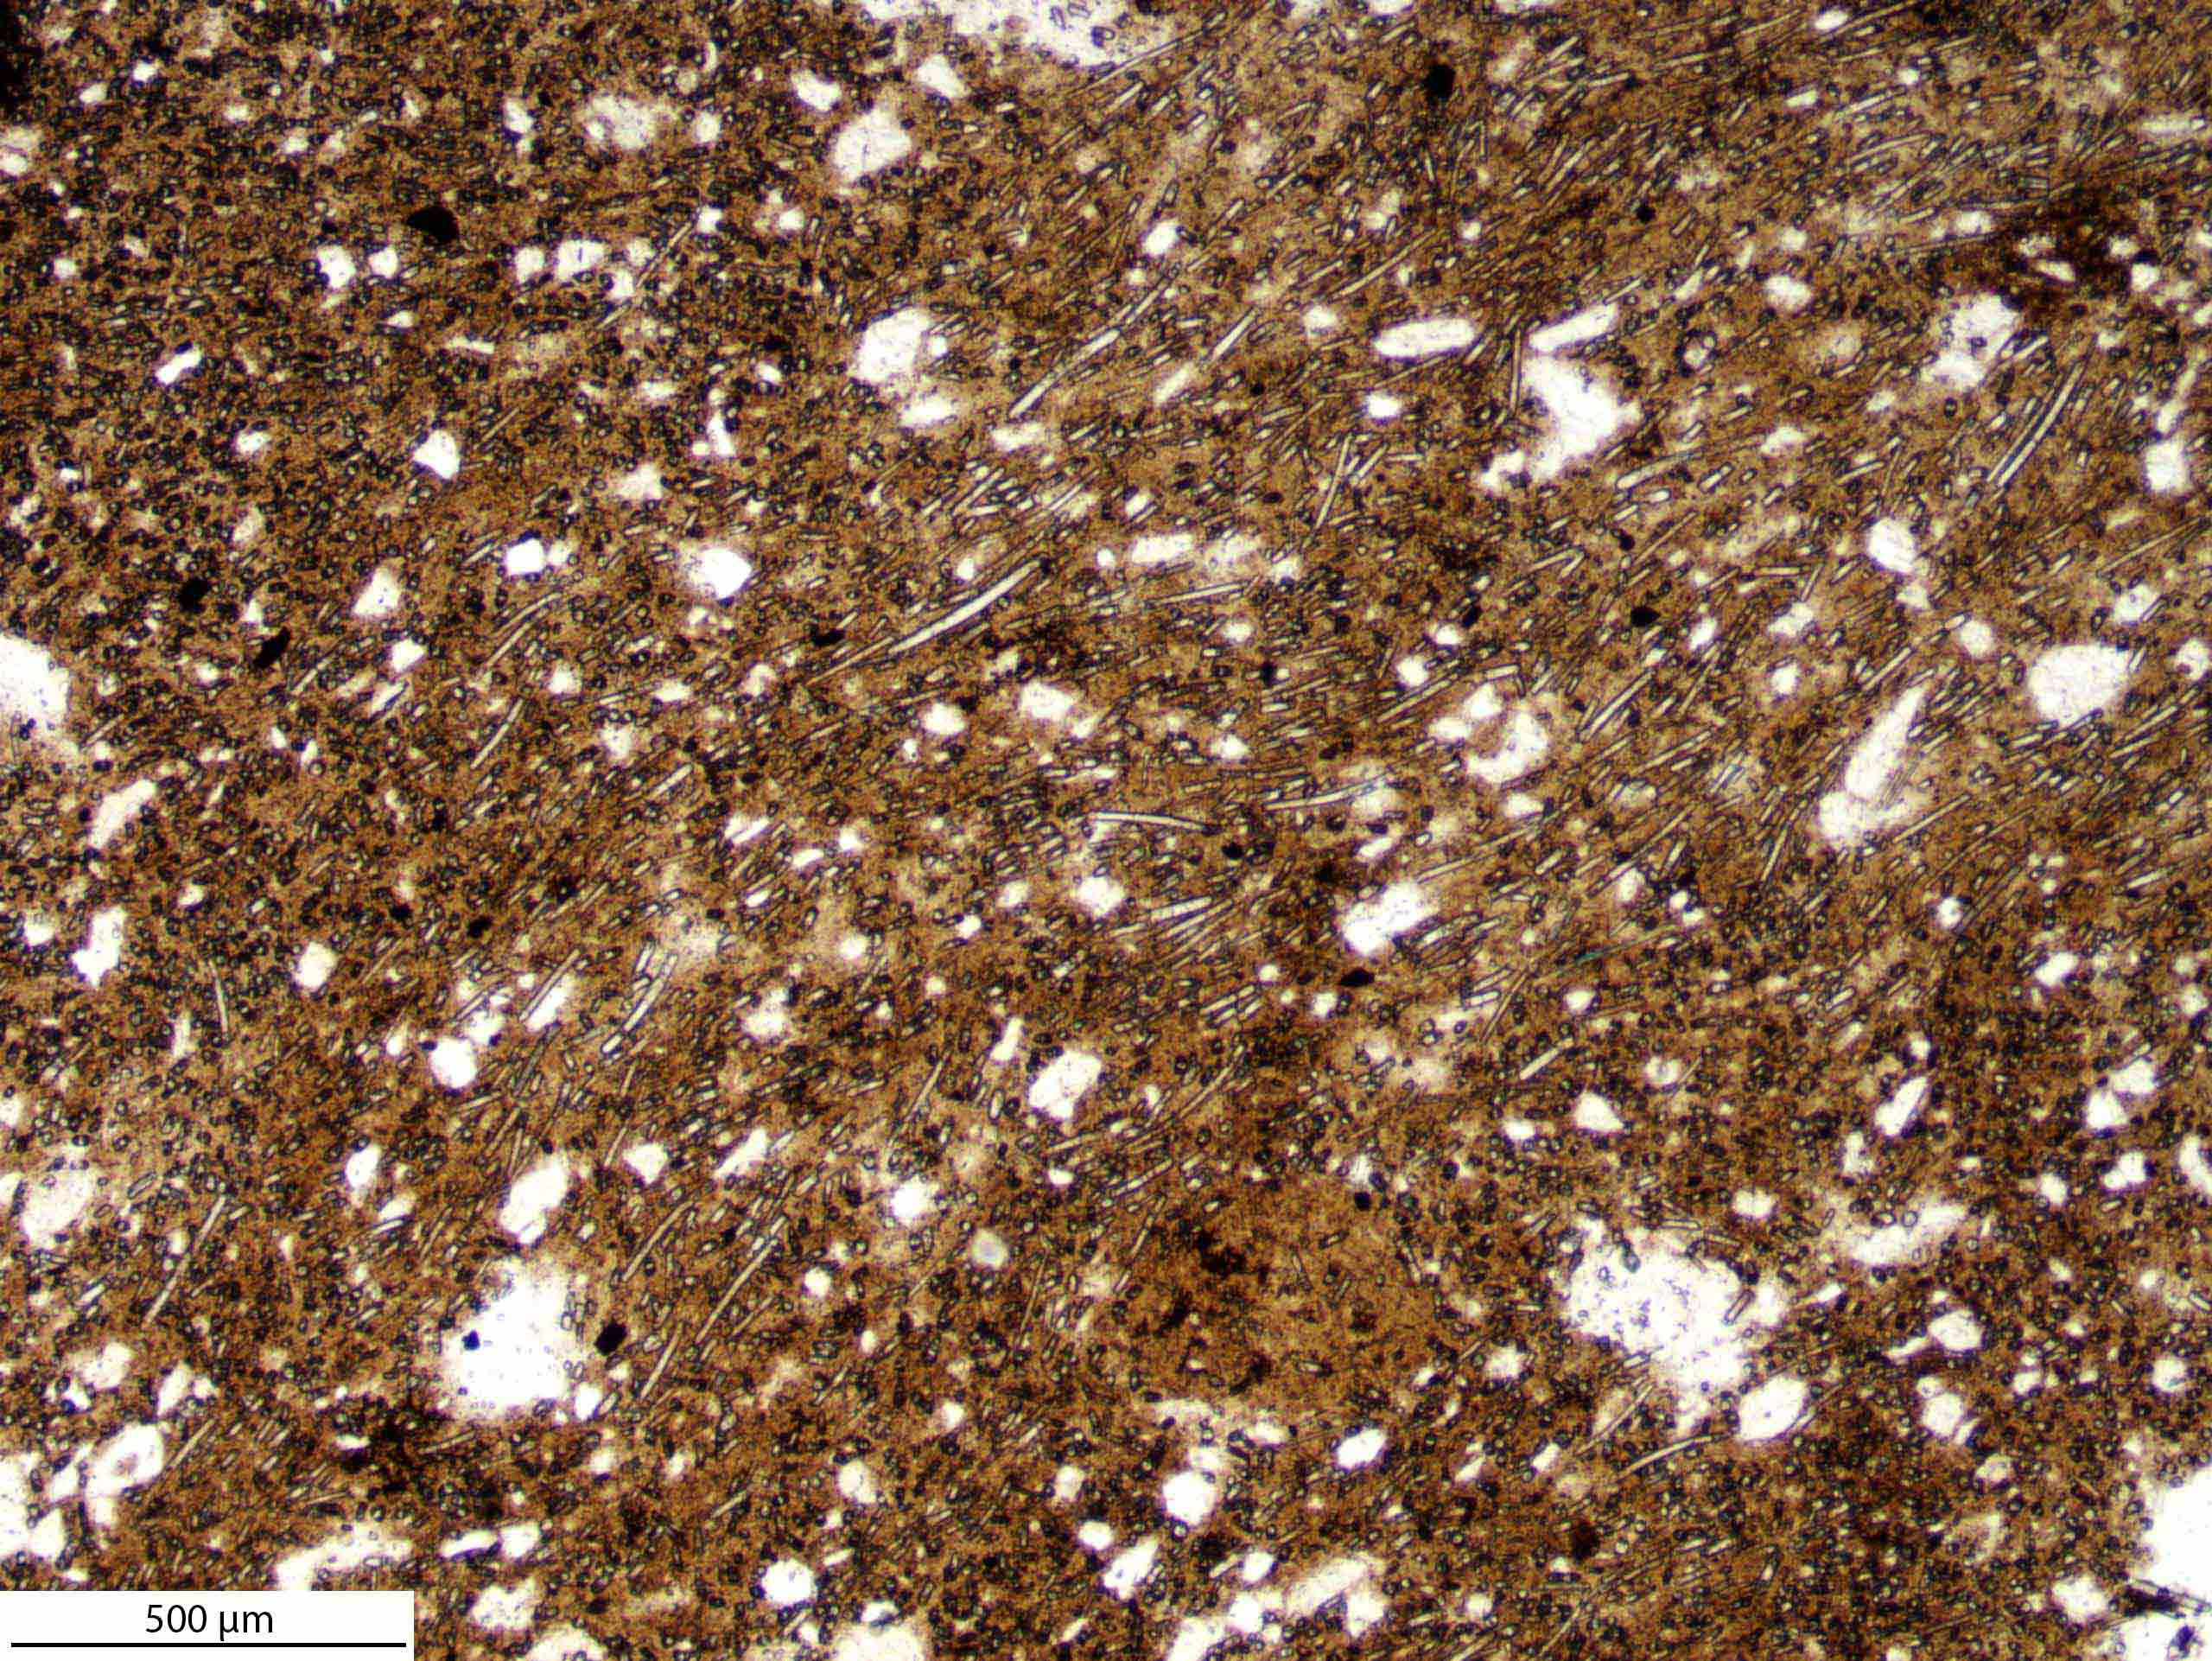
\includegraphics[width=\textwidth]{ThinSections/4-1_4x_PPL.jpg}
		\caption{[PPL]}
	\end{subfigure}\hspace{.5em}\hfill
	\begin{subfigure}[t]{.49\textwidth}
		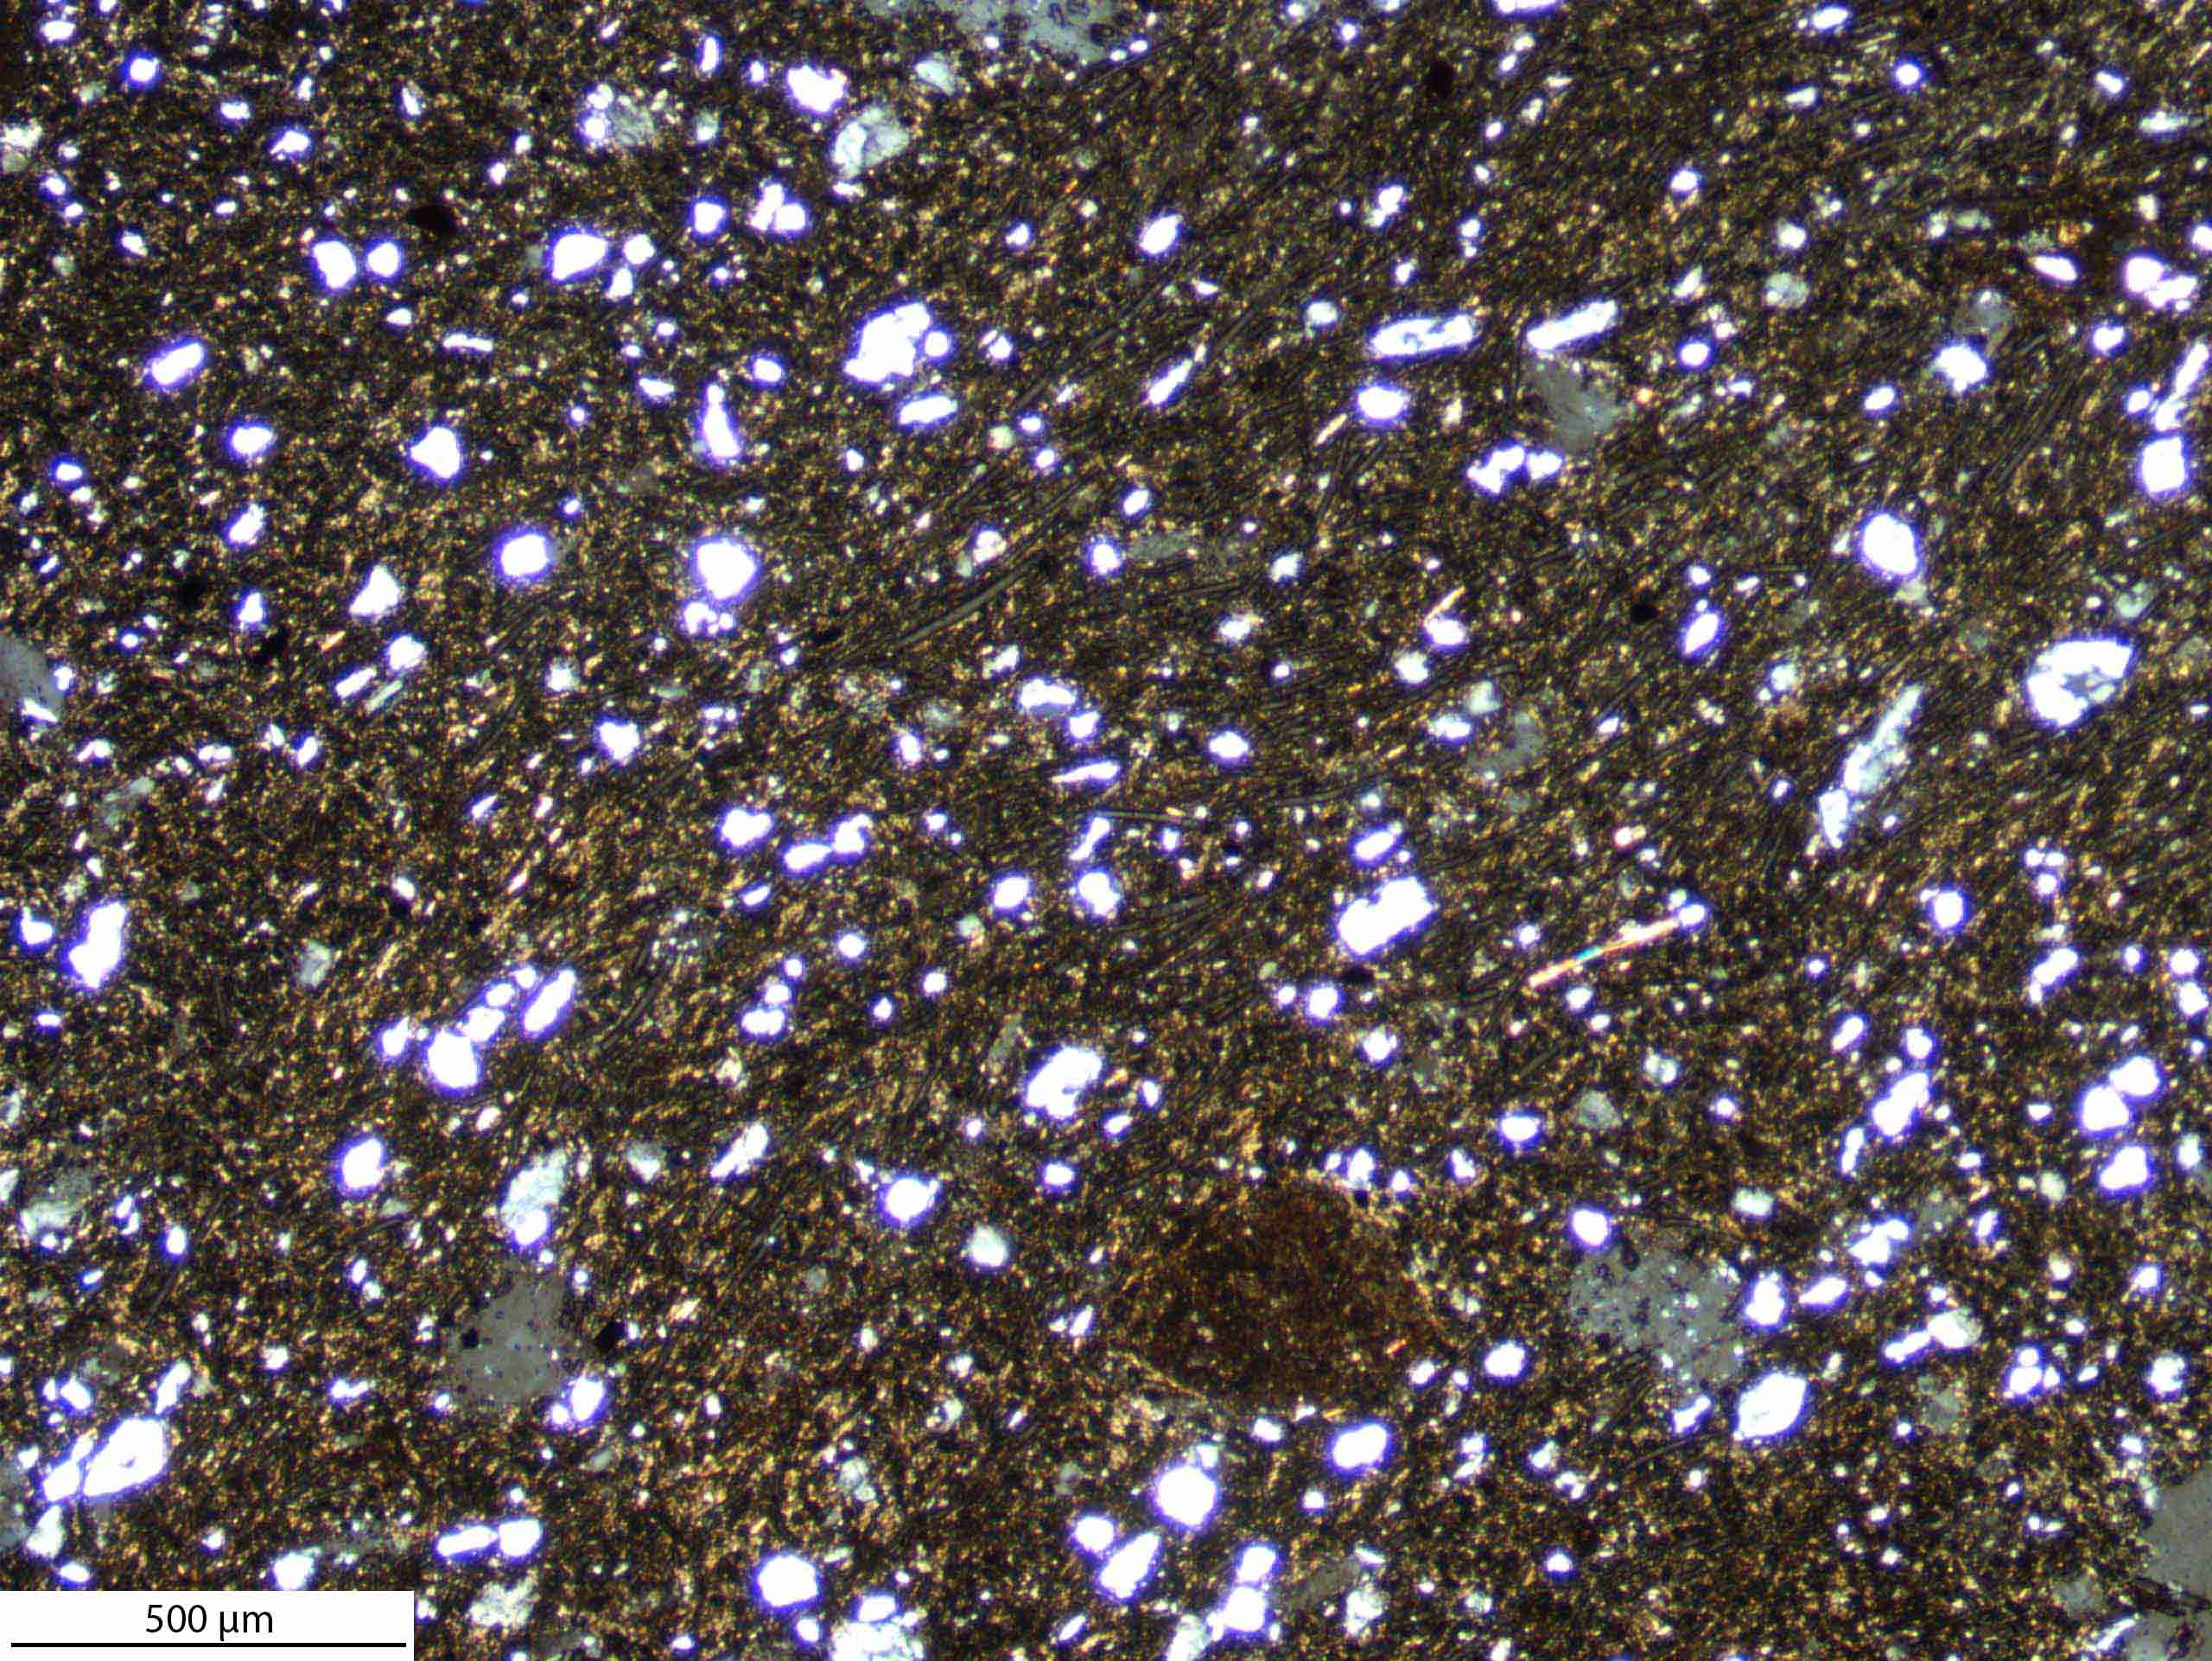
\includegraphics[width=\textwidth]{ThinSections/4-1_4x_XPL.jpg}
		\caption{[XPL]}
	\end{subfigure}
%	\begin{subfigure}[t]{.24\textwidth}
%		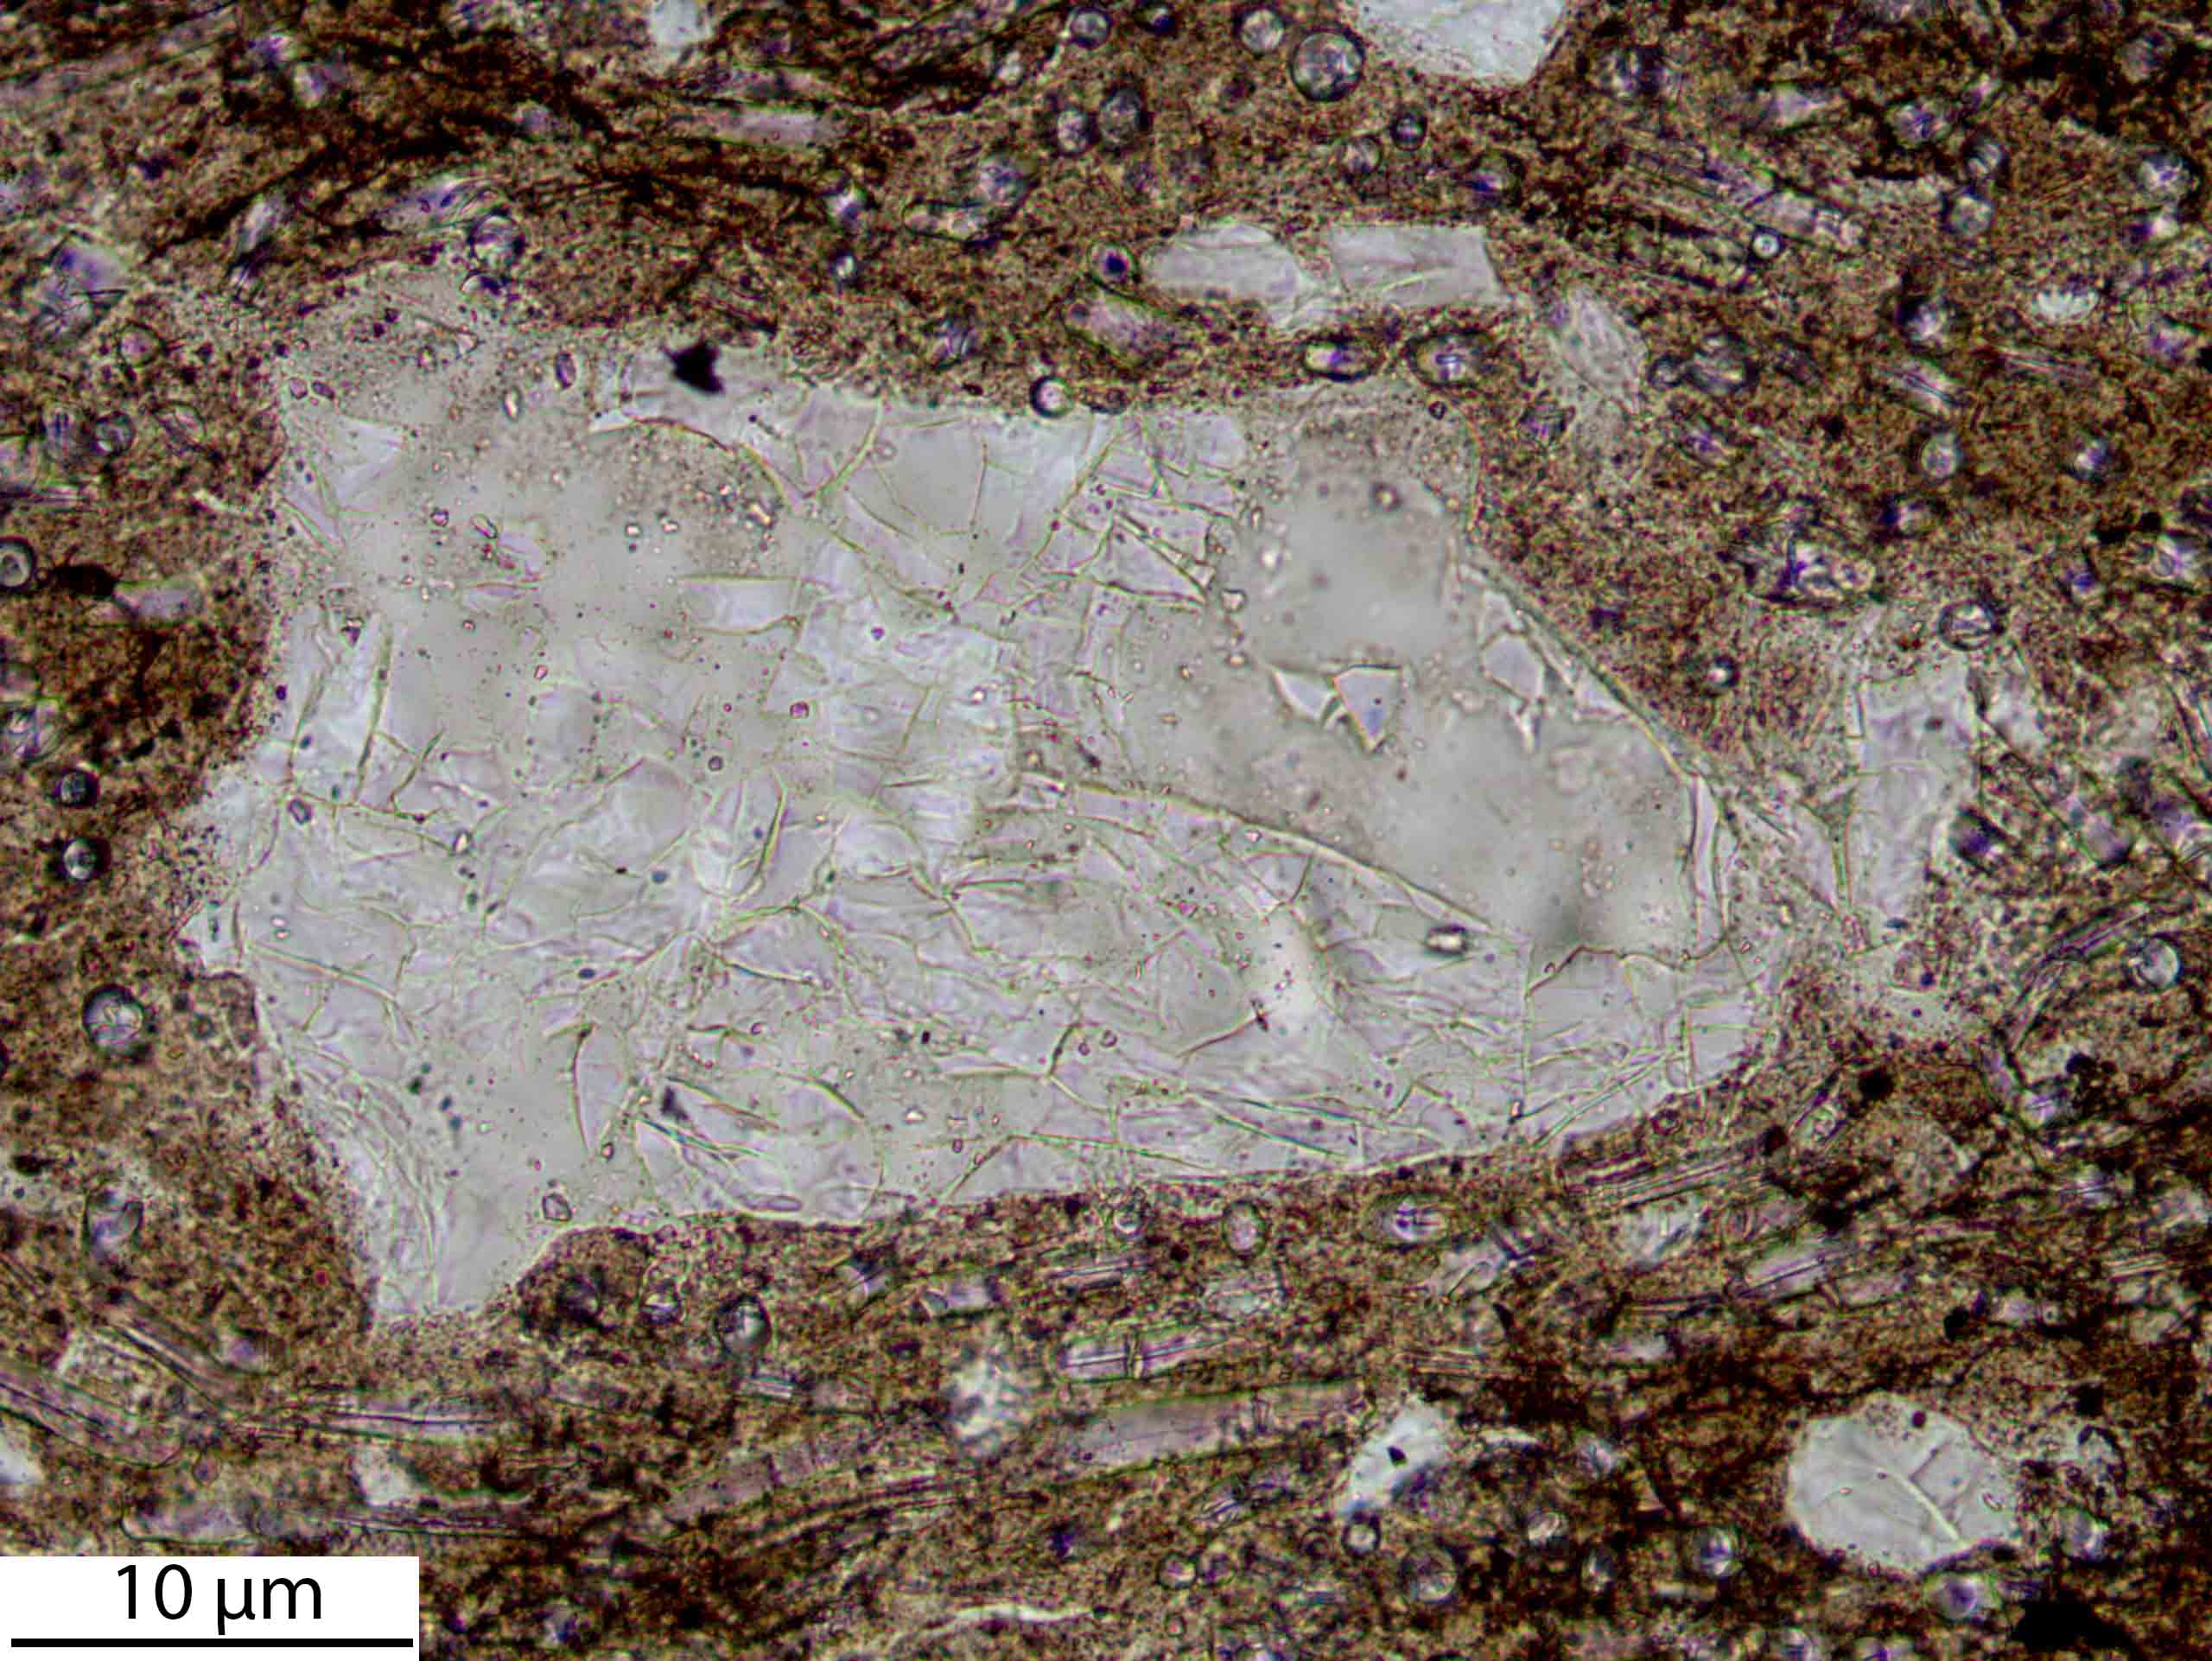
\includegraphics[width=\textwidth]{ThinSections/4-4_20x_PPL.jpg}
%		\caption{Rock fragment [PPL]}
%	\end{subfigure}\hspace{.1em}\hfill
	\begin{subfigure}[t]{.24\textwidth}
		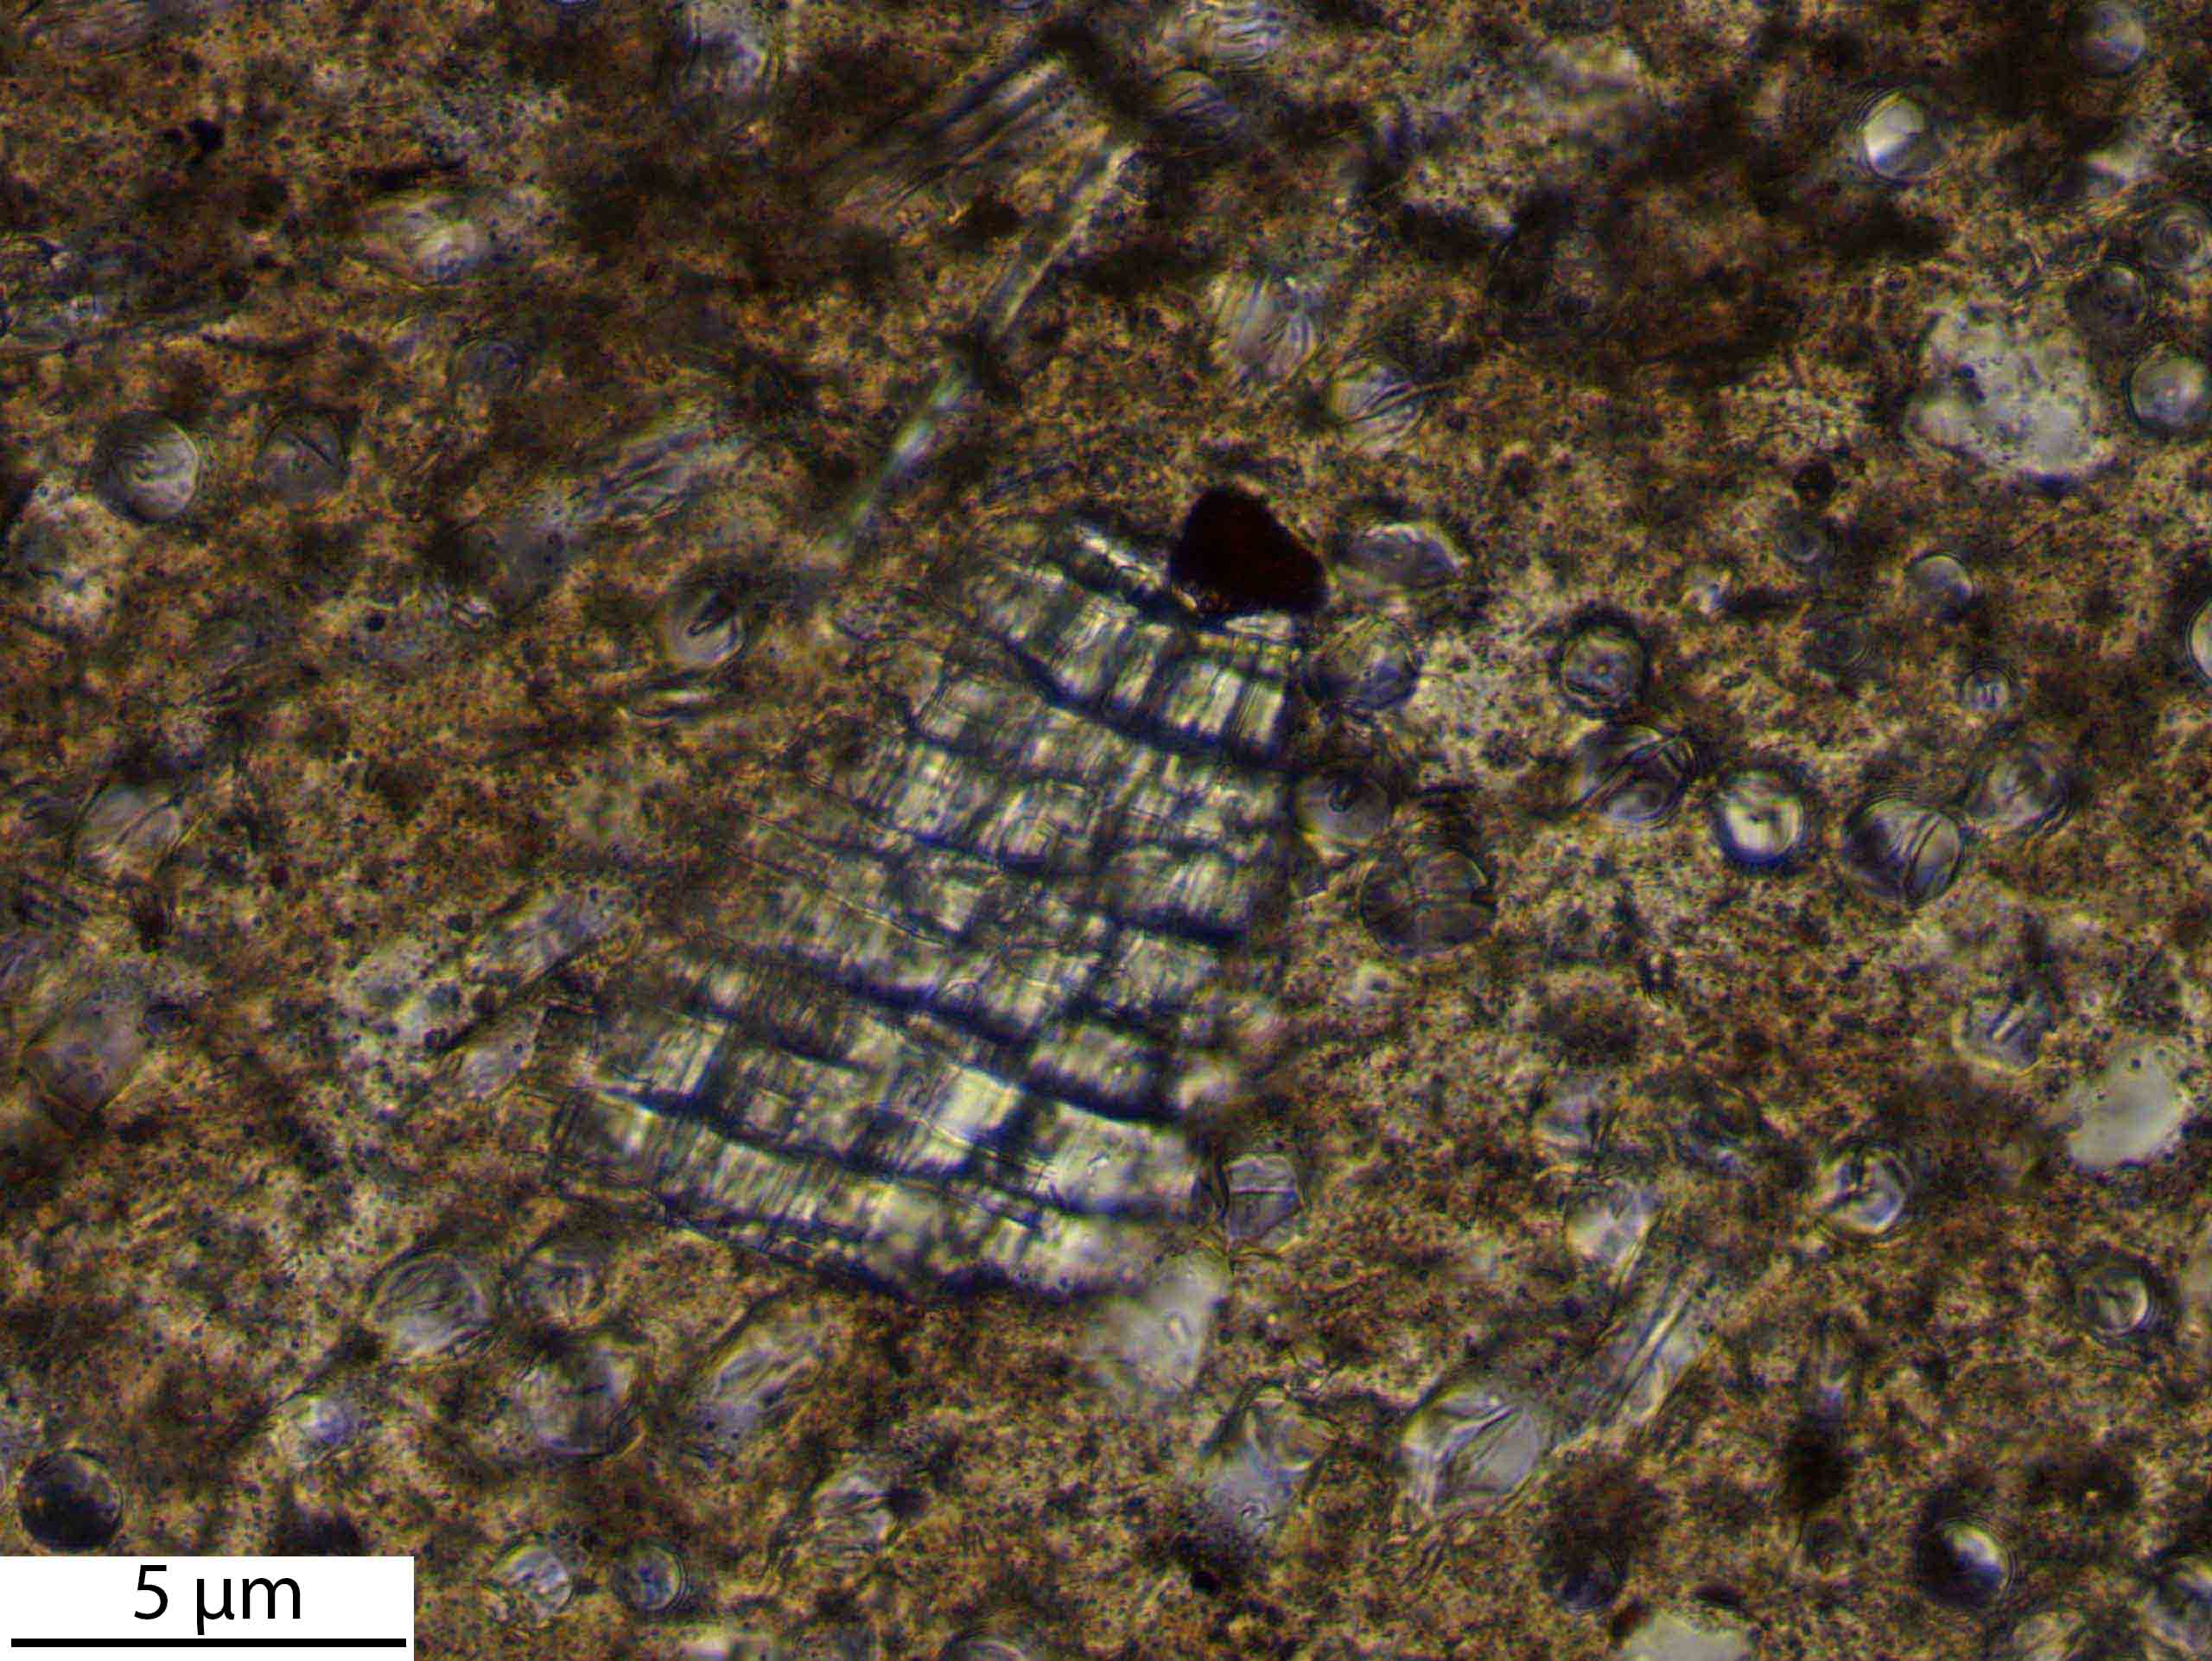
\includegraphics[width=\textwidth]{ThinSections/4-2_40x_PPL.jpg}
		\caption{Kyanite \& muscovite [PPL]}
	\end{subfigure}\hspace{.1em}\hfill
	\begin{subfigure}[t]{.24\textwidth}
		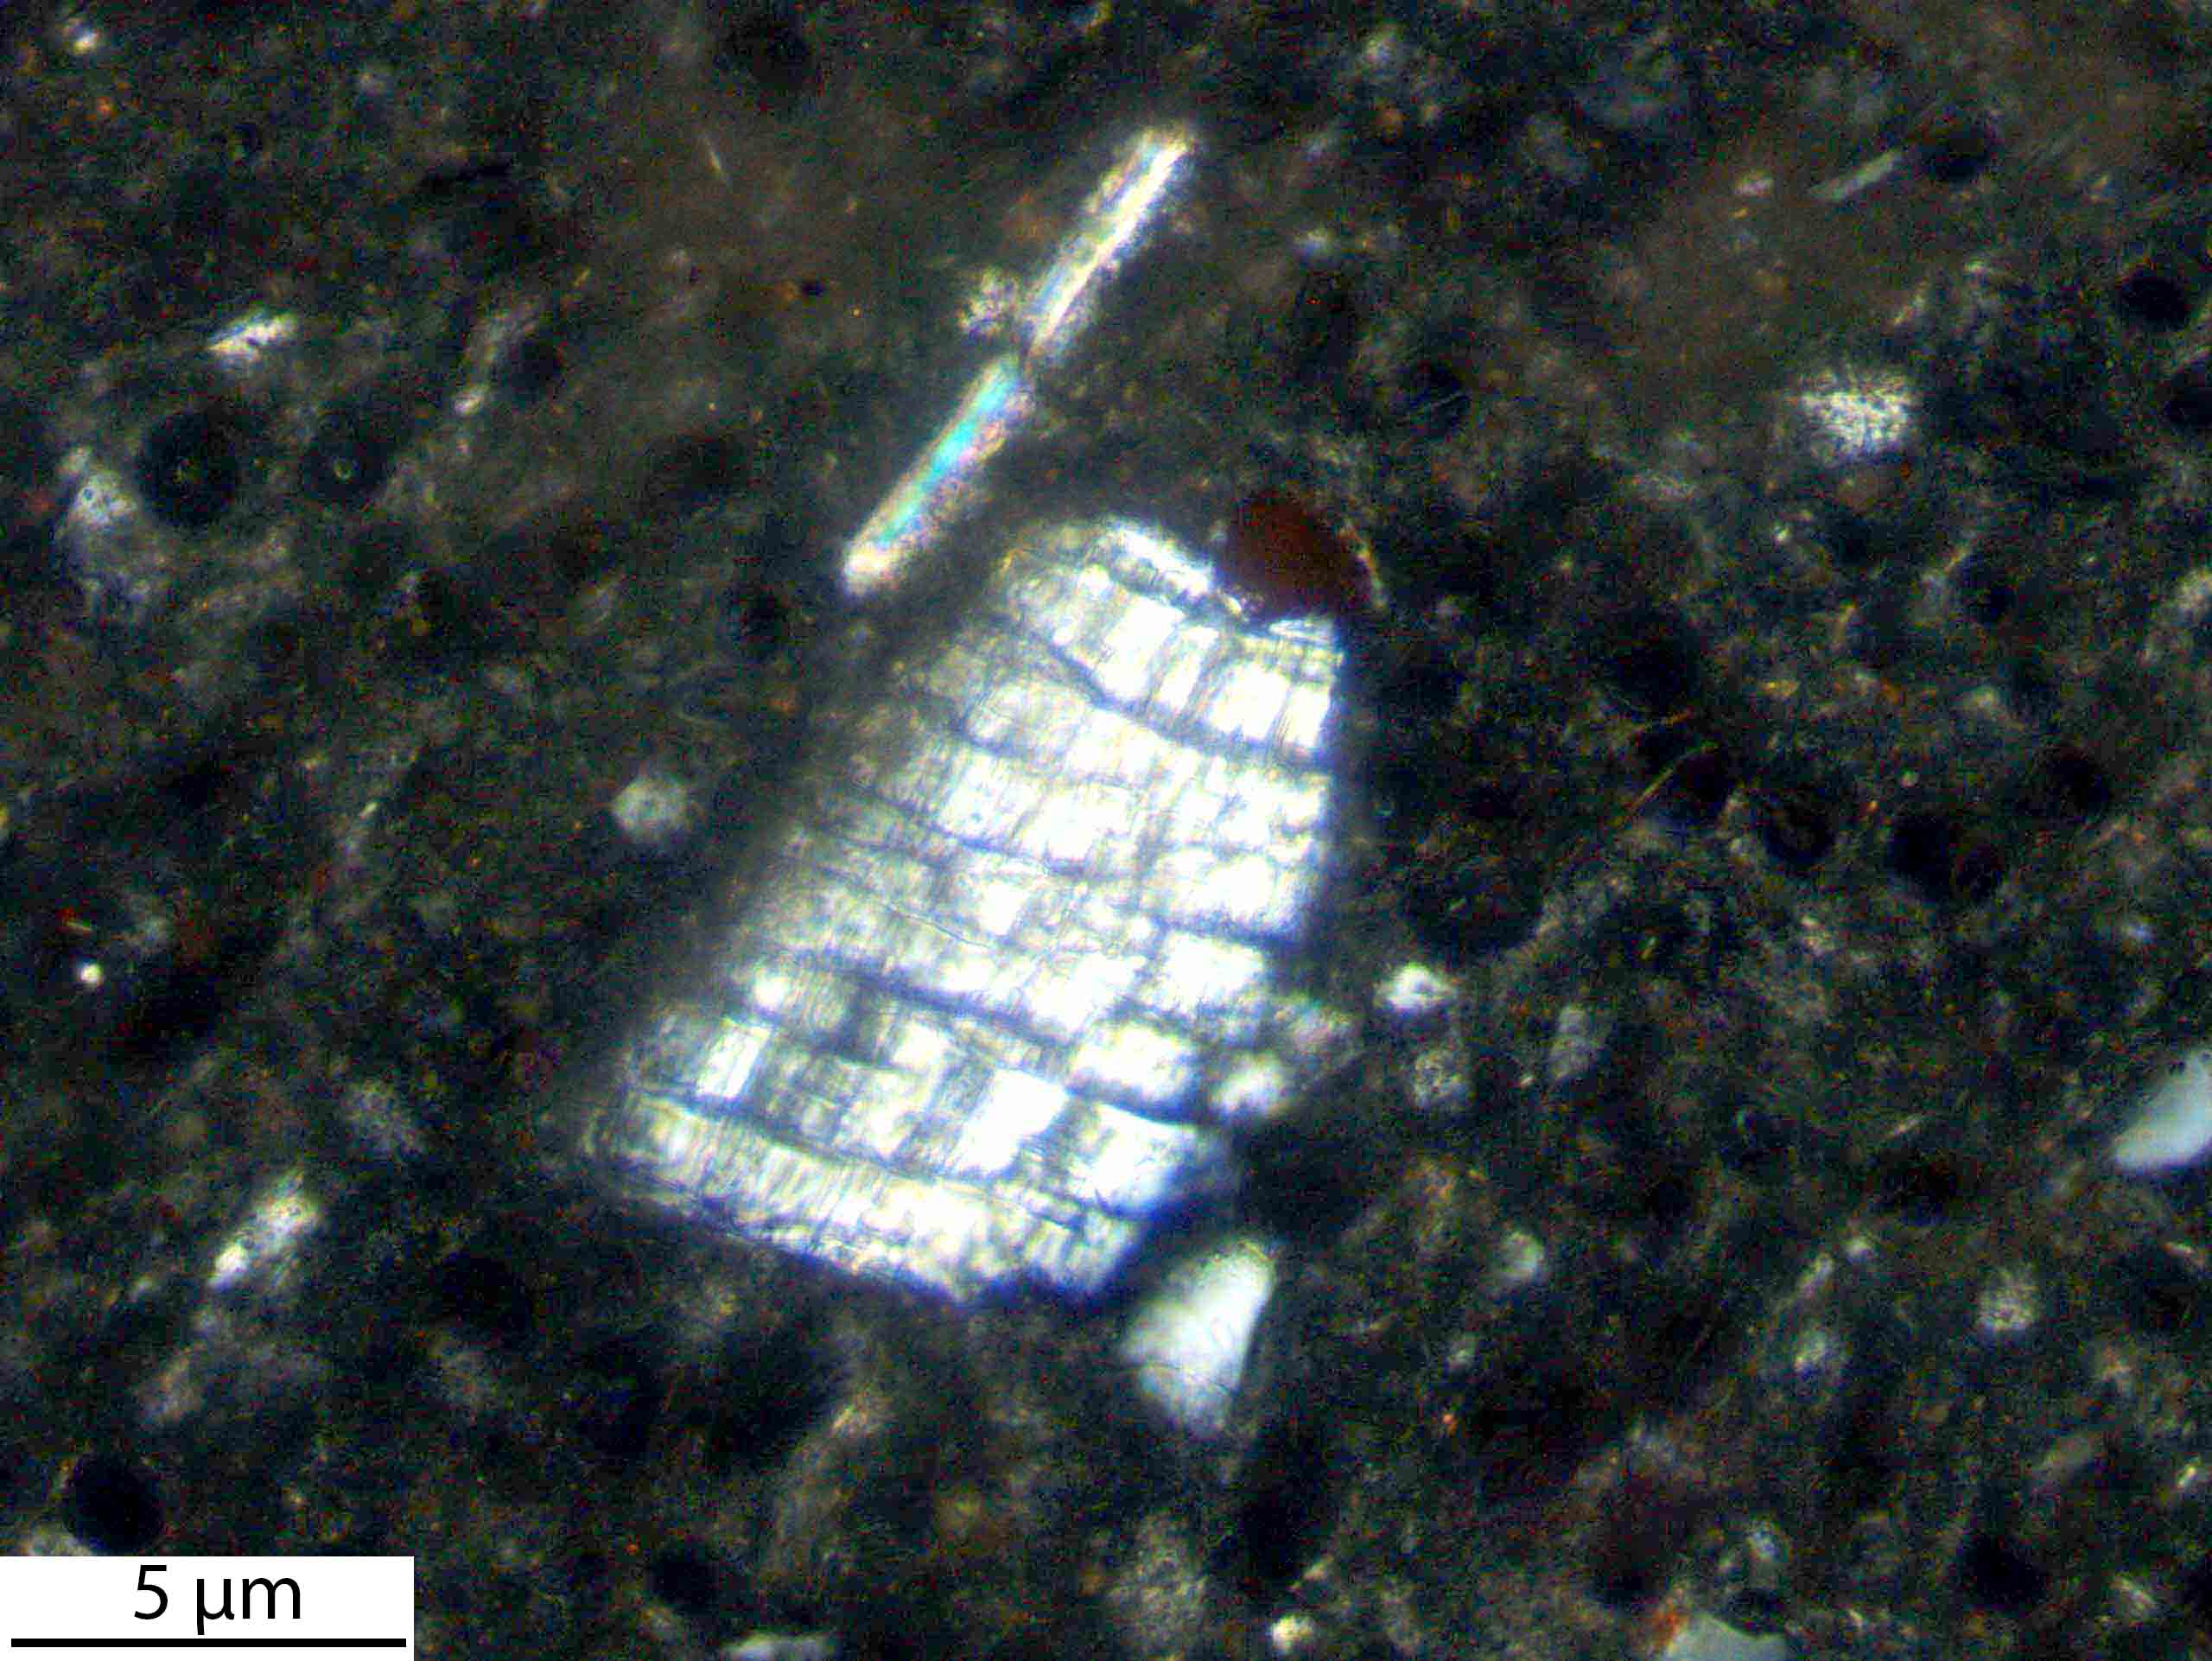
\includegraphics[width=\textwidth]{ThinSections/4-2_40x_XPL.jpg}
		\caption{Kyanite \& muscovite [XPL]}
	\end{subfigure}\hspace{.5em}\hfill
	\begin{subfigure}[t]{.24\textwidth}
		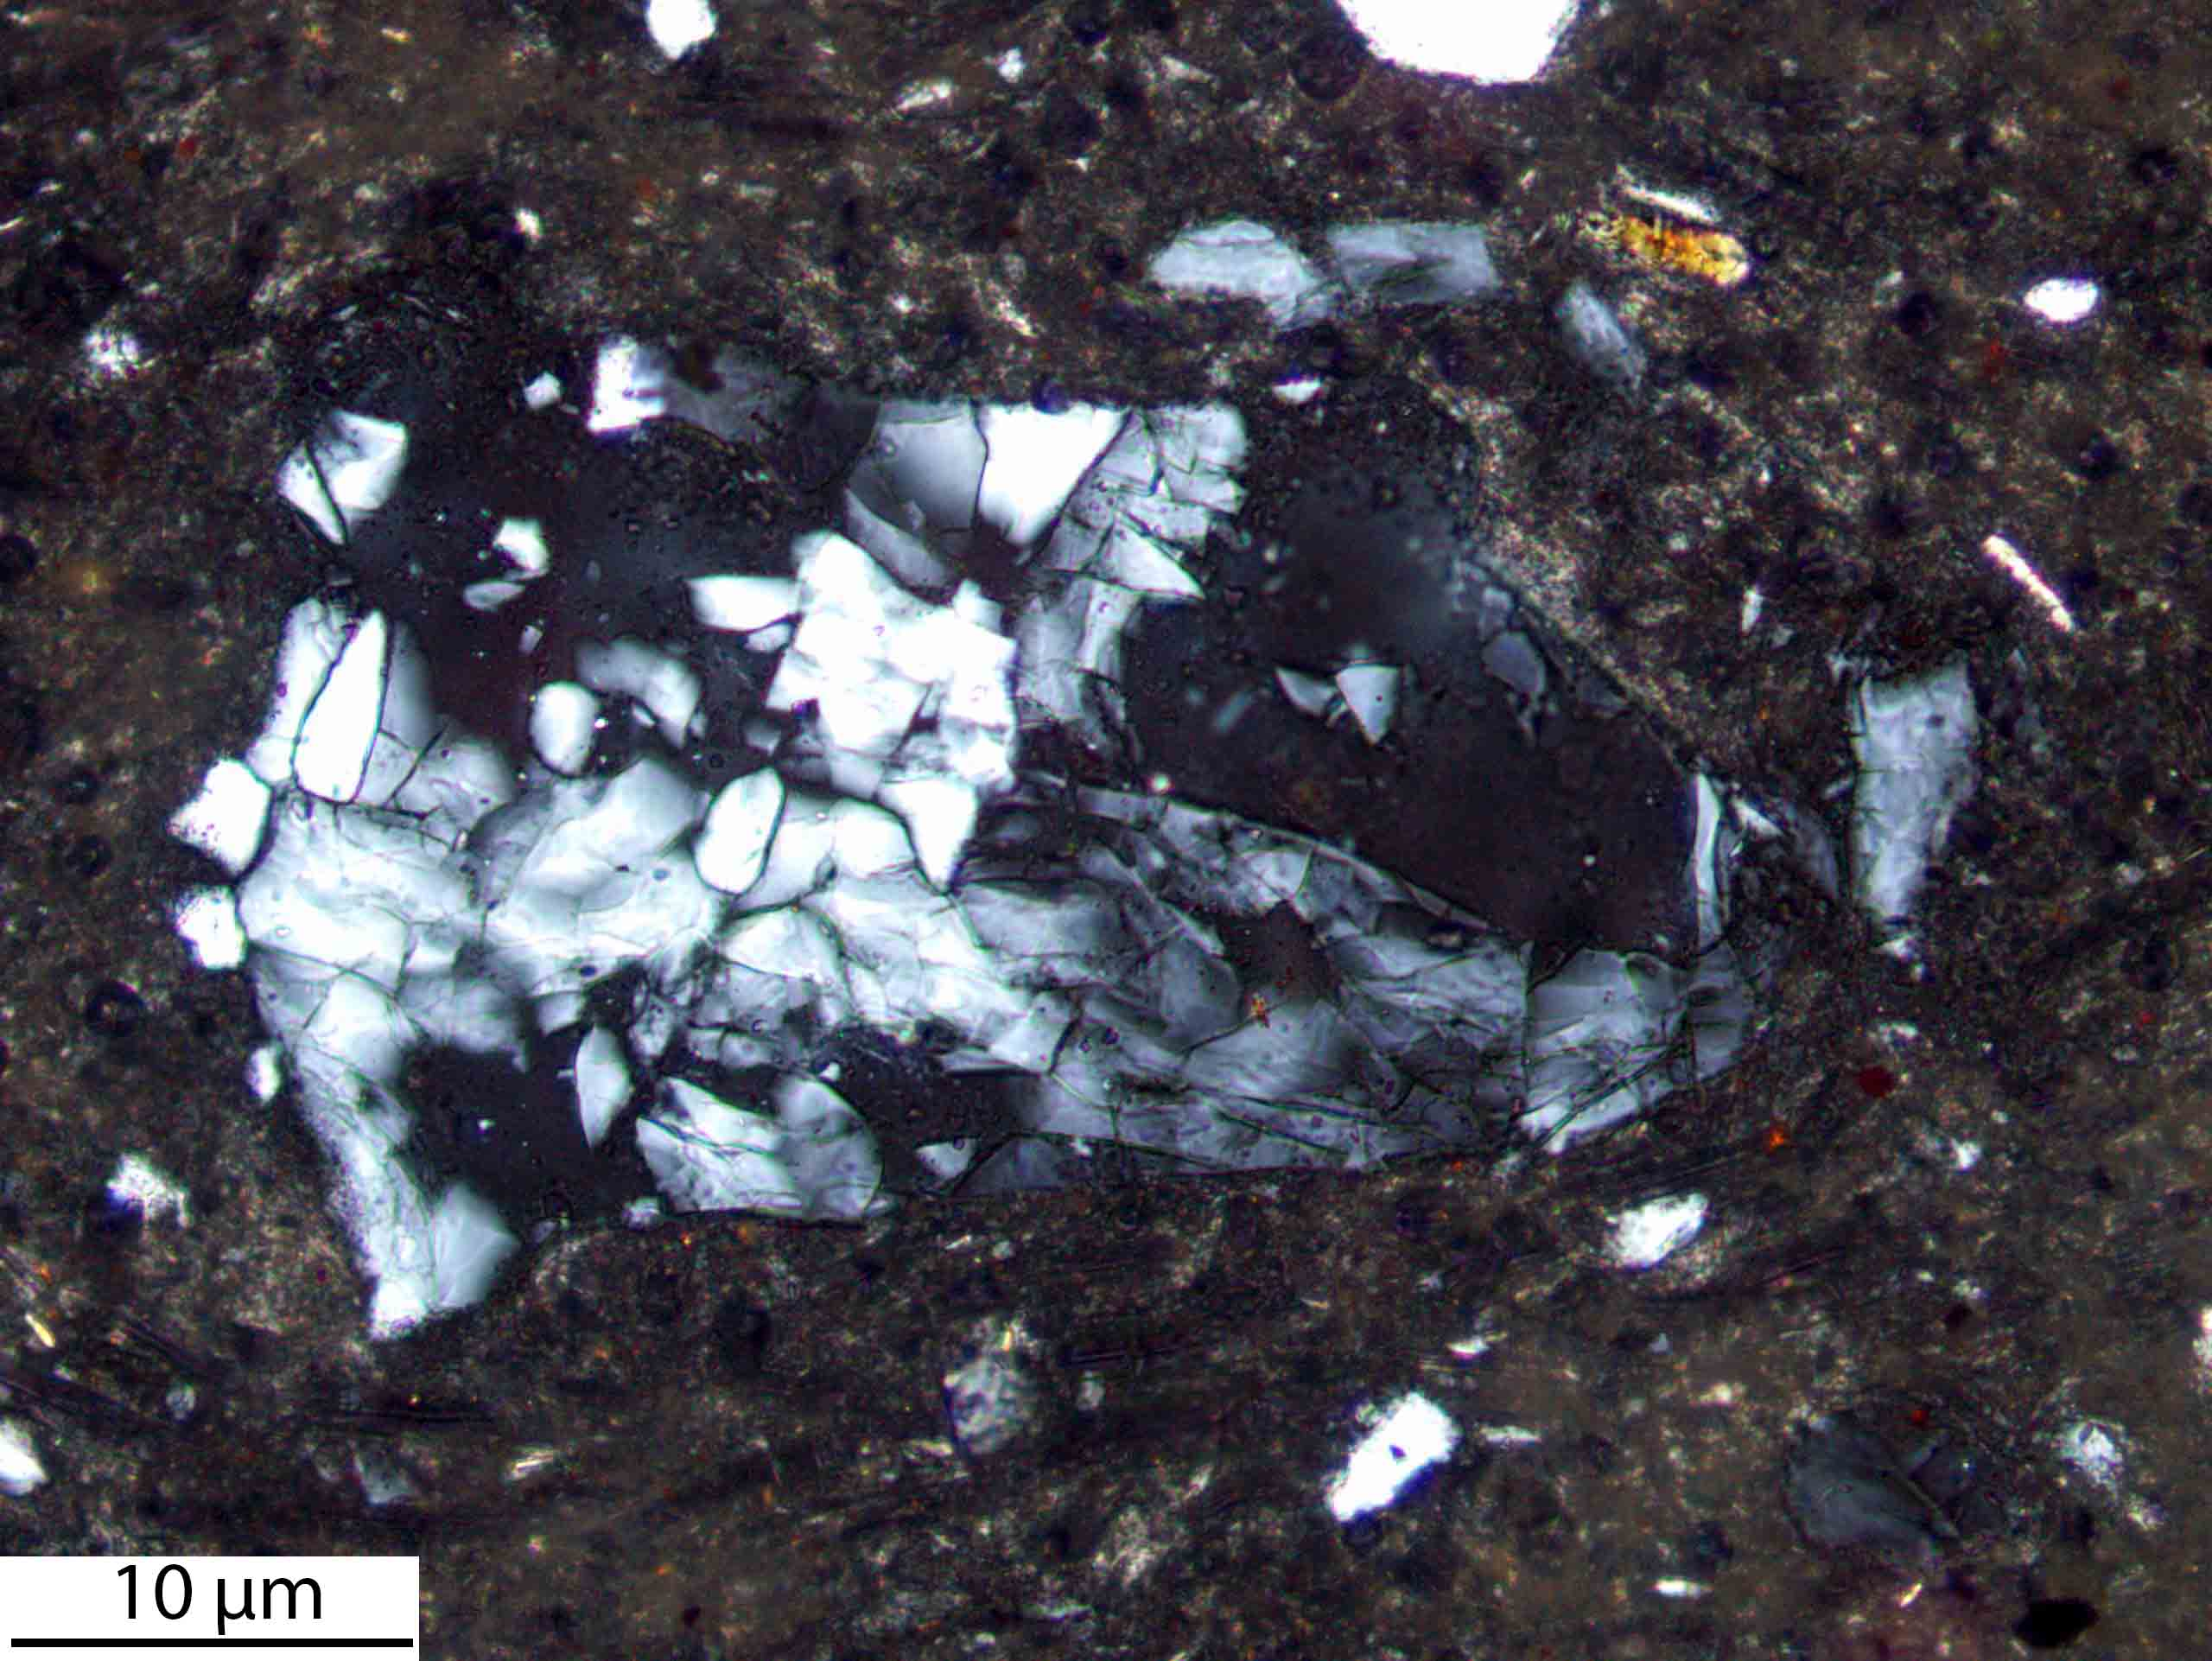
\includegraphics[width=\textwidth]{ThinSections/4-4_20x_XPL.jpg}
		\caption{Rock fragment [XPL]}
	\end{subfigure}\hspace{.1em}\hfill
%	\begin{subfigure}[t]{.24\textwidth}
%		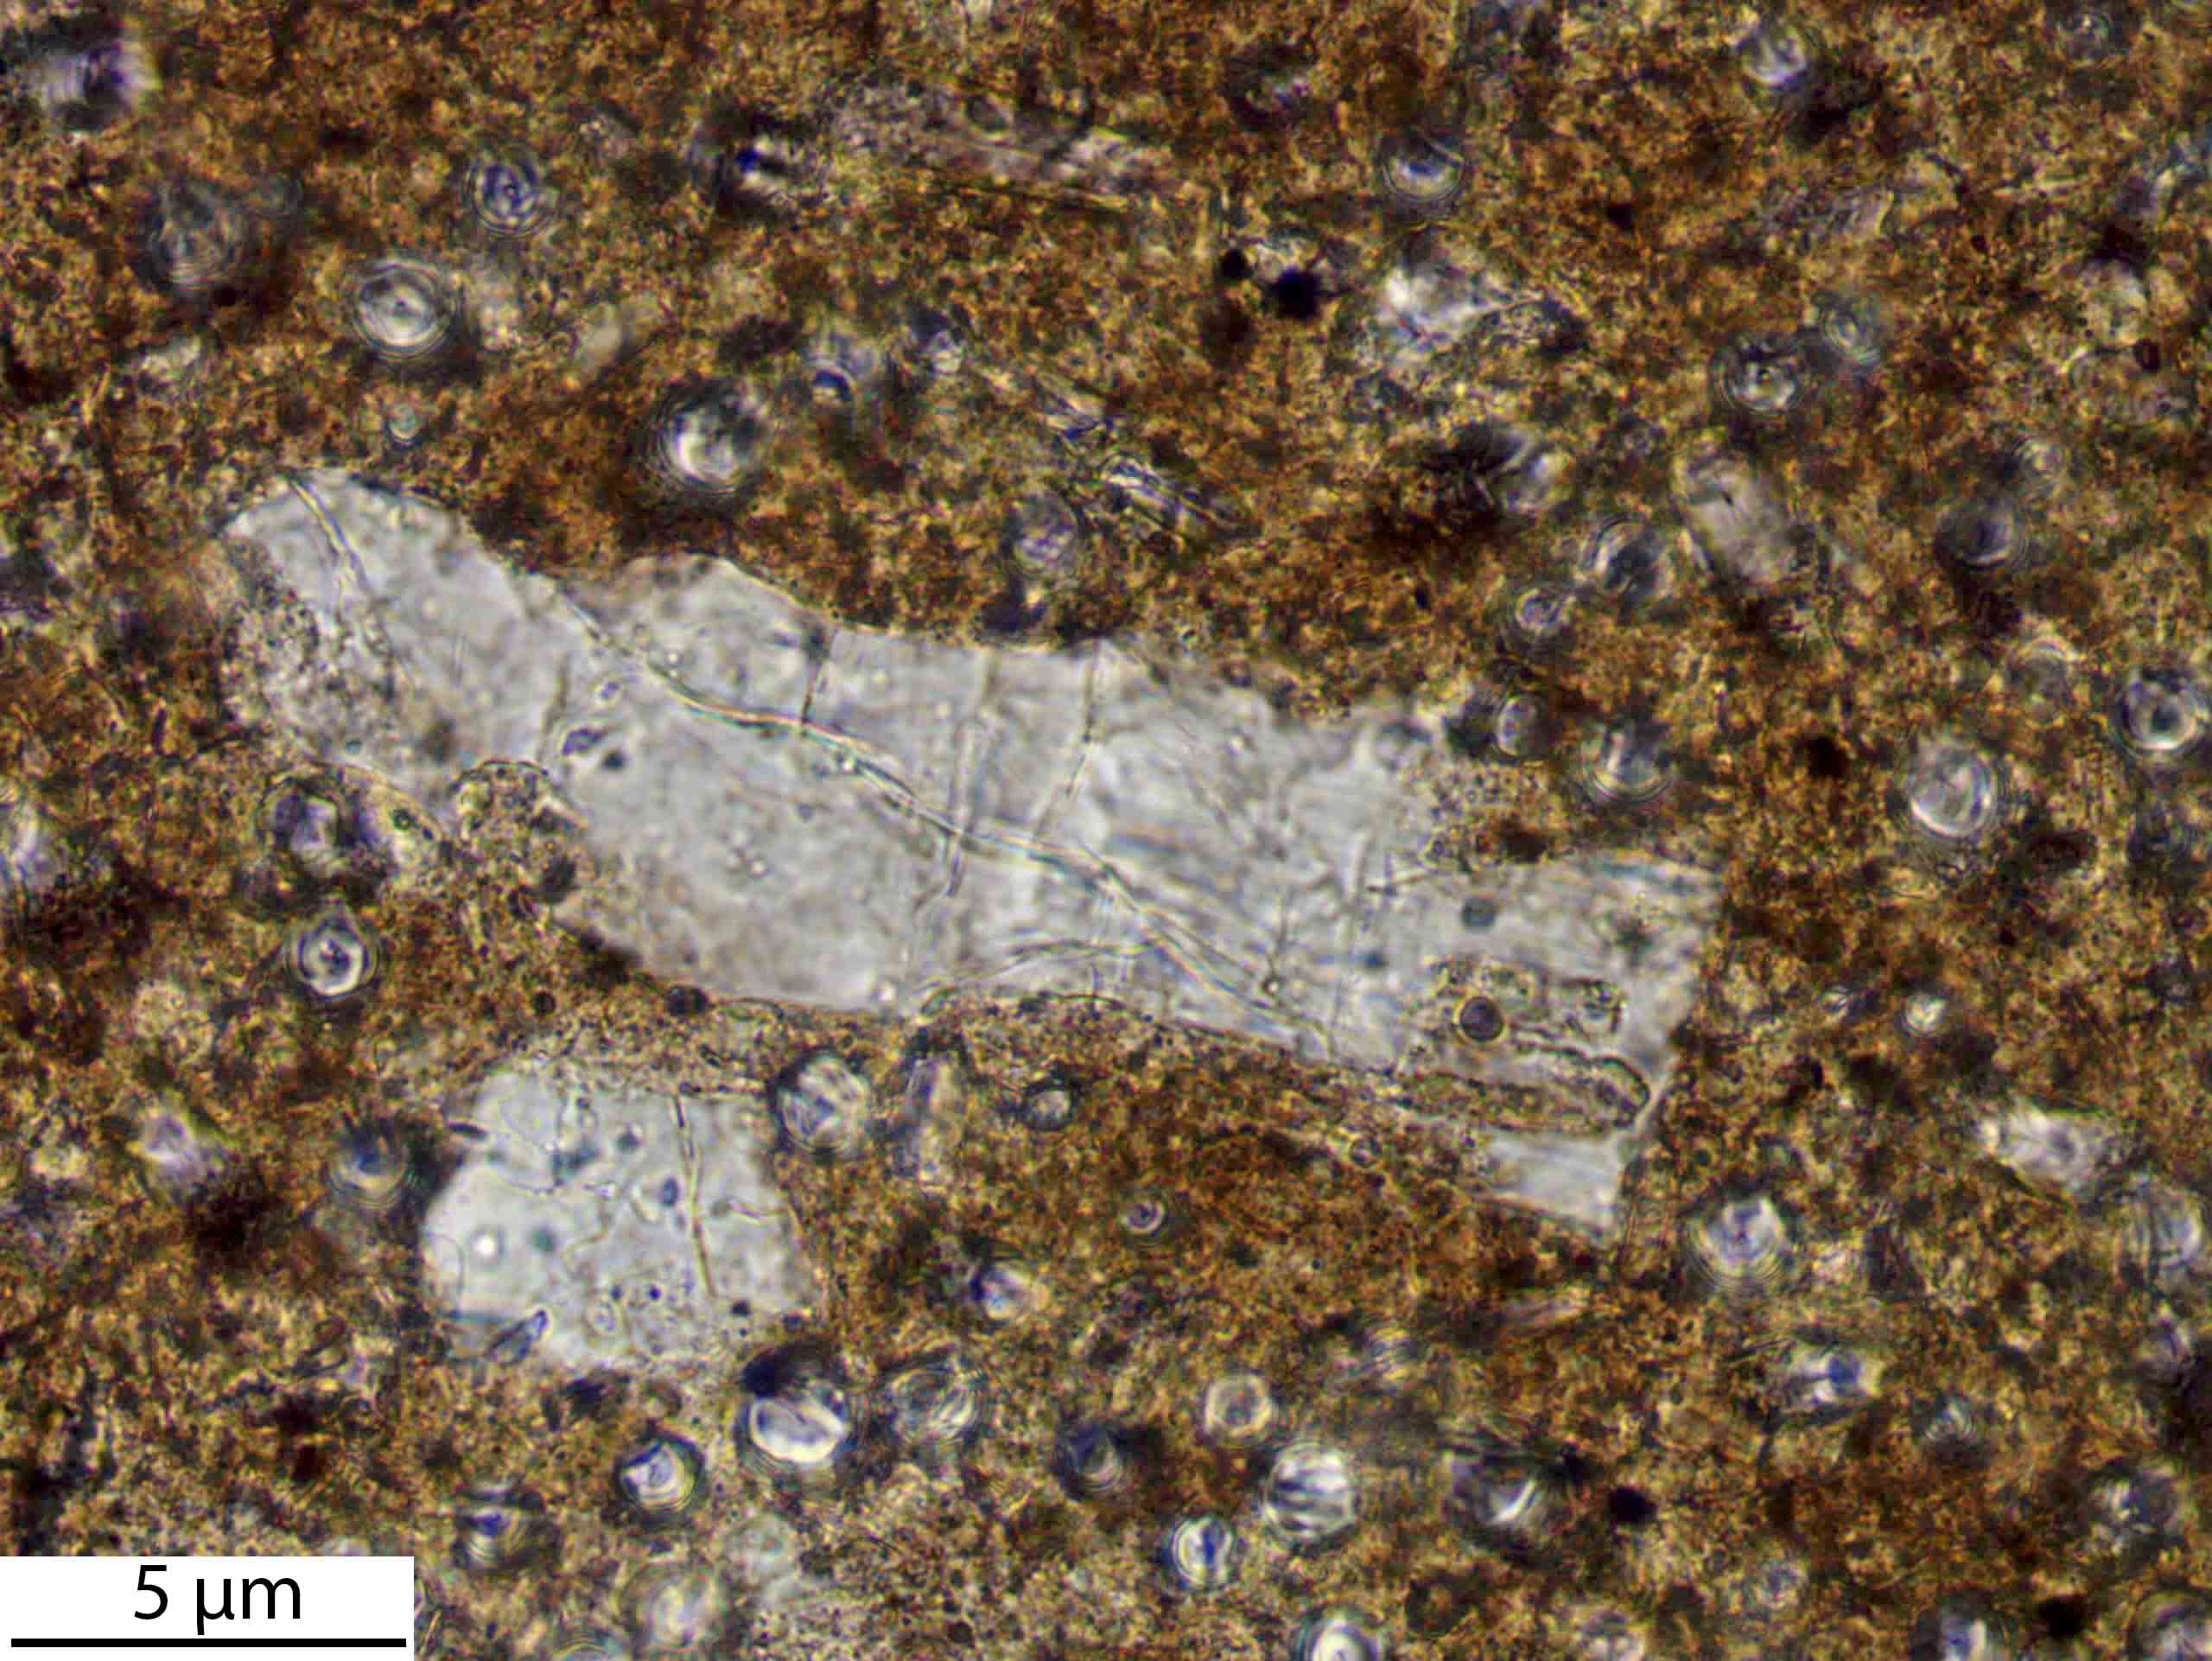
\includegraphics[width=\textwidth]{ThinSections/4-5_40x_PPL.jpg}
%		\caption{Plagioclase [PPL]}
%	\end{subfigure}\hspace{.1em}\hfill
	\begin{subfigure}[t]{.24\textwidth}
		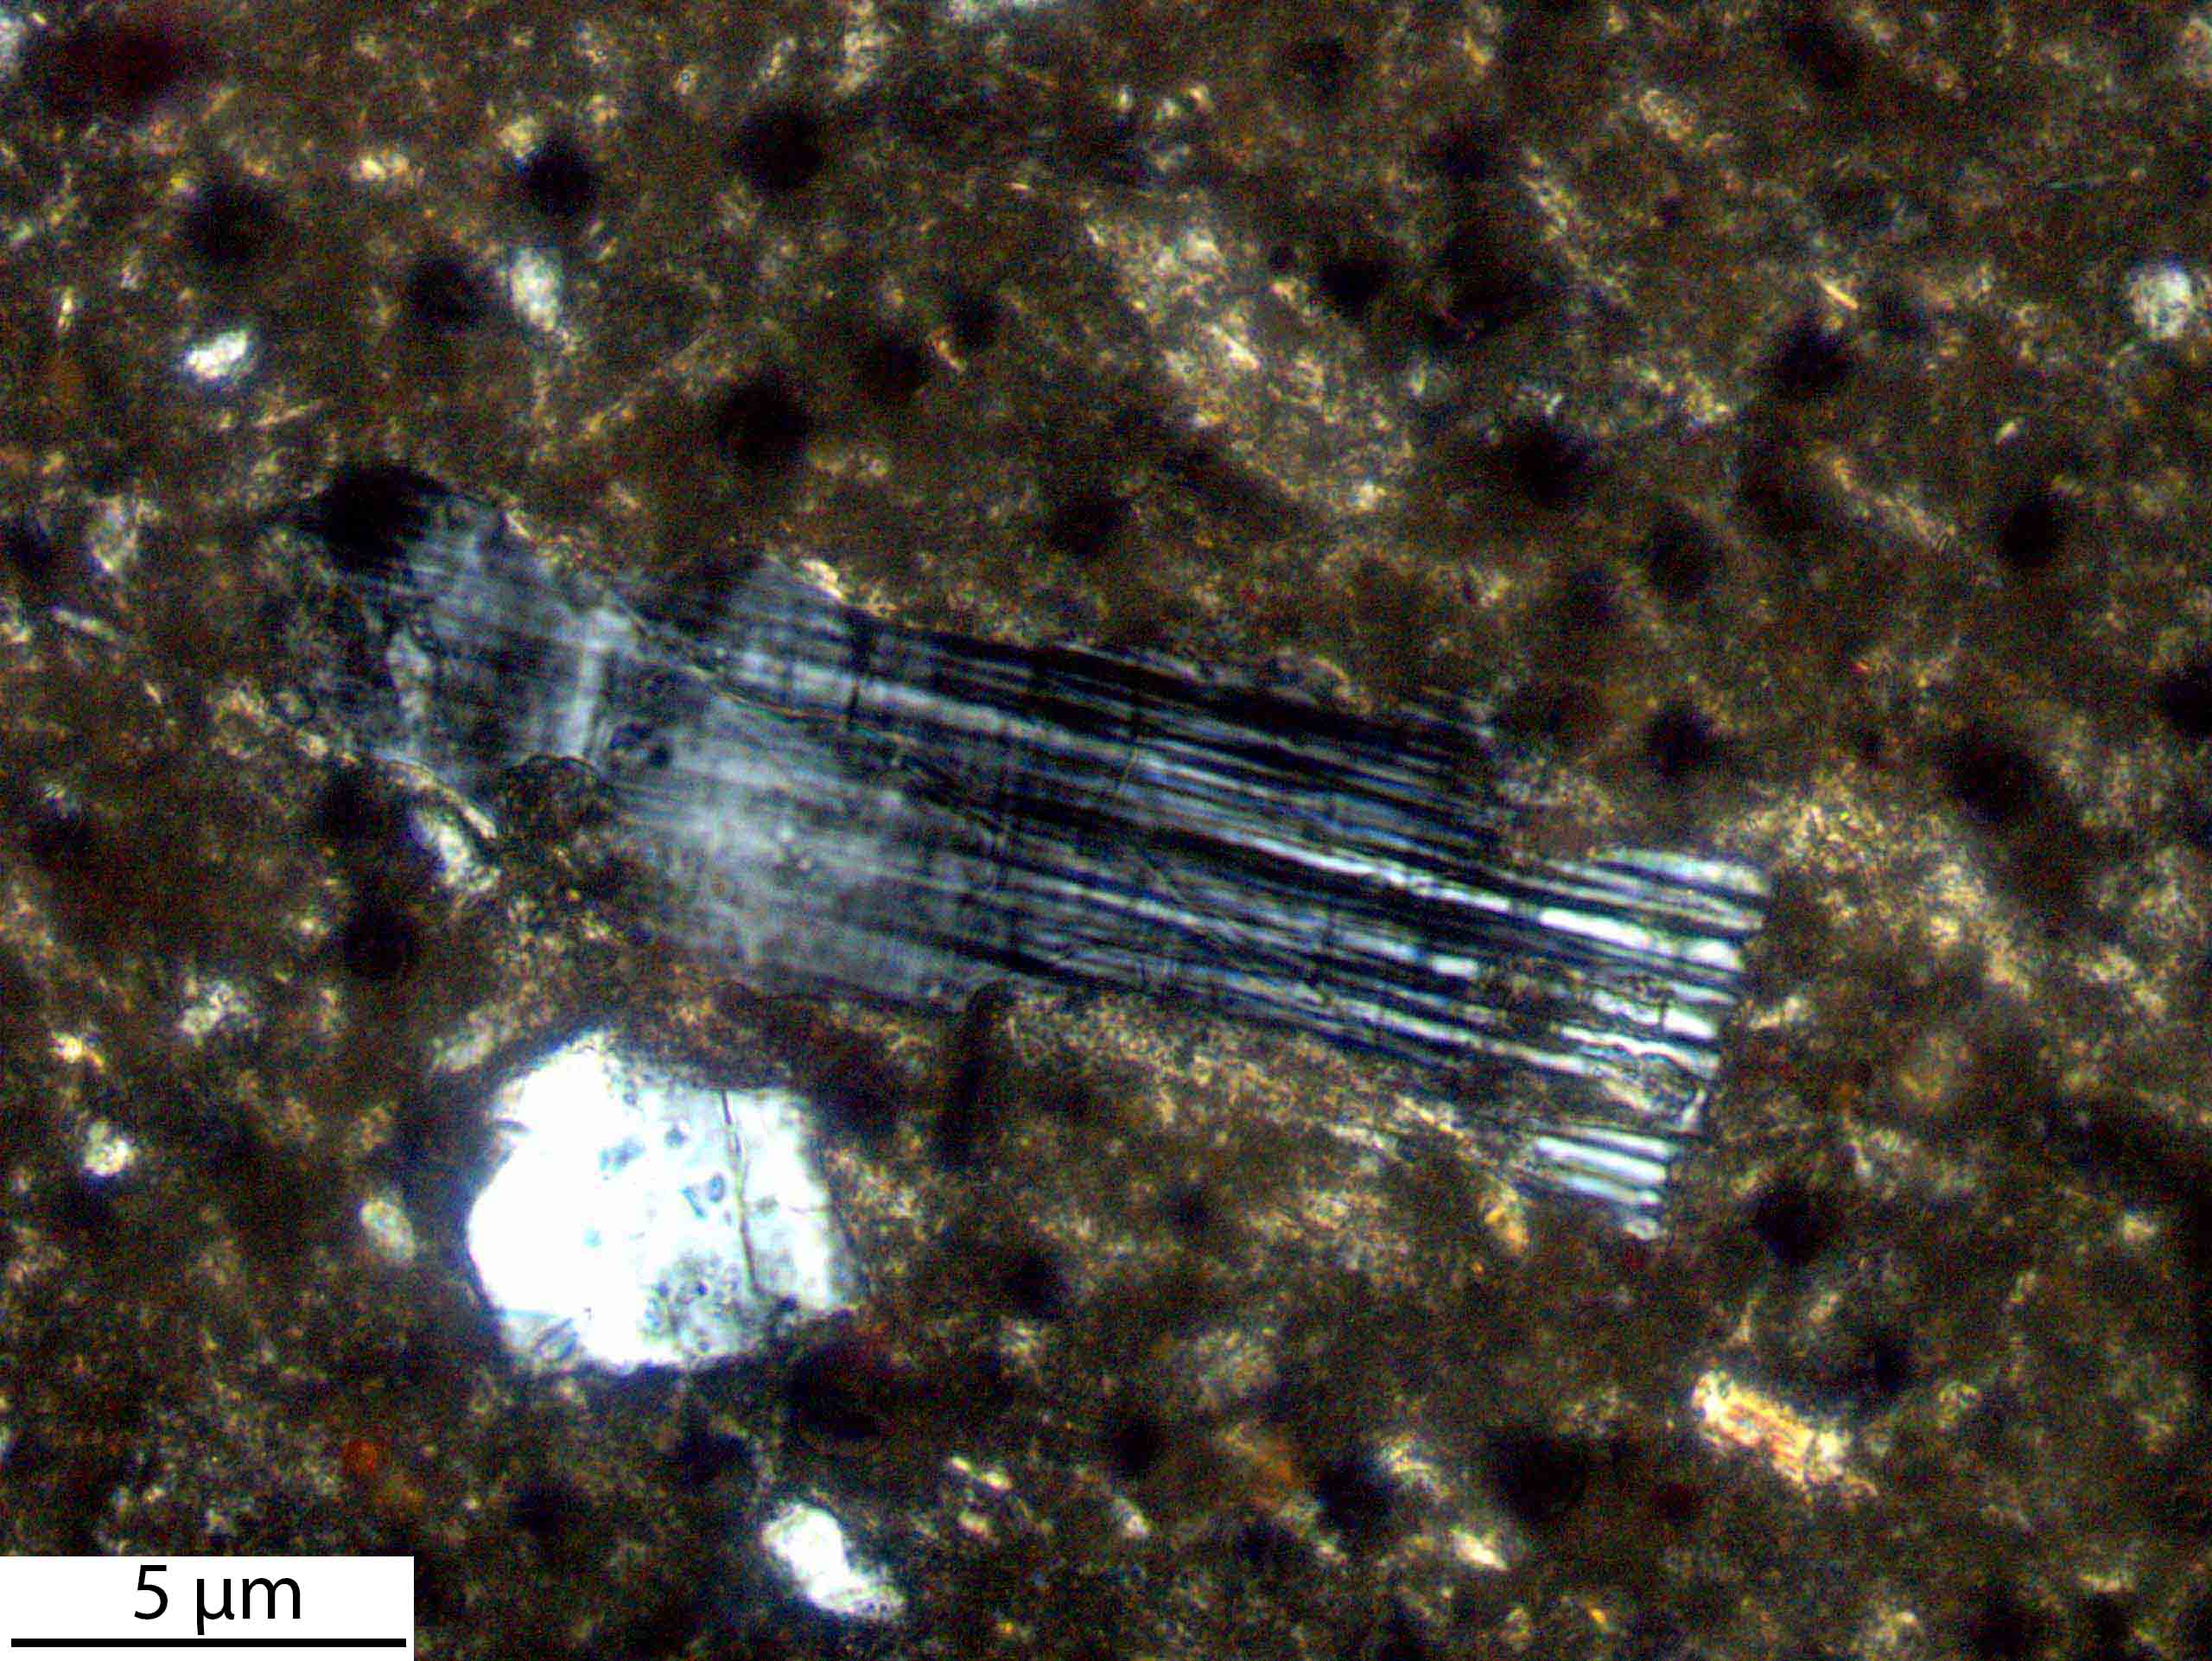
\includegraphics[width=\textwidth]{ThinSections/4-5_40x_XPL.jpg}
		\caption{Plagioclase [XPL]}
	\end{subfigure}
%	\begin{subfigure}[t]{.24\textwidth}
%		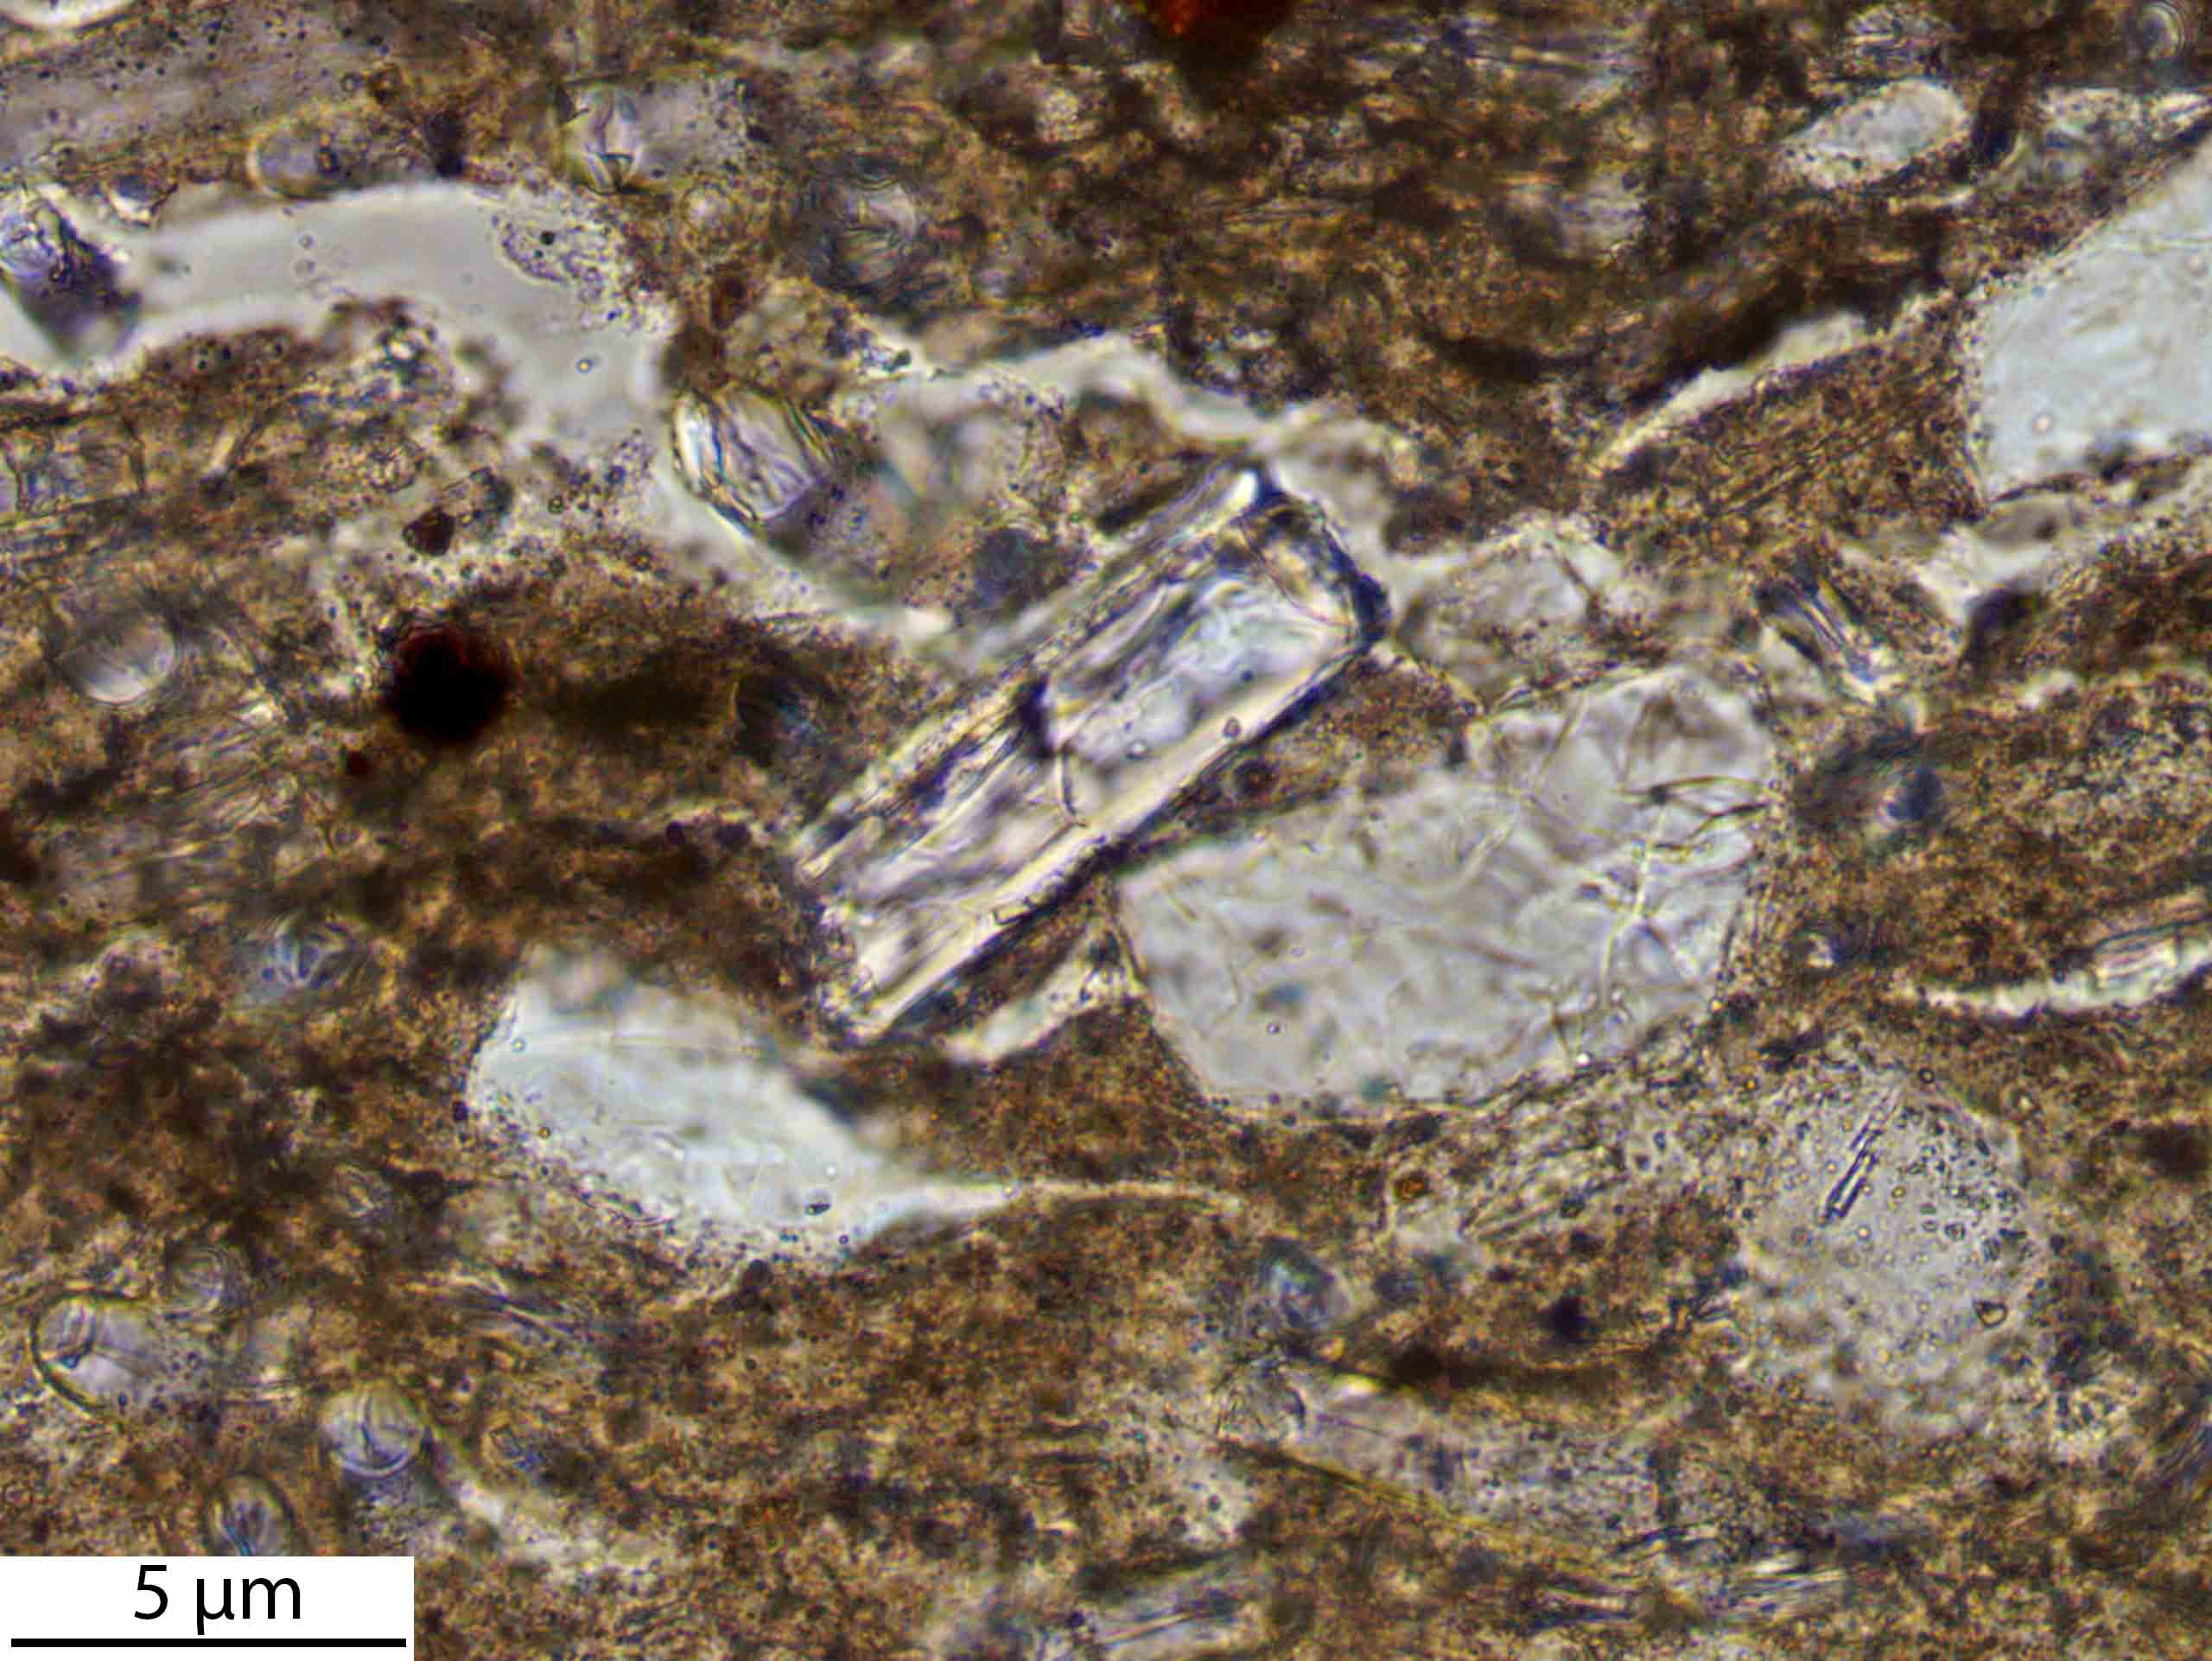
\includegraphics[width=\textwidth]{ThinSections/4-3_40x_PPL.jpg}
%		\caption{Zircone [PPL]}
%	\end{subfigure}\hspace{.1em}\hfill
%	\begin{subfigure}[t]{.24\textwidth}
%		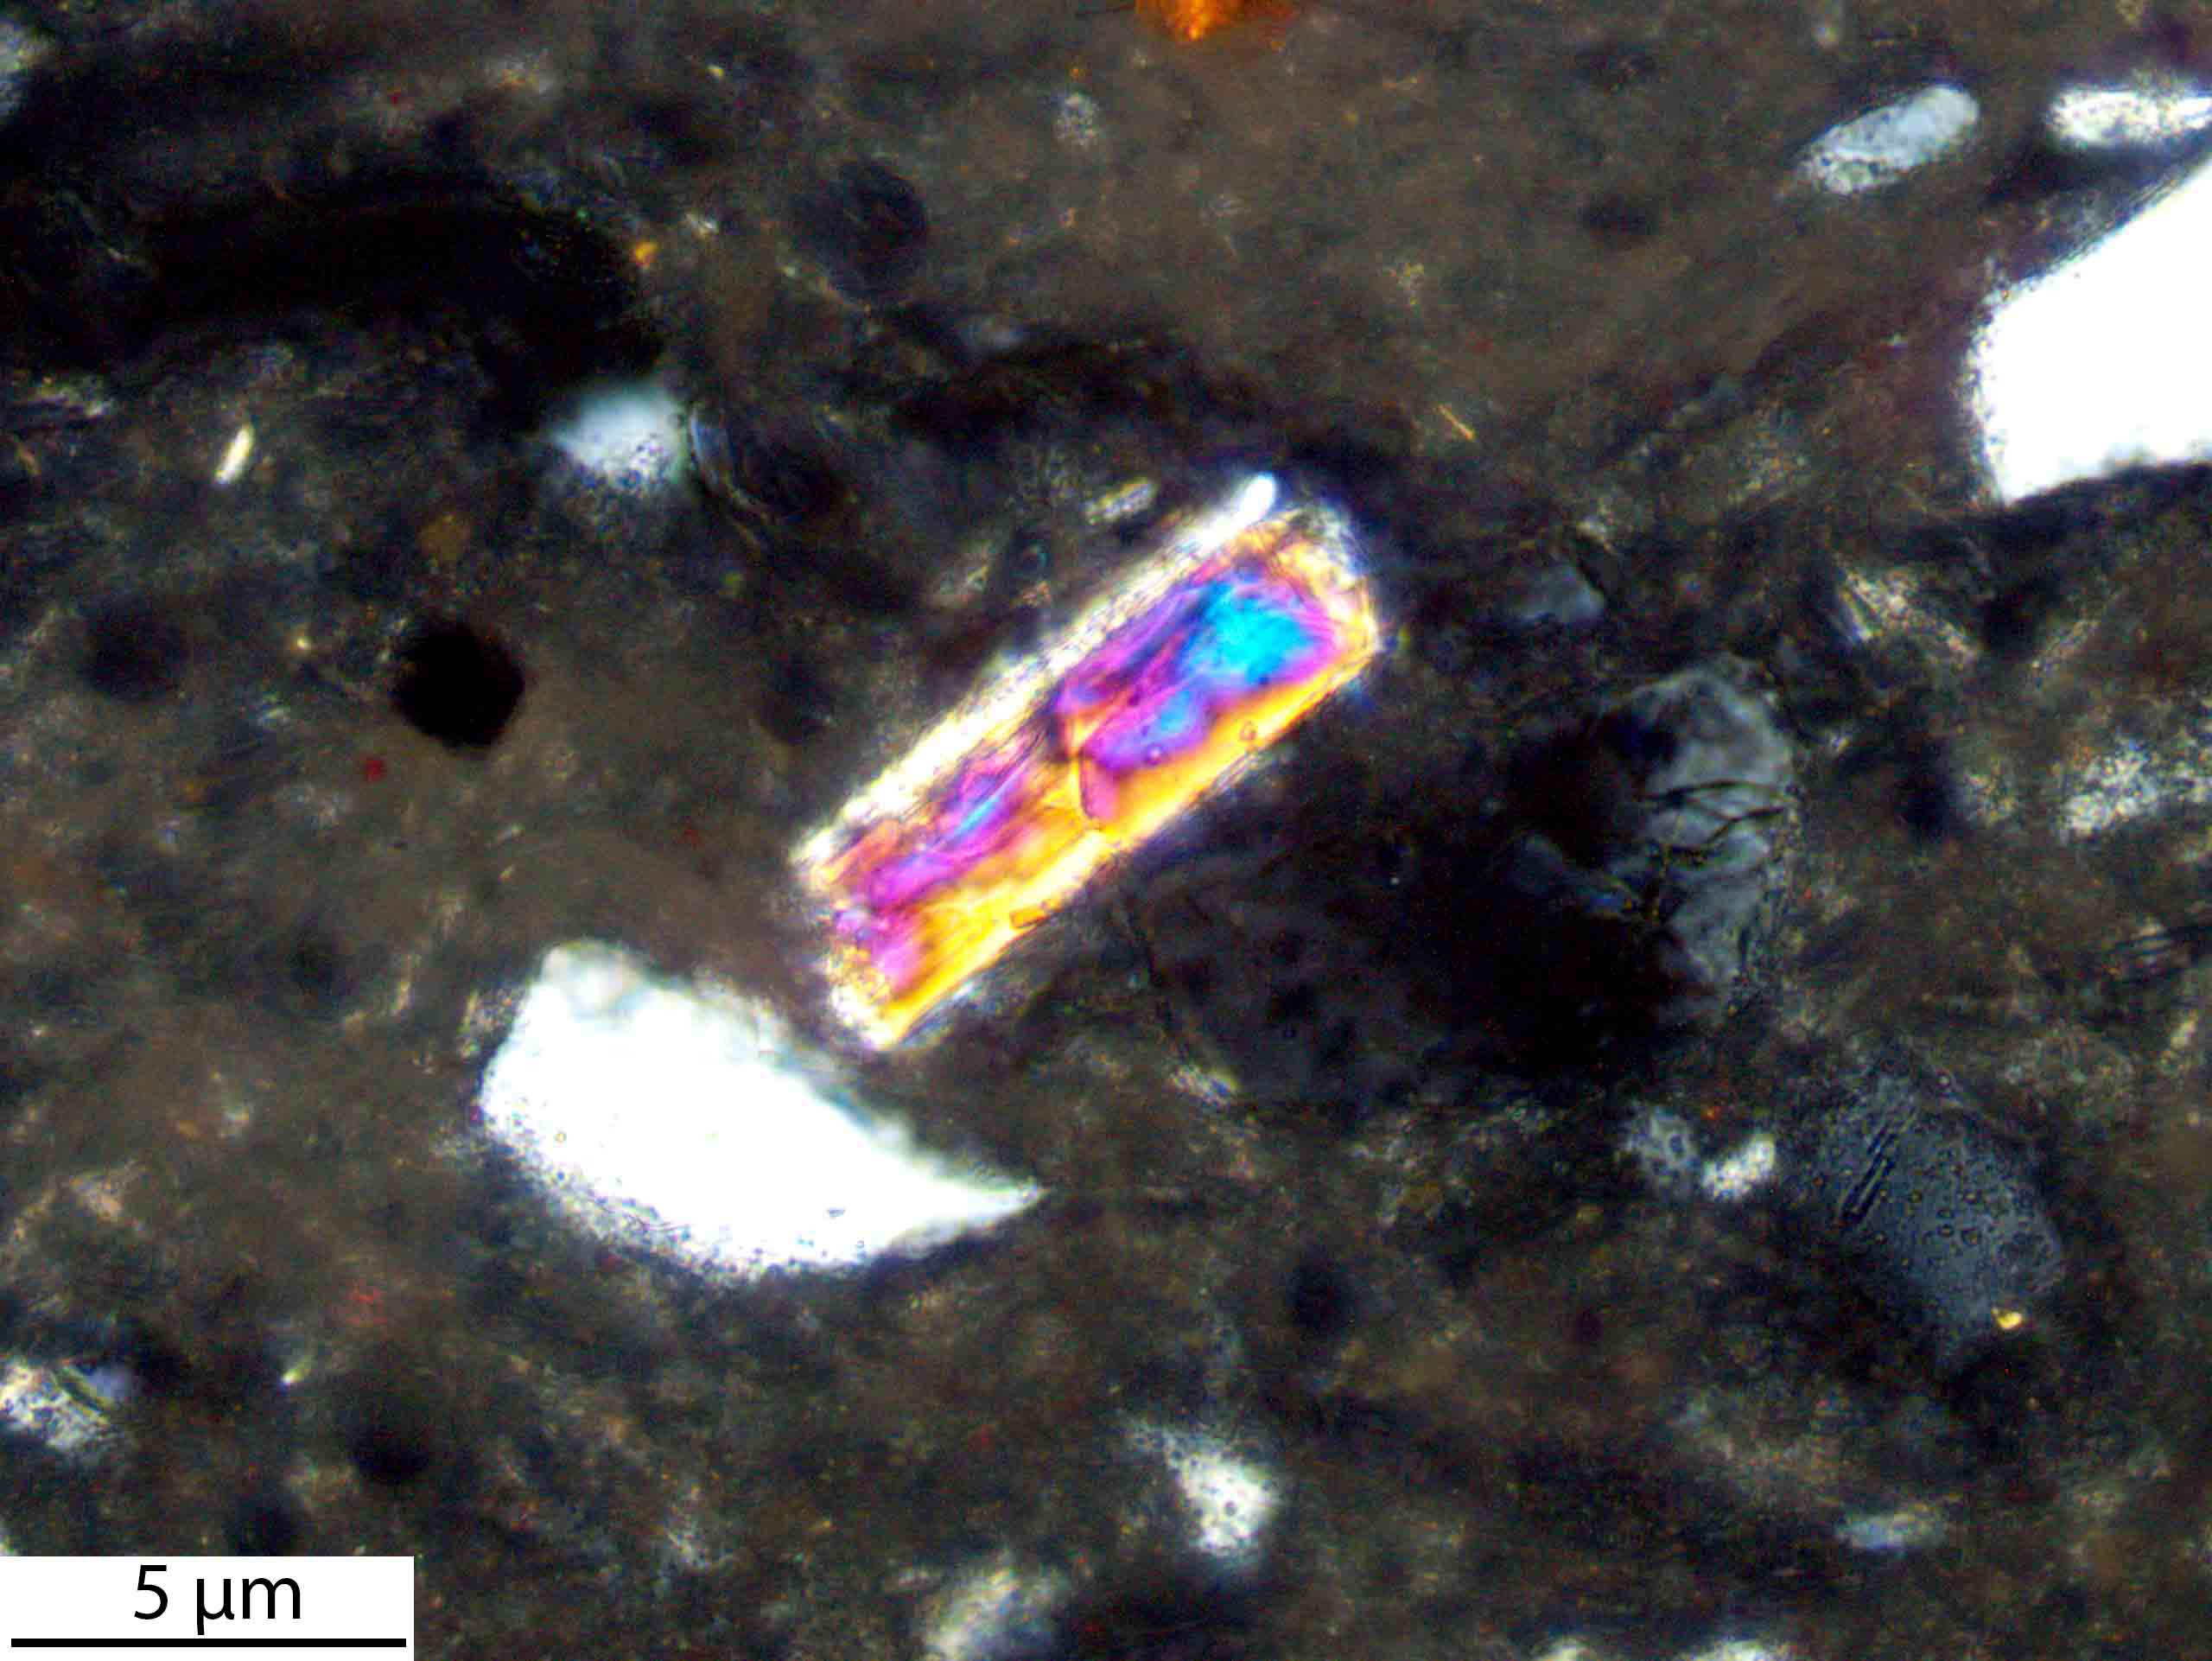
\includegraphics[width=\textwidth]{ThinSections/4-3_40x_XPL.jpg}
%		\caption{Zircone [XPL]}
%	\end{subfigure}	
	\caption{}
	\label{fig:4_pik}
\end{figure}

\newpage\subsection{PIK~87/1-8:1 \citep[pik\#5; Fig.~\ref{fig:pik.pottery}.6; cf. Ngbanja style;][428 Pl.~47.20]{Seidensticker.2021e}}

\begin{multicols}{2}
\noindent The section shows a homogeneous non-calcareous, iron-rich fine fraction (dark brown [PPL]) with undifferentiated b-fabric. Secondary calcite is visible on all pores and around the elements of the coarse fraction. Voids are -- relative to the plane of the section -- oriented U-shaped in one part and wall-parallel in the other. This is regarded as indication for a shaping via coiling. The coarse fractions is characterized by sub-angular quartz in  a bimodal grain-size distribution. Also present is muscovite and occasionally zircon (c--d). The c/f-related distribution pattern is single-spaced porphyric.
\end{multicols}

% (secondary) calcite around every pore and mineral

%\vfill
\begin{figure}[H]
	\centering
	\begin{subfigure}[t]{.49\textwidth}
		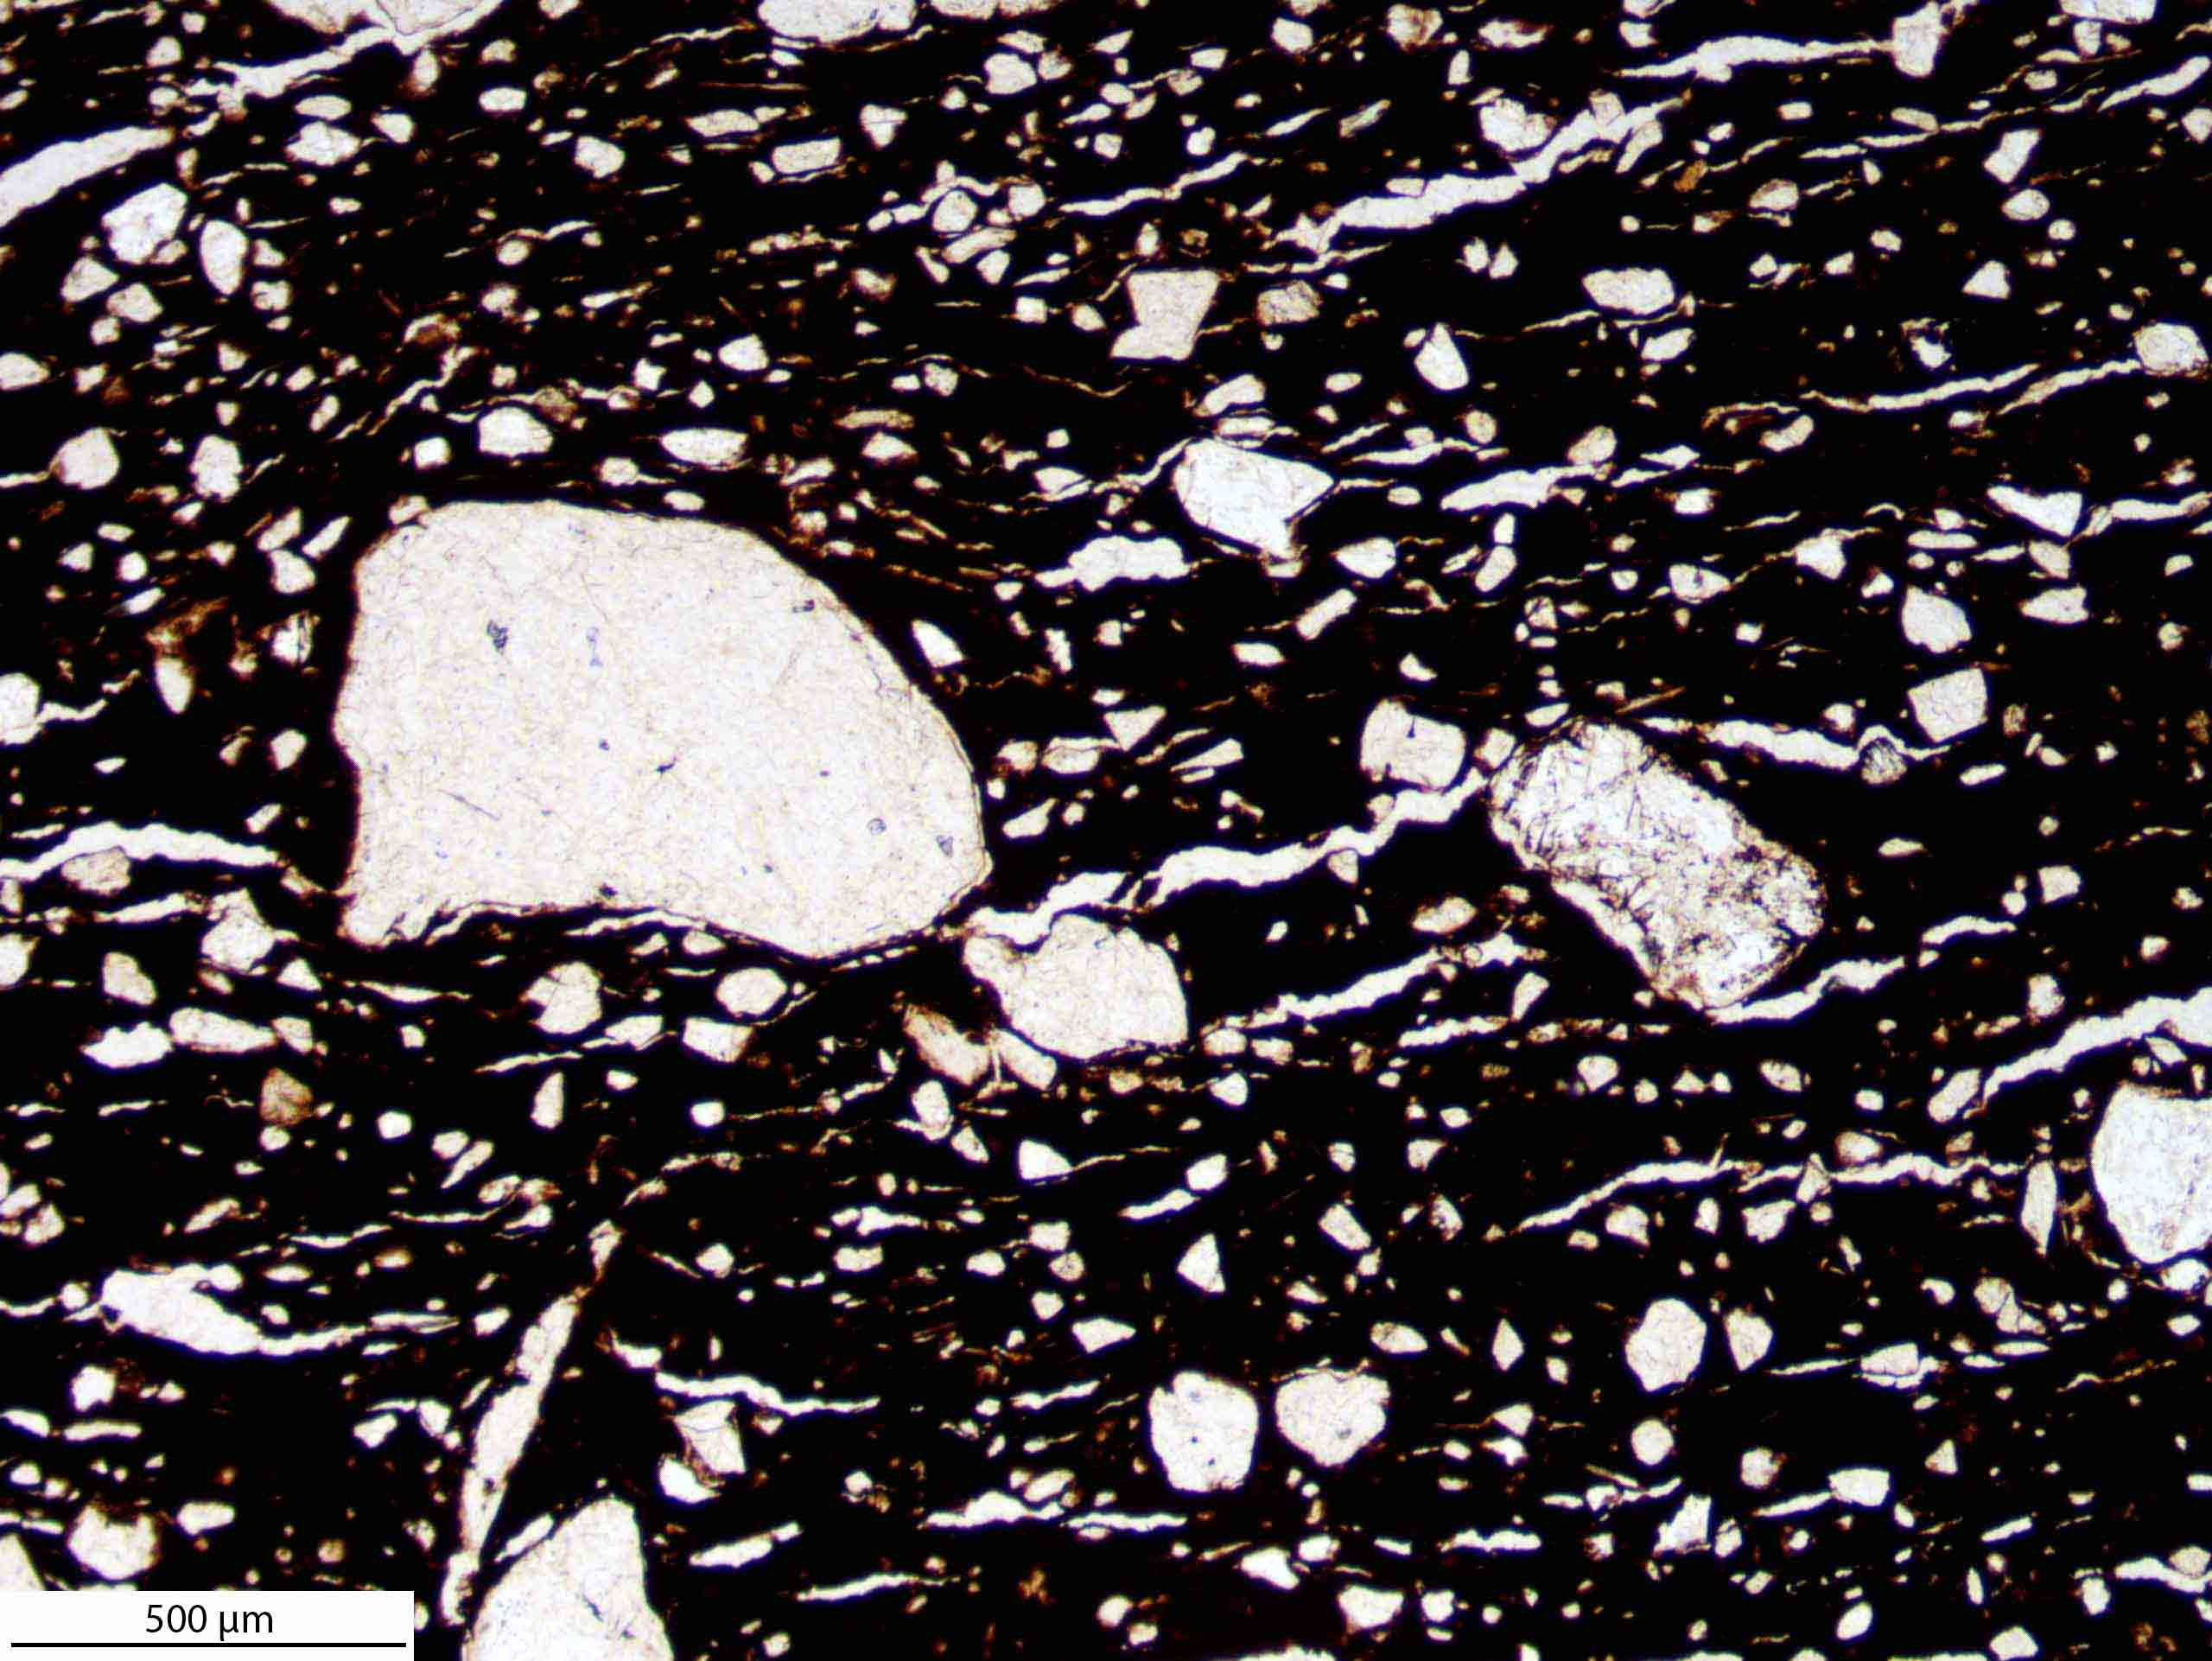
\includegraphics[width=\textwidth]{ThinSections/5-1_4x_PPL.jpg}
		\caption{[PPL]}
	\end{subfigure}\hspace{.5em}\hfill
	\begin{subfigure}[t]{.49\textwidth}
		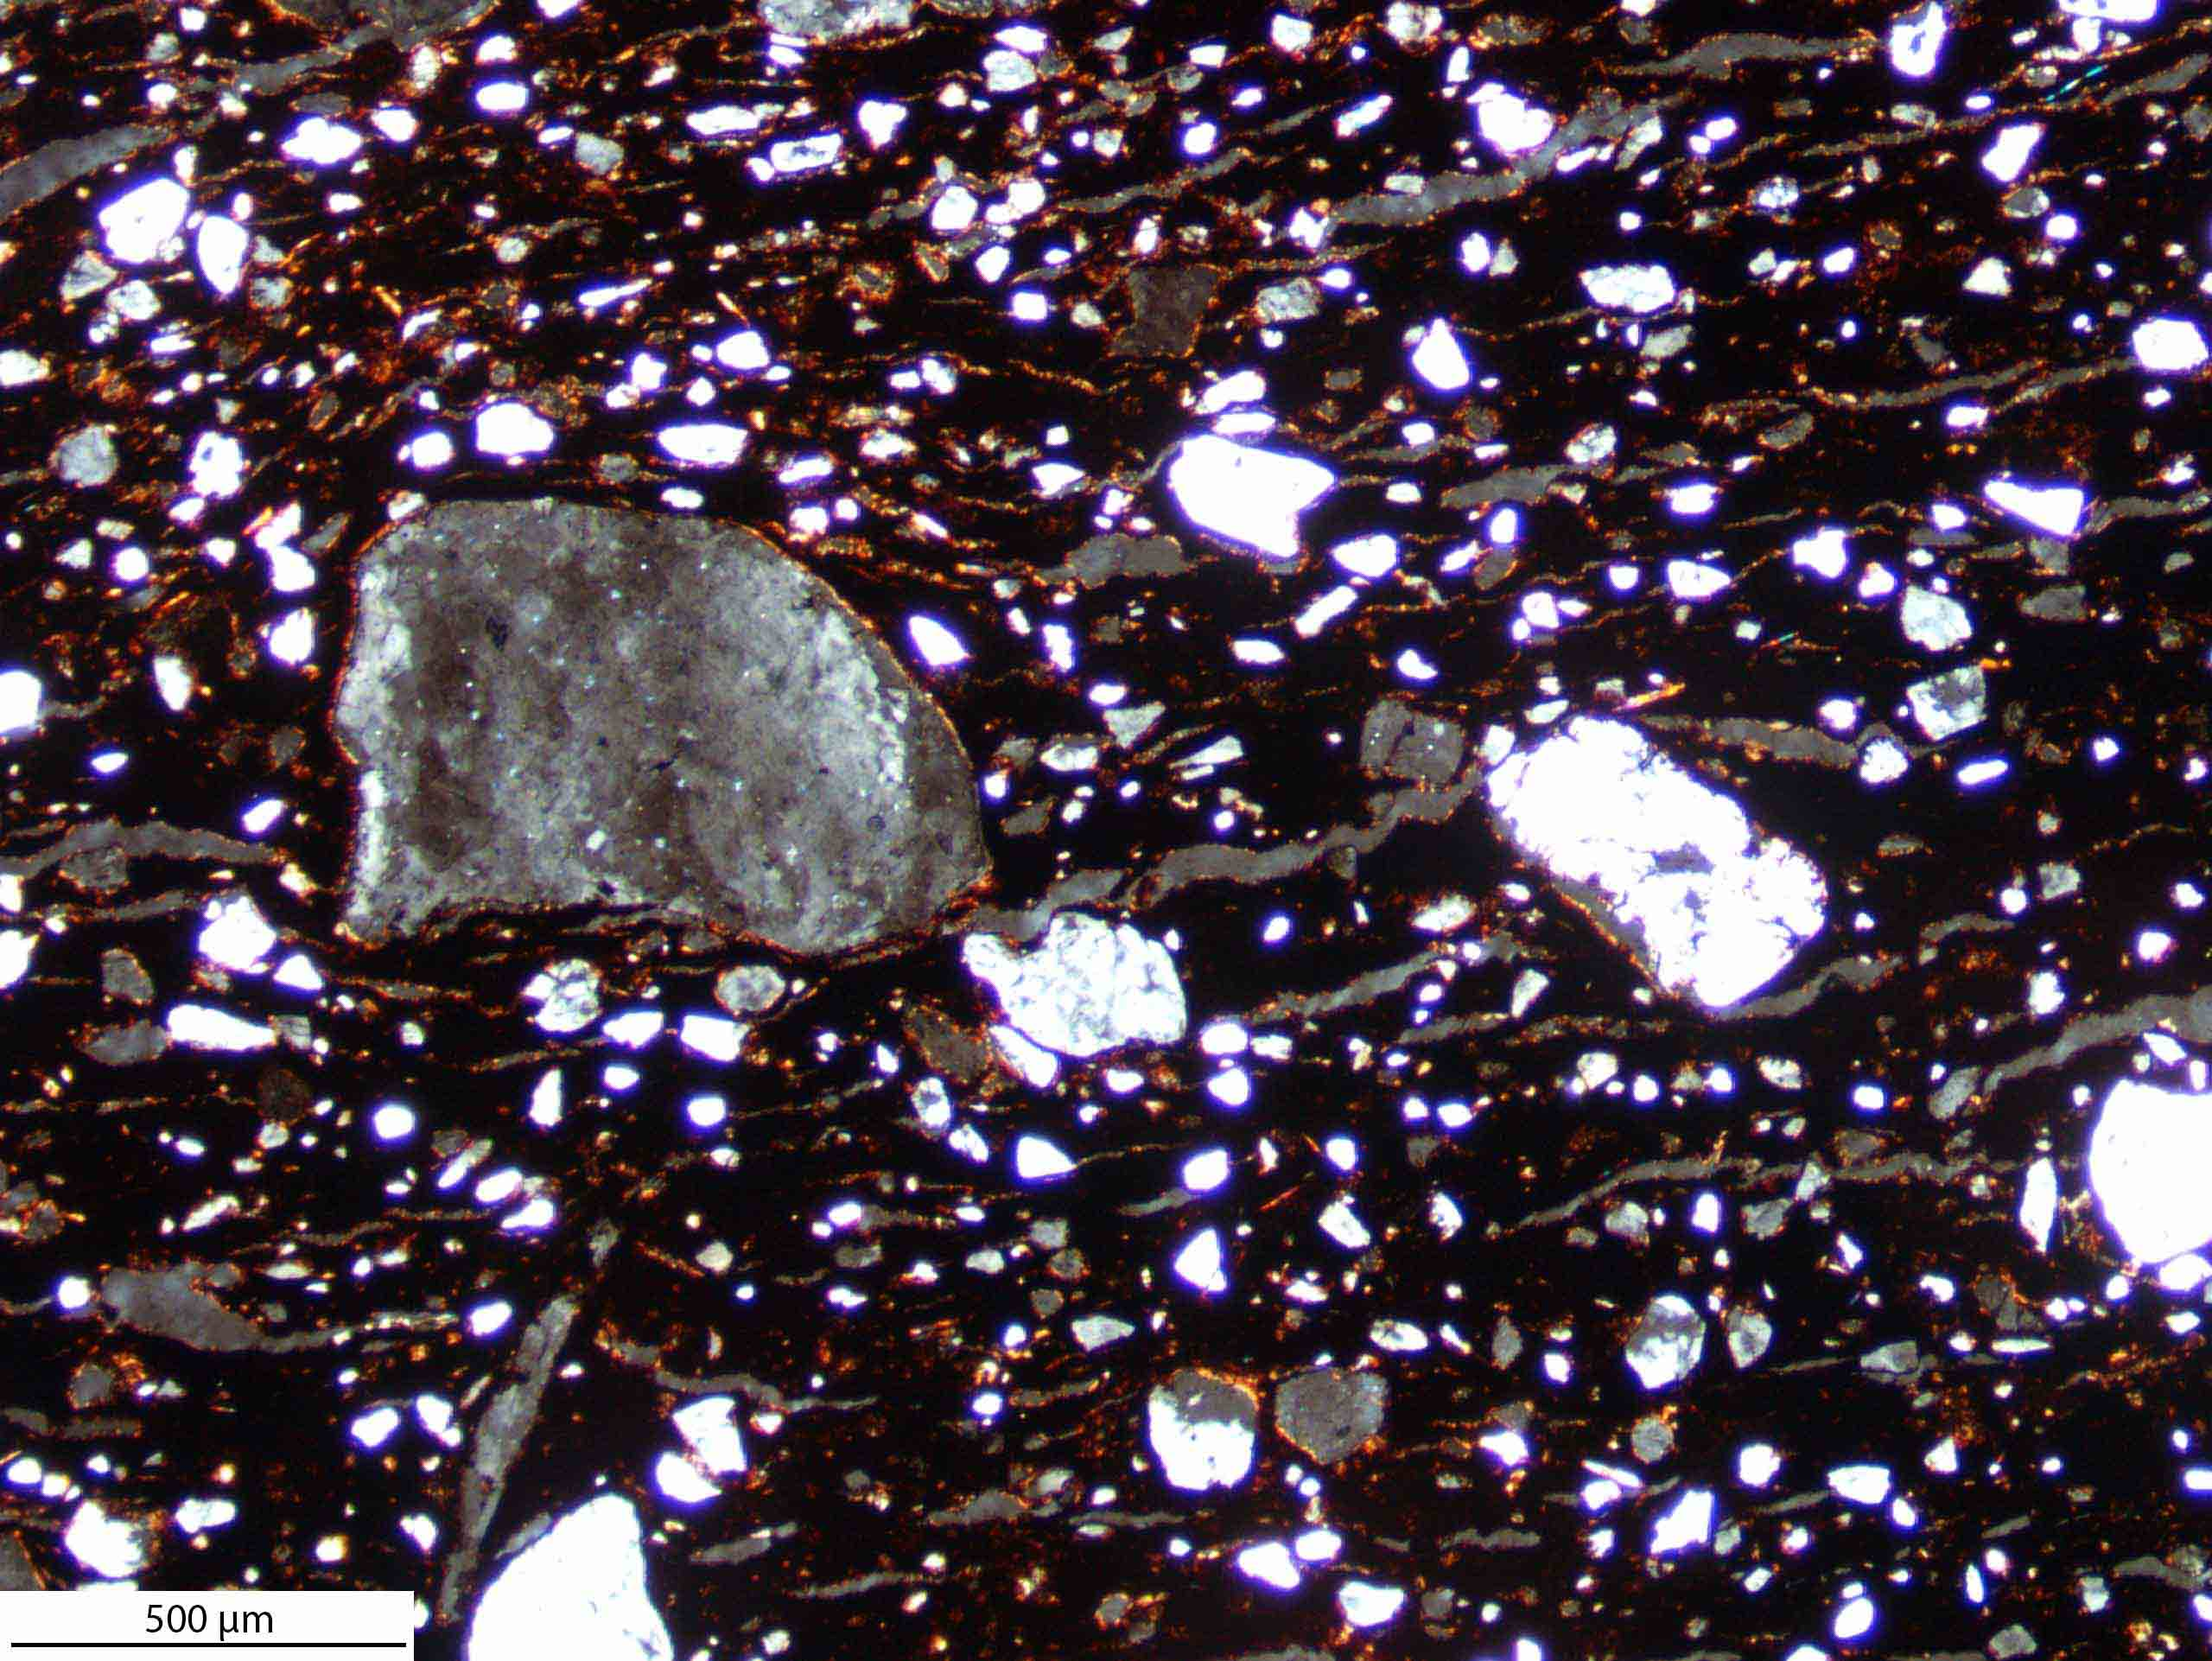
\includegraphics[width=\textwidth]{ThinSections/5-1_4x_XPL.jpg}
		\caption{[XPL]}
	\end{subfigure}
	\begin{subfigure}[t]{.49\textwidth}
		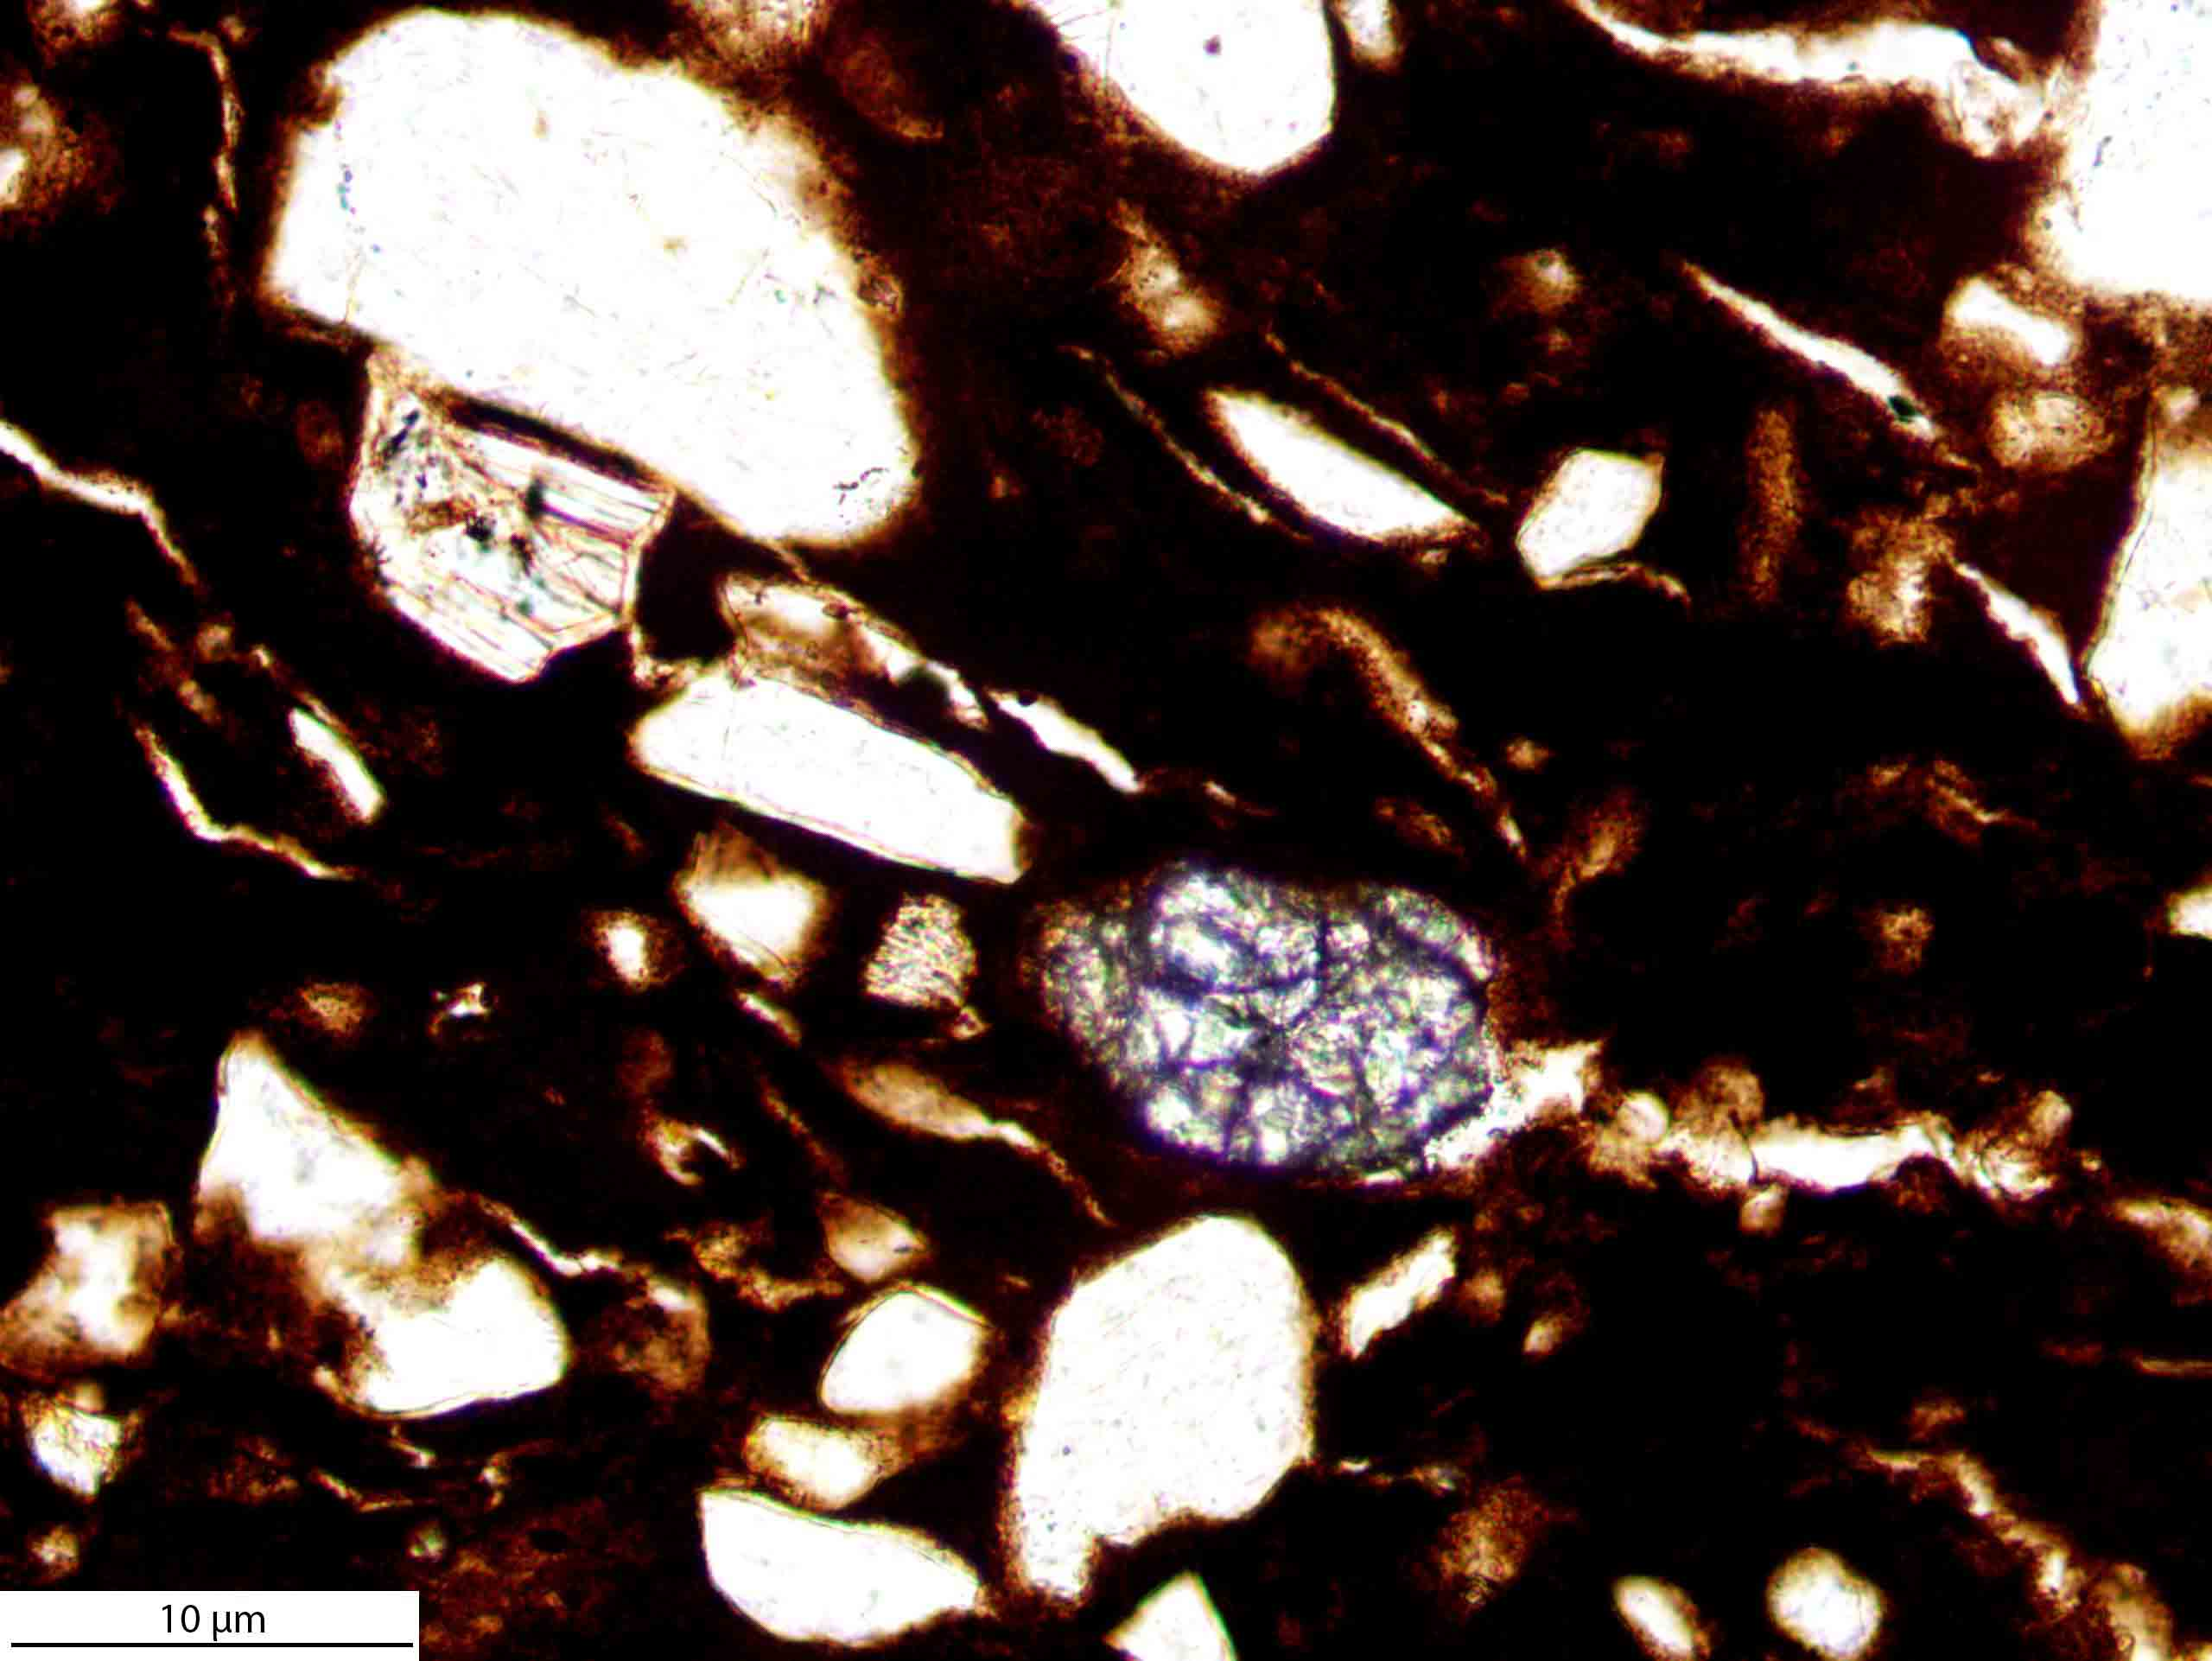
\includegraphics[width=\textwidth]{ThinSections/5-2_20x_PPL.jpg}
		\caption{Muscovite \& Zircon [PPL]}
	\end{subfigure}\hspace{.5em}\hfill
	\begin{subfigure}[t]{.49\textwidth}
		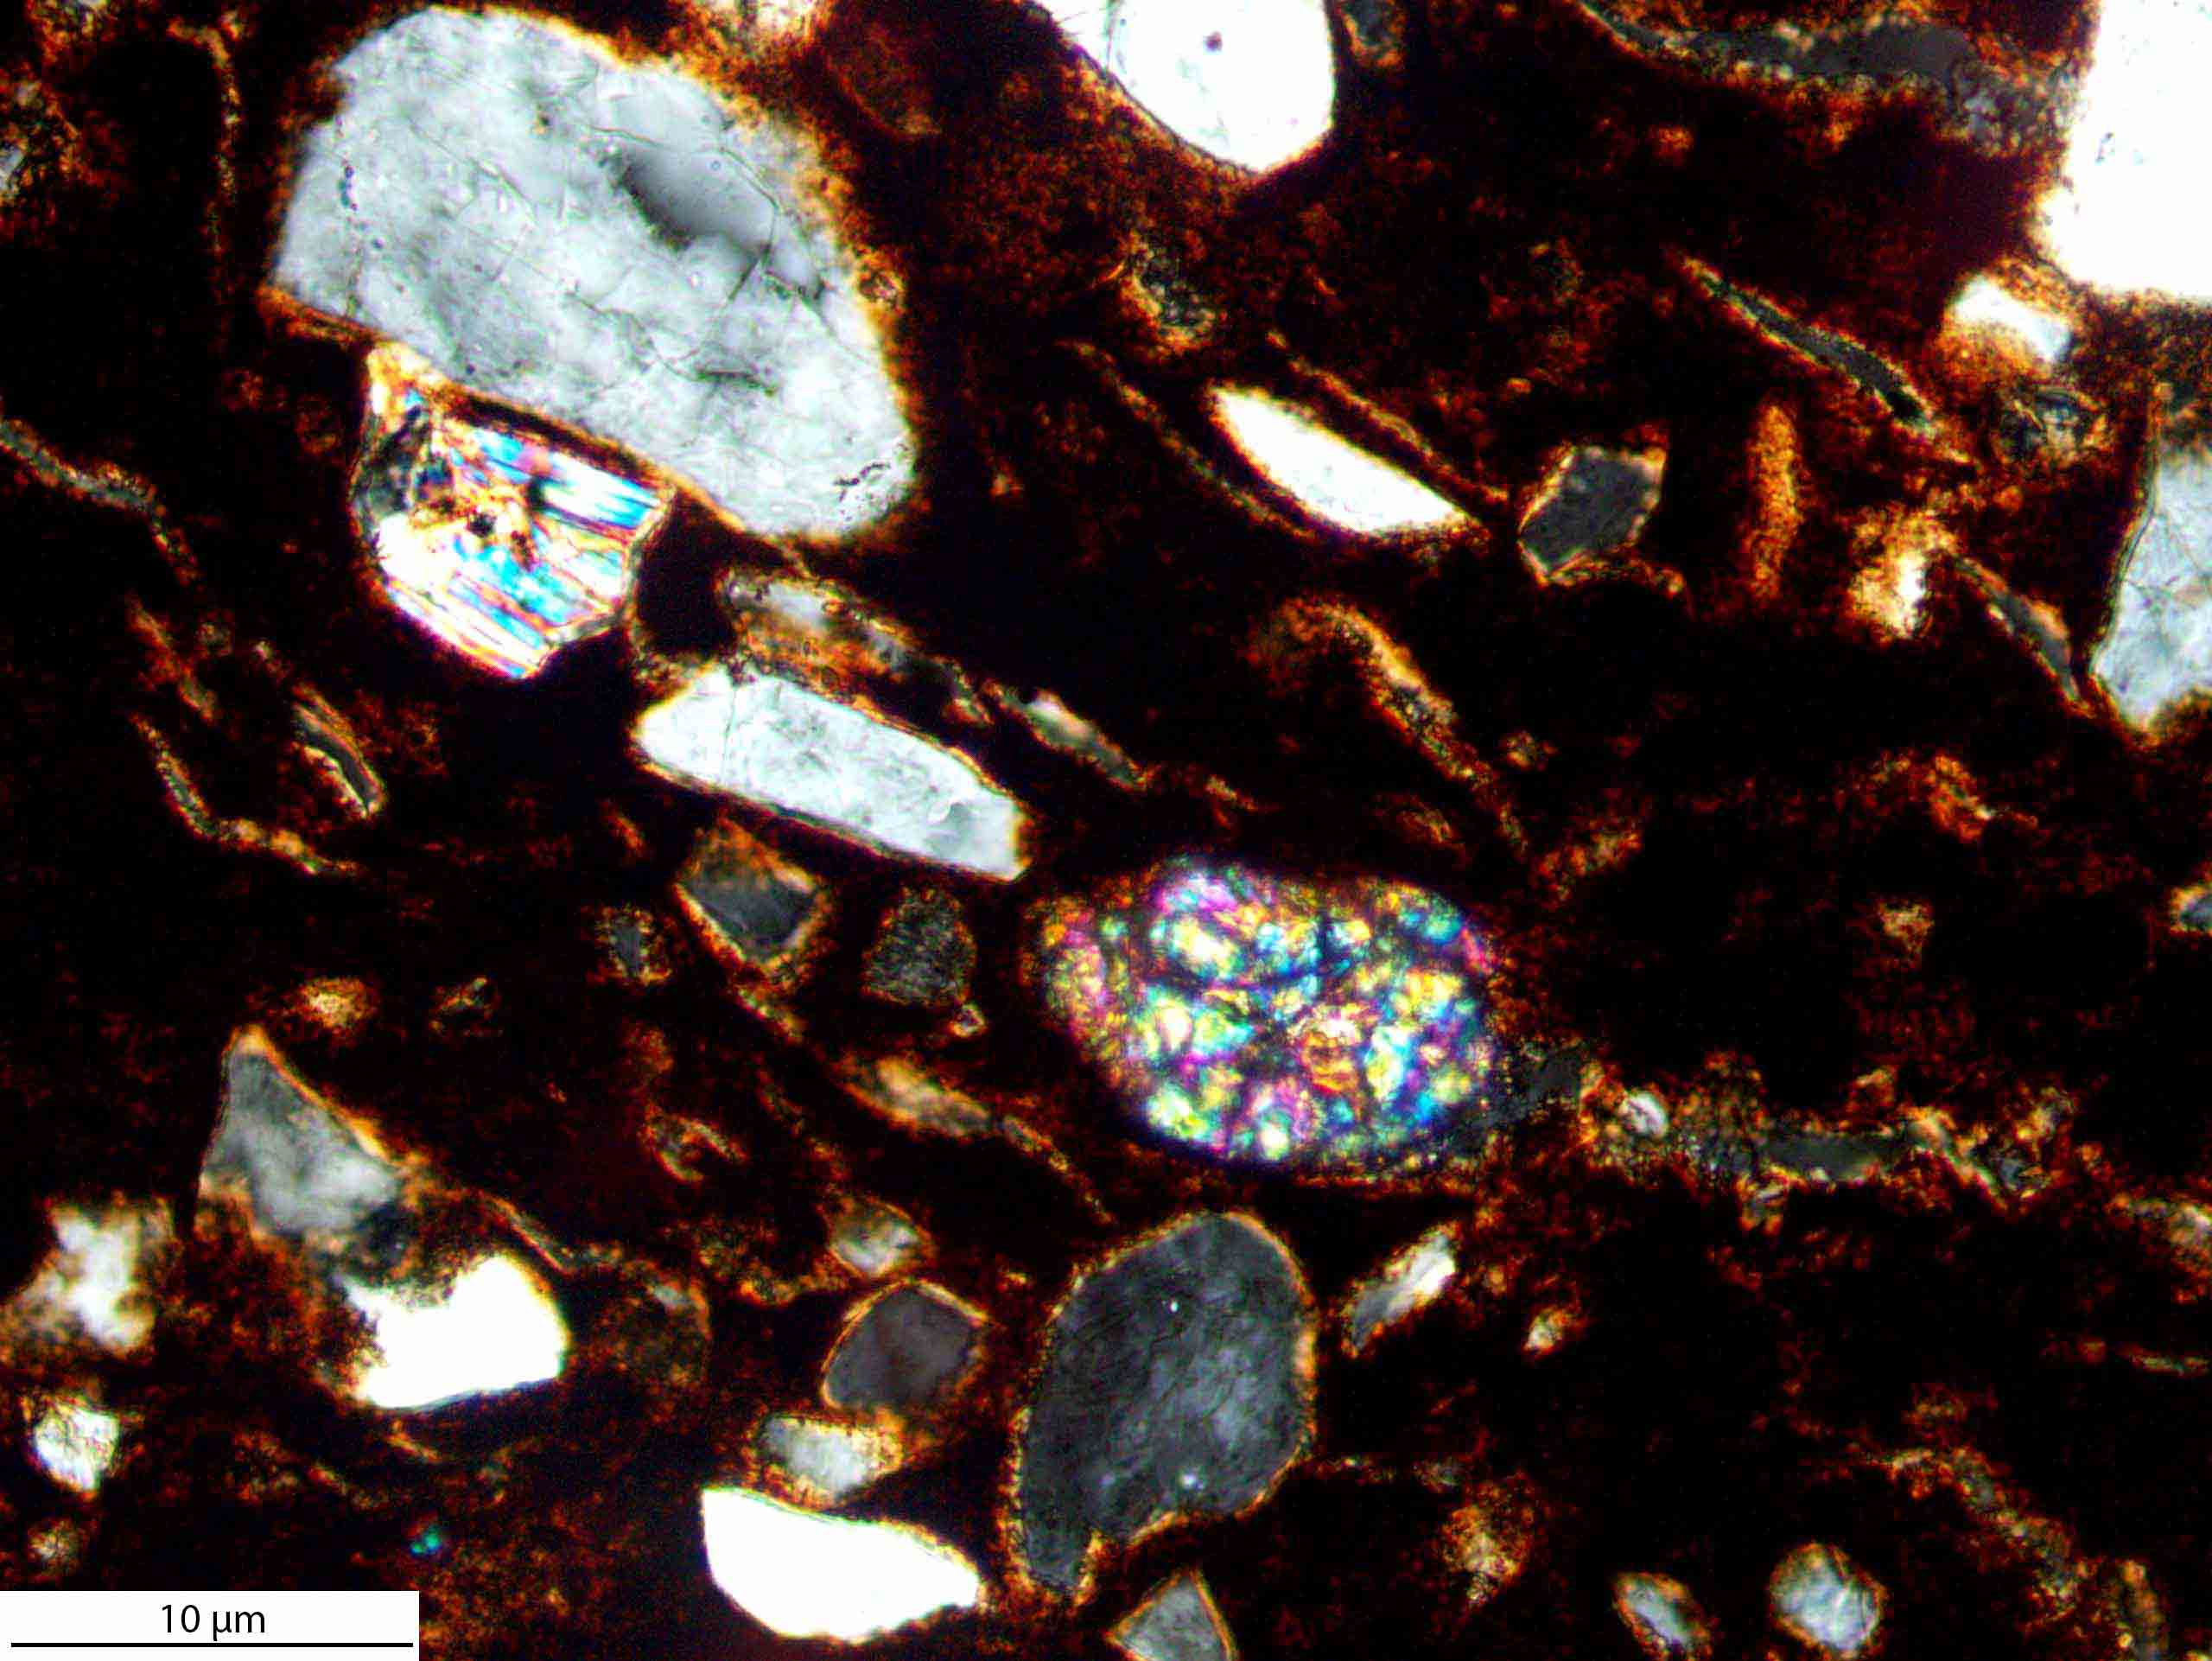
\includegraphics[width=\textwidth]{ThinSections/5-2_20x_XPL.jpg}
		\caption{Muscovite \& Zircon [XPL]}
	\end{subfigure}
	\caption{}
	\label{fig:5_pik}
\end{figure}

\newpage\subsection{PIK~87/1-8:2 \citep[pik\#56; Fig.~\ref{fig:pik.pottery}.7; cf. Ngbanja style;][428 Pl.~47.21]{Seidensticker.2021e}}

\begin{multicols}{2}
\noindent The fine fraction is homogeneous, non-calcareous, and slightly iron rich (reddish-brown [PPL]) with undifferentiated to slighly stipple-speckled b-farbic. Voids are very narrow and oriented diagonally in relation to the plane of the section; similar as the coarse fraction. The dominant component of the coarse-fractions is densely packed, unimodally sorted, angular to sub-angular quartz. Some quartz grains shows rolling extinction (b), indicating metamorphic degradation. Some of the larger constituents of the coarse fraction are rock fragments (sandstone) (c--d). Occasionally present are muscovite,  biotite, tourmaline, staurolite, and zircon. The c/f-related distribution pattern is single-spaced porphyric.
\end{multicols}

% tourmaline
% also present: muscovite, monazite(?), ??

%\vfill
\begin{figure}[H]
	\centering
	\begin{subfigure}[t]{.49\textwidth}
		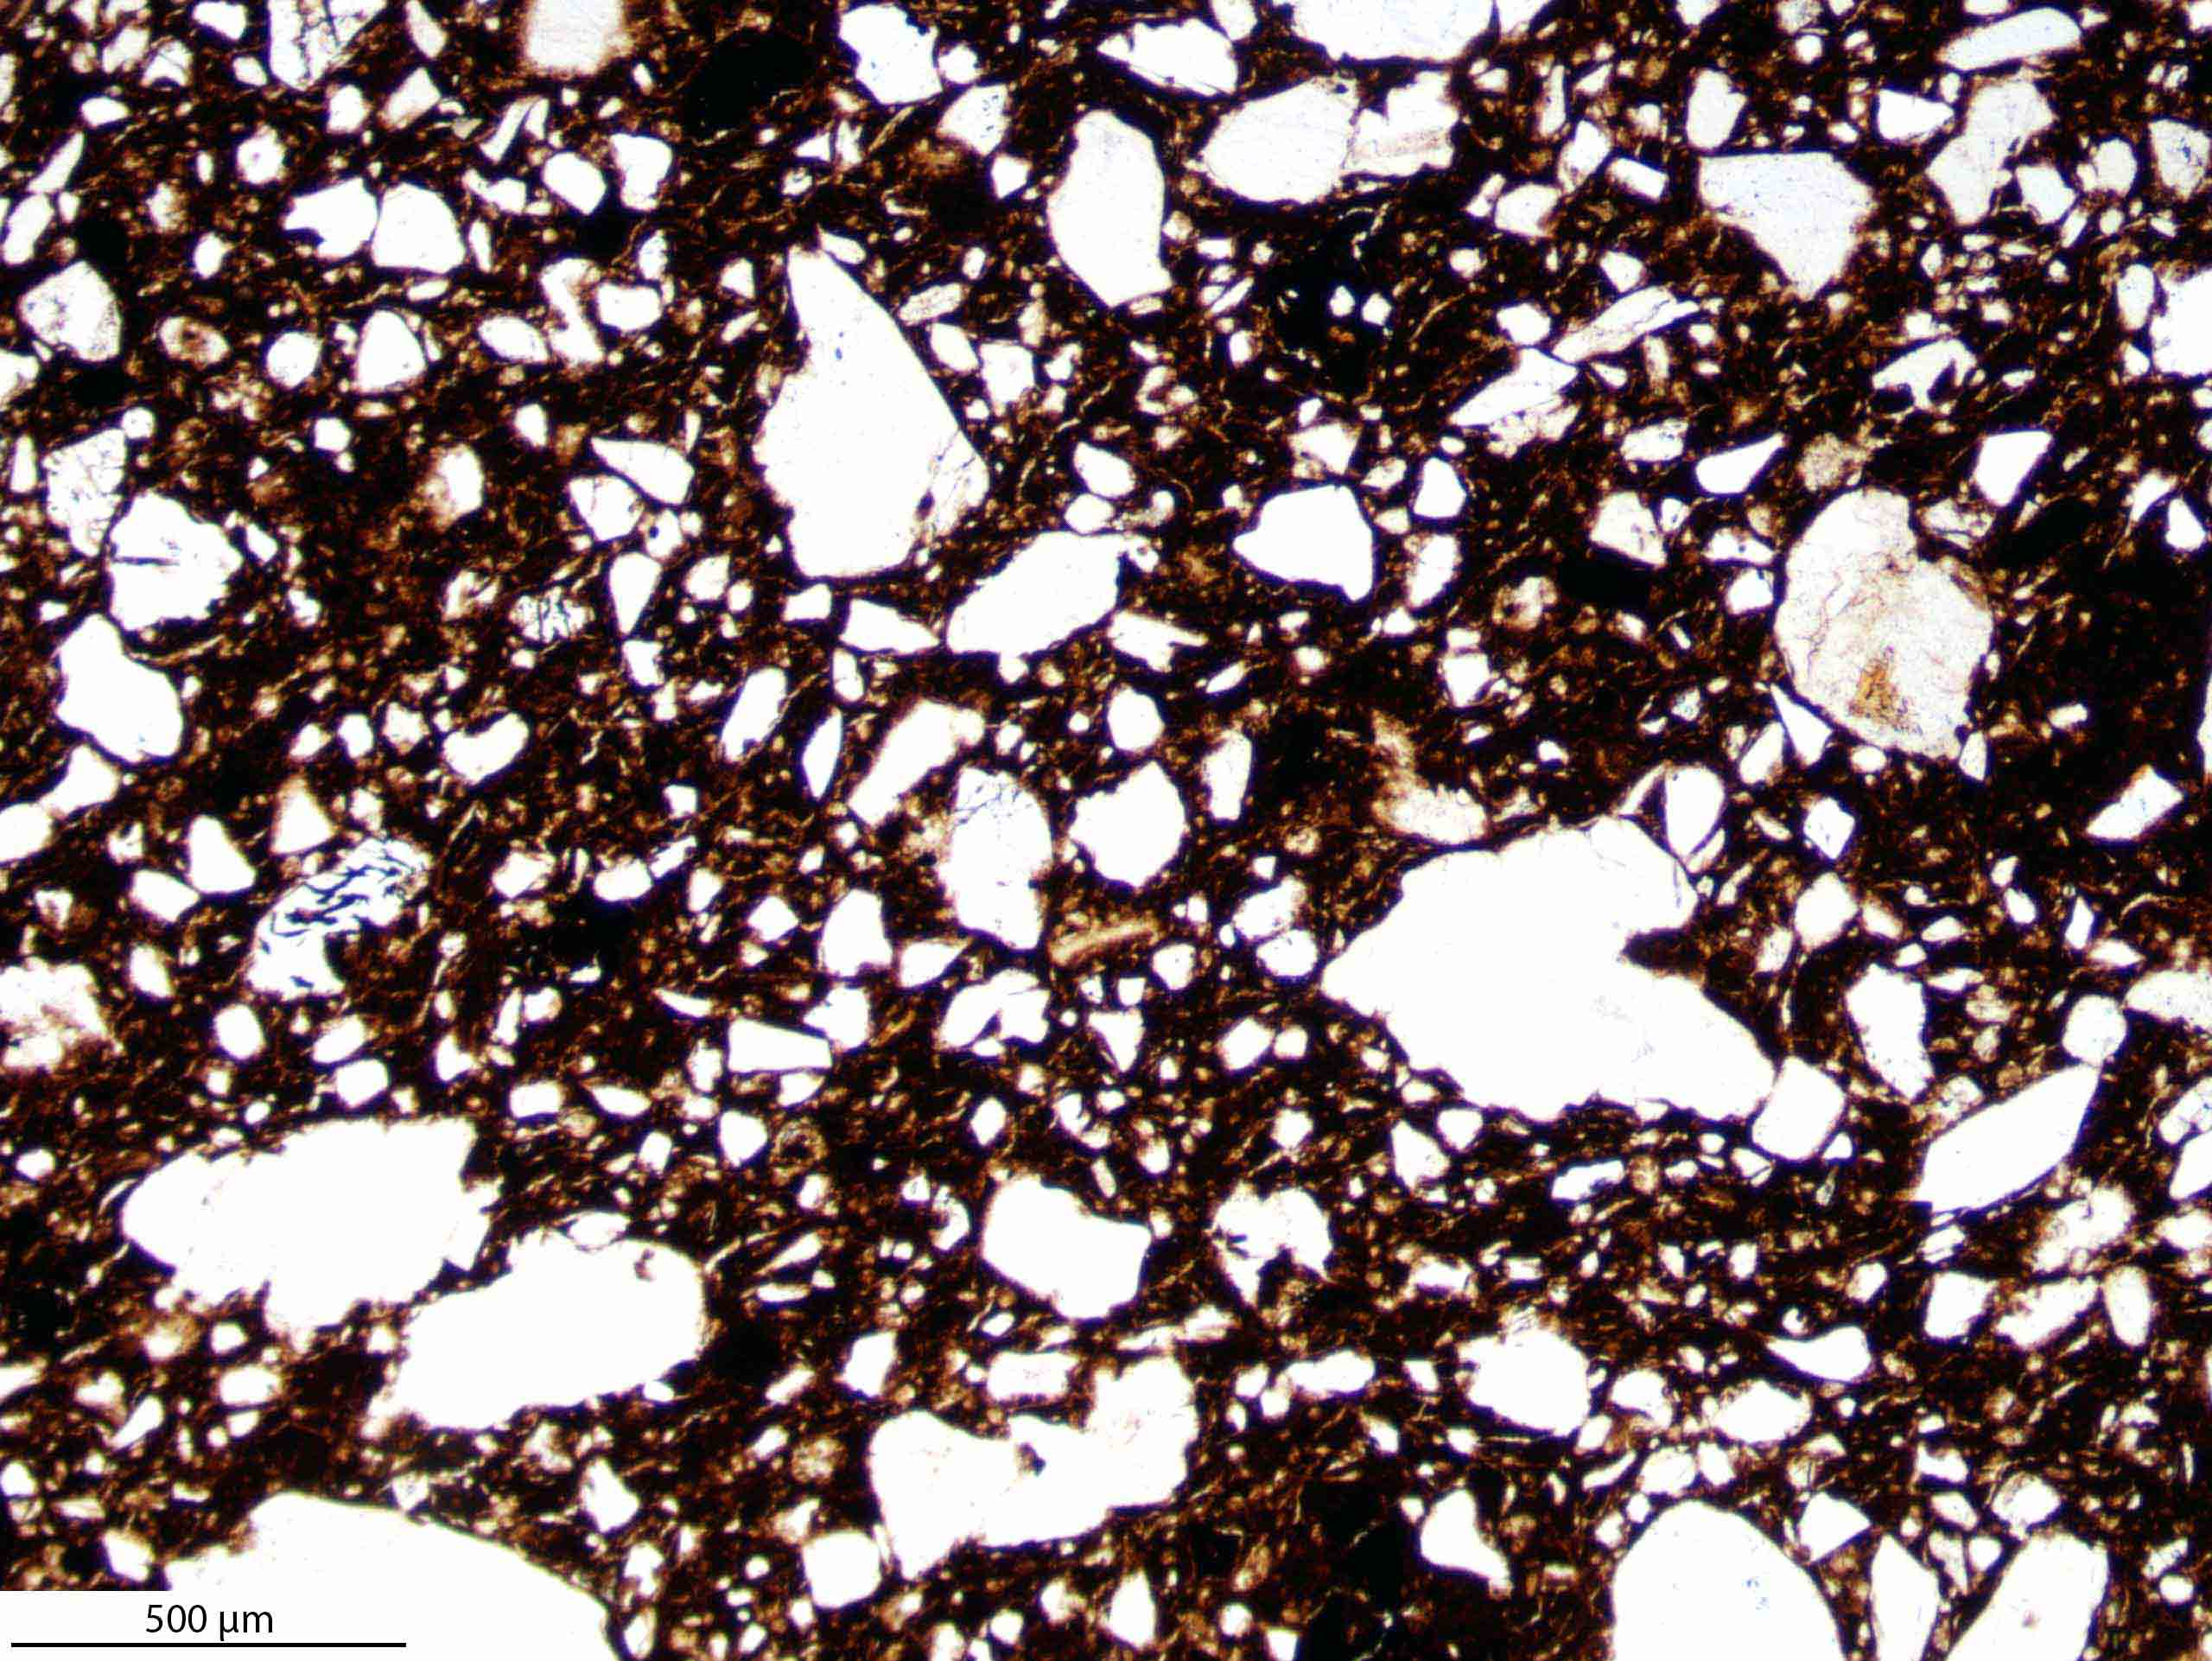
\includegraphics[width=\textwidth]{ThinSections/56-1_4x_PPL.jpg}
		\caption{[PPL]}
	\end{subfigure}\hspace{.5em}\hfill
	\begin{subfigure}[t]{.49\textwidth}
		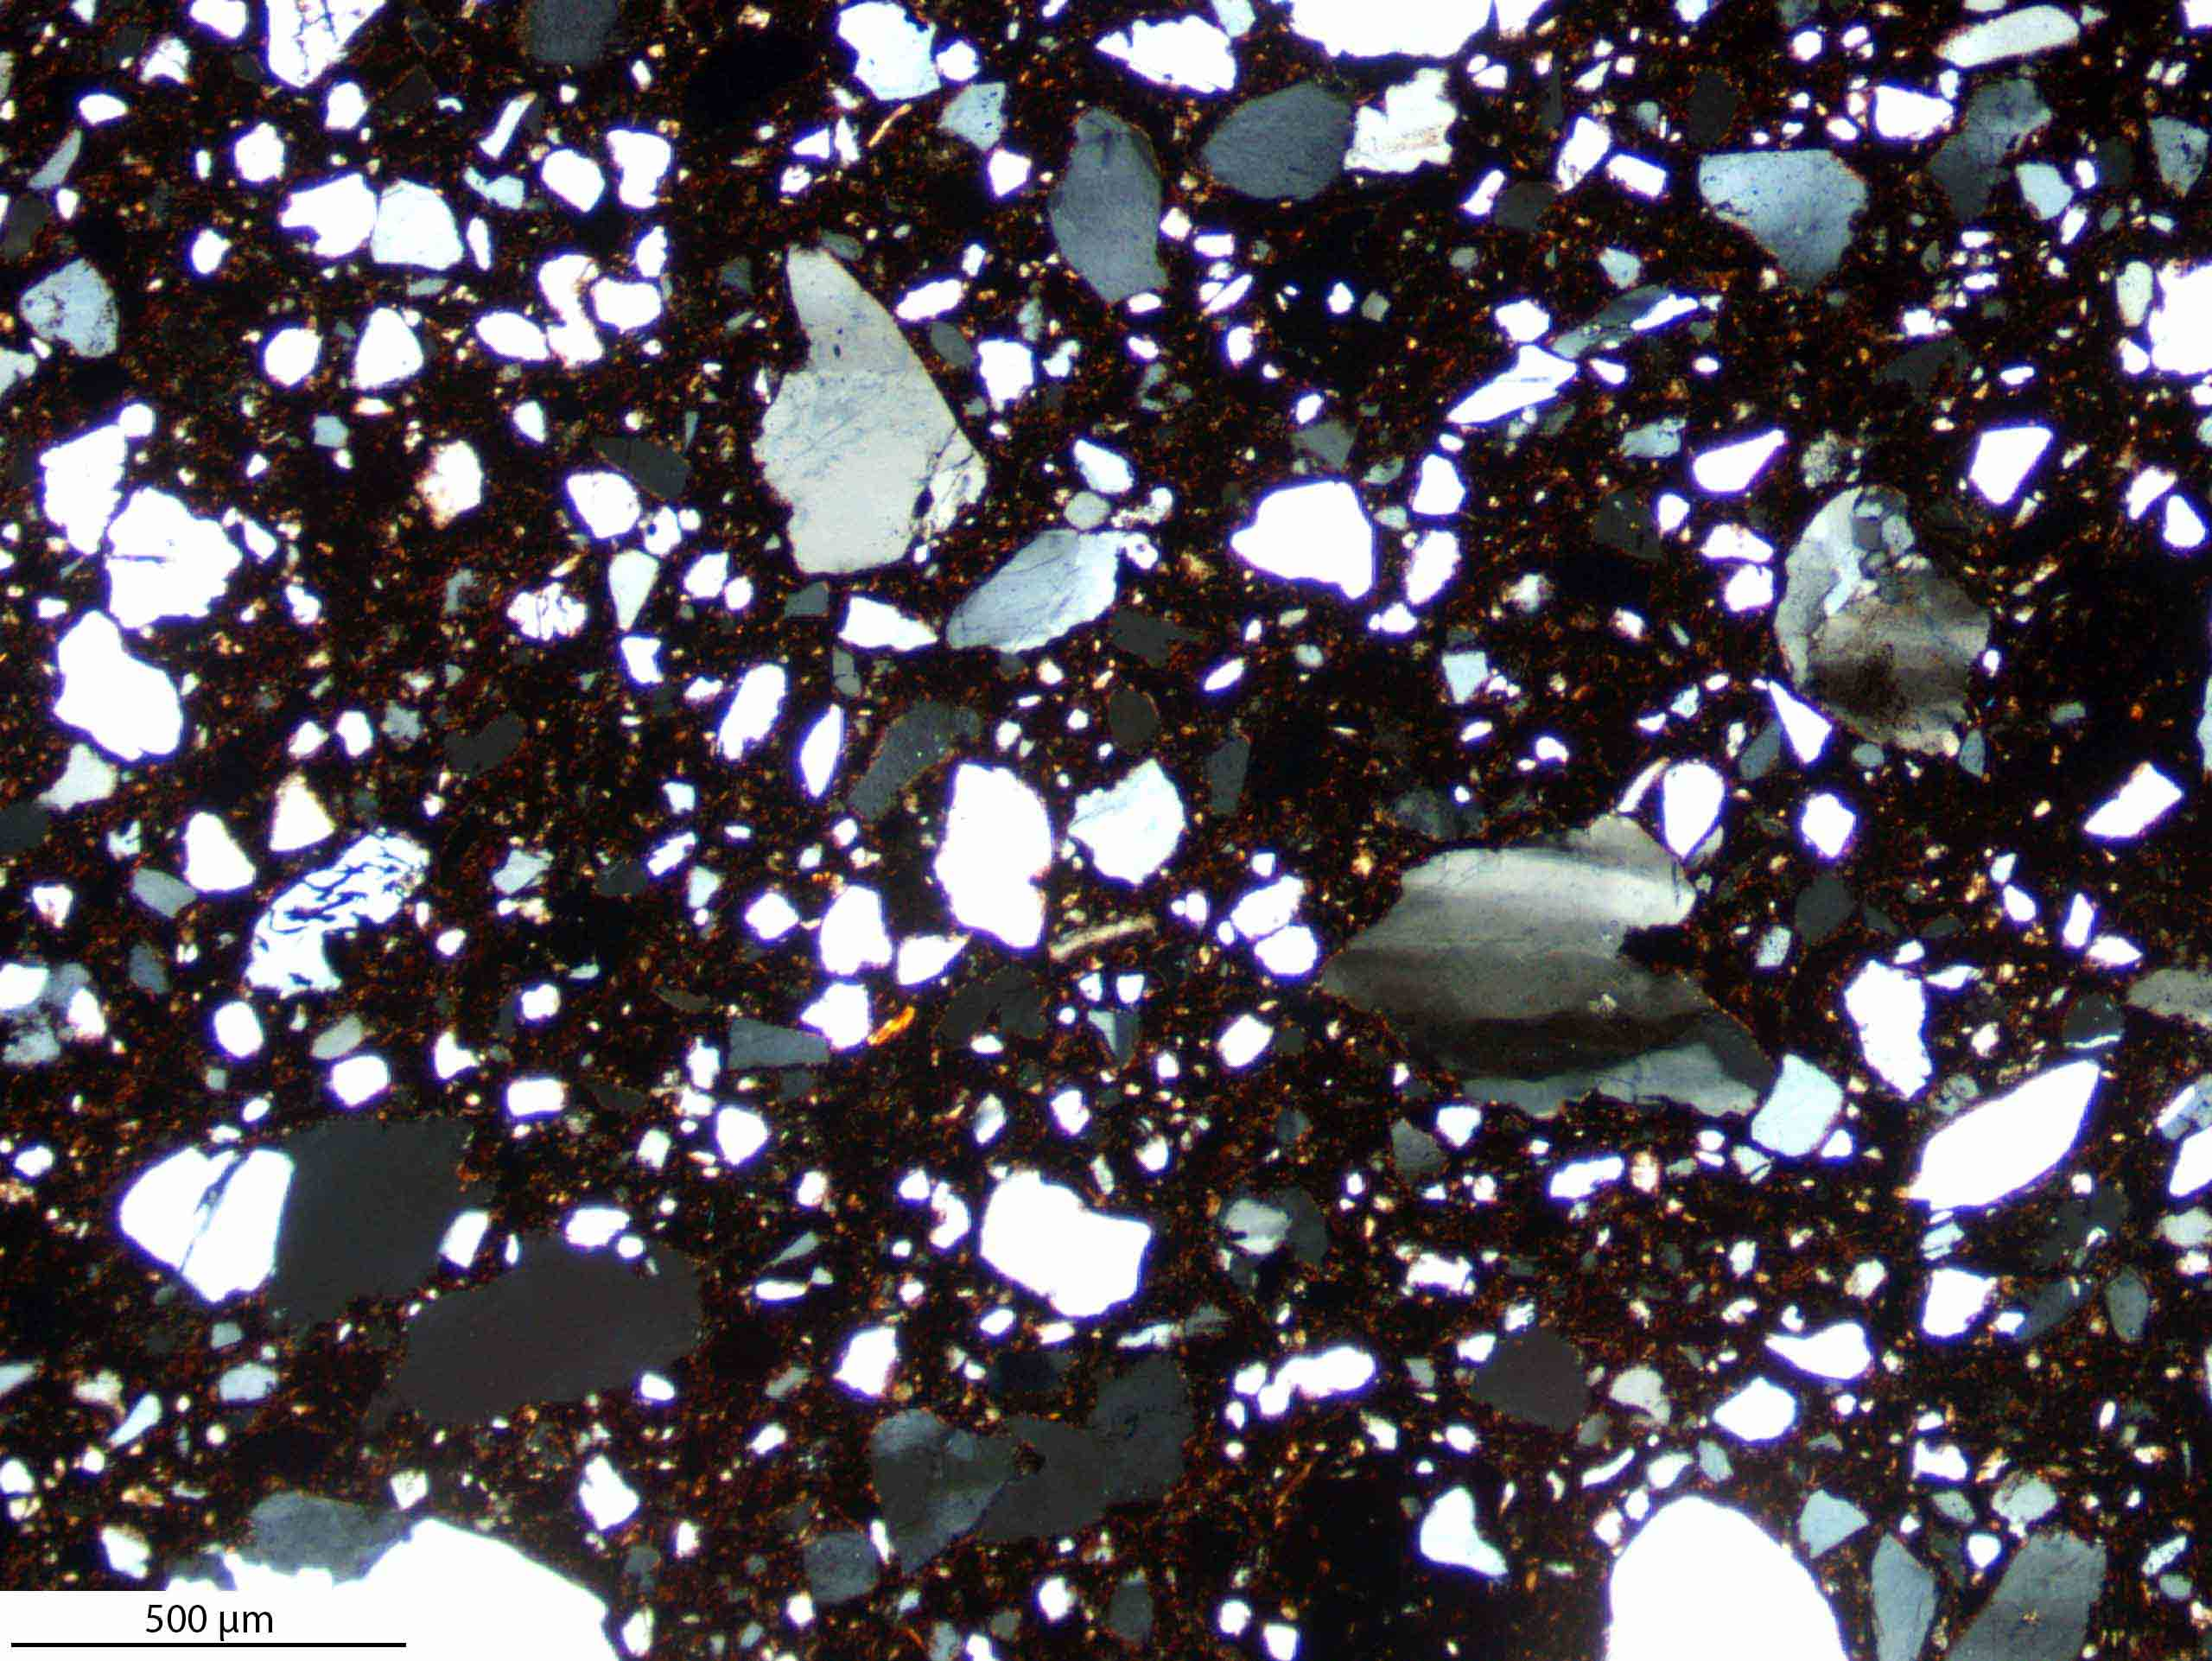
\includegraphics[width=\textwidth]{ThinSections/56-1_4x_XPL.jpg}
		\caption{[XPL]}
	\end{subfigure}
	\begin{subfigure}[t]{.49\textwidth}
		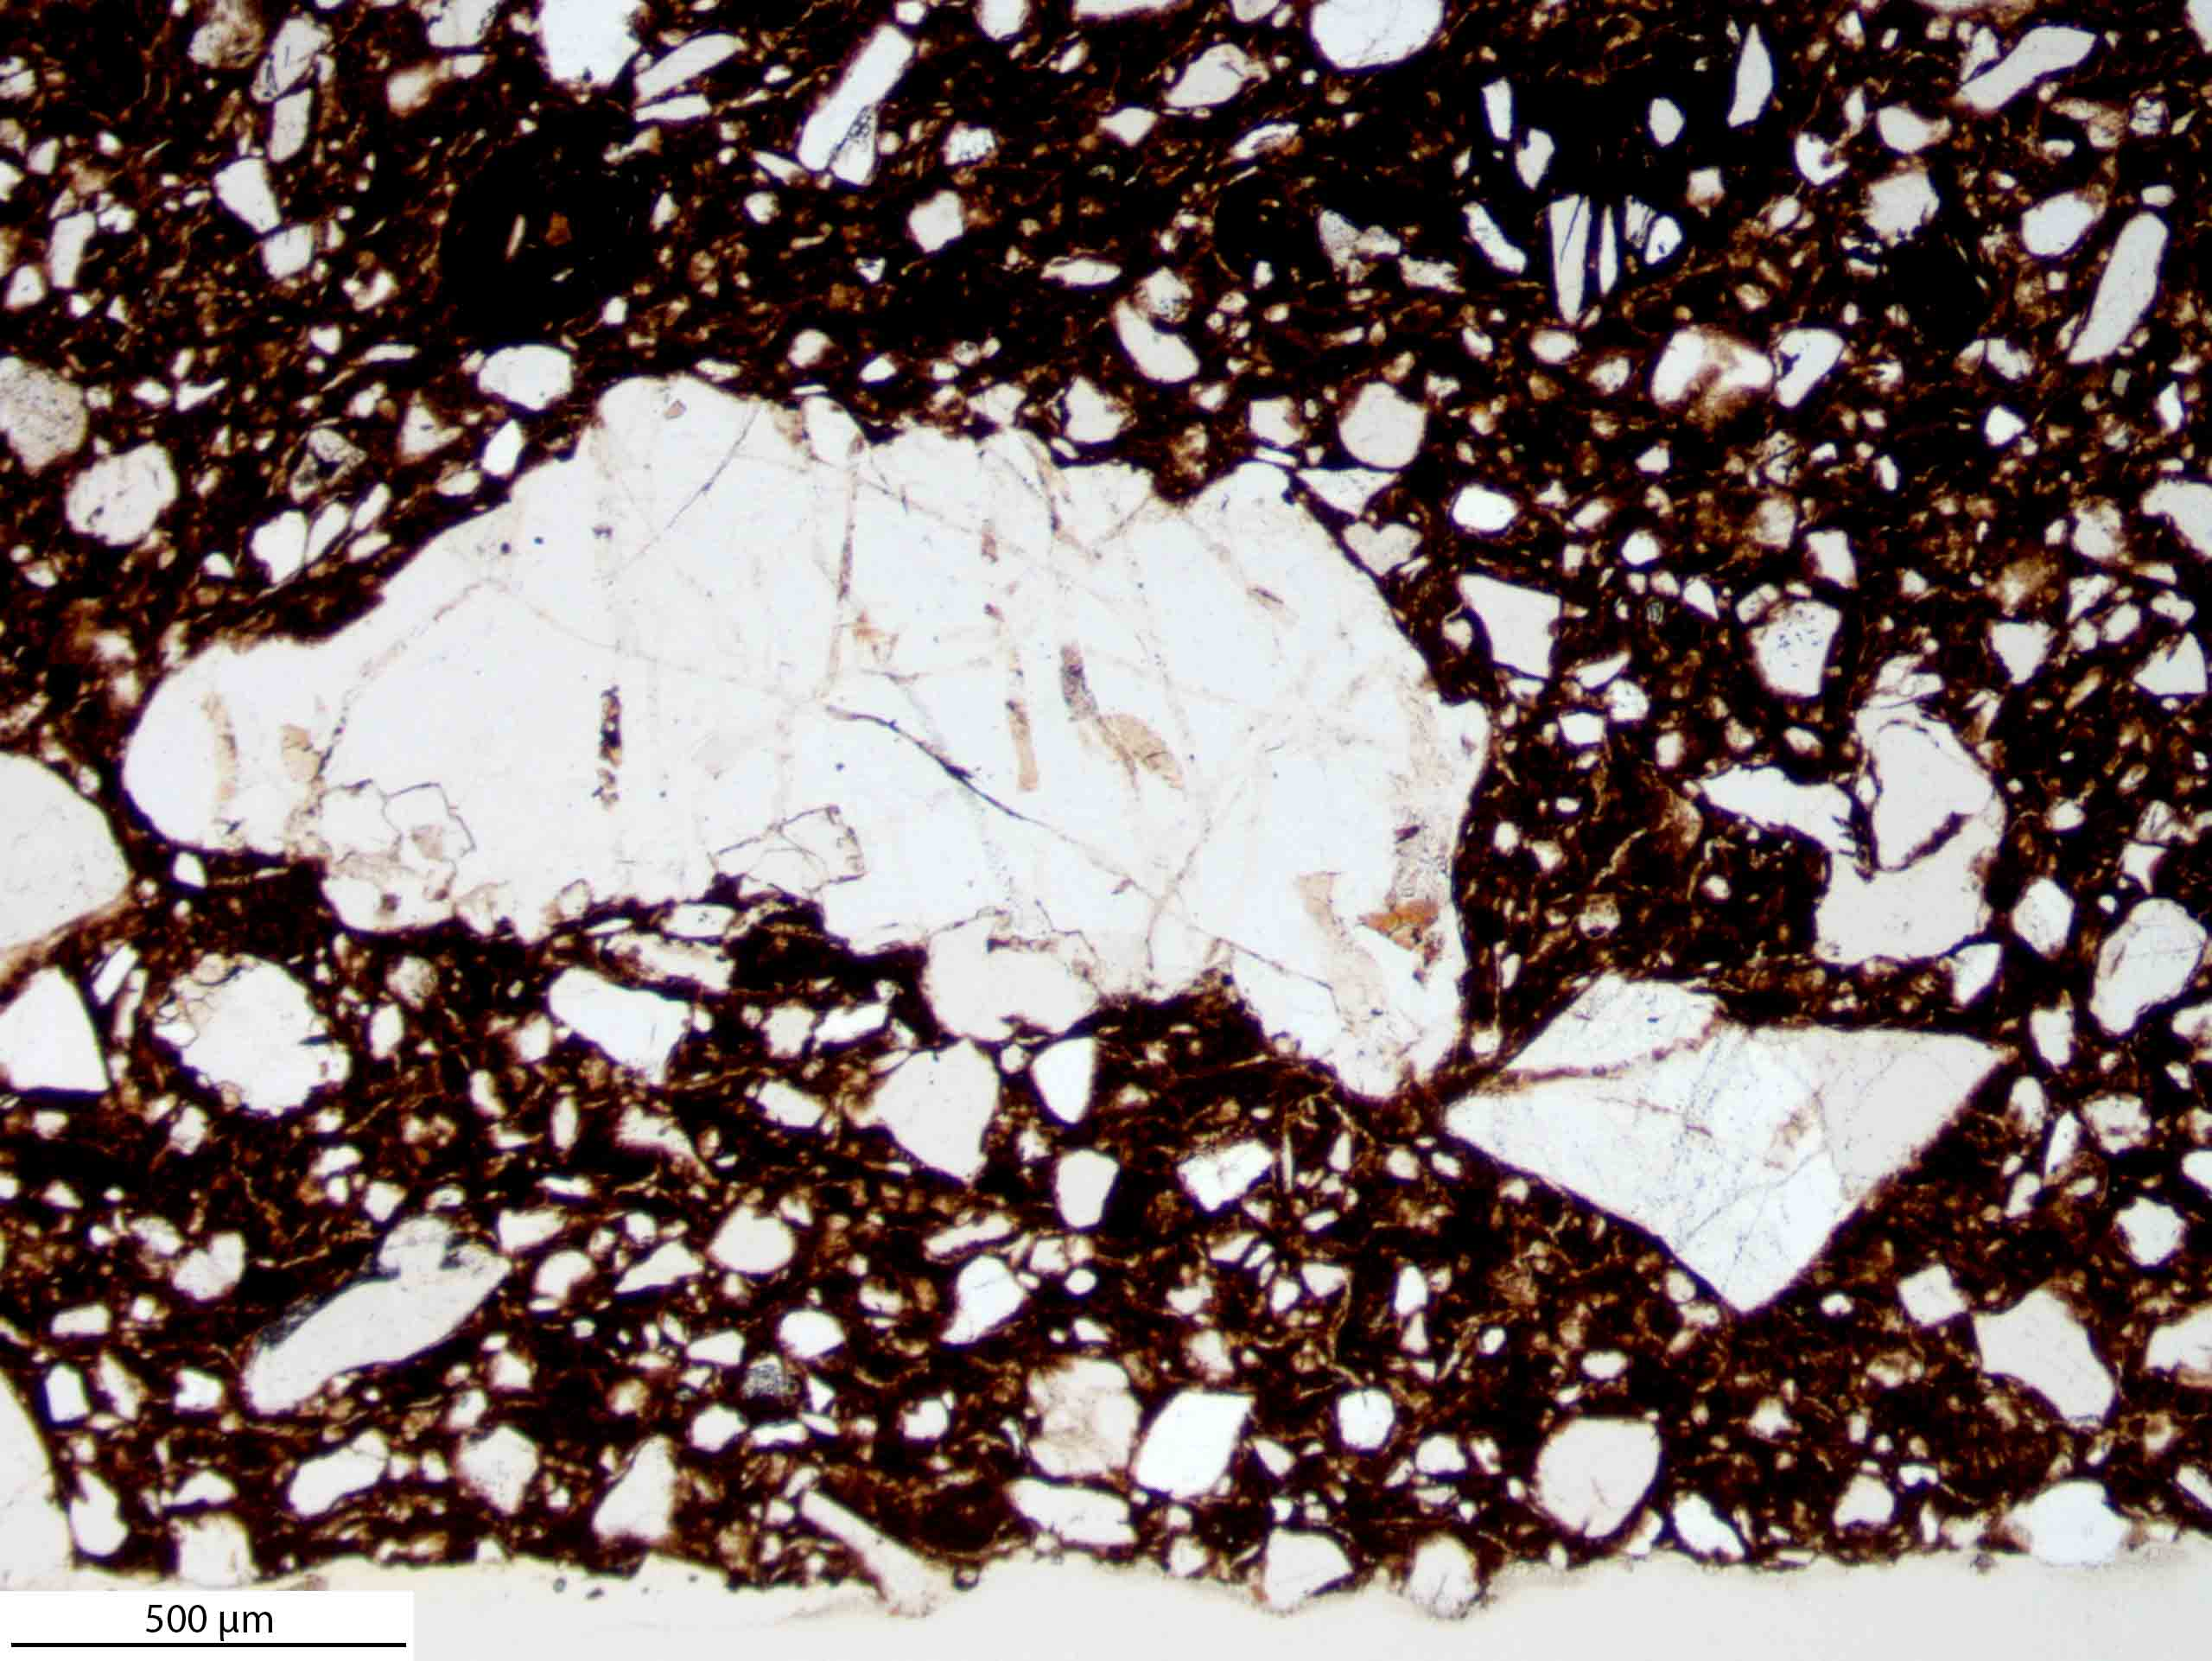
\includegraphics[width=\textwidth]{ThinSections/56-2_4x_PPL.jpg}
		\caption{Rock fragment [PPL]}
	\end{subfigure}\hspace{.5em}\hfill
	\begin{subfigure}[t]{.49\textwidth}
		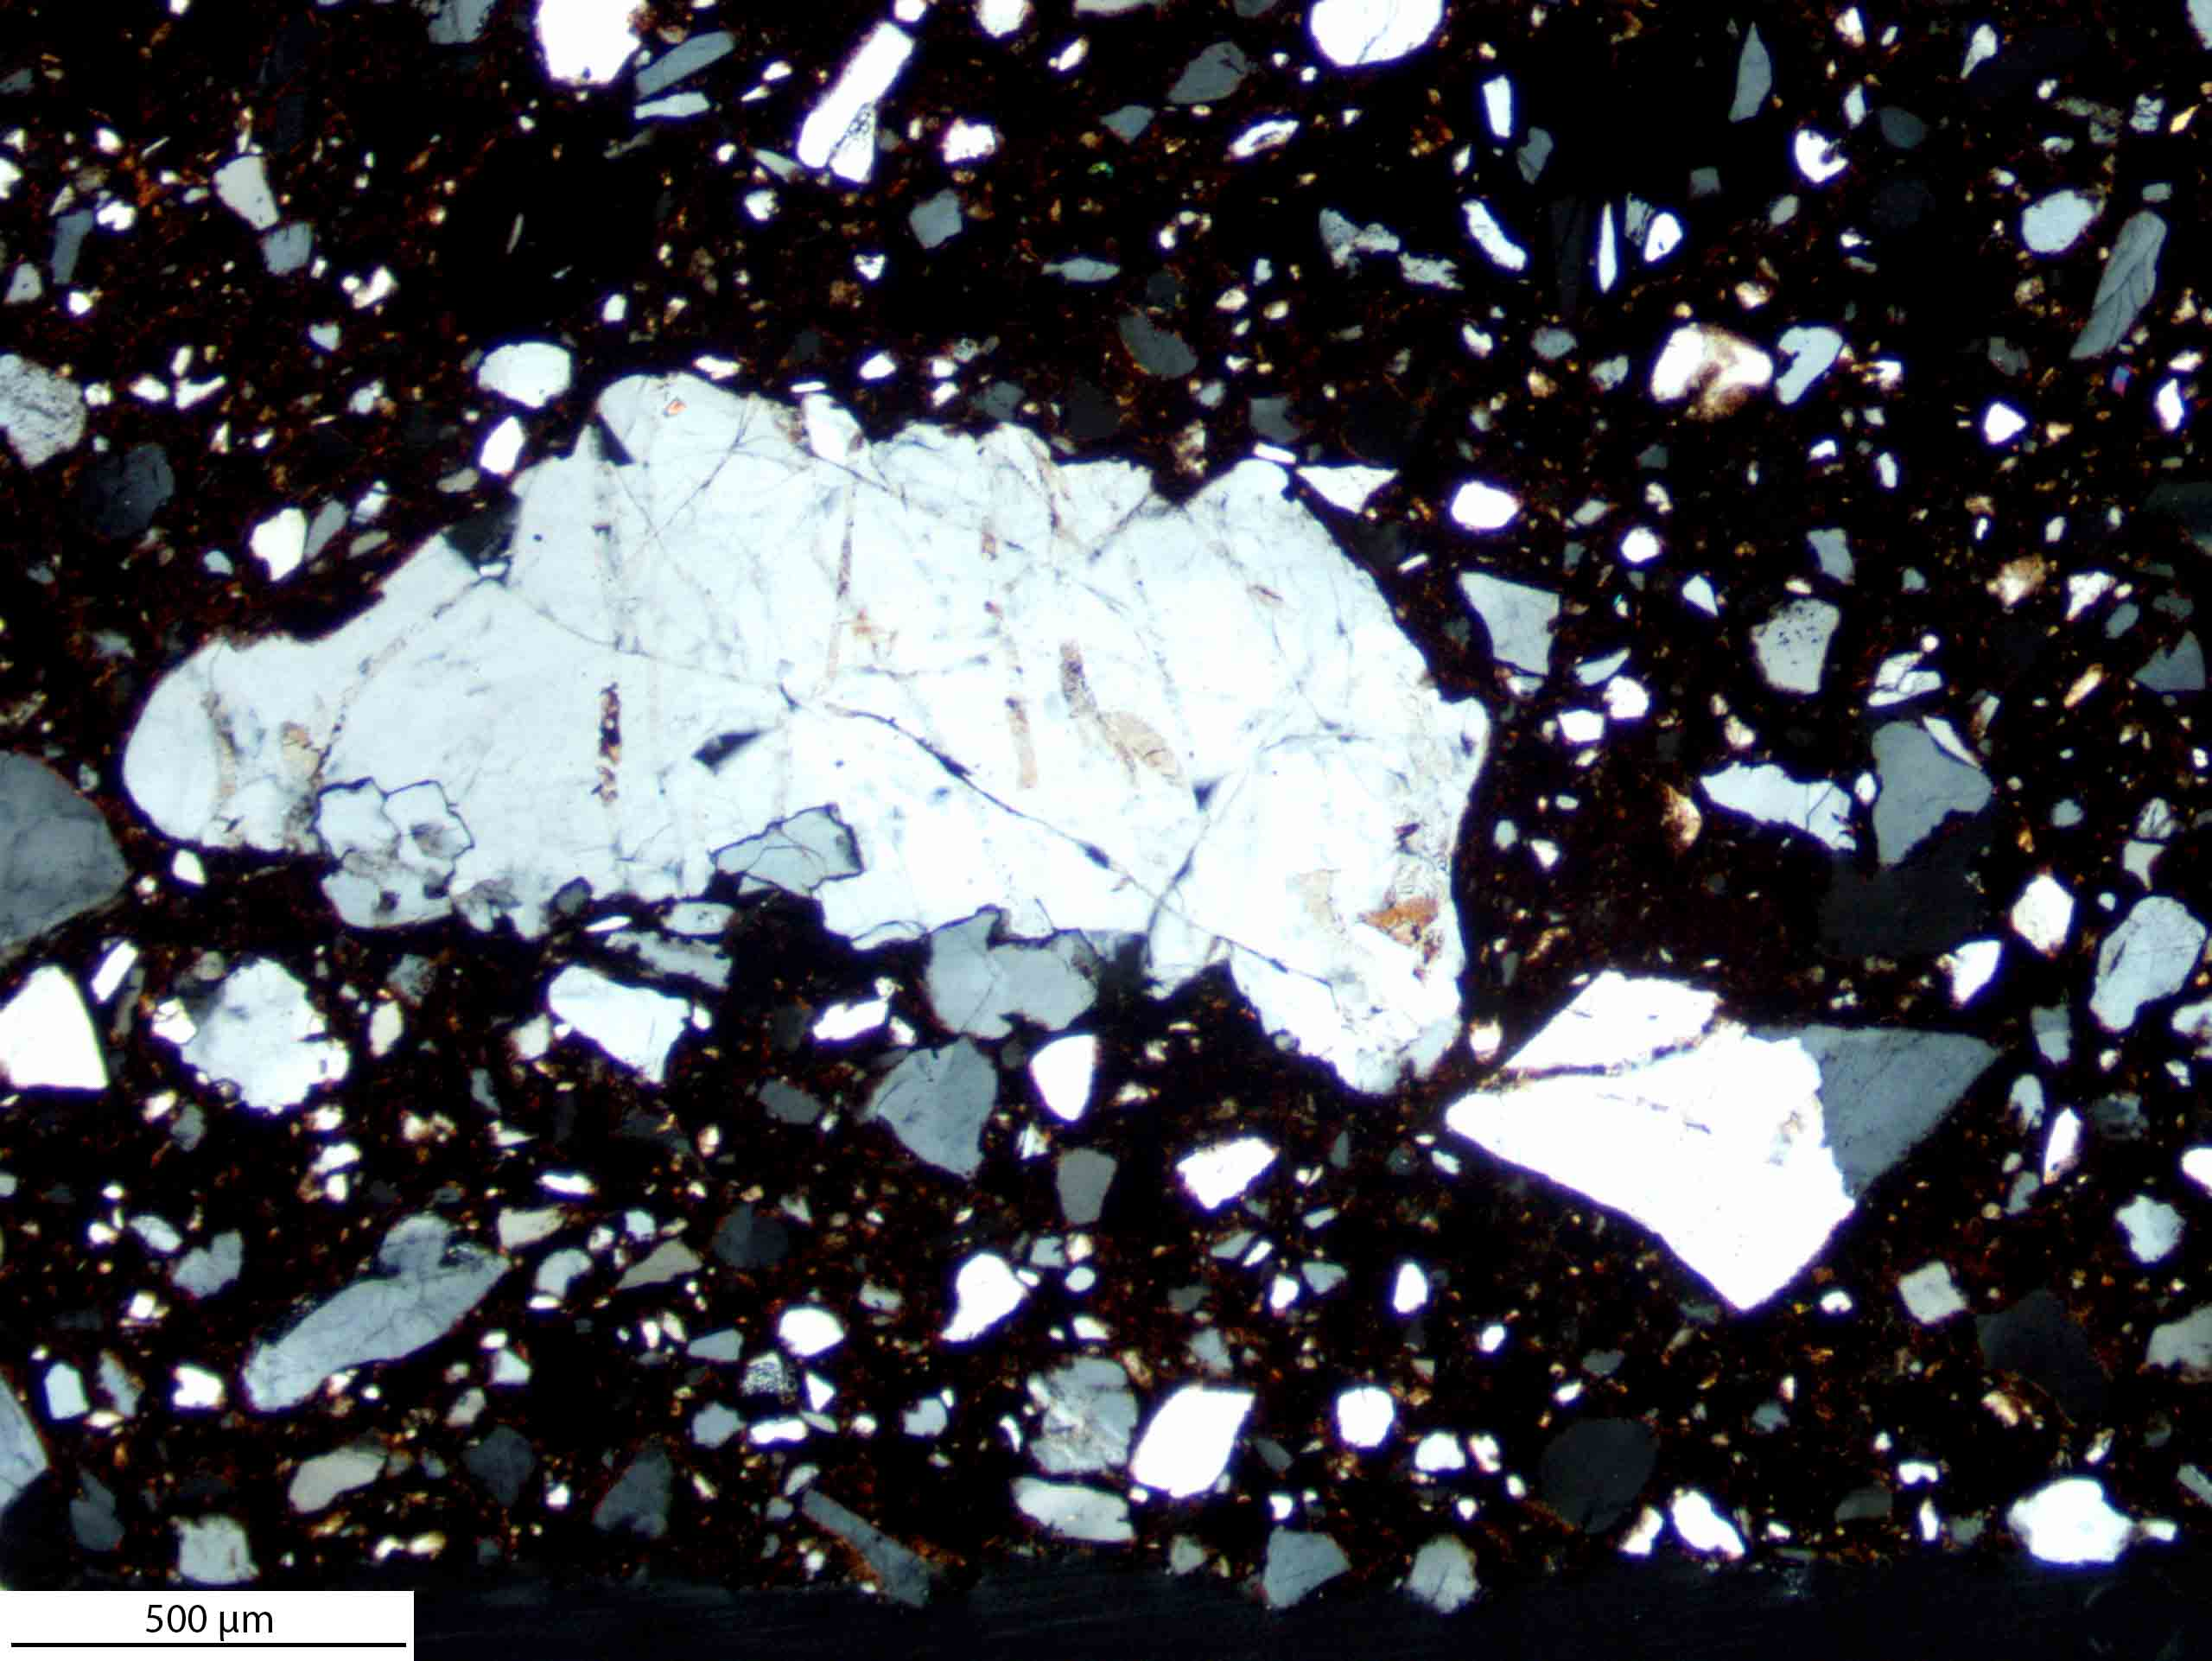
\includegraphics[width=\textwidth]{ThinSections/56-2_4x_XPL.jpg}
		\caption{Rock fragment [XPL]}
	\end{subfigure}
%	\begin{subfigure}[t]{.24\textwidth}
%		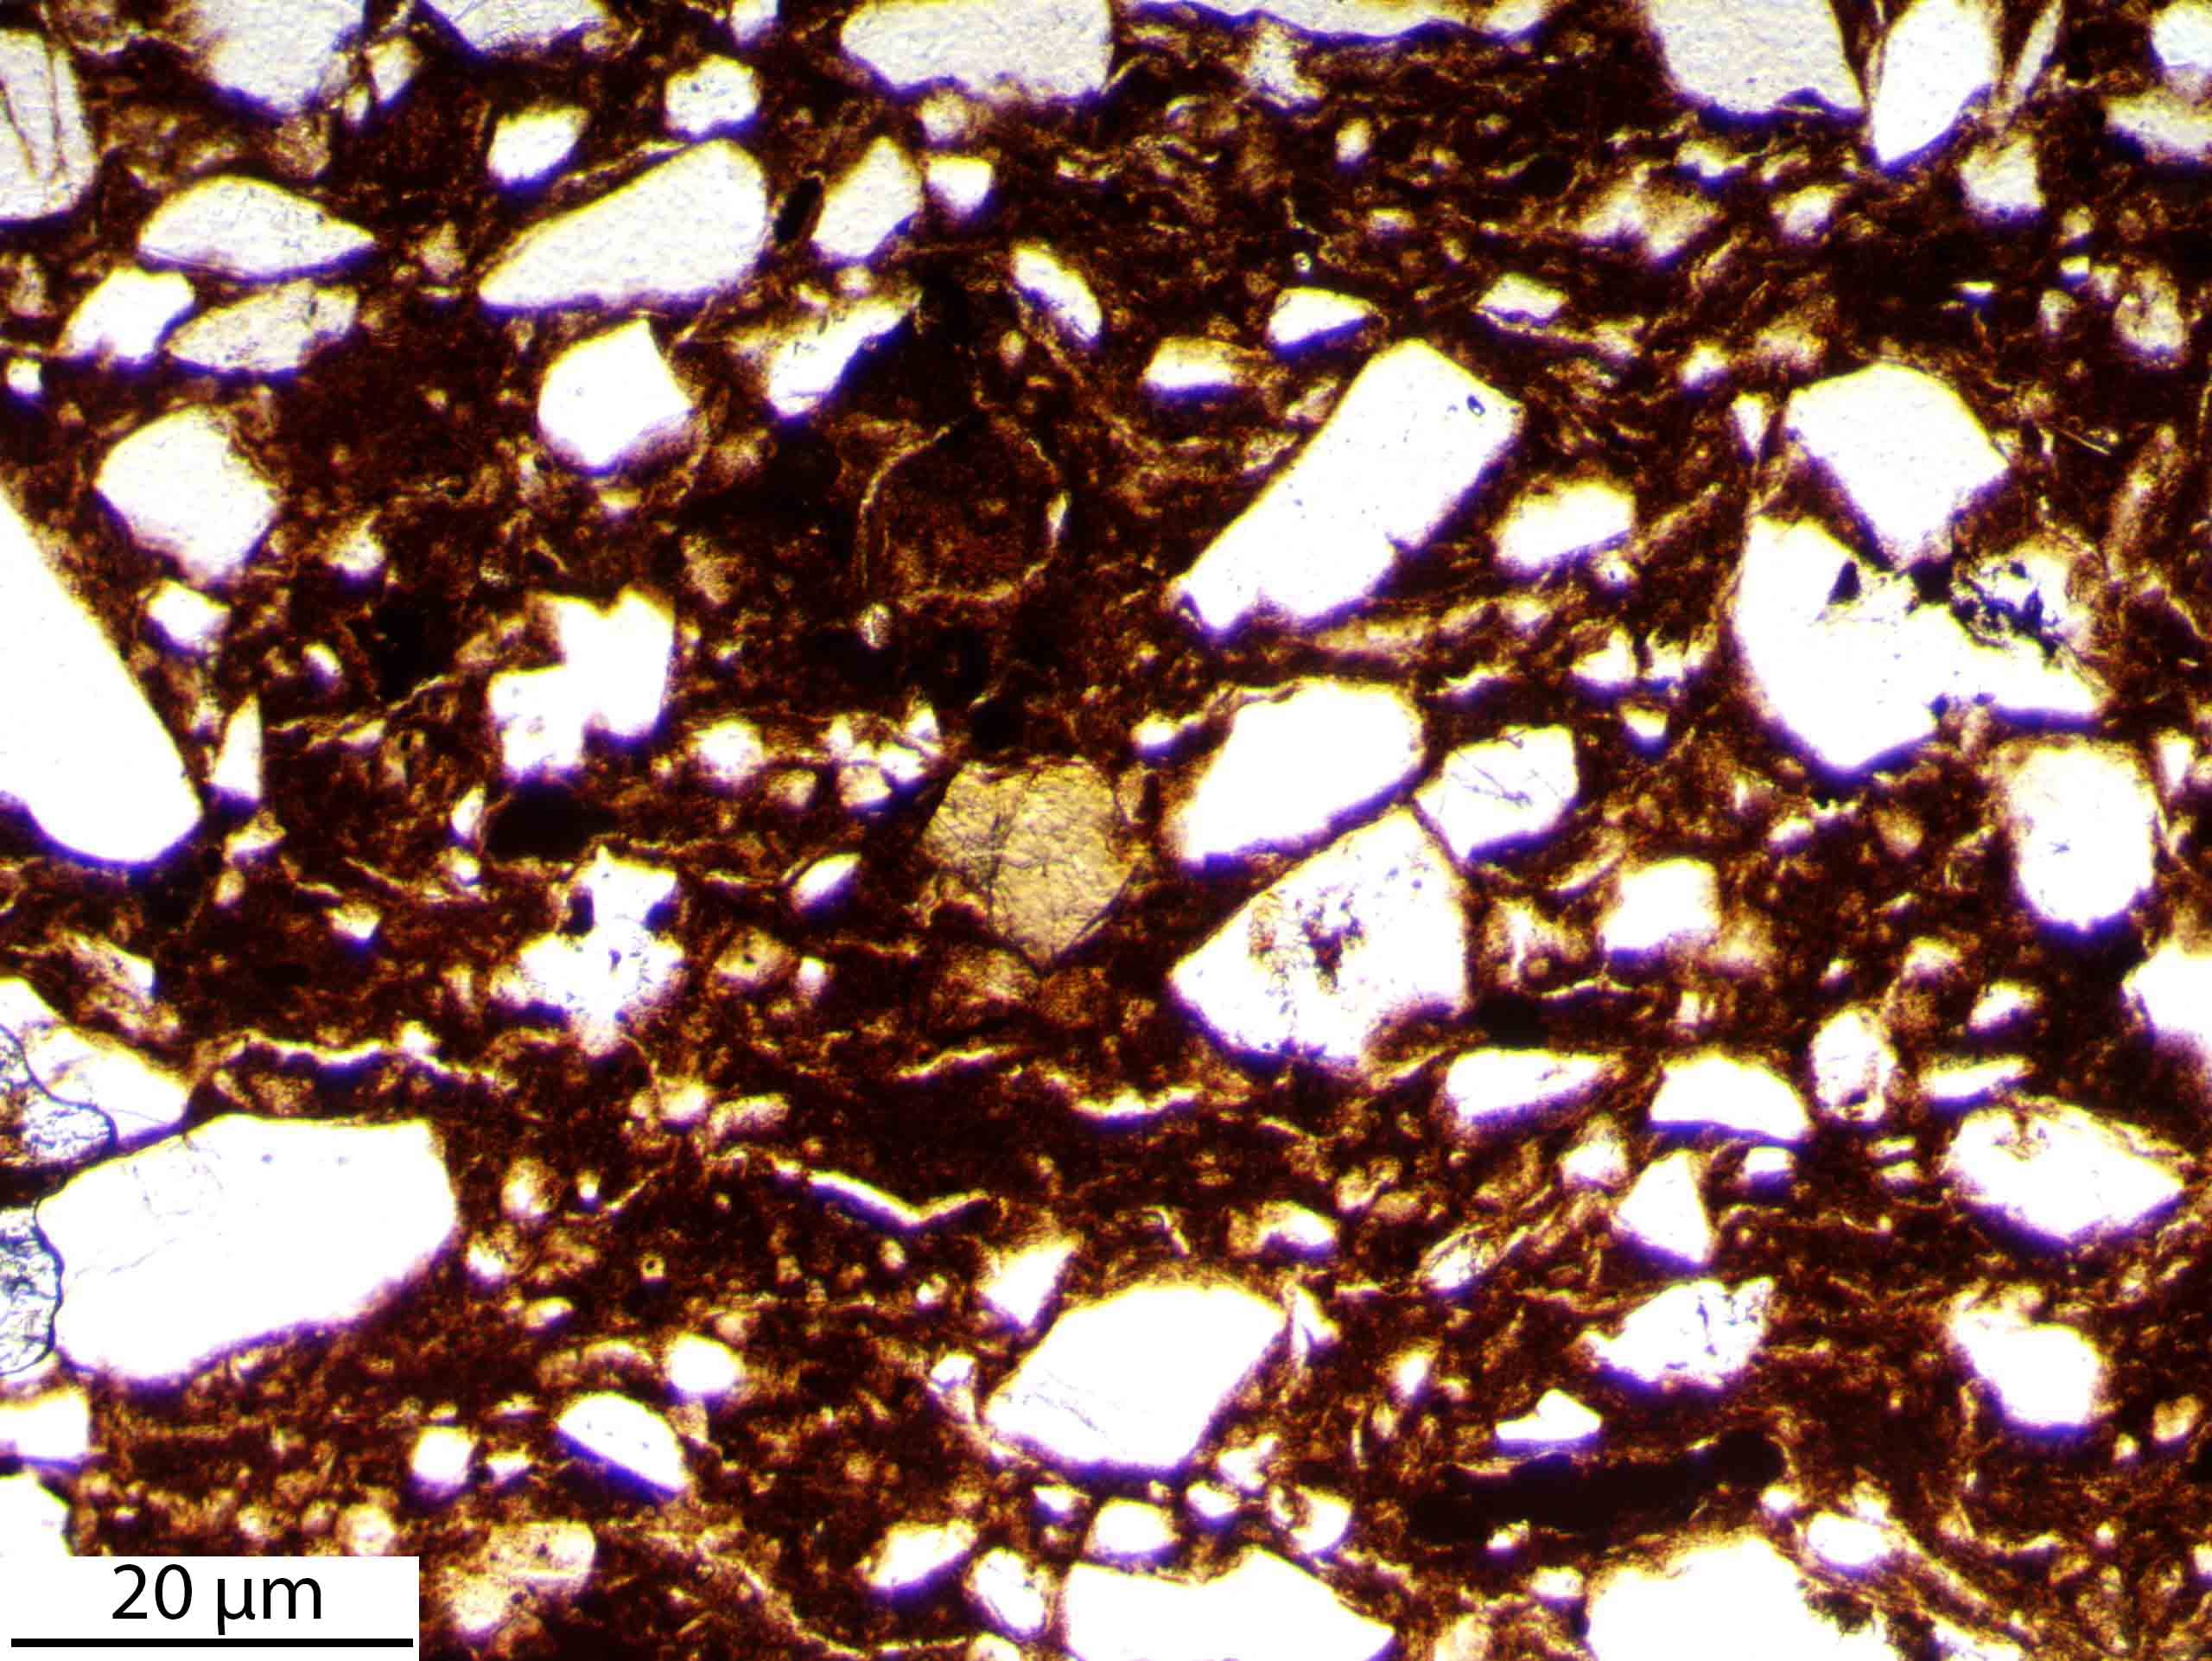
\includegraphics[width=\textwidth]{ThinSections/56-7_10x_PPL.jpg}
%		\caption{Staurolite [PPL]}
%	\end{subfigure}\hspace{.1em}\hfill
%	\begin{subfigure}[t]{.24\textwidth}
%		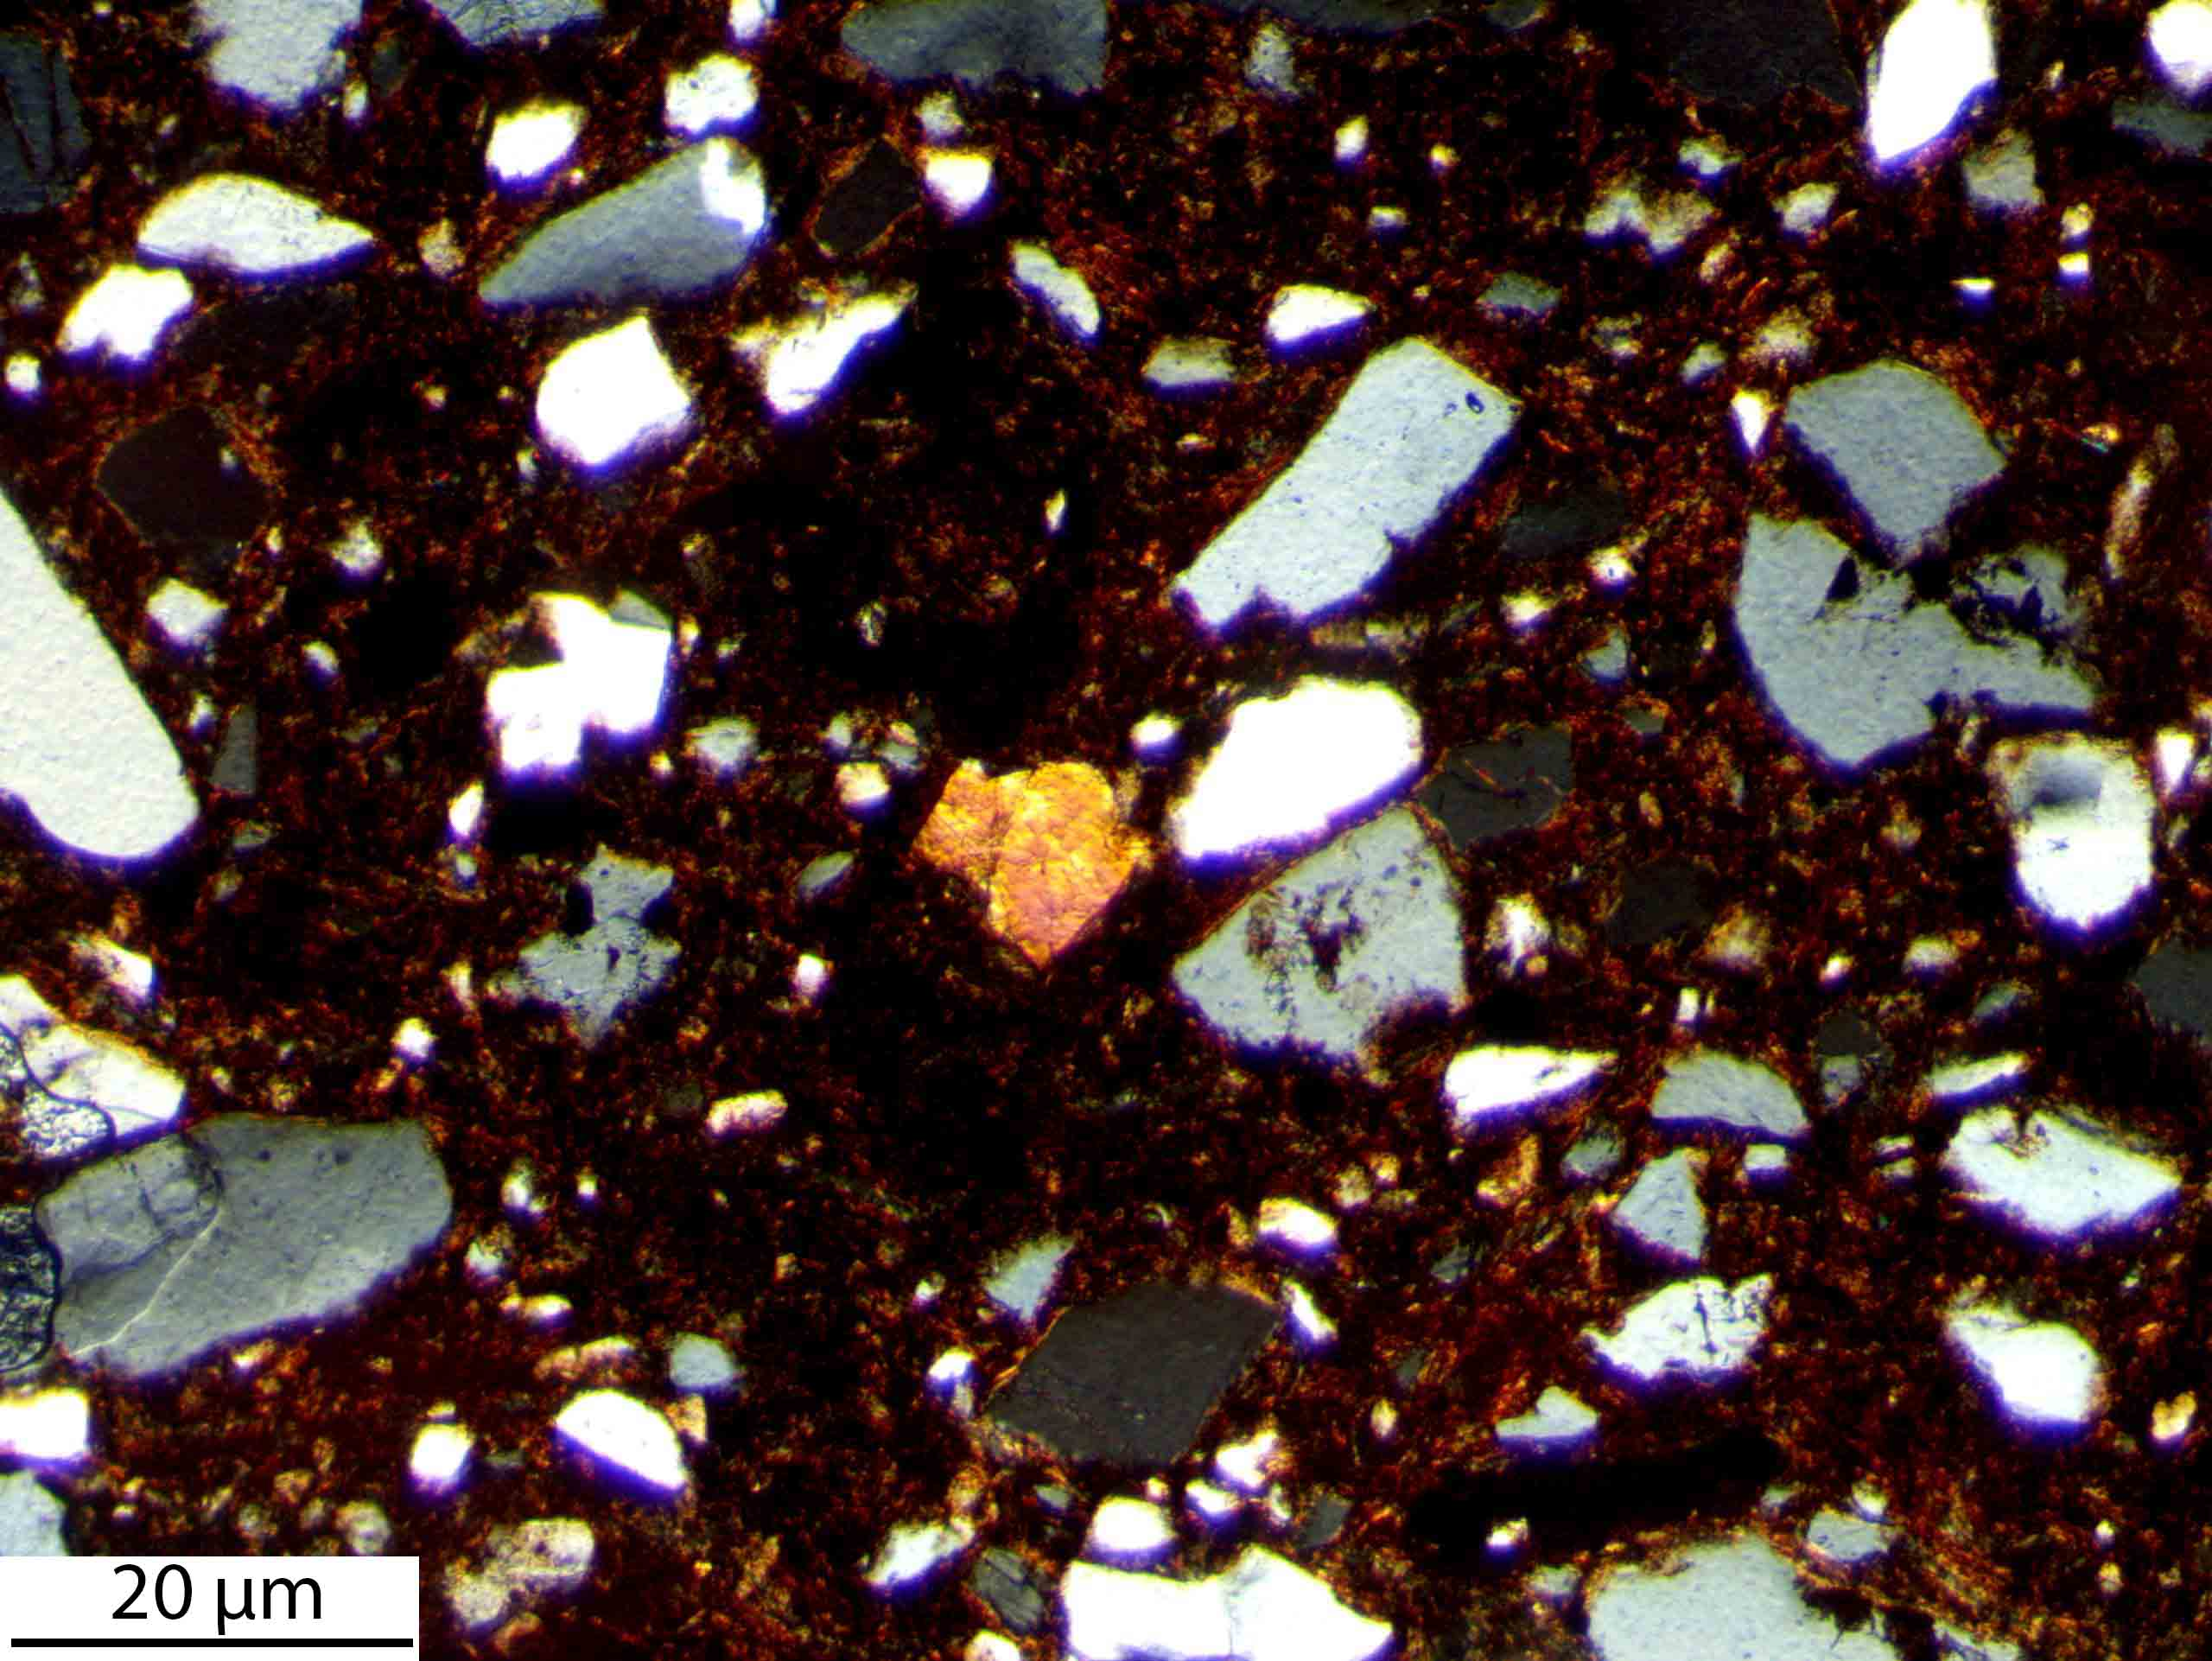
\includegraphics[width=\textwidth]{ThinSections/56-7_10x_XPL.jpg}
%		\caption{Staurolite [XPL]}
%	\end{subfigure}\hspace{.5em}\hfill
%	\begin{subfigure}[t]{.24\textwidth}
%		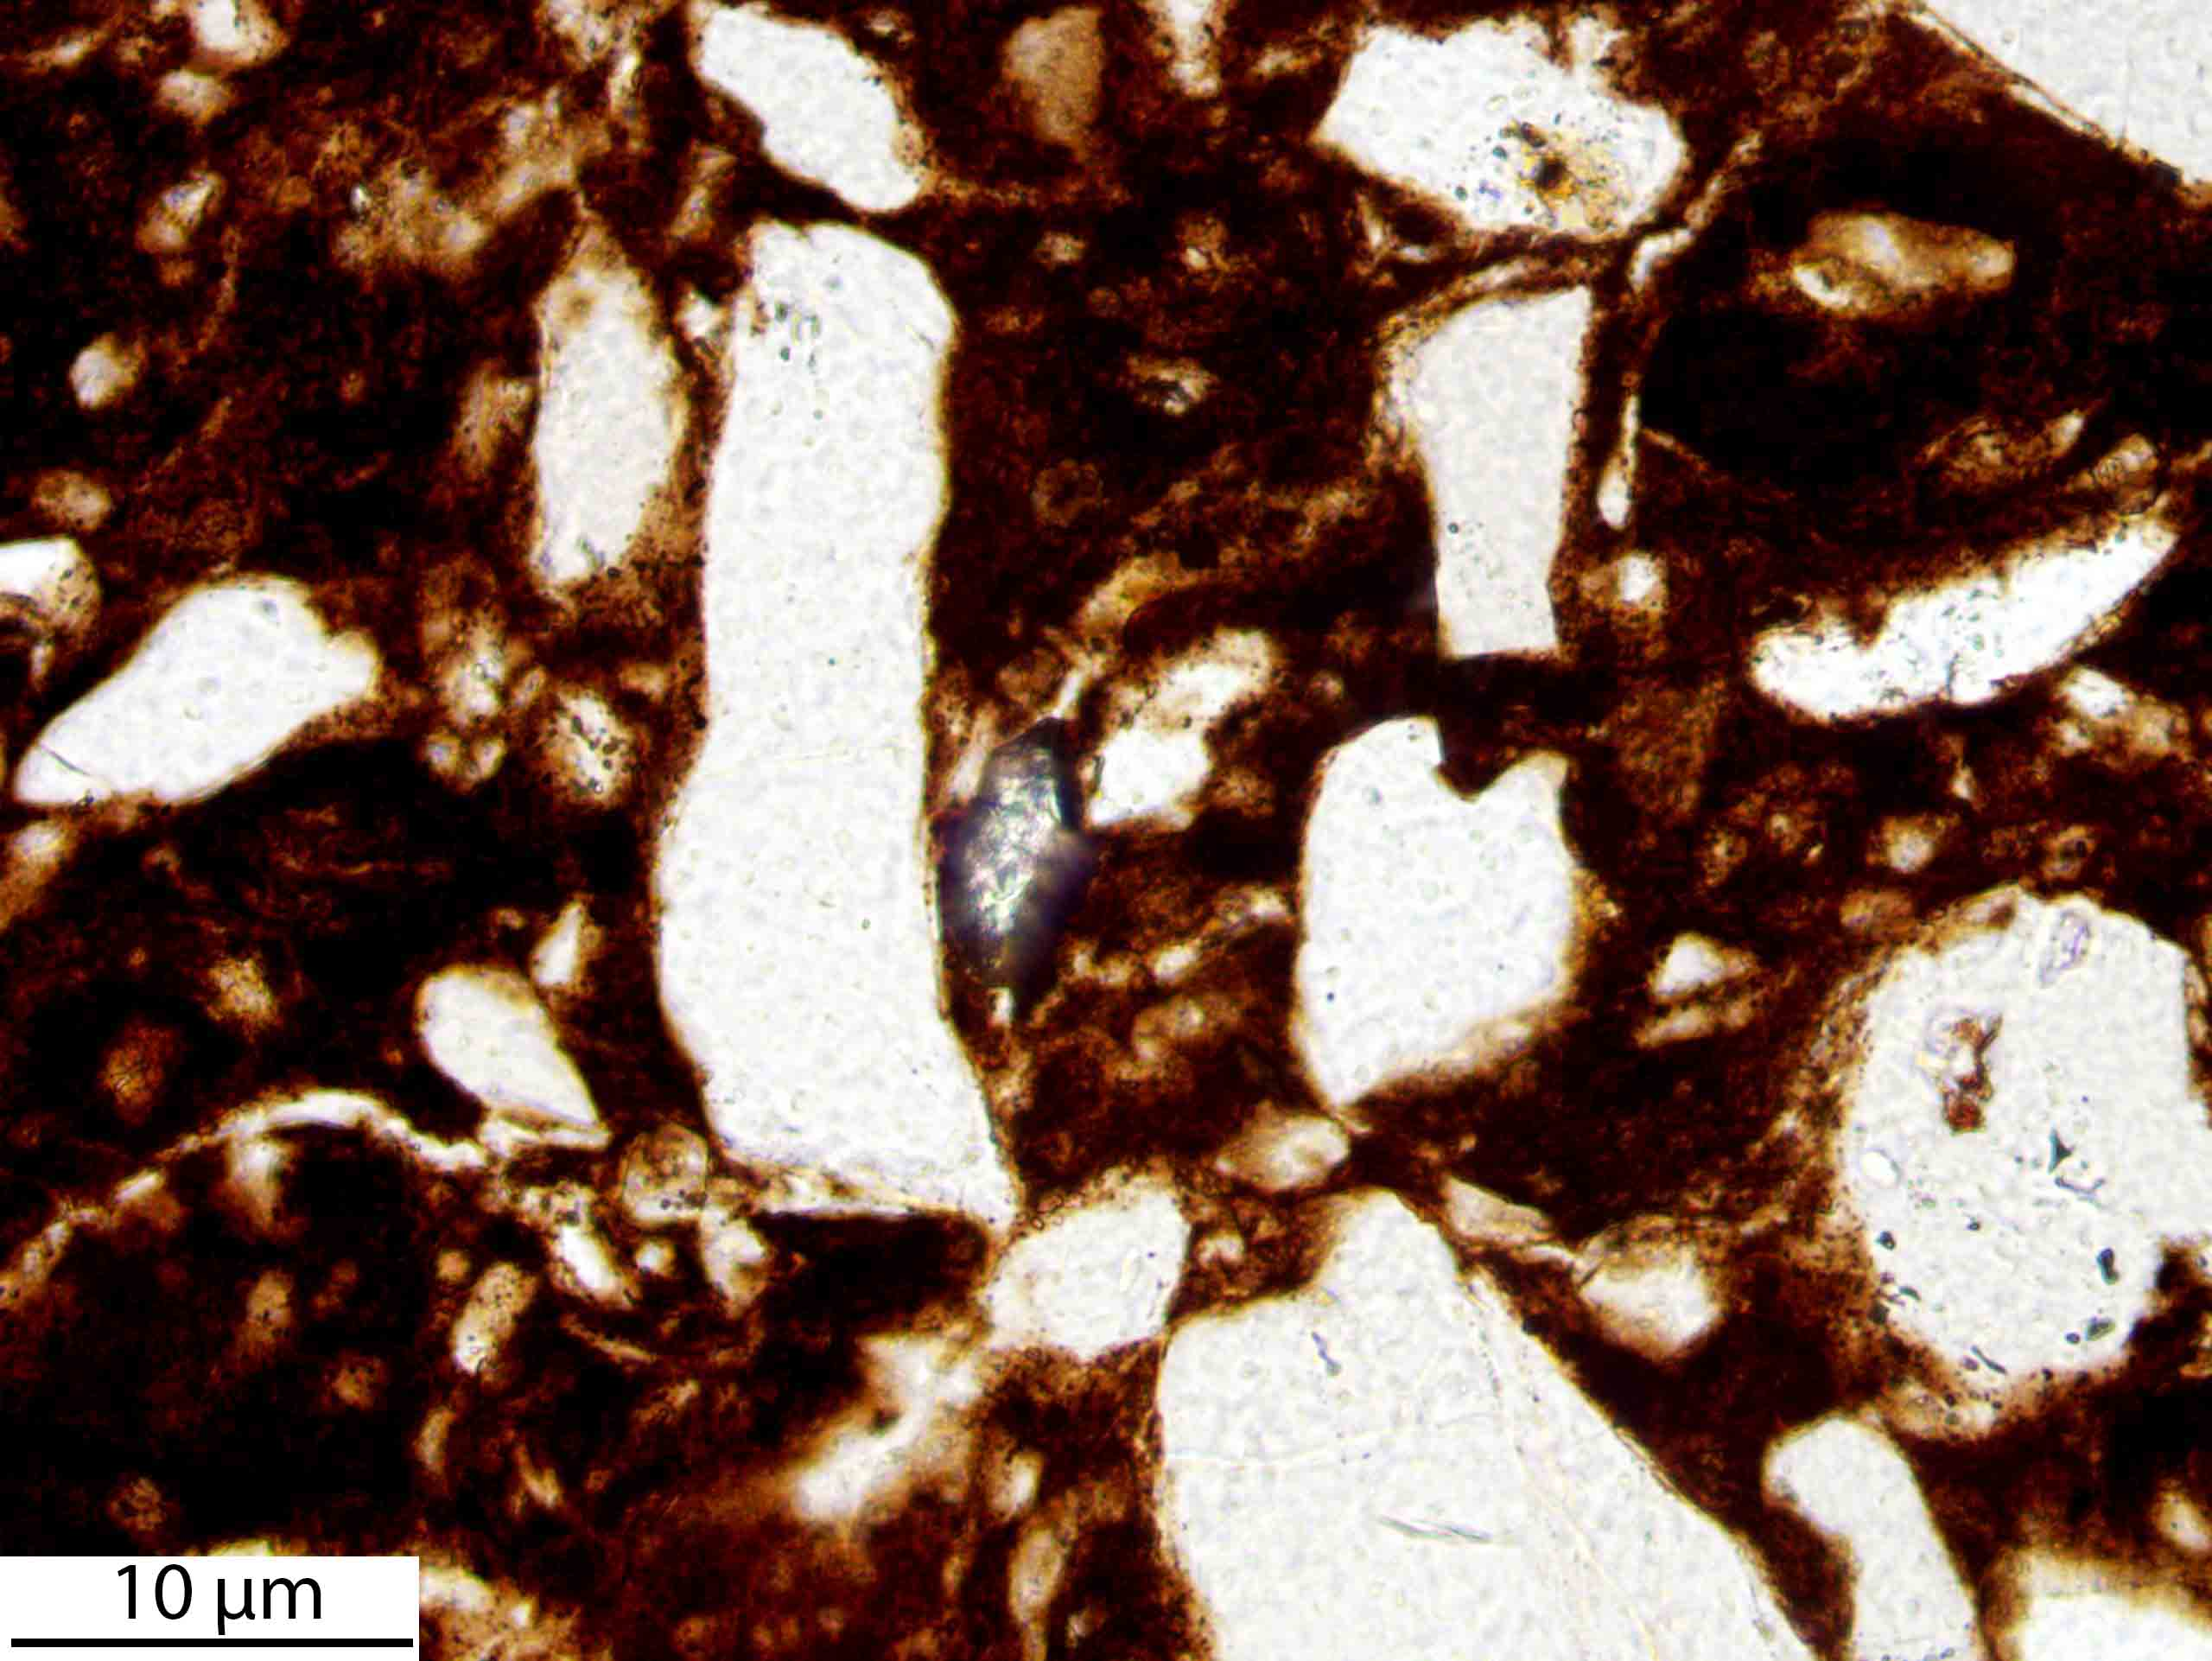
\includegraphics[width=\textwidth]{ThinSections/56-5_20x_PPL.jpg}
%		\caption{Zircon [PPL]}
%	\end{subfigure}\hspace{.1em}\hfill
%	\begin{subfigure}[t]{.24\textwidth}
%		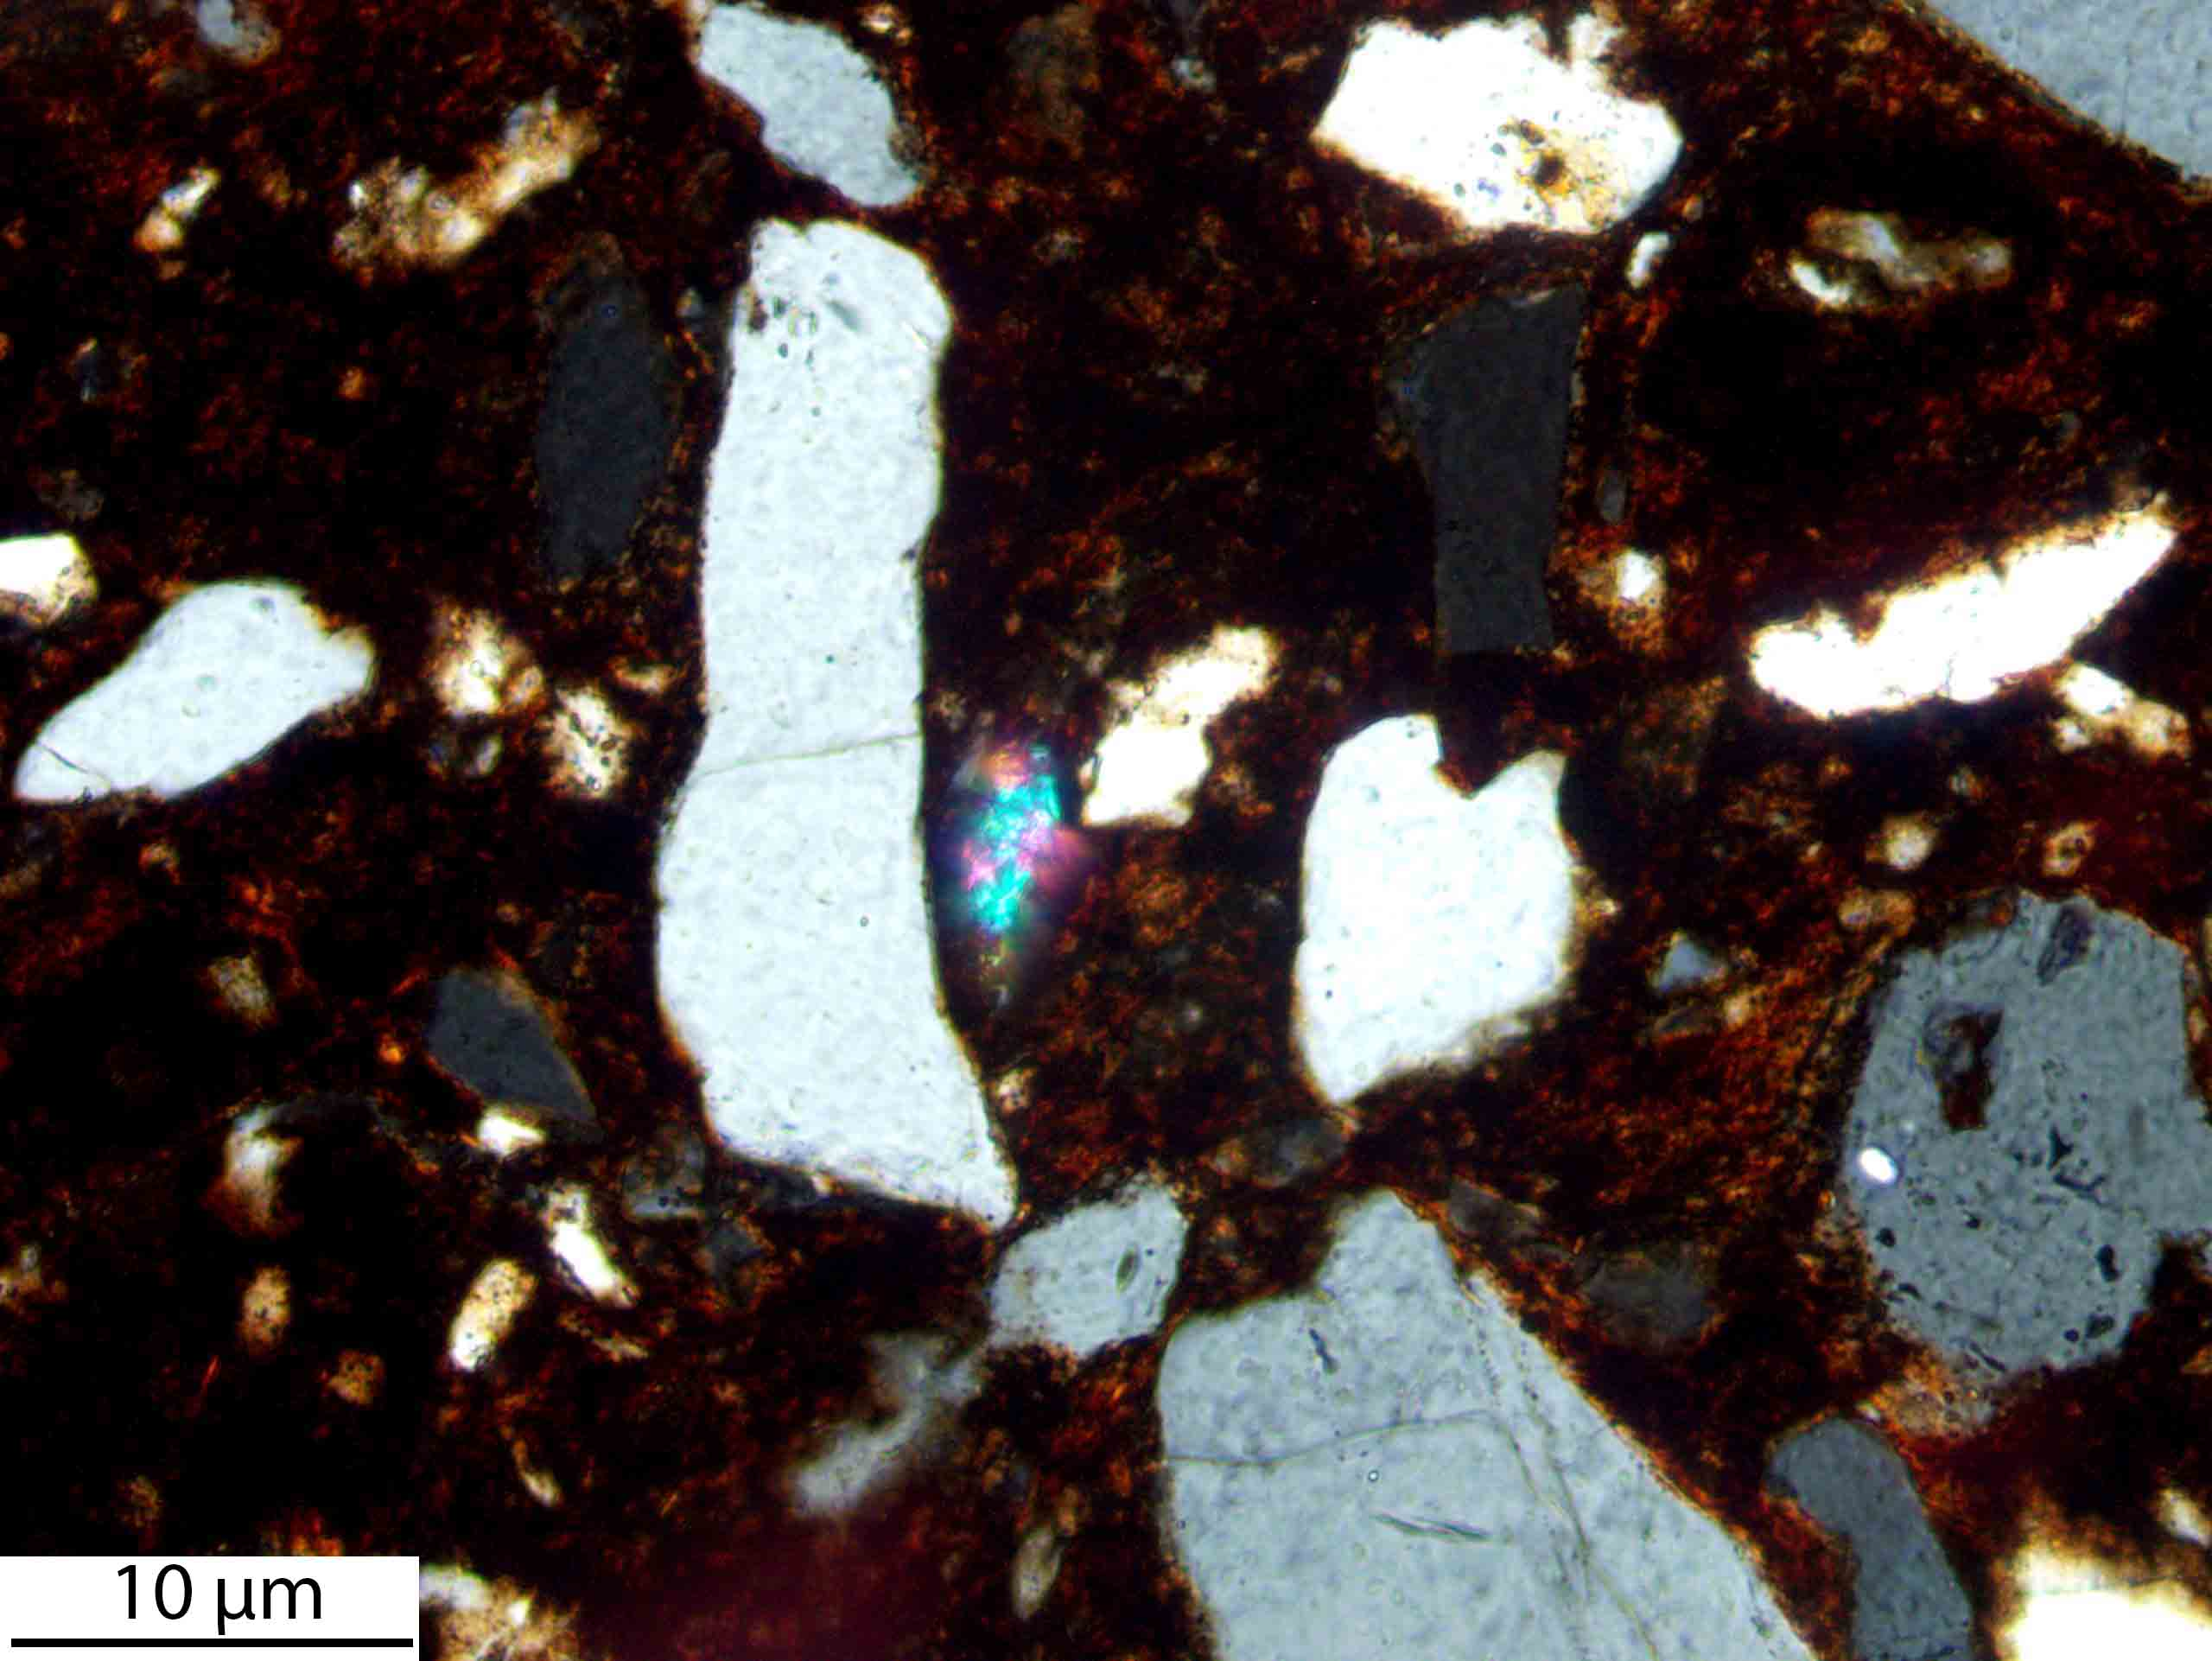
\includegraphics[width=\textwidth]{ThinSections/56-5_20x_XPL.jpg}
%		\caption{Zircon [XPL]}
%	\end{subfigure}
	\caption{}
	\label{fig:56_pik}
\end{figure}

\newpage\subsection{PIK~87/1-9:5 \citep[pik\#54; Fig.~\ref{fig:pik.pottery}.4; Pikunda-Munda style;][428 Pl.~47.7]{Seidensticker.2021e}}

\begin{multicols}{2}
\noindent The samples fine fraction (light yellow, reddish brown and dark brown [PPL]) is heterogeneous and non-calcareous with stipple-speckled b-fabric. Voids are more pronounced towards the inside of the sherd and generally wall-parallel in relation to the plane of the section. The coarse fraction is dominated by densely packed sponge spicules, mostly transversely cut, and fine sub-angular quartz appearing in a unimodal grain-size distribution. Muscovite and zircon are occasionally present. The c/f-related distribution pattern is single-spaced porphyric.
\end{multicols}

%\vfill
\begin{figure}[H]
	\centering
	\begin{subfigure}[t]{.49\textwidth}
		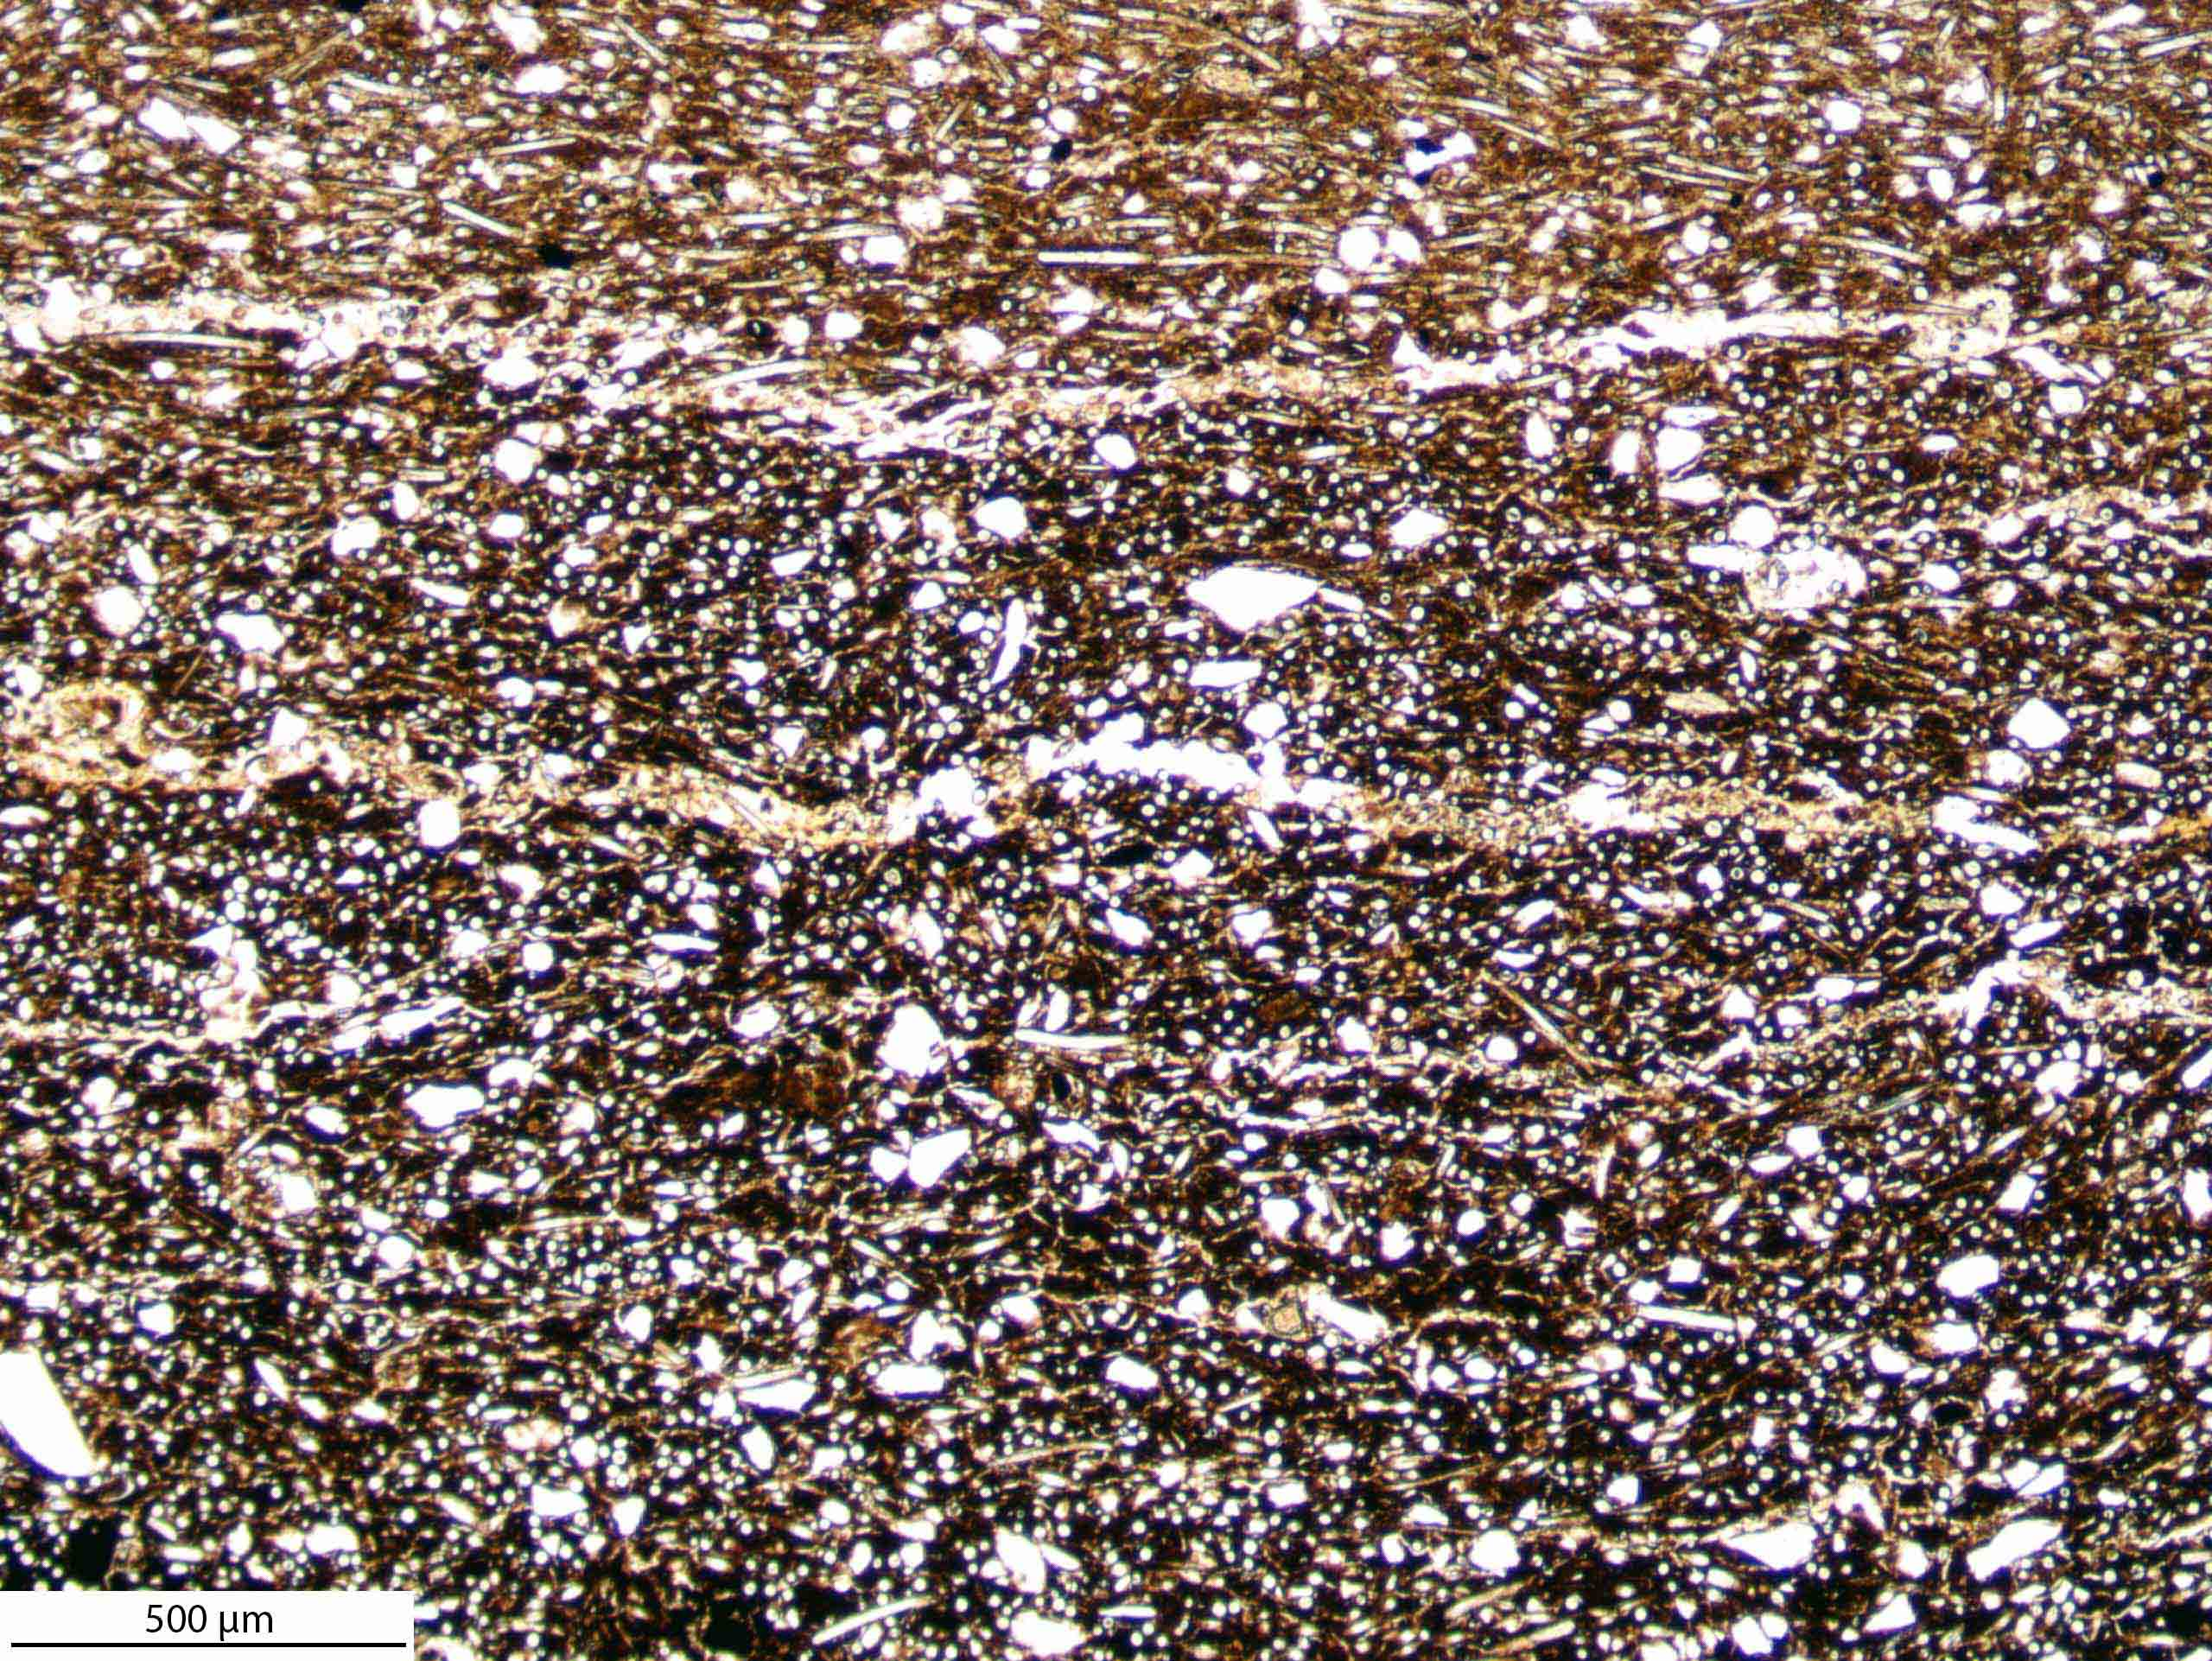
\includegraphics[width=\textwidth]{ThinSections/54-1_4x_PPL.jpg}
		\caption{[PPL]}
	\end{subfigure}\hspace{.5em}\hfill
	\begin{subfigure}[t]{.49\textwidth}
		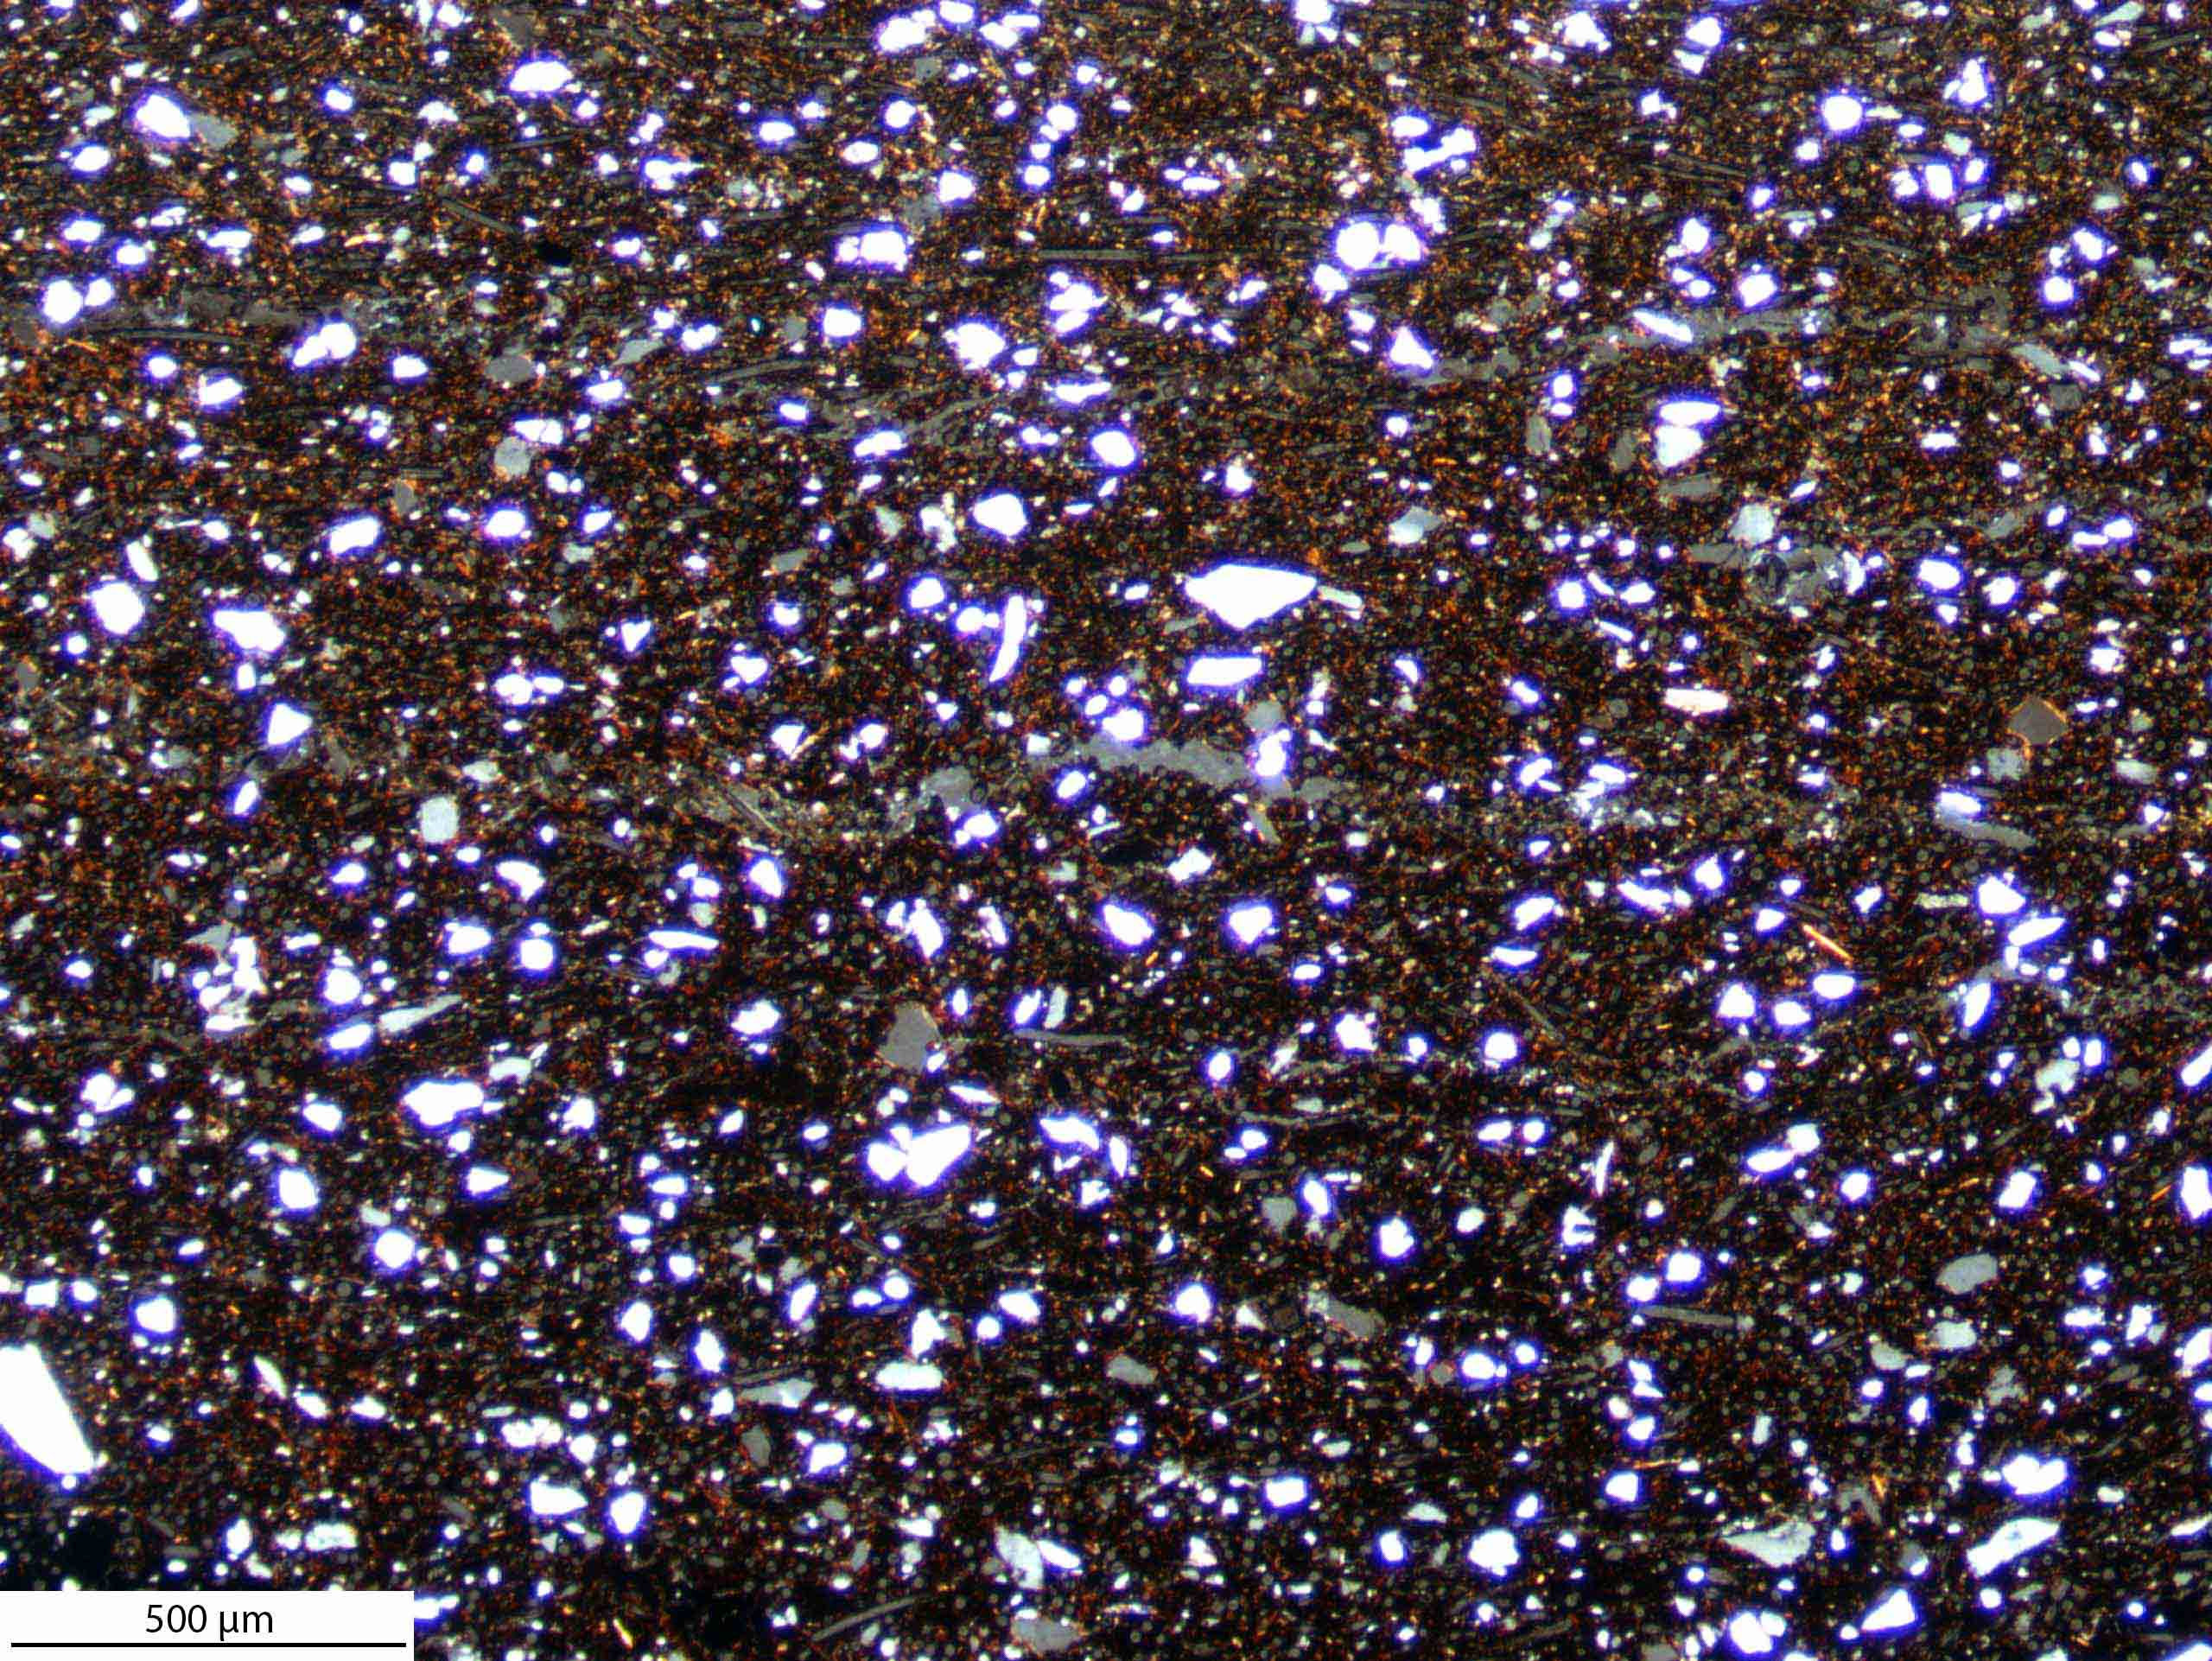
\includegraphics[width=\textwidth]{ThinSections/54-1_4x_XPL.jpg}
		\caption{[XPL]}
	\end{subfigure}
	\begin{subfigure}[t]{.32\textwidth}
		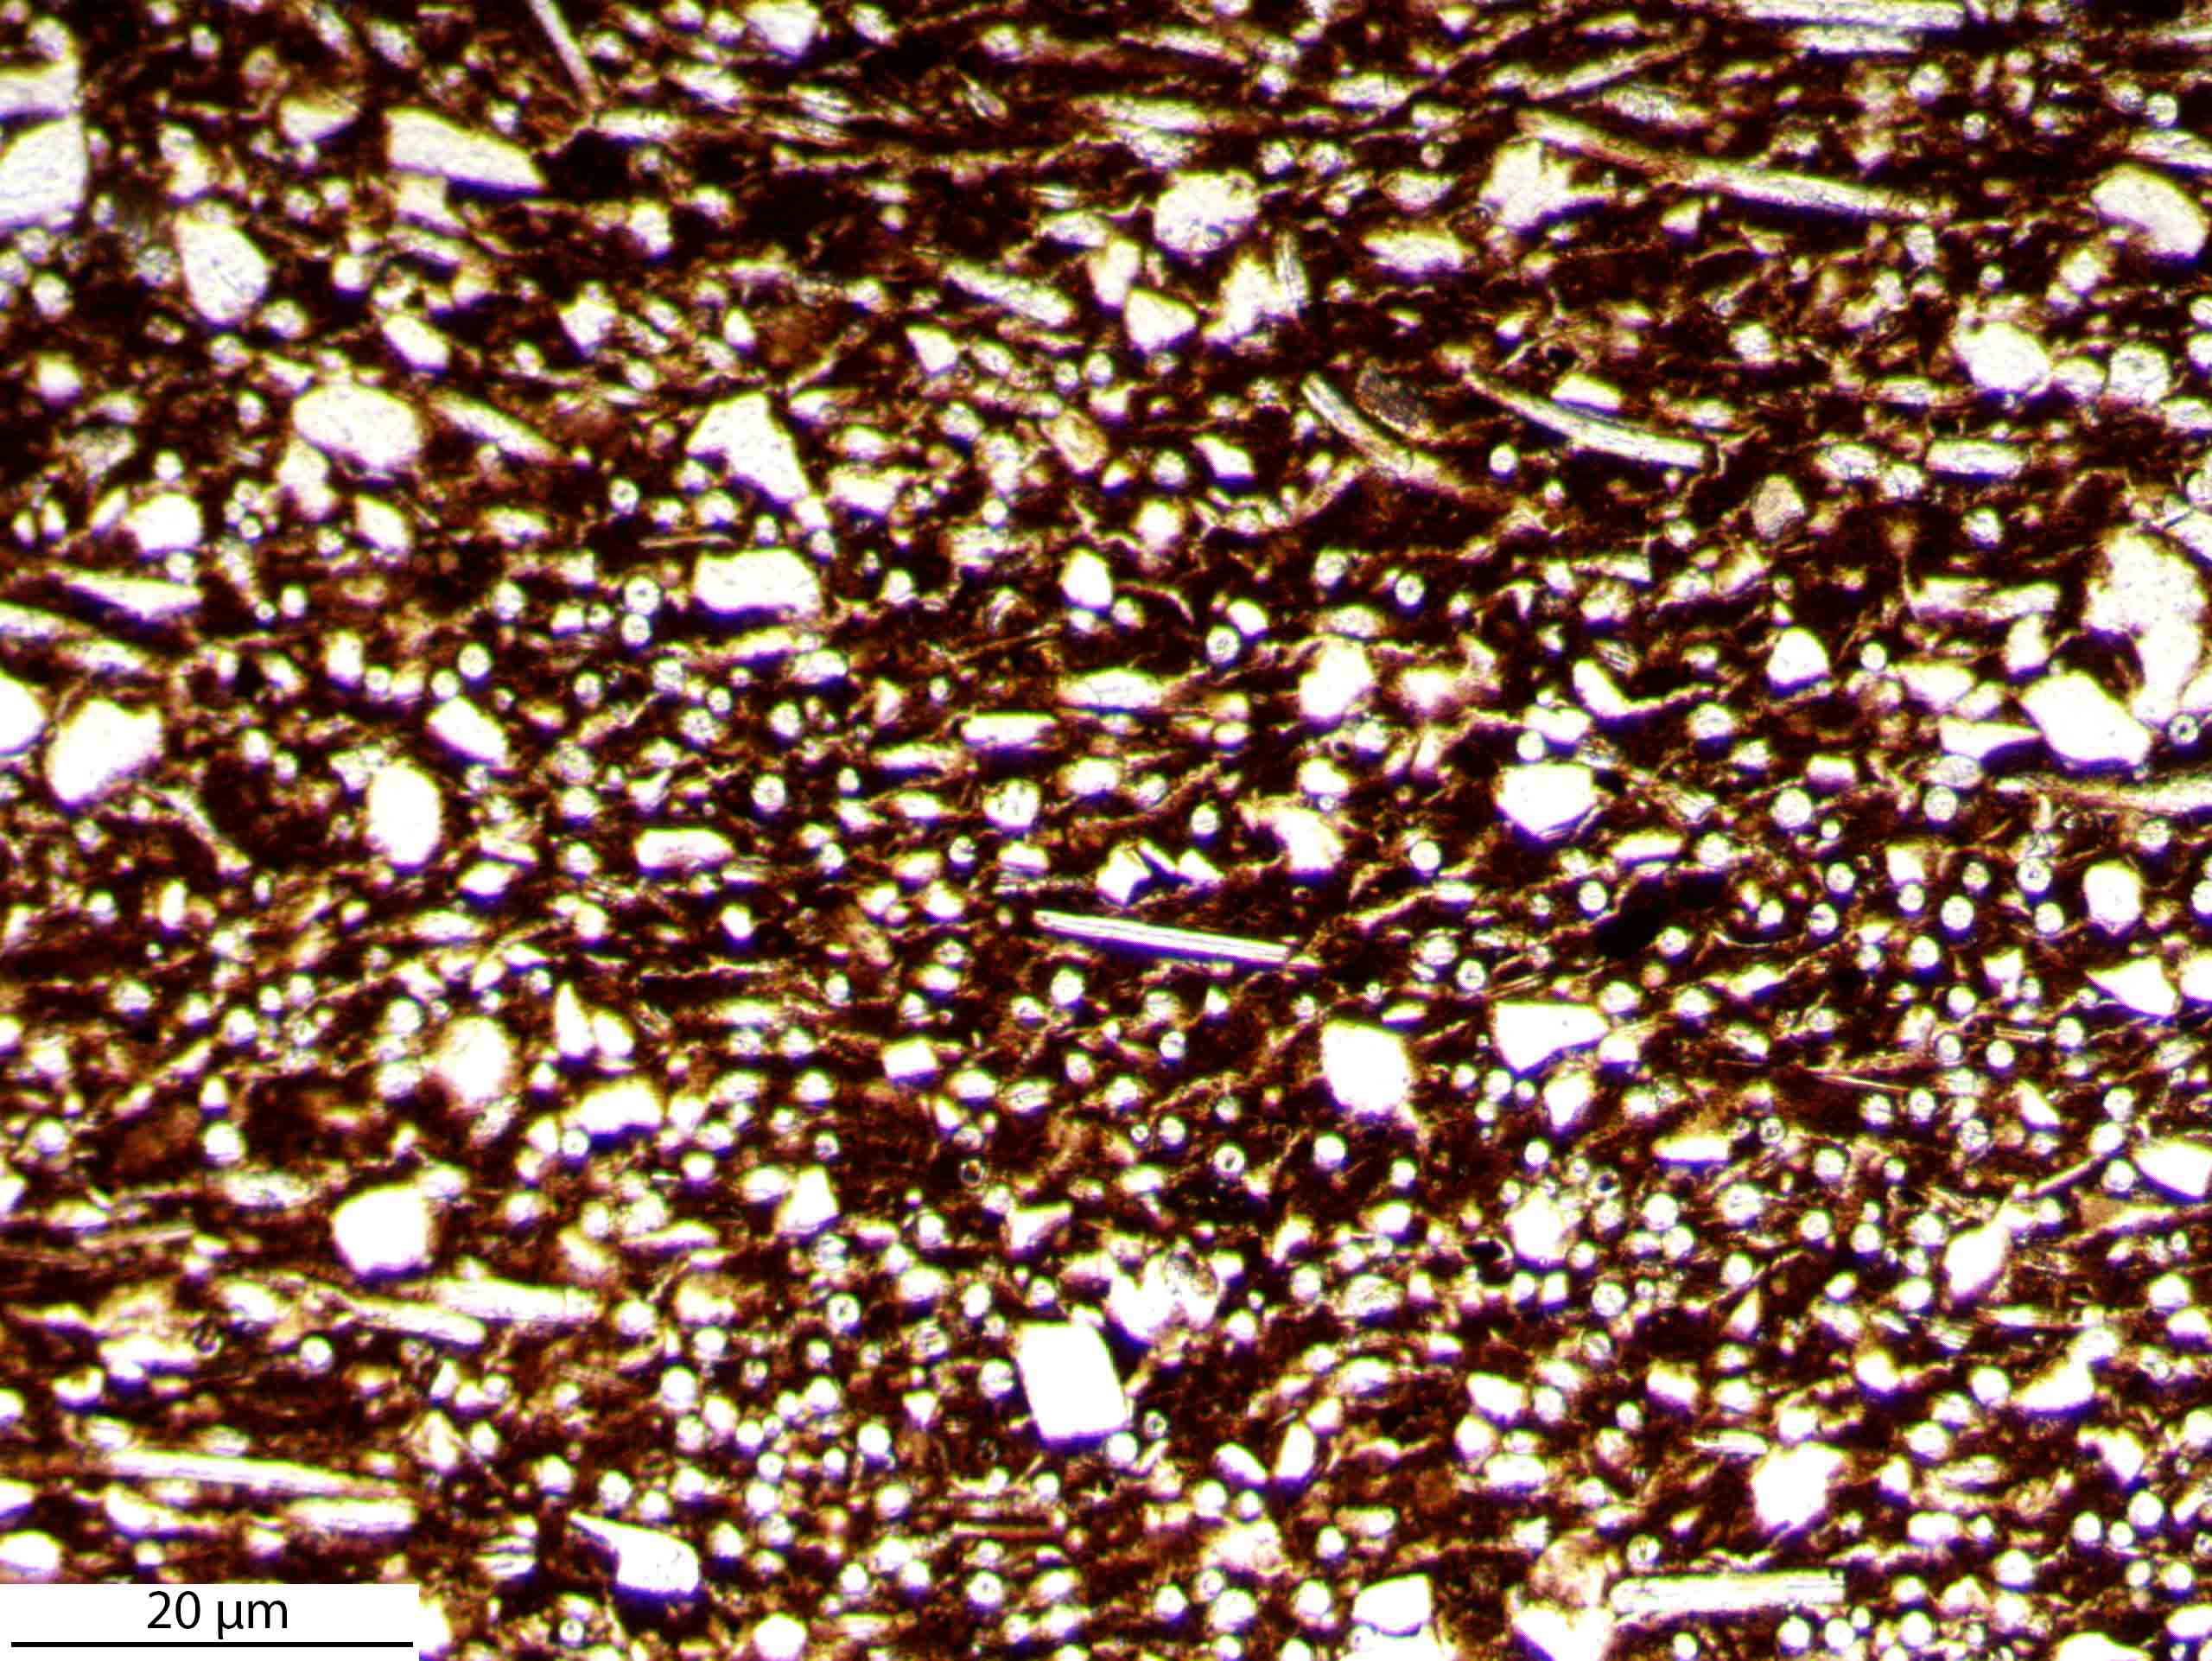
\includegraphics[width=\textwidth]{ThinSections/54-6_10x_PPL.jpg}
		\caption{Detail [PPL]}
	\end{subfigure}\hspace{.5em}\hfill
%	\begin{subfigure}[t]{.49\textwidth}
%		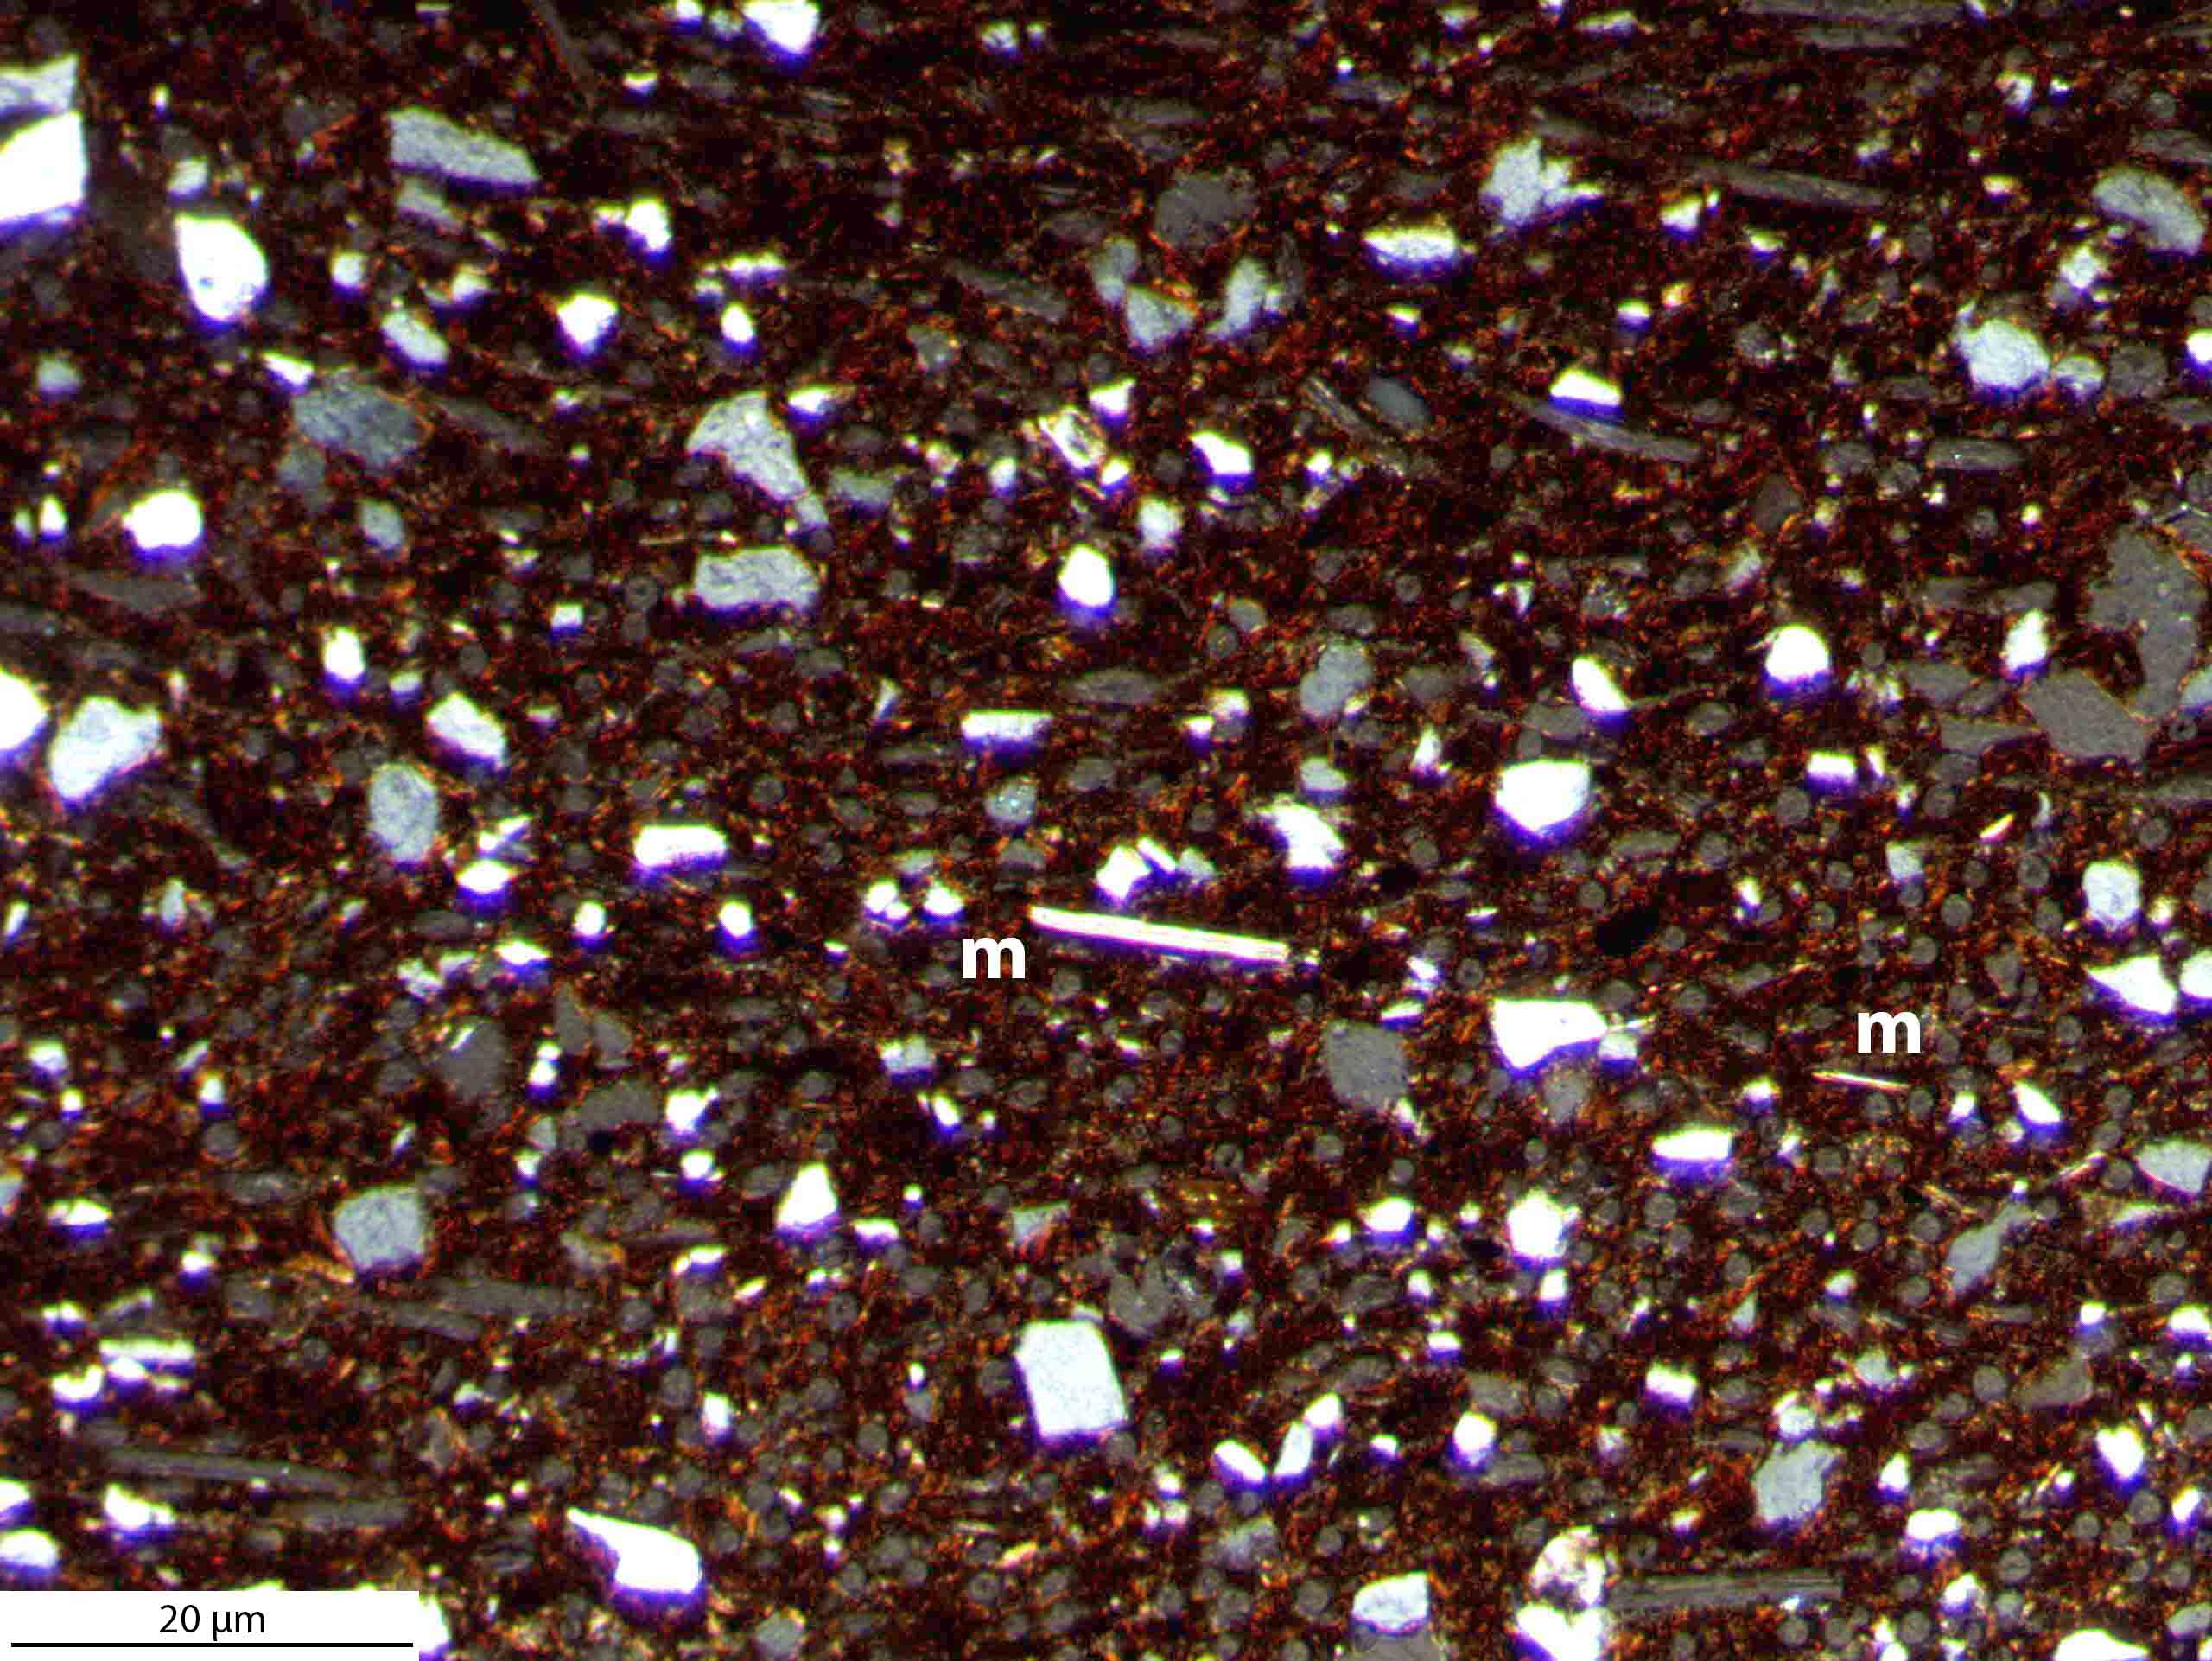
\includegraphics[width=\textwidth]{ThinSections/54-6_10x_XPL.jpg}
%		\caption{Muscovite [XPL]}
%	\end{subfigure}
	\begin{subfigure}[t]{.32\textwidth}
		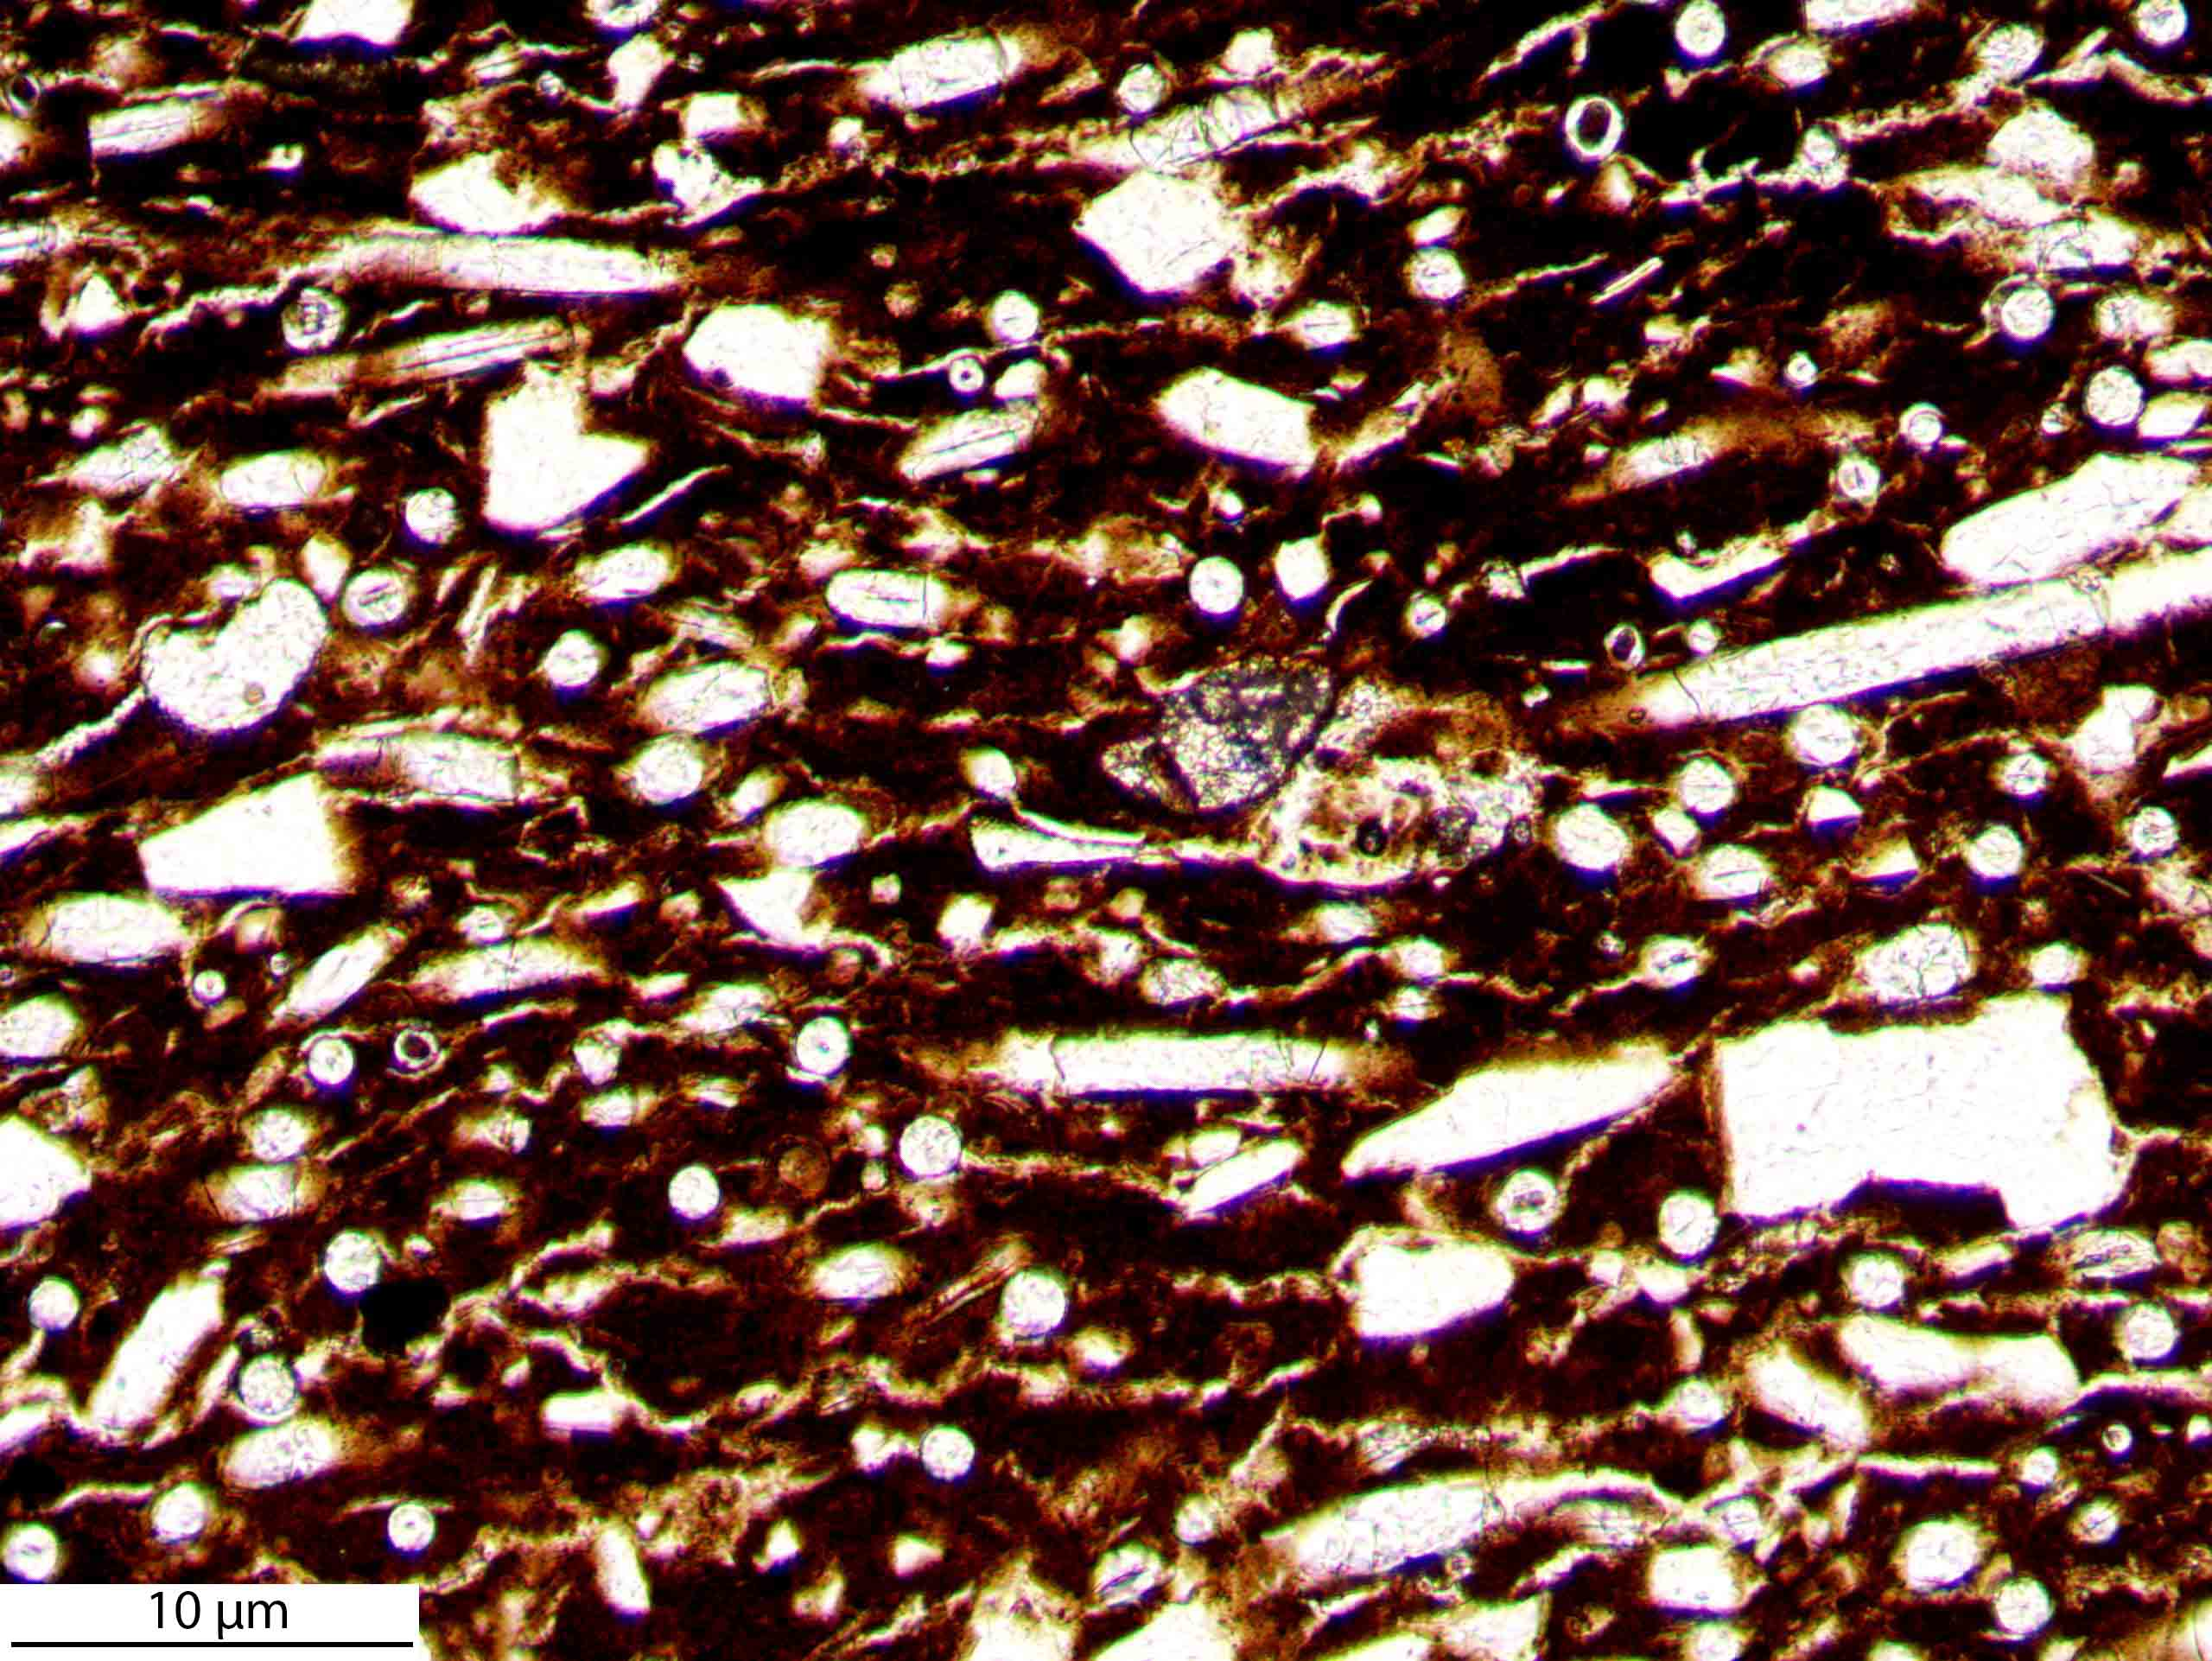
\includegraphics[width=\textwidth]{ThinSections/54-3_20x_PPL.jpg}
		\caption{Detail [PPL]}
	\end{subfigure}\hspace{.5em}\hfill
	\begin{subfigure}[t]{.32\textwidth}
		\includegraphics[width=\textwidth]{ThinSections/54-3_20x_XPL.jpg}
		\caption{Detail [XPL]}
	\end{subfigure}
	\caption{}
	\label{fig:54_pik}
\end{figure}

\newpage\subsection{PIK~87/1-9:7 \citep[pik\#6; Fig.~\ref{fig:pik.pottery}.8; cf. Ngbanja style;][428 Pl.~47.19]{Seidensticker.2021e}}

\begin{multicols}{2}
\noindent The fine fraction (yellowish to reddish-brown [PPL]) is homogeneous, non-calcareous with stipple-speckled b-fabric. Voids are numerous but narrow and organized in a diagonal (S) configuration in respect to the plane of the section. The coarse fraction is dominated by angular quartz and rock fragments (sandstone) in a bimodal grain-size distribution. The quartz fraction is partially comprised of runiquartz. Also common are dark-brown to opaque (PPL) iron-rich inclusions (soil deposits). Rarely present are muscovite and biotite. The c/f-related distribution pattern is single-spaced porphyric.
\end{multicols}

% very rarely present is muscovite, biotite and tourmaline.

%\vfill
\begin{figure}[H]
	\centering
	\begin{subfigure}[t]{.49\textwidth}
		\includegraphics[width=\textwidth]{ThinSections/6-1_4x_PPL.jpg}
		\caption{[PPL]}
	\end{subfigure}\hspace{.5em}\hfill
	\begin{subfigure}[t]{.49\textwidth}
		\includegraphics[width=\textwidth]{ThinSections/6-1_4x_XPL.jpg}
		\caption{[XPL]}
	\end{subfigure}
	\begin{subfigure}[t]{.24\textwidth}
		\includegraphics[width=\textwidth]{ThinSections/6-3_4x_PPL.jpg}
		\caption{Rock fragment [PPL]}
	\end{subfigure}\hspace{.1em}\hfill
	\begin{subfigure}[t]{.24\textwidth}
		\includegraphics[width=\textwidth]{ThinSections/6-3_4x_XPL.jpg}
		\caption{Rock fragment [XPL]}
	\end{subfigure}\hspace{.5em}\hfill
	\begin{subfigure}[t]{.24\textwidth}
		\includegraphics[width=\textwidth]{ThinSections/6-5_4x_PPL.jpg}
		\caption{Rock fragment [PPL]}
	\end{subfigure}\hspace{.1em}\hfill
	\begin{subfigure}[t]{.24\textwidth}
		\includegraphics[width=\textwidth]{ThinSections/6-5_4x_XPL.jpg}
		\caption{Rock fragment [XPL]}
	\end{subfigure}
%	\begin{subfigure}[t]{.24\textwidth}
%		\includegraphics[width=\textwidth]{ThinSections/6-2_20x_PPL.jpg}
%		\caption{[PPL]}
%	\end{subfigure}\hspace{.1em}\hfill
%	\begin{subfigure}[t]{.24\textwidth}
%		\includegraphics[width=\textwidth]{ThinSections/6-2_20x_XPL.jpg}
%		\caption{[XPL]}
%	\end{subfigure}\hspace{.5em}\hfill
%	\begin{subfigure}[t]{.24\textwidth}
%		\includegraphics[width=\textwidth]{ThinSections/6-4_20x_PPL.jpg}
%		\caption{Tourmaline [PPL]}
%	\end{subfigure}\hspace{.1em}\hfill
%	\begin{subfigure}[t]{.24\textwidth}
%		\includegraphics[width=\textwidth]{ThinSections/6-4_20x_XPL.jpg}
%		\caption{Tourmaline [XPL]}
%	\end{subfigure}
	\caption{}
	\label{fig:6_pik}
\end{figure}

\newpage\subsection{PIK~87/1-12:1 \citep[pik\#53; Fig.~\ref{fig:pik.pottery}.2; Lusako style;][426 Pl.~45.16]{Seidensticker.2021e}}

\begin{multicols}{2}
\noindent The fine fraction is homogeneous and non-calcareous (reddish brown [PPL]) with undifferentiated b-fabric. Voids are rare, rounded, and in a diagonal (Z) configuration. The coarse fraction is dominated by densely packed sponge spicules (single spaced porphyric), mostly transversely cut in respect to the plane of the section, and sub-angular quartz. The quartz fraction is also shows diagonal orientations. Muscovite, biotite and tourmaline is very rarely present. The c/f-related distribution pattern is single- to double-spaced porphyric.
\end{multicols}

%\vfill
\begin{figure}[H]
	\centering
	\begin{subfigure}[t]{.49\textwidth}
		\includegraphics[width=\textwidth]{ThinSections/53-1_4x_PPL.jpg}
		\caption{[PPL]}
	\end{subfigure}\hspace{.5em}\hfill
	\begin{subfigure}[t]{.49\textwidth}
		\includegraphics[width=\textwidth]{ThinSections/53-1_4x_XPL.jpg}
		\caption{[XPL]}
	\end{subfigure}
	\begin{subfigure}[t]{.32\textwidth}
		\includegraphics[width=\textwidth]{ThinSections/53-2_20x_PPL.jpg}
		\caption{Detail [PPL]}
	\end{subfigure}\hspace{.1em}\hfill
%	\begin{subfigure}[t]{.49\textwidth}
%		\includegraphics[width=\textwidth]{ThinSections/53-2_20x_XPL.jpg}
%		\caption{Muscovite [XPL]}
%	\end{subfigure}
	\begin{subfigure}[t]{.32\textwidth}
		\includegraphics[width=\textwidth]{ThinSections/53-3_20x_PPL.jpg}
		\caption{Detail [PPL]}
	\end{subfigure}\hspace{.1em}\hfill
	\begin{subfigure}[t]{.32\textwidth}
		\includegraphics[width=\textwidth]{ThinSections/53-3_20x_XPL.jpg}
		\caption{Detail [XPL]}
	\end{subfigure}
%	\begin{subfigure}[t]{.24\textwidth}
%		\includegraphics[width=\textwidth]{ThinSections/53-4_20x_PPL.jpg}
%		\caption{Staurolite [PPL]}
%	\end{subfigure}\hspace{.1em}\hfill
%	\begin{subfigure}[t]{.24\textwidth}
%		\includegraphics[width=\textwidth]{ThinSections/53-4_20x_XPL.jpg}
%		\caption{Staurolite [XPL]}
%	\end{subfigure}
	\caption{}
	\label{fig:53_pik}
\end{figure}

\newpage\subsection{PIK~87/2-1:40 \citep[pik\#99; Fig.~\ref{fig:pik.pottery}.12; Ebambe style;][430 Pl.~49.10]{Seidensticker.2021e}}

\begin{multicols}{2}
\noindent The sample shows a homogeneous, non-calcareous fine fraction (reddish brown [PPL]) with undifferentiated b-fabric. Voids are predominantly oriented wall-parallel with respect to the plane of the section. The main constituent of the coarse fraction are densely packed sponge spicules that are mostly cut transversely. Also very common is sub-angular quartz. Also present is charred organic matter (c--e). Rarely present is muscovite. The c/f-related distribution pattern is single-spaced porphyric (double-spaced to open porphyric if only quartz grains are regarded as coarse material).
\end{multicols}

%\vfill
\begin{figure}[H]
	\centering
	\begin{subfigure}[t]{.49\textwidth}
		\includegraphics[width=\textwidth]{ThinSections/99-1_4x_PPL.jpg}
		\caption{[PPL]}
	\end{subfigure}\hspace{.5em}\hfill
	\begin{subfigure}[t]{.49\textwidth}
		\includegraphics[width=\textwidth]{ThinSections/99-1_4x_XPL.jpg}
		\caption{[XPL]}
	\end{subfigure}
	\begin{subfigure}[t]{.32\textwidth}
		\includegraphics[width=\textwidth]{ThinSections/99-1_20x_PPL.jpg}
		\caption{Charred plant matter [PPL]}
	\end{subfigure}\hspace{.1em}\hfill
	\begin{subfigure}[t]{.32\textwidth}
		\includegraphics[width=\textwidth]{ThinSections/99-2_20x_PPL.jpg}
		\caption{Charred plant matter [PPL]}
	\end{subfigure}\hspace{.1em}\hfill
	\begin{subfigure}[t]{.32\textwidth}
		\includegraphics[width=\textwidth]{ThinSections/99-4_10x_PPL.jpg}
		\caption{Charred plant matter [PPL]}
	\end{subfigure}
	\caption{}
	\label{fig:99_pik}
\end{figure}

\newpage\subsection{PIK~87/2-4:73 \citep[pik\#98; Fig.~\ref{fig:pik.pottery}.5; Pikunda-Munda style;][429 Pl.~48.25]{Seidensticker.2021e}}

\begin{multicols}{2}
\noindent The samples fine fraction is homogeneous and non-calcareous (yellowish-orange brown [PPL]) with undifferentiated b-fabric. Voids are very rare. The coarse fraction is defined by sponge spicules, often cut transversely in respect to the plane of the section. Also a common part of the coarse fraction is sub-angular quartz. The quartz fraction shows a bimodal grain-size distribution. Some of the larger quartz grains shows rolling extinction (e). Occasionally present are charred plant matter (c), muscovite and tourmaline. The c/f-related distribution pattern is single-spaced porphyric (single- to double-spaced porphyric if only quartz grains are regarded as coarse material).
\end{multicols}

%\vfill
\begin{figure}[H]
	\centering
	\begin{subfigure}[t]{.49\textwidth}
		\includegraphics[width=\textwidth]{ThinSections/98-1_4x_PPL.jpg}
		\caption{[PPL]}
	\end{subfigure}\hspace{.5em}\hfill
	\begin{subfigure}[t]{.49\textwidth}
		\includegraphics[width=\textwidth]{ThinSections/98-1_4x_XPL.jpg}
		\caption{[XPL]}
	\end{subfigure}
	\begin{subfigure}[t]{.32\textwidth}
		\includegraphics[width=\textwidth]{ThinSections/98-3_40x_PPL.jpg}
		\caption{Charred plant matter [PPL]}
	\end{subfigure}\hspace{.1em}\hfill
	\begin{subfigure}[t]{.32\textwidth}
		\includegraphics[width=\textwidth]{ThinSections/98-5_20x_PPL.jpg}
		\caption{Quartz with rolling extinction [PPL]}
	\end{subfigure}\hspace{.1em}\hfill
	\begin{subfigure}[t]{.32\textwidth}
		\includegraphics[width=\textwidth]{ThinSections/98-5_20x_XPL.jpg}
		\caption{Quartz with rolling extinction [XPL]}
	\end{subfigure}
%	\begin{subfigure}[t]{.24\textwidth}
%		\includegraphics[width=\textwidth]{ThinSections/98-2_40x_PPL.jpg}
%		\caption{Muscovite [PPL]}
%	\end{subfigure}\hspace{.1em}\hfill
%	\begin{subfigure}[t]{.24\textwidth}
%		\includegraphics[width=\textwidth]{ThinSections/98-2_40x_XPL.jpg}
%		\caption{Muscovite [XPL]}
%	\end{subfigure}\hspace{.5em}\hfill
%	\begin{subfigure}[t]{.24\textwidth}
%		\includegraphics[width=\textwidth]{ThinSections/98-4_40x_PPL.jpg}
%		\caption{Zircon [PPL]}
%	\end{subfigure}\hspace{.5em}\hfill
%	\begin{subfigure}[t]{.24\textwidth}
%		\includegraphics[width=\textwidth]{ThinSections/98-4_40x_XPL.jpg}
%		\caption{Zircon [XPL]}
%	\end{subfigure}
	\caption{}
	\label{fig:98_pik}
\end{figure}

\newpage\subsection{PIK~87/2-6:52 \citep[pik\#97; Fig.~\ref{fig:pik.pottery}.11; cf. modern;][430 Pl.~49.5]{Seidensticker.2021e}}

\begin{multicols}{2}
\noindent The fine fraction is homogeneous and non-calcareous (brown [PPL]) with stipple-speckled b-fabric. The narrow, but common voids run predominantly diagonally, in reference to the plane of the section, through the sample. The main constituent of the coarse fraction is sub-rounded quartz in an unimodal grain-size distribution. Some of the larger grains can be identified as rock fragments (sandstone). The quartz fraction is partially comprised of runiquartz. Occasionally present is staurolite. Exceptional is a small piece of slag showing distinct prismatic fayalite crystals (e). The c/f-related distribution pattern is single-spaced porphyric.
\end{multicols}

%\vfill
\begin{figure}[H]
	\centering
	\begin{subfigure}[t]{.49\textwidth}
		\includegraphics[width=\textwidth]{ThinSections/97-1_4x_PPL.jpg}
		\caption{[PPL]}
	\end{subfigure}\hspace{.5em}\hfill
	\begin{subfigure}[t]{.49\textwidth}
		\includegraphics[width=\textwidth]{ThinSections/97-1_4x_XPL.jpg}
		\caption{[XPL]}
	\end{subfigure}
	\begin{subfigure}[t]{.32\textwidth}
		\includegraphics[width=\textwidth]{ThinSections/97-4_10x_PPL.jpg}
		\caption{Remnants of charred plant matter in a void [PPL]}
	\end{subfigure}\hspace{.1em}\hfill
%	\begin{subfigure}[t]{.32\textwidth}
%		\includegraphics[width=\textwidth]{ThinSections/97-3_10x_PPL.jpg}
%		\caption{[PPL]}
%	\end{subfigure}\hspace{.1em}\hfill
	\begin{subfigure}[t]{.32\textwidth}
		\includegraphics[width=\textwidth]{ThinSections/97-3_10x_XPL.jpg}
		\caption{[XPL]}
	\end{subfigure}\hspace{.1em}\hfill
%	\begin{subfigure}[t]{.24\textwidth}
%		\includegraphics[width=\textwidth]{ThinSections/97-2_20x_PPL.jpg}
%		\caption{[PPL]}
%	\end{subfigure}\hspace{.1em}\hfill
%	\begin{subfigure}[t]{.24\textwidth}
%		\includegraphics[width=\textwidth]{ThinSections/97-2_20x_XPL.jpg}
%		\caption{[XPL]}
%	\end{subfigure}\hspace{.5em}\hfill
%	\begin{subfigure}[t]{.24\textwidth}
%		\includegraphics[width=\textwidth]{ThinSections/97-5_40x_PPL.jpg}
%		\caption{[PPL]}
%	\end{subfigure}\hspace{.1em}\hfill
%	\begin{subfigure}[t]{.24\textwidth}
%		\includegraphics[width=\textwidth]{ThinSections/97-5_40x_XPL.jpg}
%		\caption{[XPL]}
%	\end{subfigure}
%	\begin{subfigure}[t]{.24\textwidth}
%		\includegraphics[width=\textwidth]{ThinSections/97-6_10x_PPL.jpg}
%		\caption{Slag [PPL]}
%	\end{subfigure}\hspace{.5em}
	\begin{subfigure}[t]{.32\textwidth}
		\includegraphics[width=\textwidth]{ThinSections/97-6_10x_XPL.jpg}
		\caption{Slag [XPL]}\hfill
	\end{subfigure}
	\caption{}
	\label{fig:97_pik}
\end{figure}

\newpage\subsection{PIK~87/2-6:77 (pik\#9)}

\begin{multicols}{2}
\noindent The samples fine fraction (light yellow to reddish brown [PPL]) is homogeneous and non-calcareous with stipple-speckled b-fabric. The color at the inside is considerable more reddish [PPL]. Voids are not very numerous, but generally in a diagonal (Z) configuration in respect to the plane of the section. The dominant component of the coarse fraction is densely packed sub-angular quartz in a unimodal grain-size distribution. The quartz fraction is partially comprised of runiquartz. Opaque iron-righ sub-angular inclusions are common. Heterogeneous iron-rich clay pellets (reddish brown [PPL]) and biotite are rare. The c/f-related distribution pattern is single-spaced porphyric.
\end{multicols}

%\vfill
\begin{figure}[H]
	\centering
	\begin{subfigure}[t]{.49\textwidth}
		\includegraphics[width=\textwidth]{ThinSections/9-1_4x_PPL.jpg}
		\caption{[PPL]}
	\end{subfigure}\hspace{.5em}\hfill
	\begin{subfigure}[t]{.49\textwidth}
		\includegraphics[width=\textwidth]{ThinSections/9-1_4x_XPL.jpg}
		\caption{[XPL]}
	\end{subfigure}
	\begin{subfigure}[t]{.49\textwidth}
		\includegraphics[width=\textwidth]{ThinSections/9-2_4x_PPL.jpg}
		\caption{Section close to interior surface [PPL]}
	\end{subfigure}\hspace{.5em}\hfill
	\begin{subfigure}[t]{.49\textwidth}
		\includegraphics[width=\textwidth]{ThinSections/9-2_4x_XPL.jpg}
		\caption{Section close to interior surface [XPL]}
	\end{subfigure}
%	\begin{subfigure}[t]{.49\textwidth}
%		\includegraphics[width=\textwidth]{ThinSections/9-2_20x_PPL.jpg}
%		\caption{Zircon [PPL]}
%	\end{subfigure}\hspace{.5em}\hfill
%	\begin{subfigure}[t]{.49\textwidth}
%		\includegraphics[width=\textwidth]{ThinSections/9-2_20x_XPL.jpg}
%		\caption{Zircon [XPL]}
%	\end{subfigure}
	\caption{}
	\label{fig:9_pik}
\end{figure}

\newpage\subsection{PIK~87/501:4 (pik\#57; Fig.~\ref{fig:thinsections}O)}

\begin{multicols}{2}
\noindent The fine fraction is non-calcareous (beige to dark brown [PPL]) with stipple-speckled (localized unistrialiation). Voids are oriented crescent-shaped (U-shaped) in relation to the plane of the section. The coarse fraction is dominated by unimodally sorted sub-angular quartz and rock fragments (sandstone). The quartz shows rolling extinction and a proportion is comprised of runiquartz. Staurolite and muscovite are occasionally present. The c/f-related distribution pattern is single-spaced porphyric.
\end{multicols}

% stipple specked & unistrail b-farbic
% Styrolite <- typo?
% Tourmaline > green PPL & strong colors XPL
% planar voids vs channels
% not oriented = crescent voids
% clay orientation like voids

%\vfill
\begin{figure}[H]
	\centering
	\begin{subfigure}[t]{.49\textwidth}
		\includegraphics[width=\textwidth]{ThinSections/57-5_4x_PPL.jpg}
		\caption{[PPL]}
	\end{subfigure}\hspace{.5em}\hfill
	\begin{subfigure}[t]{.49\textwidth}
		\includegraphics[width=\textwidth]{ThinSections/57-5_4x_XPL.jpg}
		\caption{[XPL]}
	\end{subfigure}
	\begin{subfigure}[t]{.49\textwidth}
		\includegraphics[width=\textwidth]{ThinSections/57-6_10x_PPL.jpg}
		\caption{Detail [PPL]}
	\end{subfigure}\hspace{.5em}\hfill
	\begin{subfigure}[t]{.49\textwidth}
		\includegraphics[width=\textwidth]{ThinSections/57-6_10x_XPL.jpg}
		\caption{Detail [XPL]}
	\end{subfigure}
	\caption{}
	\label{fig:57_pik}
\end{figure}

\newpage\section{Munda}

\subsection{MUN~87/2-1-1-2:2 \citep[mun\#3; Fig.~\ref{fig:mun.pottery}.1; Pikunda-Munda style;][472 Pl.~91.2]{Seidensticker.2021e}}

\begin{multicols}{2}
\noindent The sample shows a two-tiered non-calcareous fine fraction with a clear border between the two parts. The main body of the sherd with undifferentiated b-fabric (dark-reddish brown [PPL]), while especially the exterior part with stipple-speckled b-fabric (light yellowish [PPL]). Voids are very narrow to non-existent. The main component of the coarse fraction are sponge spicules. In the plane of the section, they appear equally cut transversal and longitudinal (c). Also a dominant part of the coarse fraction is fine, sub-angular quartz in a unimodal grain-size distribution. Rarely occurring is tourmaline (c--d). The c/f-related distribution pattern is single-spaced porphyric (doule-spaced ti open porphyric if only quartz grains are regarded as coarse material).
\end{multicols}

%\vfill
\begin{figure}[H]
	\centering
	\begin{subfigure}[t]{.49\textwidth}
		\includegraphics[width=\textwidth]{ThinSections/3-1_4x_PPL.jpg}
		\caption{[PPL]}
	\end{subfigure}\hspace{.5em}\hfill
	\begin{subfigure}[t]{.49\textwidth}
		\includegraphics[width=\textwidth]{ThinSections/3-1_4x_XPL.jpg}
		\caption{[XPL]}
	\end{subfigure}
	\begin{subfigure}[t]{.49\textwidth}
		\includegraphics[width=\textwidth]{ThinSections/3-3a_20x_PPL.jpg}
		\caption{Details sponge spicules \& tourmaline [PPL]}
	\end{subfigure}\hspace{.5em}\hfill
	\begin{subfigure}[t]{.49\textwidth}
		\includegraphics[width=\textwidth]{ThinSections/3-3a_20x_XPL.jpg}
		\caption{Tourmaline [XPL]}
	\end{subfigure}
	\caption{}
	\label{fig:3_mun}
\end{figure}

\newpage\subsection{MUN~87/2-1-1-4:2 \citep[mun\#2; Fig.~\ref{fig:mun.pottery}.2; Pikunda-Munda style;][472 Pl.~91.1]{Seidensticker.2021e}}

\begin{multicols}{2}
\noindent The samples two-tiered non-calcareous fine fraction shows a gradient between the two parts. The core with undifferentiated b-fabric (dark-brown [PPL]), while the exterior and interior parts with stipple-speckled b-fabric (light yellowish [PPL]). Voids are very narrow to non-existent. The main component of the coarse fraction are sponge spicules. The spicules are often cut longitudinal to the plane of the section, with transversal cut spicules clustering in specific locations. The second dominant part of the coarse fraction is fine, sub-angular quartz in a unimodal grain-size distribution. Occasionally present is muscovite and very rare are staurolite, kyanite (c--d), and tourmaline (e). The c/f-related distribution pattern is single-spaced porphyric (double-spaced porphyric if only quartz grains are regarded as coarse material).
\end{multicols}

%\vfill
\begin{figure}[H]
	\centering
	\begin{subfigure}[t]{.49\textwidth}
		\includegraphics[width=\textwidth]{ThinSections/2-1_4x_PPL.jpg}
		\caption{[PPL]}
	\end{subfigure}\hspace{.5em}\hfill
	\begin{subfigure}[t]{.49\textwidth}
		\includegraphics[width=\textwidth]{ThinSections/2-1_4x_XPL.jpg}
		\caption{[XPL]}
	\end{subfigure}
	\begin{subfigure}[t]{.32\textwidth}
		\includegraphics[width=\textwidth]{ThinSections/2-3_20x_PPL.jpg}
		\caption{Detail sponge spicules, Staurolite \& Kyanite [PPL]}
	\end{subfigure}\hspace{.5em}\hfill
	\begin{subfigure}[t]{.32\textwidth}
		\includegraphics[width=\textwidth]{ThinSections/2-3_20x_XPL.jpg}
		\caption{[XPL]}
	\end{subfigure}\hspace{.5em}\hfill
	%\begin{subfigure}[t]{.32\textwidth}
	%	\includegraphics[width=\textwidth]{ThinSections/2-2_40x_PPL.jpg}
	%	\caption{Tourmaline [PPL]}
	%\end{subfigure}\hspace{.5em}\hfill
	\begin{subfigure}[t]{.32\textwidth}
		\includegraphics[width=\textwidth]{ThinSections/2-2_40x_XPL.jpg}
		\caption{Tourmaline [XPL]}
	\end{subfigure}
	\caption{}
	\label{fig:2_mun}
\end{figure}

\newpage\subsection{MUN~87/2-1-1-5:2 \citep[mun\#104; Fig.~\ref{fig:mun.pottery}.3; Pikunda-Munda style;][472 Pl.~91.5]{Seidensticker.2021e}}

\begin{multicols}{2}
\noindent The samples fine fraction (darkish brown [PPL]) is homogeneous and non-calcareous with undifferentiated b-fabric. There are only very narrow voids visible, which show no apparent orientation. The coarse fraction is dominated by sponge spicules and sub-angular quartz in a unimodal grain-size distribution. The sponge spicules are predominantly cut transversal to the plane of the section (c). Occasionally present are clay pellets (a--b) and charred organic matter (d--e). Rarely present are muscovite and staurolite. The c/f-related distribution pattern is single-spaced porphyric (double-spaced to open porphyric if only quartz grains are regarded as coarse material).
\end{multicols}

%\vfill
\begin{figure}[H]
	\centering
	\begin{subfigure}[t]{.49\textwidth}
		\includegraphics[width=\textwidth]{ThinSections/104-1_4x_PPL.jpg}
		\caption{[PPL]}
	\end{subfigure}\hspace{.5em}\hfill
	\begin{subfigure}[t]{.49\textwidth}
		\includegraphics[width=\textwidth]{ThinSections/104-1_4x_XPL.jpg}
		\caption{[XPL]}
	\end{subfigure}
	\begin{subfigure}[t]{.32\textwidth}
		\includegraphics[width=\textwidth]{ThinSections/104-1_20x_PPL.jpg}
		\caption{Detail sponge spicules [PPL]}
	\end{subfigure}\hspace{.1em}\hfill
	\begin{subfigure}[t]{.32\textwidth}
		\includegraphics[width=\textwidth]{ThinSections/104-2_10x_PPL.jpg}
		\caption{Void with plant matter [PPL]}
	\end{subfigure}\hspace{.1em}\hfill
	\begin{subfigure}[t]{.32\textwidth}
		\includegraphics[width=\textwidth]{ThinSections/104-2_40x_PPL.jpg}
		\caption{Detail plant matter [PPL]}
	\end{subfigure}
	\caption{}
	\label{fig:104_mun}
\end{figure}

\newpage\subsection{MUN~87/2-1-1-7:2 \citep[mun\#105; Fig.~\ref{fig:mun.pottery}.6; Pikunda-Munda style;][472 Pl.~91.6]{Seidensticker.2021e}}

\begin{multicols}{2}
\noindent The sample shows a homogeneous non-calcareous fine fraction (darkish brown [PPL]) with undifferentiated b-fabric. Voids are rare and only very narrow. The coarse fraction is dominated by sponge spicules whose orientation in regard to the plane of the section is heterogeneous: there are zones in which the spicules are predominantly cut longitudinal, while in other zones spicules are predominantly cut transversal. There is no clear pattern in regard to the organization of these zones. The second-tier component of the coarse fraction is sub-angular quartz in a unimodal grain-size distribution. Occasionally present are clay pellets (c--d). Muscovite is only rarely present. The c/f-related distribution pattern is single-spaced porphyric (double-spaced to open porphyric if only quartz grains are regarded as coarse material).
\end{multicols}

%\vfill
\begin{figure}[H]
	\centering
	\begin{subfigure}[t]{.49\textwidth}
		\includegraphics[width=\textwidth]{ThinSections/105-1_4x_PPL.jpg}
		\caption{[PPL]}
	\end{subfigure}\hspace{.5em}\hfill
	\begin{subfigure}[t]{.49\textwidth}
		\includegraphics[width=\textwidth]{ThinSections/105-1_4x_XPL.jpg}
		\caption{[XPL]}
	\end{subfigure}
	\begin{subfigure}[t]{.49\textwidth}
		\includegraphics[width=\textwidth]{ThinSections/105-2_4x_PPL.jpg}
		\caption{grog/clay pellet [PPL]}
	\end{subfigure}\hspace{.5em}\hfill
	\begin{subfigure}[t]{.49\textwidth}
		\includegraphics[width=\textwidth]{ThinSections/105-2_4x_XPL.jpg}
		\caption{grog/clay pellet [XPL]}
	\end{subfigure}
	\caption{}
	\label{fig:105_mun}
\end{figure}

\newpage\subsection{MUN~87/2-1-1-8:1 \citep[mun\#106; Fig.~\ref{fig:mun.pottery}.5; Pikunda-Munda style;][472 Pl.~91.8]{Seidensticker.2021e}}

\begin{multicols}{2}
\noindent The sections non-calcareous fine fraction is two-tiered: the main body with undifferentiated b-fabric (very darkish brown [PPL]), while the exterior part with stipple-speckled b-fabric (reddish brown [PPL]). The boundary between the two zones is slightly blurry (a--b). Voids are only rarely present and in case they are present very narrow. The main components of the coarse fraction are sponge spicules, showing no predominant organization with spicules cut transversal or longitudinal to the plane of the section equally. Also dominating is angular quartz in a unimodal grain-size distribution. Rare are clay pellets (a--b), charred organics, muscovite, microcline (c--d) and kyanite (e). The c/f-related distribution pattern is single-spaced porphyric.
\end{multicols}

%\vfill
\begin{figure}[H]
	\centering
	\begin{subfigure}[t]{.49\textwidth}
		\includegraphics[width=\textwidth]{ThinSections/106-1_4x_PPL.jpg}
		\caption{[PPL]}
	\end{subfigure}\hspace{.5em}\hfill
	\begin{subfigure}[t]{.49\textwidth}
		\includegraphics[width=\textwidth]{ThinSections/106-1_4x_XPL.jpg}
		\caption{[XPL]}
	\end{subfigure}
	\begin{subfigure}[t]{.32\textwidth}
	\includegraphics[width=\textwidth]{ThinSections/106-2_40x_PPL.jpg}
	\caption{Detail sponge spicules \& microcline [PPL]}
\end{subfigure}\hspace{.1em}\hfill
	\begin{subfigure}[t]{.32\textwidth}
		\includegraphics[width=\textwidth]{ThinSections/106-2_40x_XPL.jpg}
		\caption{Microcline [XPL]}
	\end{subfigure}\hspace{.1em}\hfill
	\begin{subfigure}[t]{.32\textwidth}
		\includegraphics[width=\textwidth]{ThinSections/106-3_40x_PPL.jpg}
		\caption{Kyanite [PPL]}
	\end{subfigure}
%	\begin{subfigure}[t]{.32\textwidth}
%		\includegraphics[width=\textwidth]{ThinSections/106-3_40x_XPL.jpg}
%		\caption{Kyanite [XPL]}
%	\end{subfigure}
	\caption{}
	\label{fig:106_mun}
\end{figure}

\newpage\subsection{MUN~87/2-1-1-8:3 \citep[mun\#107; Fig.~\ref{fig:mun.pottery}.4; Pikunda-Munda style;][472 Pl.~91.7]{Seidensticker.2021e}}

\begin{multicols}{2}
\noindent The samples non-calcareous fine fraction is two-tiered with undifferentiated b-fabric (very darkish brown [PPL]) at the center of the section and stipple-speckled b-fabric (yellowish brown [PPL]) at the exterior half and very narrowly at the interior part. The boundary between the zones is very acute (a--b). While voids are rare, they show an orientation that is predominantly diagonal in the plane of the section. The coarse fraction is dominated by sponge spicules and sub-angular quartz in a unimodal grain-size distribution. Also present, but rare, are clay pellets (c--d), plagioclase (c--d), tourmaline and zircon. The c/f-related distribution pattern is single-spaced porphyric (single- to double-spaced porphyric if only quartz grains are regarded as coarse material).
\end{multicols}

%\vfill
\begin{figure}[H]
	\centering
	\begin{subfigure}[t]{.49\textwidth}
		\includegraphics[width=\textwidth]{ThinSections/107-1_4x_PPL.jpg}
		\caption{[PPL]}
	\end{subfigure}\hspace{.5em}\hfill
	\begin{subfigure}[t]{.49\textwidth}
		\includegraphics[width=\textwidth]{ThinSections/107-1_4x_XPL.jpg}
		\caption{[XPL]}
	\end{subfigure}
	\begin{subfigure}[t]{.49\textwidth}
		\includegraphics[width=\textwidth]{ThinSections/107-2_20x_PPL.jpg}
		\caption{Clay pellet [PPL]}
	\end{subfigure}\hspace{.5em}\hfill
	\begin{subfigure}[t]{.49\textwidth}
		\includegraphics[width=\textwidth]{ThinSections/107-2_20x_XPL.jpg}
		\caption{Clay pellet \& Plagioclase [XPL]}
	\end{subfigure}
%	\begin{subfigure}[t]{.32\textwidth}
%		\includegraphics[width=\textwidth]{ThinSections/107-3_20x_XPL.jpg}
%		\caption{[XPL]}
%	\end{subfigure}
	\caption{}
	\label{fig:107_mun}
\end{figure}

\newpage\subsection{MUN~87/2-1-3-1:2 \citep[mun\#103; Fig.~\ref{fig:mun.pottery}.7; Pikunda-Munda style;][473 Pl.~92.2]{Seidensticker.2021e}}

\begin{multicols}{2}
\noindent The samples non-calcareous fine fraction is homogeneous with undifferentiated b-fabric (very darkish brown [PPL]). Voids are narrow and run predominantly wall-parallel through the section. The coarse fractions main component are sponge spicules, showing zonation in terms of their orientation. There are alternating bands of spicules cut predominantly transversal or longitudinal in relation to the plane of the section (a). The other dominating component of the coarse fraction is sub-angular quartz in a unimodal grain-size distribution. Rare are muscovite (c--f), staurolite (c--d), and tourmaline. The c/f-related distribution pattern is single-spaced porphyric (double-spaced to open porphyric if only quartz grains are regarded as coarse material).
\end{multicols}

%\vfill
\begin{figure}[H]
	\centering
	\begin{subfigure}[t]{.49\textwidth}
		\includegraphics[width=\textwidth]{ThinSections/103-1_4x_PPL.jpg}
		\caption{[PPL]}
	\end{subfigure}\hspace{.5em}\hfill
	\begin{subfigure}[t]{.49\textwidth}
		\includegraphics[width=\textwidth]{ThinSections/103-1_4x_XPL.jpg}
		\caption{[XPL]}
	\end{subfigure}
	\begin{subfigure}[t]{.49\textwidth}
		\includegraphics[width=\textwidth]{ThinSections/103-2_20x_PPL.jpg}
		\caption{Detail with Muscovite \& Staurolite [PPL]}
	\end{subfigure}\hspace{.5em}\hfill
	\begin{subfigure}[t]{.49\textwidth}
		\includegraphics[width=\textwidth]{ThinSections/103-2_20x_XPL.jpg}
		\caption{Detail with Muscovite \& Staurolite [XPL]}
	\end{subfigure}\hspace{.5em}\hfill
%	\begin{subfigure}[t]{.24\textwidth}
%		\includegraphics[width=\textwidth]{ThinSections/103-3_40x_PPL.jpg}
%		\caption{Muscovite [PPL]}
%	\end{subfigure}\hspace{.1em}\hfill
%	\begin{subfigure}[t]{.24\textwidth}
%		\includegraphics[width=\textwidth]{ThinSections/103-3_40x_XPL.jpg}
%		\caption{Muscovite [XPL]}
%	\end{subfigure}
	\caption{}
	\label{fig:103_mun}
\end{figure}

\newpage\subsection{MUN~87/2-1-3-4:4 \citep[mun\#100; Fig.~\ref{fig:mun.pottery}.8; Pikunda-Munda style;][473 Pl.~92.4]{Seidensticker.2021e}}

\begin{multicols}{2}
\noindent The sample shows a slightly heterogeneous non-calcareous fine fraction with a core with undifferentiated b-fabric (very darkish brown [PPL]) and with stipple-speckled b-fabric (darkish brown [PPL]) towards the exterior and interior surfaces of the sherd. This peripheral zone is very narrow and fades into the core (a). Very narrow voids that run predominantly diagonal in respect to the plane of the sherd, are frequent towards the exterior and interior surfaces. The coarse fraction is dominated by sponge spicules. The spicules are predominantly cut transversal in relation to the plane of the section. The other dominating component of the coarse fraction is sub-angular quartz in a unimodal grain-size distribution. Very rarely present is zircon. The c/f-related distribution pattern is single-spaced porphyric (single- to double-spaced porphyric if only quartz grains are regarded as coarse material).
\end{multicols}

%\vfill
\begin{figure}[H]
	\centering
	\begin{subfigure}[t]{.49\textwidth}
		\includegraphics[width=\textwidth]{ThinSections/100-1_4x_PPL.jpg}
		\caption{[PPL]}
	\end{subfigure}\hspace{.5em}\hfill
	\begin{subfigure}[t]{.49\textwidth}
		\includegraphics[width=\textwidth]{ThinSections/100-1_4x_XPL.jpg}
		\caption{[XPL]}
	\end{subfigure}
	\caption{}
	\label{fig:100_mun}
\end{figure}

\newpage\subsection{MUN~87/2-1-3:3 \citep[mun\#102; Fig.~\ref{fig:mun.pottery}.9; Pikunda-Munda style;][473 Pl.~92.5]{Seidensticker.2021e}}

\begin{multicols}{2}
\noindent The samples non-calcareous fine fraction shows a distinct two-parted configuration: while with undifferentiated to slightly stipple-speckled b-fabric in both zones, the main body of the section is considerably dark (very darkish brown [PPL]), while the exterior shows a pale color (pale yellow [PPL]). The boundary between the two zones is strikingly sharp (a--b). Voids are rarely present and if so, very narrow. The section's coarse fraction is dominated by sponge spicules. The spicules show a slight predominance of being longitudinally cut in relation ot the plane of the section, opposed to transversal cut spicules. The other dominating component of the section's coarse fraction is sub-angular quartz in a unimodal grain-size distribution. Rare are muscovite, tourmaline, and staurolite. The c/f-related distribution pattern is single-spaced porphyric.
\end{multicols}

%\vfill
\begin{figure}[H]
	\centering
	\begin{subfigure}[t]{.49\textwidth}
		\includegraphics[width=\textwidth]{ThinSections/102-1_4x_PPL.jpg}
		\caption{[PPL]}
	\end{subfigure}\hspace{.5em}\hfill
	\begin{subfigure}[t]{.49\textwidth}
		\includegraphics[width=\textwidth]{ThinSections/102-1_4x_XPL.jpg}
		\caption{[XPL]}
	\end{subfigure}
	\begin{subfigure}[t]{.49\textwidth}
		\includegraphics[width=\textwidth]{ThinSections/102-2_20x_PPL.jpg}
		\caption{Detail [PPL]}
	\end{subfigure}\hspace{.5em}\hfill
	\begin{subfigure}[t]{.49\textwidth}
		\includegraphics[width=\textwidth]{ThinSections/102-2_20x_XPL.jpg}
		\caption{Detail [XPL]}
	\end{subfigure}
	\caption{}
	\label{fig:102_mun}
\end{figure}

\newpage\subsection{MUN~87/2-1-3:7 \citep[mun\#101; Fig.~\ref{fig:mun.pottery}.10; Pikunda-Munda style;][474 Pl.~93.1]{Seidensticker.2021e}}

\begin{multicols}{2}
\noindent The sample shows a non-calcareous fine fraction with undifferentiated b-fabric in the center (dark brown [PPL]) and stipple-speckled b-fabric (brown [PPL]) towards the exterior and interior surfaces of the sherd. The boundaries between these two zones are blurry. Voids are very rare and narrow, if present. The coarse fraction is dominated by sponge spicules. The spicules are predominantly cut transversal in relation to the plane of the section. While the spicules are predominantly aligned parallel to the walls of the sherd (a), in one part, a concentric organization can be observed (c). The other dominating component of the section's coarse fraction is sub-angular quartz in a unimodal grain-size distribution. Rare are clay pellets, muscovite, and tourmaline. The c/f-related distribution pattern is single-spaced porphyric.
\end{multicols}

%\vfill
\begin{figure}[H]
	\centering
	\begin{subfigure}[t]{.49\textwidth}
		\includegraphics[width=\textwidth]{ThinSections/101-2_4x_PPL.jpg}
		\caption{Laminar organization of sponge spicules [PPL]}
	\end{subfigure}\hspace{.5em}\hfill
	\begin{subfigure}[t]{.49\textwidth}
		\includegraphics[width=\textwidth]{ThinSections/101-2_4x_XPL.jpg}
		\caption{[XPL]}
	\end{subfigure}
	\begin{subfigure}[t]{.49\textwidth}
		\includegraphics[width=\textwidth]{ThinSections/101-1_4x_PPL.jpg}
		\caption{Concentric organization of sponge spicules [PPL]}
	\end{subfigure}\hspace{.5em}\hfill
	\begin{subfigure}[t]{.49\textwidth}
		\includegraphics[width=\textwidth]{ThinSections/101-1_4x_XPL.jpg}
		\caption{[XPL]}
	\end{subfigure}
	\caption{}
	\label{fig:101_mun}
\end{figure}

\newpage\subsection{MUN~87/1-0-2-1:1 \citep[mun\#109; Fig.~\ref{fig:mun.pottery}.12; Ebambe style;][470 Pl.~89.4]{Seidensticker.2021e}}

\begin{multicols}{2}
\noindent The sample's fine fraction is non-calcareous with stipple-speckled b-fabric, despite differences in coloration: while the interior section is dark (dark brown [PPL]), the exterior half is very lightly colored (yellowish brown [PPL]). The boundary between these two zones is blurry. Voids are very rare. The main component of the coarse fraction are sponge spicules. There is no clear pattern in spicules being cut transversal or longitudinal in relation ot the plane of the section. The second main component of the coarse fraction is fine quartz in a unimodal grain-size distribution. Rare are muscovite, staurolite, and zircon (c--d). The c/f-related distribution pattern is single-spaced porphyric (double-spaced to open porphyric if only quartz grains are regarded as coarse material).
\end{multicols}

%\vfill
\begin{figure}[H]
	\centering
	\begin{subfigure}[t]{.49\textwidth}
		\includegraphics[width=\textwidth]{ThinSections/109-1_4x_PPL.jpg}
		\caption{[PPL]}
	\end{subfigure}\hspace{.5em}\hfill
	\begin{subfigure}[t]{.49\textwidth}
		\includegraphics[width=\textwidth]{ThinSections/109-1_4x_XPL.jpg}
		\caption{[XPL]}
	\end{subfigure}
	\begin{subfigure}[t]{.49\textwidth}
		\includegraphics[width=\textwidth]{ThinSections/109-2_20x_PPL.jpg}
		\caption{Details sponge spicules \& zircon [PPL]}
	\end{subfigure}\hspace{.5em}\hfill
	\begin{subfigure}[t]{.49\textwidth}
		\includegraphics[width=\textwidth]{ThinSections/109-2_20x_XPL.jpg}
		\caption{Zircon [XPL]}
	\end{subfigure}	
	\caption{}
	\label{fig:109_mun}
\end{figure}

\newpage\subsection{MUN~87/1-0-2-4:2 \citep[mun\#110; Fig.~\ref{fig:mun.pottery}.11; Ebambe style;][470 Pl.~89.2]{Seidensticker.2021e}}

\begin{multicols}{2}
\noindent The sample shows a non-calcareous fine fraction with two zones: the core with undifferentiated b-fabric (dark brown [PPL]), while the parts of the sections corresponding to the exterior and interior of the sherd with stipple-speckled b-fabric (light yellow [PPL]). The boundary between these two zones is blurry. Voids are rare, and if they occur only narrow. The sample's coarse fraction consists mainly of sponge spicules and fine quartz in a unimodal grain-size distribution. Rare is muscovite, and very rare are zircon (c--d) and microcline (e--f). The c/f-related distribution pattern is single-spaced porphyric (single- to double-spaced porphyric if only quartz grains are regarded as coarse material).
\end{multicols}

%\vfill
\begin{figure}[H]
	\centering
	\begin{subfigure}[t]{.49\textwidth}
		\includegraphics[width=\textwidth]{ThinSections/110-1_4x_PPL.jpg}
		\caption{[PPL]}
	\end{subfigure}\hspace{.5em}\hfill
	\begin{subfigure}[t]{.49\textwidth}
		\includegraphics[width=\textwidth]{ThinSections/110-1_4x_XPL.jpg}
		\caption{[XPL]}
	\end{subfigure}
%	\begin{subfigure}[t]{.24\textwidth}
%		\includegraphics[width=\textwidth]{ThinSections/110-2_40x_PPL.jpg}
%		\caption{Zircon [PPL]}
%	\end{subfigure}\hspace{.1em}\hfill
%	\begin{subfigure}[t]{.24\textwidth}
%		\includegraphics[width=\textwidth]{ThinSections/110-2_40x_XPL.jpg}
%		\caption{Zircon [XPL]}
%	\end{subfigure}\hspace{.5em}\hfill
	\begin{subfigure}[t]{.49\textwidth}
		\includegraphics[width=\textwidth]{ThinSections/110-3_40x_PPL.jpg}
		\caption{Detail sponge spicules [PPL]}
	\end{subfigure}\hspace{.5em}\hfill
	\begin{subfigure}[t]{.49\textwidth}
		\includegraphics[width=\textwidth]{ThinSections/110-3_40x_XPL.jpg}
		\caption{Microcline [XPL]}
	\end{subfigure}
	\caption{}
	\label{fig:110_mun}
\end{figure}

\newpage\subsection{MUN~87/1-0-2-6:1 \citep[mun\#17; Fig.~\ref{fig:mun.pottery}.14; Ebambe style;][471 Pl.~90.2]{Seidensticker.2021e}}

\begin{multicols}{2}
\noindent The sample shows a non-calcareous fine fraction in two zones: the interior with undifferentiated b-fabric (dark brown [PPL]) and the exterior half with stipple-speckled b-fabric (light yellow [PPL]). The boundary between these two zones is blurry. There are only very few, narrow voids. The coarse fraction's main component are sponge spicules and fine, sub-angular quartz in a unimodal grain-size distribution. In term of the orientation of the spicules, where cut longitudinally in relation to the plane of the section, they are predominantly oriented diagonally, except for the exterior where concentric orientations occur (a). Very rare are biotite and tourmaline (d--e). The c/f-related distribution pattern is single-spaced porphyric (double-spaced to open porphyric if only quartz grains are regarded as coarse material).
\end{multicols}

%\vfill
\begin{figure}[H]
	\centering
	\begin{subfigure}[t]{.49\textwidth}
		\includegraphics[width=\textwidth]{ThinSections/17-1_4x_PPL.jpg}
		\caption{[PPL]}
	\end{subfigure}\hspace{.5em}\hfill
	\begin{subfigure}[t]{.49\textwidth}
		\includegraphics[width=\textwidth]{ThinSections/17-1_4x_XPL.jpg}
		\caption{[XPL]}
	\end{subfigure}
	\begin{subfigure}[t]{.32\textwidth}
		\includegraphics[width=\textwidth]{ThinSections/17-5_20x_PPL.jpg}
		\caption{Details sponge spicules [PPL]}
	\end{subfigure}\hspace{.1em}\hfill
	\begin{subfigure}[t]{.32\textwidth}
		\includegraphics[width=\textwidth]{ThinSections/17-6_40x_PPL.jpg}
		\caption{Details sponge spicules \& tourmaline [PPL]}
	\end{subfigure}\hspace{.1em}\hfill
	\begin{subfigure}[t]{.32\textwidth}
		\includegraphics[width=\textwidth]{ThinSections/17-6_40x_XPL.jpg}
		\caption{Tourmaline [XPL]}
	\end{subfigure}
	\caption{}
	\label{fig:17_mun}
\end{figure}

\newpage\subsection{MUN~87/1-0-2-6:2 \citep[mun\#108; Fig.~\ref{fig:mun.pottery}.13; Ebambe style;][471 Pl.~90.1]{Seidensticker.2021e}}

\begin{multicols}{2}
\noindent The sample's fine fraction (reddish brown [PPL]) is homogeneous and non-calcareous with stipple-speckled b-fabric. There are virtually no voids and the few that are present are very narrow. The coarse fraction's main component are sponge spicules and fine, sub-angular quartz in a unimodal grain-size distribution. In terms of the orientation of the spicules, there the areas in the section showing heterogeneity with certain layers of spicules cut longitudinal in relation to the plane of the section, while in between those spicules are predominantly cut transversal (a, c, \& e). Rare are muscovite and zircon (c--d). The c/f-related distribution pattern is single-spaced porphyric (double-spaced to open porphyric if only quartz grains are regarded as coarse material).
\end{multicols}

%\vfill
\begin{figure}[H]
	\centering
	\begin{subfigure}[t]{.49\textwidth}
		\includegraphics[width=\textwidth]{ThinSections/108-1_4x_PPL.jpg}
		\caption{[PPL]}
	\end{subfigure}\hspace{.5em}\hfill
	\begin{subfigure}[t]{.49\textwidth}
		\includegraphics[width=\textwidth]{ThinSections/108-1_4x_XPL.jpg}
		\caption{[XPL]}
	\end{subfigure}
	\begin{subfigure}[t]{.32\textwidth}
		\includegraphics[width=\textwidth]{ThinSections/108-3_20x_PPL.jpg}
		\caption{Details spone spicules \& zircon [PPL]}
	\end{subfigure}\hspace{.1em}\hfill
	\begin{subfigure}[t]{.32\textwidth}
		\includegraphics[width=\textwidth]{ThinSections/108-3_20x_XPL.jpg}
		\caption{Details spone spicules \& zircon [XPL]}
	\end{subfigure}\hspace{.1em}\hfill
	\begin{subfigure}[t]{.32\textwidth}
		\includegraphics[width=\textwidth]{ThinSections/108-2_20x_PPL.jpg}
		\caption{Sponge spicules cut transversal [PPL]}
	\end{subfigure}
	\caption{}
	\label{fig:108_mun}
\end{figure}

\newpage\section{Wafanya}

\subsection{WAF~83/16-2:1 \citep[waf\#47; Fig.~\ref{fig:wafmon.pottery}.2; Monkoto style;][504 Pl.~70.10]{Wotzka.1995}}

\begin{multicols}{2}
\noindent The fine fraction (yellowish brown [PPL]) is homogeneous and non-calcareous with unistriated b-fabric. Voids are diagonally oriented. The main component of the coarse fraction are sponge spicules, while sub-angular quartz is less frequent. The quartz fraction shows a unimodal grain-size distribution. Charred plant matter (e--g), staurolite (c--d) and tourmaline are rarely present. The c/f-related distribution pattern is single-spaced porphyric (open porphyric if only quartz grains are regarded as coarse material).
\end{multicols}

%\vfill
\begin{figure}[H]
	\centering
	\begin{subfigure}[t]{.49\textwidth}
		\includegraphics[width=\textwidth]{ThinSections/47-1_4x_PPL.jpg}
		\caption{[PPL]}
	\end{subfigure}\hspace{.5em}\hfill
	\begin{subfigure}[t]{.49\textwidth}
		\includegraphics[width=\textwidth]{ThinSections/47-1_4x_XPL.jpg}
		\caption{[XPL]}
	\end{subfigure}
	\begin{subfigure}[t]{.49\textwidth}
		\includegraphics[width=\textwidth]{ThinSections/47-3_20x_PPL.jpg}
		\caption{Detail sponge spicules \& staurolite [PPL]}
	\end{subfigure}\hspace{.5em}\hfill
	\begin{subfigure}[t]{.49\textwidth}
		\includegraphics[width=\textwidth]{ThinSections/47-3_20x_XPL.jpg}
		\caption{Staurolite [XPL]}
	\end{subfigure}
	\begin{subfigure}[t]{.32\textwidth}
		\includegraphics[width=\textwidth]{ThinSections/47-2_4x_PPL.jpg}
		\caption{Detail charred plant matter [PPL]}
	\end{subfigure}\hspace{.1em}\hfill
	\begin{subfigure}[t]{.32\textwidth}
		\includegraphics[width=\textwidth]{ThinSections/47-2a_20x_PPL.jpg}
		\caption{Detail charred plant matter (e) [PPL]}
	\end{subfigure}\hspace{.1em}\hfill
	\begin{subfigure}[t]{.32\textwidth}
		\includegraphics[width=\textwidth]{ThinSections/47-2b_20x_PPL.jpg}
		\caption{Detail charred plant matter (e) [PPL]}
	\end{subfigure}
	\caption{}
	\label{fig:47_waf}
\end{figure}

\newpage\subsection{WAF~83/16-2:3 \citep[waf\#48; Fig.~\ref{fig:wafmon.pottery}.6; \ref{fig:thinsections}K--L; Bekongo style;][503 Pl.~69.6]{Wotzka.1995}}

\begin{multicols}{2}
\noindent The sample's fine fraction is homogeneous and non-calcareous (yellowish-brown [PPL]) with stipple-speckled b-fabric. Voids are numerous and often filled with remnant of charred plant matter (a). Remnants of the parenchyma of Poaceae could be identified (c--d). The main component of the coarse fraction is sub-angular quartz, which is present in a bimodal grain-size distribution. Less frequent are muscovite, while tourmaline and microcline are rare. Also rare are rock fragments (metamorphic) (e). The c/f-related distribution pattern is single-spaced porphyric.
\end{multicols}

%\vfill
\begin{figure}[H]
	\begin{subfigure}[t]{.49\textwidth}
		\includegraphics[width=\textwidth]{ThinSections/48-1_4x_PPL.jpg}
		\caption{[PPL]}
	\end{subfigure}\hspace{.5em}\hfill
	\begin{subfigure}[t]{.49\textwidth}
		\includegraphics[width=\textwidth]{ThinSections/48-1_4x_XPL.jpg}
		\caption{[XPL]}
	\end{subfigure}
	\begin{subfigure}[t]{.32\textwidth}
		\includegraphics[width=\textwidth]{ThinSections/48-2_4x_PPL.jpg}
		\caption{Grass (Poaceae) temper [PPL]}
	\end{subfigure}\hspace{.1em}\hfill
	\begin{subfigure}[t]{.32\textwidth}
		\includegraphics[width=\textwidth]{ThinSections/48-2_20x_PPL.jpg}
		\caption{Detail of parenchyma from Poaceae temper [PPL]}
	\end{subfigure}\hspace{.5em}\hfill
%	\begin{subfigure}[t]{.24\textwidth}
%		\includegraphics[width=\textwidth]{ThinSections/48-3_20x_PPL.jpg}
%		\caption{Muscovite [PPL]}
%	\end{subfigure}\hspace{.1em}\hfill
%	\begin{subfigure}[t]{.24\textwidth}
%		\includegraphics[width=\textwidth]{ThinSections/48-3_20x_XPL.jpg}
%		\caption{Muscovite [XPL]}
%	\end{subfigure}
%	\begin{subfigure}[t]{.24\textwidth}
%		\addtocounter{subfigure}{6}
%		\includegraphics[width=\textwidth]{ThinSections/48-4_10x_PPL.jpg}
%		\caption{Muscovite \& microcline feldspar [PPL]}
%	\end{subfigure}\hspace{.5em}\hfill
%	\begin{subfigure}[t]{.24\textwidth}
%		\includegraphics[width=\textwidth]{ThinSections/48-4_10x_XPL.jpg}
%		\caption{Muscovite \& microcline feldspar [XPL]}
%	\end{subfigure}\hspace{.1em}\hfill
%	\begin{subfigure}[t]{.24\textwidth}
%		\includegraphics[width=\textwidth]{ThinSections/48-6_20x_PPL.jpg}
%		\caption{Muscovite, tourmaline \& metamorphic rock fragment [PPL]}
%	\end{subfigure}
	\begin{subfigure}[t]{.32\textwidth}
		\includegraphics[width=\textwidth]{ThinSections/48-6_20x_XPL.jpg}
		\caption{Muscovite, tourmaline \& metamorphic rock fragment [XPL]}
	\end{subfigure}
%	\begin{subfigure}[t]{.24\textwidth}
%		\includegraphics[width=\textwidth]{ThinSections/48-7_20x_PPL.jpg}
%		\caption{Kyanite [PPL]}
%	\end{subfigure}\hspace{.1em}
%	\begin{subfigure}[t]{.24\textwidth}
%		\includegraphics[width=\textwidth]{ThinSections/48-7_20x_XPL.jpg}
%		\caption{Kyanite [XPL]}
%	\end{subfigure}
	\caption{}
	\label{fig:48_waf}
\end{figure}

\newpage\subsection{WAF~83/16-5:33 \citep[waf\#96; Fig.~\ref{fig:wafmon.pottery}.5; Bekongo style;][503 Pl.~69.5]{Wotzka.1995}}

\begin{multicols}{2}
\noindent The sample's fine fraction is homogeneous and non-calcareous (reddish-brown [PPL]) with stipple-speckled b-fabric. Voids are present and often filled with remnants of charred plant matter (c--d). The main component of the coarse fraction is sub-angular quartz in a unimodal grain-size distribution. Less frequent are muscovite, while staurolite (f--g) and zircon (h--i) are rare. The c/f-related distribution pattern is single-spaced porphyric.

\end{multicols}

%\vfill
\begin{figure}[H]
	\centering
	\begin{subfigure}[t]{.49\textwidth}
		\includegraphics[width=\textwidth]{ThinSections/96-2_4x_PPL.jpg}
		\caption{[PPL]}
	\end{subfigure}\hspace{.5em}\hfill
	\begin{subfigure}[t]{.49\textwidth}
		\includegraphics[width=\textwidth]{ThinSections/96-2_4x_XPL.jpg}
		\caption{[XPL]}
	\end{subfigure}
	\begin{subfigure}[t]{.32\textwidth}
		\includegraphics[width=\textwidth]{ThinSections/96-1_4x_PPL.jpg}
		\caption{Charred plant matter [PPL]}
	\end{subfigure}\hspace{.1em}\hfill
	\begin{subfigure}[t]{.32\textwidth}
		\includegraphics[width=\textwidth]{ThinSections/96-6_4x_PPL.jpg}
		\caption{Charred Plant matter [PPL]}
	\end{subfigure}\hspace{.1em}\hfill
	\begin{subfigure}[t]{.32\textwidth}
		\includegraphics[width=\textwidth]{ThinSections/96-7_10x_PPL.jpg}
		\caption{Charred Plant matter [PPL]}
	\end{subfigure}
%	\begin{subfigure}[t]{.24\textwidth}
%		\includegraphics[width=\textwidth]{ThinSections/96-4_40x_PPL.jpg}
%		\caption{Staurolite [PPL]}
%	\end{subfigure}\hspace{.1em}\hfill
%	\begin{subfigure}[t]{.24\textwidth}
%		\includegraphics[width=\textwidth]{ThinSections/96-4_40x_XPL.jpg}
%		\caption{Staurolite [XPL]}
%	\end{subfigure}\hspace{.5em}\hfill
%	\begin{subfigure}[t]{.24\textwidth}
%		\includegraphics[width=\textwidth]{ThinSections/96-5_40x_PPL.jpg}
%		\caption{Zircon [PPL]}
%	\end{subfigure}\hspace{.1em}\hfill
%	\begin{subfigure}[t]{.24\textwidth}
%		\includegraphics[width=\textwidth]{ThinSections/96-5_40x_XPL.jpg}
%		\caption{Zircon [PPL]}
%	\end{subfigure}
	\caption{}
	\label{fig:96_waf}
\end{figure}

\newpage\subsection{WAF~83/16-7-1:2 \citep[waf\#49; Fig.~\ref{fig:wafmon.pottery}.7; Longa style;][503 Pl.~69.9]{Wotzka.1995}}

\begin{multicols}{2}
\noindent The samples non-calcareous fine fraction is very homogeneous (light yellow [PPL]) with stipple-speckled b-fabric (localized unistriation). The section shows no voids. The coarse fraction is dominated by sponge spicules and sub-angular quartz. The quartz fraction shows a unimodal grain-size distribution. Part of the quartz fraction consists of runiquartz, while some grains show rolling extinction (b). Also frequent are iron rich clay pellets (a). Rare are biotite, tourmaline and zircon. The c/f-related distribution pattern is single-spaced porphyric.
\end{multicols}

%\vfill
\begin{figure}[H]
	\begin{subfigure}[t]{.49\textwidth}
		\includegraphics[width=\textwidth]{ThinSections/49-1_4x_PPL.jpg}
		\caption{[PPL]}
	\end{subfigure}\hspace{.5em}\hfill
	\begin{subfigure}[t]{.49\textwidth}
		\includegraphics[width=\textwidth]{ThinSections/49-1_4x_XPL.jpg}
		\caption{[XPL]}
	\end{subfigure}
	\begin{subfigure}[t]{.49\textwidth}
		\includegraphics[width=\textwidth]{ThinSections/49-2_20x_PPL.jpg}
		\caption{Detail sponge spicules [PPL]}
	\end{subfigure}\hspace{.5em}\hfill
	\caption{}
	\label{fig:49_waf}
\end{figure}

\newpage\section{Salonga National Park}

\subsection{SNP~01 7:1 (snp\#43, Fig.~\ref{fig:snp.pottery}.1; cf. Bokuma style)}

\begin{multicols}{2}
\noindent The samples fine fraction (light yellow to dark brown [PPL]) is non-calcareous with unistriated b-fabric. Voids are narrow and predominantly oriented wall-parallel. The main component of the coarse fraction are sponge spicules. Sub-angular quartz in a unimodal grain-sizes distribution is also present. Rare are charred plant matter (c), zircon and staurolite. The c/f-related distribution pattern is single-spaced porphyric (open porphyric if only quartz grains are regarded as coarse material).
\end{multicols}

%\vfill
\begin{figure}[H]
	\begin{subfigure}[t]{.49\textwidth}
		\includegraphics[width=\textwidth]{ThinSections/43-2_4x_PPL.jpg}
		\caption{[PPL]}
	\end{subfigure}\hspace{.5em}\hfill
	\begin{subfigure}[t]{.49\textwidth}
		\includegraphics[width=\textwidth]{ThinSections/43-2_4x_XPL.jpg}
		\caption{[XPL]}
	\end{subfigure}
%	\begin{subfigure}[t]{.24\textwidth}
%		\includegraphics[width=\textwidth]{ThinSections/43-7_40x_PPL.jpg}
%		\caption{Staurolite [PPL]}
%	\end{subfigure}\hspace{.1em}\hfill
%	\begin{subfigure}[t]{.24\textwidth}
%		\includegraphics[width=\textwidth]{ThinSections/43-7_40x_XPL.jpg}
%		\caption{Staurolite [XPL]}
%	\end{subfigure}\hspace{.5em}\hfill
%	\begin{subfigure}[t]{.24\textwidth}
%		\includegraphics[width=\textwidth]{ThinSections/43-8_40x_PPL.jpg}
%		\caption{Zircon [PPL]}
%	\end{subfigure}\hspace{.1em}\hfill
%	\begin{subfigure}[t]{.24\textwidth}
%		\includegraphics[width=\textwidth]{ThinSections/43-8_40x_XPL.jpg}
%		\caption{Zircon [XPL]}
%	\end{subfigure}
	\begin{subfigure}[t]{.49\textwidth}
		\includegraphics[width=\textwidth]{ThinSections/43-9_10x_PPL.jpg}
		\caption{Charred plant matter [PPL]}
	\end{subfigure}\hspace{.5em}\hfill
	\begin{subfigure}[t]{.49\textwidth}
		\includegraphics[width=\textwidth]{ThinSections/43-3_20x_PPL.jpg}
		\caption{Detail of sponge spicules in a void near the exterior surface [PPL]}
	\end{subfigure}
	\caption{}
	\label{fig:43_snp}
\end{figure}

\newpage\subsection{SNP~03-4:1 (snp\#42; Fig.~\ref{fig:thinsections}G--H; \ref{fig:snp.pottery}.5)}

\begin{multicols}{2}
\noindent The non-calcareous fine fraction of the sample (light yellow to slightly reddish brown [PPL]) is homogeneous and non-calcareous with stipple-speckled b-fabric (localized granostriation). Voids are frequent and oriented wall-parallel or at the edges of constituents of the coarse fraction. The main components of the coarse fraction are sub-angular quartz and angular grog particles. Some of the quartz grains show rolling extinction. The grog shows a similar composition as the fine fraction of the sherd itself, only their colors are more intense brownish and reddish [PPL]. Grain-sizes within the coarse fraction are distributed bimodal. Rare are muscovite and zircon. The c/f-related distribution pattern is double-spaced porphyric.
\end{multicols}

%\vfill
\begin{figure}[H]
	\centering
	\begin{subfigure}[t]{.49\textwidth}
		\includegraphics[width=\textwidth]{ThinSections/42-1_4x_PPL.jpg}
		\caption{[PPL]}
	\end{subfigure}\hspace{.5em}\hfill
	\begin{subfigure}[t]{.49\textwidth}
		\includegraphics[width=\textwidth]{ThinSections/42-1_4x_XPL.jpg}
		\caption{[XPL]}
	\end{subfigure}
	\begin{subfigure}[t]{.49\textwidth}
		\includegraphics[width=\textwidth]{ThinSections/42-4_20x_PPL.jpg}
		\caption{[PPL]}
	\end{subfigure}\hspace{.5em}\hfill
	\begin{subfigure}[t]{.49\textwidth}
		\includegraphics[width=\textwidth]{ThinSections/42-4_20x_XPL.jpg}
		\caption{[XPL]}
	\end{subfigure}
%	\begin{subfigure}[t]{.24\textwidth}
%		\includegraphics[width=\textwidth]{ThinSections/42-2_20x_PPL.jpg}
%		\caption{[PPL]}
%	\end{subfigure}\hspace{.1em}\hfill
%	\begin{subfigure}[t]{.24\textwidth}
%		\includegraphics[width=\textwidth]{ThinSections/42-2_20x_XPL.jpg}
%		\caption{[XPL]}
%	\end{subfigure}\hspace{.5em}\hfill
%	\begin{subfigure}[t]{.24\textwidth}
%		\includegraphics[width=\textwidth]{ThinSections/42-5b_40x_PPL.jpg}
%		\caption{[PPL]}
%	\end{subfigure}\hspace{.1em}\hfill
%	\begin{subfigure}[t]{.24\textwidth}
%		\includegraphics[width=\textwidth]{ThinSections/42-5b_40x_XPL.jpg}
%		\caption{[XPL]}
%	\end{subfigure}
	\caption{}
	\label{fig:42_snp}
\end{figure}

\newpage\subsection{SNP~03-4:4 (snp\#45)}

\begin{multicols}{2}
\noindent The samples fine fraction (light yellow [PPL]) is non-calcareous with stipple-speckled b-fabric (localized cross-striation). Voids are predominantly wall-parallel oriented. The main component of the coarse fraction are sub-angular quartz and angular grog particles. The grog particles occasionally contain charred plant matter (d). The sample also contains homogeneous clay pellets with brighter brown to orange colors [PPL]. Occasionally muscovite is also present. The c/f-related distribution pattern is single-spaced porphyric.
\end{multicols}

% TS too thin?

%\vfill
\begin{figure}[H]
	\centering
	\begin{subfigure}[t]{.49\textwidth}
		\includegraphics[width=\textwidth]{ThinSections/45-1_4x_PPL.jpg}
		\caption{[PPL]}
	\end{subfigure}\hspace{.5em}\hfill
	\begin{subfigure}[t]{.49\textwidth}
		\includegraphics[width=\textwidth]{ThinSections/45-1_4x_XPL.jpg}
		\caption{[XPL]}
	\end{subfigure}
	\begin{subfigure}[t]{.49\textwidth}
		\includegraphics[width=\textwidth]{ThinSections/45-2_10x_PPL.jpg}
		\caption{Grog with charred plant matter [PPL]}
	\end{subfigure}\hspace{.5em}\hfill
	\begin{subfigure}[t]{.49\textwidth}
		\includegraphics[width=\textwidth]{ThinSections/45-2_40x_PPL.jpg}
		\caption{Detail of charred plant matter [PPL]}
	\end{subfigure}
	\caption{}
	\label{fig:45_snp}
\end{figure}

\newpage\subsection{SNP~03-4:5 (snp\#46; Fig.~\ref{fig:thinsections}E--F)}

\begin{multicols}{2}
\noindent The  fine fraction (dark yellowish brown[PPL]) is non-calcareous with stipple-speckled b-fabric. The sample is streaked with voids, mostly in wall parallel orientation and around the components of the coarse fraction. The main constituents of the coarse fraction are sub-angular quartz in a bimodal grain size distribution and grog particles. The quartz fraction is partially composed of runiquartz. The fine fraction of the grog particles is more intensely colored (brownish to orange-reddish [PPL]) than the fine fraction of the sherd itself. Secondary grog is frequent and zircon is more prevalent in the grog particles than in the main body. The sample also contains homogeneous clay pellets (reddish brown [PPL]), while muscovite and staurolite are rare. The c/f-related distribution pattern is single-spaced porphyric.
\end{multicols}

%\vfill
\begin{figure}[H]
	\centering
	\begin{subfigure}[t]{.49\textwidth}
		\includegraphics[width=\textwidth]{ThinSections/46-3_4x_PPL.jpg}
		\caption{Secondary grog [PPL]}
	\end{subfigure}\hspace{.5em}\hfill
	\begin{subfigure}[t]{.49\textwidth}
		\includegraphics[width=\textwidth]{ThinSections/46-3_4x_XPL.jpg}
		\caption{Secondary grog [XPL]}
	\end{subfigure}
	\begin{subfigure}[t]{.49\textwidth}
		\includegraphics[width=\textwidth]{ThinSections/46-4_4x_PPL.jpg}
		\caption{[PPL]}
	\end{subfigure}\hspace{.5em}\hfill
	\begin{subfigure}[t]{.49\textwidth}
		\includegraphics[width=\textwidth]{ThinSections/46-4_4x_XPL.jpg}
		\caption{[XPL]}
	\end{subfigure}
%	\begin{subfigure}[t]{.24\textwidth}
%		\includegraphics[width=\textwidth]{ThinSections/46-5_40x_PPL.jpg}
%		\caption{Zircon [PPL]}
%	\end{subfigure}\hspace{.1em}\hfill
%	\begin{subfigure}[t]{.24\textwidth}
%		\includegraphics[width=\textwidth]{ThinSections/46-5_40x_XPL.jpg}
%		\caption{Zircon [XPL]}
%	\end{subfigure}\hspace{.5em}\hfill
%	\begin{subfigure}[t]{.24\textwidth}
%		\includegraphics[width=\textwidth]{ThinSections/46-6_20x_PPL.jpg}
%		\caption{Staurolite \& clay pellet [PPL]}
%	\end{subfigure}\hspace{.1em}\hfill
%	\begin{subfigure}[t]{.24\textwidth}
%		\includegraphics[width=\textwidth]{ThinSections/46-6_20x_XPL.jpg}
%		\caption{Staurolite \& clay pellet [XPL]}
%	\end{subfigure}
	\caption{}
	\label{fig:46_snp}
\end{figure}

\newpage\subsection{SNP~03-7:1 (snp\#44; Fig.~\ref{fig:thinsections}I; \ref{fig:snp.pottery}.7)}

\begin{multicols}{2}
\noindent The sample shows a non-calcareous fine fraction (light yellowish brown [PPL]) with stipple-speckled b-fabric. Voids are narrow and mostly encompass the grog particles, a main component of the coarse fraction. Some voids contain remnants of charred plant matter (a). The angular grog particles are the main component of the coarse fraction. The fine fraction of them is often more intensely colored (reddish dark brown [PPL]) than the fine fraction of the main body. Some grog particles show secondary grog and sub-angular quartz in a bimodal grain size distribution. The main body also contains sub-angular quartz in a unimodal grain-sizes distribution. Rare are homogenous clay pellets (bright yellow [PPL]) and dense lumps of quartz particles (soil deposits) (c--d). Muscovite and biotite are rare. The c/f-related distribution pattern is single-spaced porphyric.
\end{multicols}

%\vfill
\begin{figure}[H]
	\centering
	\begin{subfigure}[t]{.49\textwidth}
		\includegraphics[width=\textwidth]{ThinSections/44-1_4x_PPL.jpg}
		\caption{[PPL]}
	\end{subfigure}\hspace{.5em}\hfill
	\begin{subfigure}[t]{.49\textwidth}
		\includegraphics[width=\textwidth]{ThinSections/44-1_4x_XPL.jpg}
		\caption{[XPL]}
	\end{subfigure}
	\begin{subfigure}[t]{.49\textwidth}
		\includegraphics[width=\textwidth]{ThinSections/44-4_10x_PPL.jpg}
		\caption{Quartz lump [PPL]}
	\end{subfigure}\hspace{.5em}\hfill
	\begin{subfigure}[t]{.49\textwidth}
		\includegraphics[width=\textwidth]{ThinSections/44-4_10x_XPL.jpg}
		\caption{Quartz lump [XPL]}
	\end{subfigure}
	\caption{}
	\label{fig:44_snp}
\end{figure}

\newpage\section{Monkoto}

\subsection{MON~83/101:1 \citep[mon\#50; Fig.~\ref{fig:wafmon.pottery}.1; Monkoto style;][506 Pl.~72.5]{Wotzka.1995}}

\begin{multicols}{2}
\noindent The samples fine fraction is homogeneous and non-calcareous (yellowish brown [PPL]) with unistriated b-fabric. Voids are rare and very narrow. The main component of the coarse fraction is sub-angular quartz in a unimodal grain-size distribution, partially showing rolling extinction. Also present are sponge spicules, homogenous clay pellets (reddish brown [PPL]) and grog particles rich in sponge spicules. Biotite and tourmaline are rare. The c/f-related distribution pattern is single-spaced porphyric.
\end{multicols}

%\vfill
\begin{figure}[H]
	\centering
	\begin{subfigure}[t]{.49\textwidth}
		\includegraphics[width=\textwidth]{ThinSections/50-3_4x_PPL.jpg}
		\caption{[PPL]}
	\end{subfigure}\hspace{.5em}\hfill
	\begin{subfigure}[t]{.49\textwidth}
		\includegraphics[width=\textwidth]{ThinSections/50-3_4x_XPL.jpg}
		\caption{[XPL]}
	\end{subfigure}
	\caption{}
	\label{fig:50_mon}
\end{figure}

\newpage\subsection{MON~83/101:3 \citep[mon\#51; Fig.~\ref{fig:wafmon.pottery}.3; \ref{fig:thinsections}D; Monkoto style;][506 Pl.~72.6]{Wotzka.1995}}

\begin{multicols}{2}
\noindent The sample shows a homogeneous non-calcareous fine fraction (light yellow to dark reddish brown [PPL]) with undifferentiated b-fabric. Voids are rare and narrow, they usually encompass grog particles. The main component of the coarse fraction is sub-angular quartz in a unimodal grain-size distribution. Also frequent are grog particles (fine fraction: light yellow [PPL]) rich in sponge spicules and sub-angular quartz. Less frequent are sponge spicules, homogenous clay pellets (red-brown [PPL]), charred plant matter and zircon. One void shows the remnant of a charred plant seed (c). Tourmaline and muscovite are rare. The c/f-related distribution pattern is single-spaced porphyric.
\end{multicols}

%\vfill
\begin{figure}[H]
	\centering
	\begin{subfigure}[t]{.49\textwidth}
		\includegraphics[width=\textwidth]{ThinSections/51-3_4x_PPL.jpg}
		\caption{[PPL]}
	\end{subfigure}\hspace{.5em}\hfill
	\begin{subfigure}[t]{.49\textwidth}
		\includegraphics[width=\textwidth]{ThinSections/51-3_4x_XPL.jpg}
		\caption{[XPL]}
	\end{subfigure}
	\begin{subfigure}[t]{.32\textwidth}
		\includegraphics[width=\textwidth]{ThinSections/51-4_4x_PPL.jpg}
		\caption{Plant matter [PPL]}
	\end{subfigure}\hspace{.1em}\hfill
%	\begin{subfigure}[t]{.32\textwidth}
%		\includegraphics[width=\textwidth]{ThinSections/51-2_20x_XPL.jpg}
%		\caption{Muscovite [XPL]}
%	\end{subfigure}\hspace{.1em}\hfill
%	\begin{subfigure}[t]{.32\textwidth}
%		\includegraphics[width=\textwidth]{ThinSections/51-6_10x_XPL.jpg}
%		\caption{Muscovite, tourmaline \& zircon [XPL]}
%	\end{subfigure}
	\begin{subfigure}[t]{.32\textwidth}
		\includegraphics[width=\textwidth]{ThinSections/51-5_4x_PPL.jpg}
		\caption{Grog [PPL]}
	\end{subfigure}\hspace{.1em}\hfill
%	\begin{subfigure}[t]{.24\textwidth}
%		\includegraphics[width=\textwidth]{ThinSections/51-5_4x_XPL.jpg}
%		\caption{Grog [XPL]}
%	\end{subfigure}\hspace{.5em}\hfill
	\begin{subfigure}[t]{.32\textwidth}
		\includegraphics[width=\textwidth]{ThinSections/51-5_10x_PPL.jpg}
		\caption{Clay pellet [PPL]}
	\end{subfigure}\hspace{.1em}\hfill
%	\begin{subfigure}[t]{.24\textwidth}
%		\includegraphics[width=\textwidth]{ThinSections/51-5_10x_XPL.jpg}
%		\caption{Clay pellet [XPL]}
%	\end{subfigure}
	\caption{}
	\label{fig:51_mon}
\end{figure}

\newpage\subsection{MON~83/101:4 \citep[mon\#52; Fig.~\ref{fig:wafmon.pottery}.4; \ref{fig:thinsections}J;][505 Pl.~71.6]{Wotzka.1995}}

\begin{multicols}{2}
\noindent The samples fine fraction is homogeneous and non-calcareous (dark brown [PPL]) with undifferentiated b-fabric. Voids are present, without them showing any predominant orientation. The main component of the coarse fraction are densely packed sub-angular quartz in a slightly bimodal grain-size distribution. Also very prominent is charred plant matter and grog particles. While one void contains remnants of a plant seed (a), others contain plant matter reminiscent of parenchyma. While the fine fraction of the main body shows very few sponge spicules (d), the grog component regularly is derived of fired clays rich in sponge spicules (a). Rare are muscovite and staurolite. The c/f-related distribution pattern is single-spaced porphyric.
\end{multicols}

%\vfill
\begin{figure}[H]
	\centering
	\begin{subfigure}[t]{.49\textwidth}
		\includegraphics[width=\textwidth]{ThinSections/52-1_4x_PPL.jpg}
		\caption{[PPL]}
	\end{subfigure}\hspace{.5em}\hfill
	\begin{subfigure}[t]{.49\textwidth}
		\includegraphics[width=\textwidth]{ThinSections/52-1_4x_XPL.jpg}
		\caption{[XPL]}
	\end{subfigure}
%	\begin{subfigure}[t]{.24\textwidth}
%		\includegraphics[width=\textwidth]{ThinSections/52-1a_40x_PPL.jpg}
%		\caption{[PPL]}
%	\end{subfigure}\hspace{.1em}\hfill
%	\begin{subfigure}[t]{.24\textwidth}
%		\includegraphics[width=\textwidth]{ThinSections/52-1a_40x_XPL.jpg}
%		\caption{[XPL]}
%	\end{subfigure}\hspace{.5em}\hfill
	\begin{subfigure}[t]{.49\textwidth}
		\includegraphics[width=\textwidth]{ThinSections/52-3_10x_PPL.jpg}
		\caption{Staurolite [PPL]}
	\end{subfigure}\hspace{.5em}\hfill
	\begin{subfigure}[t]{.49\textwidth}
		\includegraphics[width=\textwidth]{ThinSections/52-2_20x_PPL.jpg}
		\caption{[PPL]}
	\end{subfigure}
%	\begin{subfigure}[t]{.24\textwidth}
%		\includegraphics[width=\textwidth]{ThinSections/52-2_20x_XPL.jpg}
%		\caption{[XPL]}
%	\end{subfigure}
%	\begin{subfigure}[t]{.24\textwidth}
%		\includegraphics[width=\textwidth]{ThinSections/52-3_10x_XPL.jpg}
%		\caption{Staurolite [XPL]}
%	\end{subfigure}\hspace{.5em}\hfill
%	\begin{subfigure}[t]{.24\textwidth}
%		\includegraphics[width=\textwidth]{ThinSections/52-4_40x_PPL.jpg}
%		\caption{Zircon [PPL]}
%	\end{subfigure}\hspace{.1em}\hfill
%	\begin{subfigure}[t]{.24\textwidth}
%		\includegraphics[width=\textwidth]{ThinSections/52-4_40x_XPL.jpg}
%		\caption{Zircon [XPL]}
%	\end{subfigure}
	\caption{}
	\label{fig:52_mon}
\end{figure}

\newpage
\bibliographystyle{elsarticle-harv}
\bibliography{bib.bib}

\end{document}
